\documentclass[10pt,a4paper]{article}
\usepackage[margin=2.0cm]{geometry}
\usepackage{graphicx}
\usepackage{booktabs}
\usepackage{xcolor}
\usepackage{hyperref}
\usepackage{amsmath,amssymb}
\usepackage{enumitem}
\usepackage{float}
\usepackage{multicol}
\usepackage[breakable]{tcolorbox}
\usepackage{caption}
\usepackage{subcaption}
\usepackage{listings}
\usepackage{fontspec}
\usepackage[CJKmath=true]{xeCJK}
\IfFontExistsTF{Noto Sans CJK SC}{
  \setCJKmainfont{Noto Sans CJK SC}[BoldFont=Noto Sans CJK SC Bold, AutoFakeBold=false]
}{
  \setCJKmainfont{Heiti SC}[BoldFont=Heiti SC Medium, AutoFakeBold=false]
}

\definecolor{cblue}{HTML}{4C72B0}
\definecolor{cgold}{HTML}{DD8452}
\definecolor{cred}{HTML}{C44E52}
\definecolor{cgreen}{HTML}{55A868}
\definecolor{codebg}{HTML}{F7F7F7}
\definecolor{bgskill}{HTML}{F0F7FF}

\hypersetup{colorlinks=true, linkcolor=cblue, citecolor=cblue, urlcolor=cblue, breaklinks=true}
\setlength{\parskip}{4pt}
\setlength{\parindent}{0pt}

% allow generous wrapping inside \texttt{...}, \url{...}, paths, and long identifiers
\renewcommand{\UrlBreaks}{\do\/\do-\do_\do.\do=\do?\do\&\do\#}
\sloppy
\emergencystretch=3em
\setlength{\hfuzz}{2pt}
\setlength{\textfloatsep}{10pt plus 2pt minus 2pt}
\setlength{\floatsep}{10pt plus 2pt minus 2pt}
\setlength{\intextsep}{10pt plus 2pt minus 2pt}
\makeatletter
\setlength{\@fptop}{0pt}
\setlength{\@fpsep}{10pt plus 2pt minus 2pt}
\setlength{\@fpbot}{0pt plus 1fil}
\makeatother

\lstset{basicstyle=\ttfamily\small, backgroundcolor=\color{codebg}, frame=single, framerule=0.5pt, rulecolor=\color{gray!50}, breaklines=true, columns=fullflexible}

\title{\textbf{NoveltySkill: Innovation Patterns and Idea Generation\\in Top-Tier ML Research} \\[6pt] \large Technical Report}
\author{NoveltySkill Project}
\date{April 2026}

\begin{document}
\maketitle

\begin{abstract}
NoveltySkill helps large language models generate Oral-grade machine-learning research ideas by giving them a data-induced reasoning scaffold built from real conference outcomes. The substrate is a corpus of 1947 papers across ICLR, ICML, and NeurIPS (2021--2025) split into accepted-Oral, highly-cited-but-non-Oral, and rejected. From this corpus we induce, with no preset taxonomy, thirteen high-level innovation patterns and forty-seven finer innovation sub-patterns, and we tag every paper with its full multi-pattern composition. Every innovation pattern and sub-pattern is then summarized into a structured operational card: how successful papers execute it, where rejected papers fall short, what reviewers ask for, and which past papers exemplify it.

The empirical analysis surfaces four findings that are independent of any downstream skill. First, accepted and rejected papers occupy the same strategy space; rejection is overwhelmingly about execution, not strategy choice. Second, the empirical mode for accepted papers is composing exactly three innovation patterns, and one specific 3-way composition --- audit-and-relax-an-assumption, reframe-via-alternative-formalism, align-heterogeneous-sources-in-a-shared-latent --- appears in eighteen of our papers with zero rejections. Third, innovation patterns are domain-agnostic in coverage but domain-conditional in acceptance rate, so an idea generator must condition its priors on the user's domain. Fourth, which innovation patterns the program committee rewards versus which the community ends up citing diverges sharply: some innovation patterns are loved at submission time but ignored afterward; others are quietly cited for years while rarely winning Oral.

We package these findings as a model-agnostic two-tier skill. The parent skill drives a five-phase workflow: literature retrieval across DBLP / OpenAlex / OpenReview / arXiv (Phase 0), bottleneck identification grounded in $\geq 2$ retrieved papers (Phase 1), innovation-pattern selection by structural fit followed by single-candidate generation with mechanism-specific signature terms (Phase 2), a corpus-anchored audit performing three checks --- composition-scoped reject-pattern scan against the candidate's chosen sub-pattern card and any secondary patterns' methodology cards, anti-pattern substantive-mitigation verification, and paper-pointed threat search across the unified pool of Phase-0 broad retrieval and Phase-3.1 mechanism-specific retrieval (Phase 3) --- with mechanical revision of named candidate fields when audit verdict is \texttt{revise}, and finally expansion into a structured idea card with motivation, method flow, falsification prediction, mechanism probe, and a five-axis feasibility validation (Phase 4). Two mechanical contracts govern the skill: \texttt{kill\_switch\_integrity} enforces that the candidate's three falsification-anchor fields (what we run, compute budget, mechanism probe) remain byte-identical from Phase 2 through Phase 4, and \texttt{expansion\_completeness} verifies the idea card has all required structural sections. The skill produces a single idea card as PDF + Markdown + JSON; it runs unchanged on Claude, GPT, Gemini, or open-weights backends. Dataset, innovation pattern cards, sub-pattern cards, the domain matrix, and both skills are released open source.
\end{abstract}

\tableofcontents
\newpage


%======================================================================
\section{Introduction}
\label{sec:intro}
%======================================================================

\subsection{Motivation}

Top ML conferences accept only a small fraction of submissions as Oral presentations: ICLR / ICML / NeurIPS each Oral-accept on the order of \(5\%\) of submissions, and a smaller fraction subsequently become foundational, high-citation work~\cite{wang2024scireasoning}. These papers tend to define paradigms (e.g., diffusion-model formulations, transformer variants, alignment objectives), seed architectures the community adopts, or surface fundamental properties of learning systems. Understanding what \emph{strategic operations} separate Oral submissions from the much larger pool of rejected work --- and from the orthogonal pool of highly-cited but non-Oral work --- has direct value: scientifically, as a characterization of what the field rewards; practically, as a grounding signal for the rapidly-expanding ecosystem of LLM-based research assistants.

The last 18 months have seen an explosion of such assistants:
\begin{itemize}[leftmargin=1.5em, topsep=2pt, itemsep=2pt]
\item End-to-end ``AI scientist'' systems that draft, run, and write up research at scale \cite{lu2024aiscientist,airesearcher2025,agentlab2025};
\item iterative-refinement and multi-agent ideation systems that couple search over candidates with self-critique loops \cite{baek2024researchagent,deepideation2025,virsci2024,iris2025,multiworkflow2026,idea2plan2025};
\item benchmarks measuring idea novelty, feasibility, and future impact \cite{ideabench2024,airesearchideas2025,researchbench2025,hindsight2026,future_aligned2026};
\item novelty-assessment tools that verify whether a candidate idea collides with prior art \cite{novbench2026,opennovelty2026,graphmind2025,litgrounded2025,idea_novelty_checker2025,augment_ideation2026}.
\end{itemize}

Yet across this ecosystem, the largest blind human study to date \cite{si2024llmideas} reports a striking diagnosis: LLM-generated ideas are judged \emph{more novel} than expert ideas but \emph{less feasible}. A follow-up execution study \cite{si2026execution} shows that AI ideas score sharply lower than human ideas \emph{after} they are actually carried out --- the gap is not in surface novelty but in the operational criteria that determine whether an idea survives implementation and review.

\subsection{The grounding gap}

We diagnose the gap as follows. LLMs trained on the open web see Oral, Spotlight, Poster, and Rejected papers indistinguishably. They learn what an ML paper \emph{looks like} but not what \emph{converts} into Oral acceptance, citation persistence, or rejection. Existing systems address this in three ways, each with limitations:

\textbf{Better search over the idea space} (multi-agent debate, evolutionary search, recursive decomposition~\cite{virsci2024,deepideation2025,multiworkflow2026,iris2025,sakana_v2}). Effective at exploring more candidates, but does not change the criteria the LLM uses to score them.

\textbf{Retrieval-augmented grounding in recent literature}~\cite{baek2024researchagent,augment_ideation2026,litgrounded2025,idea_novelty_checker2025}. Catches collisions and identifies adjacent work, but does not encode the structural moves (e.g., audit-and-relax-an-assumption + sharpen-an-analytic-step) that historically separate Oral from Reject.

\textbf{Black-box scoring of novelty / impact / taste}~\cite{novbench2026,ai_taste2026,future_aligned2026,hindsight2026}. Useful filters, but their scores do not decompose into actionable operations the user can apply or modify.

We argue a fourth approach is needed: \emph{induce the operational criteria from the empirical contrast between Oral, High-Cited, and Rejected papers, then deliver them to the LLM as structured reasoning constraints.}

A concurrent thread of work characterizes Oral papers against predefined or motivation-driven taxonomies \cite{wang2024scireasoning,moRI2026,motivgraph2025,navigating_ideation2026}, but these efforts (a) often impose their categories rather than discovering them, (b) analyze only accepted papers and miss the contrastive signal in rejection meta-reviews, and (c) stop at analysis without delivering a reusable LLM-scaffold artifact that other systems can plug in.

\subsection{Approach}

We address these limitations end-to-end. Figure~\ref{fig:pipeline} summarizes the pipeline; we make five design commitments.

\begin{figure}[htbp]
\centering
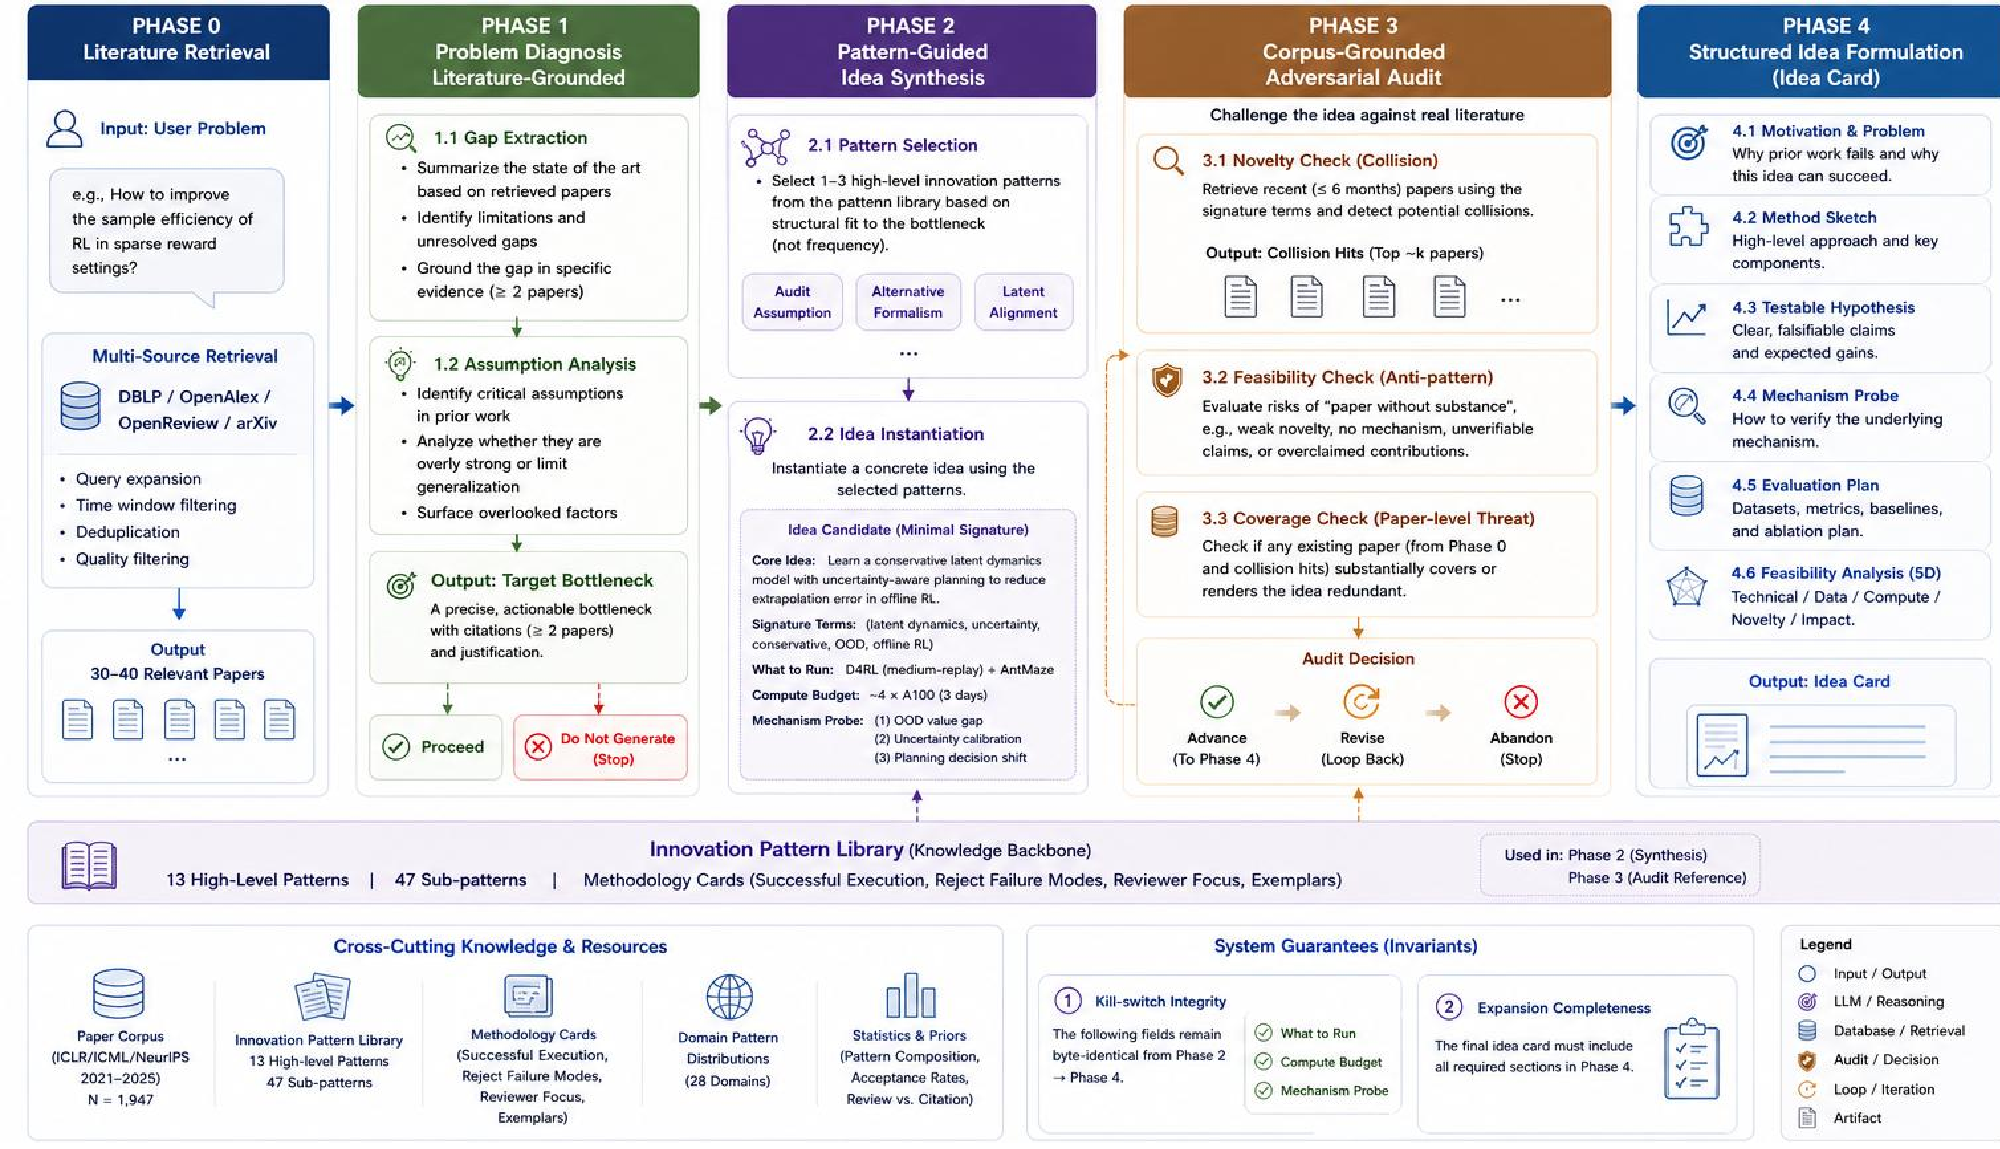
\includegraphics[width=\textwidth]{figures/fig_pipeline_generated.pdf}
\caption{Empirical substrate construction. The pipeline builds a 1{,}947-paper Oral / High-Cited / Reject corpus, extracts structured innovation signatures, embeds and clusters them to induce 13 high-level patterns and 47 sub-patterns, analyzes pattern composition and outcome variation, and converts the resulting taxonomy into operational methodology cards. The bottom band summarizes the substrate used downstream by NoveltySkill: a composable pattern space, domain-conditioned priors, review-vs-citation diagnostics, and audit-ready cards.}
\label{fig:pipeline}
\end{figure}

\textbf{(1) Discover, don't impose.} The innovation pattern taxonomy is induced by Claude Opus from the 47 empirically clustered tactics, with no seed categories supplied. Every Level-1 innovation pattern that appears in Section~\ref{sec:methodology} has a definition, an operational signature (verb--object template), and a set of clusters it subsumes; it was invented in response to the data, not before seeing it.

\textbf{(2) Contrast across the full acceptance spectrum.} We cluster Oral, High-Cited, and Rejected papers in the same embedding space, then compute per-pattern acceptance profiles. This exposes innovation patterns that the program committee rewards but the community does not adopt (e.g.\ \emph{Sharpen a Single Analytic Step}: oral=60, hc=1), and innovation patterns the community cites heavily but the PC treats more cautiously (e.g.\ \emph{Audit Evaluation via Controlled Perturbation}: hc=29, the highest HC share per unit Oral of any innovation pattern).

\textbf{(3) Separate domain from strategy before embedding.} We produce a second-pass \emph{domain-agnostic} rewrite of each paper's four innovation fields (abstract\_strategy, abstract\_key\_step, abstract\_why\_non\_obvious, abstract\_trigger\_condition) using Claude Sonnet. Embeddings are computed on these rewrites, not on the original domain-laden text. This converts clustering from a topic-similarity operation into a \emph{strategy-similarity} operation, which is what we want for innovation pattern induction.

\textbf{(4) Validate the taxonomy against the rejected population.} We re-cluster the 722 Rejected papers alone and ask Opus to map the resulting 23 reject-only clusters onto the 13-innovation pattern taxonomy induced from accepted papers. All but one cluster (\(n{=}12\), an adversarial-security subtheme) map cleanly. Rejected papers do not occupy a separate strategy space; they share the strategies of Oral papers but fail on execution-level criteria. This is the empirical lever NoveltySkill exploits: the gap to Oral is in \emph{execution criteria} (success conditions / failure modes / reviewer expectations), so the skill encodes these criteria from per-paper meta-reviews and uses them to audit candidate ideas.

\textbf{(5) Compose, don't choose.} A separate Opus pass independently re-tags every paper with all 13 innovation patterns, no upper cap. The result: 57.3\% of accepted papers execute exactly three innovation patterns; \(k{=}3\) is the modal composition size for Oral, HC, and Reject. The standout 3-way \emph{audit + reframing + shared-latent alignment} appears in 18 papers (12 Oral, 6 HC, 0 Reject), the dataset's only \(n{\geq}10\) composition with zero Rejected instances. The skill therefore generates 1--3-innovation pattern compositions with explicit roles (primary novelty action, supporting mechanism, validation action, framing action) rather than ranking single innovation patterns.

\subsection{Key findings}

Our analysis yields findings that stand independent of the downstream SKILL system:

\begin{enumerate}[leftmargin=1.5em]
\item \textbf{Thirteen induced innovation patterns.} Opus induces exactly 13 Level-1 innovation patterns from the 47 fine-grained clusters --- the count emerged, we did not specify it. The cluster-level mapping reaches 1{,}264 of 1{,}276 clustered papers (97\% of clustered; 65\% of full corpus). The independent paper-level multi-label tagging (\S\ref{subsec:multilabel}), which does not depend on cluster geometry, reaches all 1{,}947 papers including the 671 HDBSCAN-unclustered papers. The unclustered papers carry the same innovation pattern compositions as clustered ones (mean $k$ = 2.75 vs.\ 2.69) and have a slightly higher Oral acceptance rate (54.8\% vs.\ 50.8\%); the unclustered label means ``embedding lies between modal clusters,'' not ``outside the strategy space.''
\item \textbf{Oral-favored and Reject-favored innovation patterns are distinguishable.} Using the bias measure $\Delta = p_\text{oral} - p_\text{reject}$: Oral-favored innovation patterns (${+}1.1$ to ${+}4.2$ percentage points) include \emph{Reframe via Alternative Formalism} ($\Delta{=}{+}4.2$), \emph{Audit Evaluation via Controlled Perturbation} (${+}1.5$), and \emph{Sharpen a Single Analytic Step} (${+}1.3$); Reject-over-represented innovation patterns include \emph{Audit and Relax Implicit Assumption} (${-}3.0$), \emph{Align Heterogeneous Sources in Shared Space} (${-}2.8$), and \emph{Decompose and Recombine} (${-}1.4$). High-risk innovation patterns have high expected value \emph{if executed well}: \emph{Assumption Audit} produces the second-largest Oral pool (122 papers) despite its negative acceptance bias.
\item \textbf{PC-valued vs community-valued innovation patterns diverge.} \emph{Diagnose Then Surgically Fix} has a dramatic HC$\gg$Oral skew (47 HC vs 28 Oral): papers that precisely localize and patch a pathology get cited heavily but are rarely Oral-selected. Conversely, \emph{Sharpen a Single Analytic Step} has 60 Oral and only 1 HC---a classic PC-bias pattern (reviewers reward tight proofs; the community does not cite them).
\item \textbf{Multi-strategy is the norm.} 72\% of clustered papers receive a secondary innovation pattern. The top empirical pair is \emph{assumption audit} + \emph{formal reframing} (137 papers), followed by \emph{auxiliary signal} + \emph{shared latent alignment} (128) and \emph{analytic refinement} + \emph{assumption audit} (120).
\item \textbf{Conference and year profiles differ measurably.} ICML over-indexes on \emph{Reframe via Alternative Formalism} (18.3\%) and \emph{Sharpen a Single Analytic Step} (6.6\%); ICLR over-indexes on \emph{Diagnose Then Surgically Fix} (6.2\%); NeurIPS is the most balanced. Temporally, \emph{Audit Evaluation via Controlled Perturbation} more than tripled from 2023 (2.3\%) to 2024 (7.0\%), and \emph{Encode Invariance as Hard Constraint} climbed steadily from 2.6\% (2021) to 6.9\% (2025).
\end{enumerate}

\subsection{Contributions}

\textbf{Empirical contributions.}
(i) A data-induced 13-innovation pattern taxonomy with operational signatures, covering 47 fine-grained innovation sub-patterns and 28 induced research domains. The taxonomy is induced by Opus 4.7 from the data, not specified up front; the count of 13 emerged.
(ii) Per-innovation pattern acceptance and impact profiles across the full Oral / HC / Reject spectrum, including innovation patterns that are PC-rewarded but under-cited (e.g., \emph{Sharpen a Single Analytic Step}: 60 Oral, 1 HC) and innovation patterns the community cites heavily but the PC treats more cautiously (e.g., \emph{Diagnose Then Surgically Fix}: 47 HC, 28 Oral).
(iii) The negative result that rejected papers occupy the same strategy space as accepted ones, sharpening the research question from ``what strategies work?'' to ``what execution criteria separate same-strategy Oral from same-strategy Reject?''.
(iv) Paper-level multi-label re-tagging shows \(k{=}3\) is the modal composition size for accepted papers; the 3-way \emph{audit + reframing + shared-latent alignment} composition has 100\% accepted-class share in our sample.
(v) An induced 28-domain taxonomy + a \(28{\times}13\) joint matrix shows the 8 largest innovation patterns are \emph{domain-agnostic} in coverage (\(\geq 18/28\) domains) but \emph{domain-conditional} in acceptance rate (cell rates vary by tens of pp).

\textbf{Artifact contributions.}
(vi) Per-innovation pattern and per-sub-pattern operational ``cards'' generated by Opus 4.7: 13 eight-panel innovation pattern cards (step-by-step / success conditions / failure modes / Oral-vs-Reject gap / Oral-vs-HC gap / reviewer expectations / cognitive barriers / examples) and 47 six-panel innovation sub-pattern cards (tactical pattern / sibling differentiation / when-to-pick / tactical failure mode / representative Oral / representative Reject), every claim anchored to specific paper IDs and AC meta-reviews.
(vii) NoveltySkill: a model-agnostic two-tier skill (\texttt{novelty-skill} parent, \texttt{novelty-lit-search} sub-skill) implementing a 5-phase workflow that returns a single Oral-level research idea. Phase 0 retrieves $\sim$30--40 papers across DBLP / OpenAlex / OpenReview / arXiv with role-based time windows. Phase 1 (one LLM call) writes a literature-grounded bottleneck statement citing $\geq 2$ retrieved papers and routes to \texttt{proceed} or \texttt{do\_not\_generate}. Phase 2 (two LLM calls) selects an innovation-pattern composition by structural fit and generates one candidate with mechanism-specific \texttt{signature\_terms[]} for downstream collision retrieval. Phase 3 runs collision retrieval over a 6-month focused window (one orchestrator call, no LLM call) and a corpus-anchored audit (one LLM call) that performs three checks: composition-scoped reject-pattern scan against the candidate's chosen sub-pattern card plus any secondary patterns' methodology cards (typically 200+ cataloged reject lessons across the 47 sub-pattern cards); anti-pattern substantive-mitigation verification (the three corpus-validated reject-favored compositions with empirical Oral rates 30/39/44\%); and paper-pointed threat search across the unified pool of Phase-0 broad retrieval and Phase-3.1 mechanism-specific retrieval. The audit emits a verdict in \{\texttt{advance}, \texttt{revise}, \texttt{abandon}\} with a two-layer logic: a corpus-anchored hard floor (LLM cannot override) for triggered Reject patterns, refuted novelty claims, or exact-mechanism collisions; LLM soft judgment within the safe zone for advance vs revise. When the verdict is \texttt{revise}, a separate Phase-3.3 LLM call mechanically applies the audit's named revision targets, with kill-switch fields preserved byte-identical. Phase 4 expands the candidate into a structured idea card and renders PDF + Markdown + LaTeX. Two mechanical validators run as final contracts: \texttt{kill\_switch\_integrity} enforces byte-identical preservation of the falsification-anchor fields from Phase 2 through Phase 4, and \texttt{expansion\_completeness} verifies all required idea-card sections are present. The skill follows Anthropic's official skill best practices~\cite{anthropic_skill_bp_2025}: progressive disclosure, lean SKILL.md, scripts for deterministic steps, schema-validated phase boundaries, explicit OOD refusal. The skill produces the IDEA + an honest feasibility judgment; experimental engineering (datasets, baselines, ablations, expected figures) is the user's design responsibility, and no calendar projection is emitted.

\textbf{Open release.} Dataset (1947 papers with all extracted fields and innovation pattern assignments), the 13 + 47 cards (JSON and rendered LaTeX), the \(28{\times}13\) domain matrix, and both skills are released under permissive licensing.

\subsection{Roadmap}

Section~\ref{sec:related} surveys the rapidly-evolving 2025--2026 ideation, novelty-assessment, and scientific-discovery literature. Sections~\ref{sec:data}--\ref{sec:methodology} describe the dataset, the two-stage extraction, and the innovation-pattern induction. Section~\ref{sec:analysis} measures per-pattern acceptance and impact bias. Section~\ref{sec:domains} characterizes the induced domains and the innovation pattern breadth. Section~\ref{sec:trends} reports temporal and conference-level structure. Section~\ref{sec:reject} validates the taxonomy against the rejected population. Section~\ref{sec:ablation} ablates the embedding choice and the abstraction-stage decision. Section~\ref{sec:discussion} discusses limitations and threats to validity. Section~\ref{sec:skill} describes the SKILL system. The 13 innovation pattern cards and 47 sub-pattern cards are bundled in Appendices~\ref{app:cards} and~\ref{app:clusters}; the card-generation procedure is in Appendix~\ref{app:cards-method}.


%======================================================================
\section{Related Work}
\label{sec:related}
%======================================================================

The 2024--2026 literature on LLM research-idea generation has expanded rapidly along seven orthogonal axes. We position NoveltySkill against each in turn.

\subsection{End-to-end ``AI scientist'' systems}
\label{subsec:related-scientist}

End-to-end systems automate the full research lifecycle. AI~Scientist~\cite{lu2024aiscientist} drafts, implements, evaluates, and writes up research ideas in a single loop; its output was often judged incremental. AI-Researcher~\cite{airesearcher2025} extends this to autonomous innovation with structured architectures and decoupled training pipelines. Agent Laboratory~\cite{agentlab2025} accepts a human-supplied research idea and produces a research report and code, supporting variable human-in-the-loop. Idea2Plan~\cite{idea2plan2025} bridges idea to research plan via ReAct-style scaffolding with arXiv tools. The Sakana AI Scientist v2~\cite{sakana_v2} adds evolutionary-search refinement. Auto Research~\cite{autoresearch2025} structures a multi-agent framework spanning literature review, ideation, innovation pattern, experimentation, paper writing, and rebuttal. \emph{NoveltySkill differs}: it is not end-to-end; it terminates at a single Oral-grade idea-card output (with explicit failure paths when the audit cannot clear), leaving experimentation and writing to the user. The argument for stopping at the idea: end-to-end systems are bottlenecked by the same idea-quality gap our analysis characterizes; fixing the idea stage is upstream.

\subsection{Multi-agent and search-based ideation}
\label{subsec:related-multiagent}

VirSci~\cite{virsci2024} and IRIS~\cite{iris2025} model scientific teamwork as multi-agent collaboration with role-separated agents (ideator / reviewer / retriever). Deep Ideation~\cite{deepideation2025} introduces an explore-expand-evolve workflow over a scientific concept network, with a critic engine trained on real reviewer feedback (10.25\% improvement over baselines across four AI domains). Nova~\cite{nova2024} adds an iterative planning-and-search loop that purposely retrieves external knowledge to enrich each candidate, targeting the novelty-and-diversity gap in LLM ideation. The multi-workflow benchmark~\cite{multiworkflow2026} compares five reasoning architectures (reflection-based iterative refinement, Sakana evolutionary, Google Co-Scientist multi-agent, GPT Deep Research recursive decomposition, Gemini multimodal long-context) and finds decomposition-based and long-context workflows achieve mean novelty of 4.17/5. Alien Science~\cite{alienscience2026} formalizes a complementary creativity gap --- \emph{cognitive availability} (the likelihood a direction would be naturally proposed by a typical researcher) --- and learns to sample coherent but cognitively unavailable directions from clustered ``idea atoms.'' \emph{NoveltySkill differs}: rather than searching over candidate ideas, we constrain the LLM with empirically-derived innovation pattern cards encoding success conditions and failure modes from the Oral / HC / Reject contrast. Search and constraint are complementary: NoveltySkill could be embedded as the audit / constraint layer in any of the systems above.

\subsection{Methodology / pattern induction from accepted papers}
\label{subsec:related-induction}

The closest line of work to ours is innovation pattern induction from top-conference papers. Wang et al.~\cite{wang2024scireasoning} annotate Oral papers against a predefined 12-category taxonomy. MoRI~\cite{moRI2026} extracts \emph{motivation}\(\to\)\emph{innovation pattern} pairs from ICLR 2024--2025 accepted papers and trains a reasoning policy via supervised fine-tuning + controllable RL on dimensions of feasibility, novelty, and effectiveness. MotivGraph-SoIQ~\cite{motivgraph2025} builds a motivational knowledge graph and pairs it with Socratic dialogue for ideation. Navigating Ideation Space~\cite{navigating_ideation2026} decomposes scientific ideas into conceptual representations for positioning new ideas.

A parallel paradigm grounds idea generation in \emph{knowledge graphs} mined from large literature corpora. SciMuse~\cite{scimuse2024} builds a KG from 58 million research papers and conducts a 100-research-group-leader evaluation showing AI-generated ideas can be perceived as novel and impactful when grounded in cross-disciplinary KG paths. KG-grounded hypothesis generation~\cite{kghyp2024} similarly retrieves relevant KG sub-structures to constrain LLM hypothesis output and reports improved novelty + plausibility on biomedical benchmarks.

\emph{NoveltySkill differs from each}: (i) Wang's taxonomy is preset; ours is induced from data. (ii) MoRI fits a parametric policy; we deliver a structured non-parametric skill. (iii) The KG-based paradigms (SciMuse, KG-Hyp) ground ideas in concept-level co-occurrence; our taxonomy grounds ideas in \emph{strategic operations} (audit + relax assumption / sharpen analytic step / reframe via equivalence) extracted from how Oral and Reject papers differ in execution, not from concept adjacency. (iv) Critically, all six lines analyze \emph{only accepted} papers --- they do not contrast against rejection. Our 722-Reject pool yields the success-condition / failure-mode contrast that drives the skill's audit step, and the 100\%-Oral 3-way composition (\emph{audit + reframing + shared-latent alignment}) is invisible without the rejection contrast.

\subsection{Novelty assessment and prior-art collision}
\label{subsec:related-novelty}

A parallel thread builds tools that score whether a candidate idea collides with prior art. NovBench~\cite{novbench2026} is the first large-scale benchmark for novelty evaluation (1684 paper-review pairs, 4-dim eval framework: relevance / correctness / coverage / clarity). OpenNovelty~\cite{opennovelty2026} is an agentic system deployed on 500+ ICLR 2026 submissions producing transparent evidence-based novelty reports. GraphMind~\cite{graphmind2025} provides interactive novelty assessment tying paper key-elements to retrieved literature. Idea Novelty Checker~\cite{idea_novelty_checker2025} uses RAG with two-stage retrieve-then-rerank. Literature-Grounded Novelty Assessment~\cite{litgrounded2025} uses expert-annotated in-context examples to guide literature-grounded rationales. Augmenting Research Ideation with Data~\cite{augment_ideation2026} integrates metadata and automated preliminary-validation into ideation (+20\% feasibility, +7\% quality on social-science tasks). \emph{NoveltySkill incorporates this thread}: our \texttt{novelty-lit-search} sub-skill performs Phase-0 broad mapping and Phase-5 focused-window collision checking with a 7-class collision taxonomy; the action mapping is conditioned on the user-supplied novelty target (Oral / publication / Best Paper).

\subsection{Idea evaluation: feasibility, taste, and future impact}
\label{subsec:related-evaluation}

Si et al.~\cite{si2024llmideas} ran a 100+-NLP-researcher blind study showing LLM-generated ideas are rated \emph{more novel} but \emph{less feasible} than expert ideas. The follow-up execution study~\cite{si2026execution} reports that AI ideas score significantly lower than human ideas \emph{after} execution --- the gap is in operational criteria, not surface novelty. AI Can Learn Scientific Taste~\cite{ai_taste2026} trains a taste model on accepted/rejected pairs. HindSight~\cite{hindsight2026} evaluates LLM-generated ideas via future-citation impact. Learning to Predict Future-Aligned Research Proposals~\cite{future_aligned2026} predicts whether a candidate proposal aligns with future research directions. \emph{NoveltySkill incorporates the operational-criteria framing} from~\cite{si2026execution} as a primary motivation: the skill's audit phase performs three corpus-anchored checks (composition reject scan, anti-pattern verification, paper-pointed threat search) that surface execution-level gaps honestly --- when the audit cannot clear its hard floor it abandons rather than emits a degraded artifact.

\subsection{Benchmarks for ideation and discovery}
\label{subsec:related-benchmarks}

A wave of benchmarks now measures different aspects of ideation. IdeaBench~\cite{ideabench2024} evaluates research idea generation against referenced-work baselines. AI Idea Bench 2025~\cite{airesearchideas2025} curates 3495 papers from ICLR top-2\% and CVPR highlights as ground truth. ResearchBench~\cite{researchbench2025} decomposes scientific discovery into inspiration retrieval, hypothesis composition, and hypothesis ranking. NewtonBench~\cite{newtonbench2025} evaluates scientific-law discovery on 324 physics tasks with counterfactual law shifts. \emph{NoveltySkill is not a benchmark} and is downstream of these: our 1947-paper dataset and the per-paper innovation pattern assignments could serve as a complementary benchmark for ``does an ideation system reproduce the empirical Oral-favored composition patterns?''.

\subsection{Surveys, structured reasoning, and clustering substrate}
\label{subsec:related-substrate}

Two recent surveys map the landscape: ``From Automation to Autonomy''~\cite{from_automation_2025} (3-level taxonomy: Tool / Analyst / Scientist) and ``Towards Scientific Intelligence''~\cite{sci_intel_survey2025} (architectures / benchmarks / ethics). On the methodological-foundations side: chain-of-thought prompting~\cite{wei2022cot}, ReAct~\cite{yao2023react}, retrieval-augmented generation~\cite{lewis2020rag}, and Toolformer~\cite{schick2023toolformer} each attach a general-purpose capability to the LLM; SPECTER~\cite{cohan2020specter} provides citation-trained scientific embeddings; BERTopic~\cite{grootendorst2022bertopic} combines contextual embeddings with UMAP and HDBSCAN. Anthropic's official skill best-practices~\cite{anthropic_skill_bp_2025} guide our skill design: progressive disclosure, lean SKILL.md, deterministic scripts for repetitive steps, schema-validated phase boundaries, explicit triggers and negative cases. \emph{NoveltySkill's pipeline} embeds domain-agnostic strategy rewrites (rather than titles or abstracts) with OpenAI \texttt{text-embedding-3-large}; \S\ref{sec:ablation} shows that for strategy-level clustering the general-purpose embedder outperforms SPECTER2 because the relevant similarity is paraphrase-level rather than citation-level.

\subsection{Summary of differentiation}

Across these seven axes, NoveltySkill's distinctive moves are: \emph{(a)} contrast Oral / HC / Reject in the same embedding space (no other system uses Reject as a primary signal); \emph{(b)} induce the innovation pattern taxonomy from data (Wang~\cite{wang2024scireasoning} and MoRI~\cite{moRI2026} use predefined or motivation-driven schemas); \emph{(c)} deliver per-pattern operational cards with quoted reviewer evidence (no other system produces audit-ready cards anchored in meta-reviews); \emph{(d)} support multi-pattern compositions with explicit roles, justified by paper-level multi-label data showing \(k{=}3\) is the empirical mode; \emph{(e)} ship as a model-agnostic two-tier skill following Anthropic's official best practices, deployable to Claude Code, OpenAI assistants, Gemini, or open-weights LLMs without modification.


%======================================================================
\section{Dataset Construction}
\label{sec:data}
%======================================================================

\subsection{Scope and labeling}

We collect papers from ICLR, ICML, and NeurIPS for 2021--2025 via the OpenReview API (v1 for ICLR 2021--2023, v2 for ICLR 2024+, ICML 2023+, NeurIPS 2023+). ICLR 2020 is excluded from this release due to differing review-data schemas. For each paper we retain the title, abstract, author list, OpenReview id, decision string, full review set (rating, confidence, soundness, contribution, summary, strengths, weaknesses, questions), meta-review, and Semantic Scholar citation count.

Each paper receives zero or more of three labels. A paper may carry multiple labels (49 papers are simultaneously Oral and High-Cited).

\textbf{\textcolor{cblue}{Oral}} (1{,}014 papers): papers whose venue decision is Oral or Spotlight, representing what the program committee values most.

\textbf{\textcolor{cgold}{High-Cited (HC)}} (260 papers): top-30 most-cited papers per venue-year via authoritative citation CSVs, representing community adoption. For 2025 the top-10 most-cited are used because citation counts are still accumulating.

\textbf{\textcolor{cred}{Reject}} (722 papers): papers with an explicit Reject decision and a non-trivial review set, representing concrete failure signal.

Table~\ref{tab:data} shows the venue-year breakdown. The per-venue counts reflect two independent factors. First, \textbf{venue openness}: ICLR is OpenReview-native and publishes accept and reject decisions with full review threads, so its Reject pool is deepest; ICML and NeurIPS expose decisions on OpenReview only from 2023 onward and ICML 2023--2024 in particular release very few rejected submissions, which is why those rows show 0--3 in the Reject column. Second, \textbf{review accessibility}: even when a decision is published, the meta-review and reviewer comments are sometimes withheld or formatted such that automatic parsing fails---this is why metadata coverage (Section~\ref{subsec:meta-coverage}) shows only 340/1947 papers carrying a meta-review despite all 1947 having decisions. ICML 2025 is additionally excluded from the HC pool due to data-quality issues with the 2025 ICML citation source. These asymmetries are non-issues for the clustering stage but are treated carefully in the quantitative analysis (Section~\ref{sec:analysis}).

\begin{table}[htbp]
\centering
\caption{Dataset composition. Each column counts a paper if it carries that label; the same paper can appear in multiple columns. The Total row sums to $1{,}014+260+722=1{,}996$; the unique-paper count is $1{,}947$ after removing the $49$ Oral$\cap$HC overlaps. Per-class disjoint-pool counts used in Section~\ref{sec:analysis} are $1{,}014$ Oral, $211$ HC, $722$ Reject. ICLR 2020 is excluded.}
\label{tab:data}
\small
\begin{tabular}{llrrrr}
\toprule
\textbf{Venue} & \textbf{Year} & \textbf{\textcolor{cblue}{Oral}} & \textbf{\textcolor{cgold}{HC}} & \textbf{Oral$\cap$HC} & \textbf{\textcolor{cred}{Reject}} \\
\midrule
ICLR    & 2021 &  52 & 30 & 5 &   0 \\
ICLR    & 2022 &  49 & 30 & 5 &   0 \\
ICLR    & 2023 &  85 & 30 & 6 & 143 \\
ICLR    & 2024 &  63 & 30 & 1 & 138 \\
ICLR    & 2025 & 186 & 10 & 4 & 128 \\
ICML    & 2023 & 147 & 30 & 9 &   3 \\
ICML    & 2024 & 135 & 30 & 9 &   0 \\
ICML    & 2025 &  99 & 10 & 3 &  65 \\
NeurIPS & 2023 &  69 & 30 & 4 &  94 \\
NeurIPS & 2024 &  60 & 30 & 3 & 101 \\
NeurIPS & 2025 &  69 &  0 & 0 &  50 \\
\midrule
\textbf{Total} &  & \textbf{1{,}014} & \textbf{260} & \textbf{49} & \textbf{722} \\
\bottomrule
\end{tabular}
\end{table}

\subsection{Metadata coverage}
\label{subsec:meta-coverage}

After merging, 1{,}947 unique papers remain. All 1{,}947 carry the eight base fields and four abstracted fields (Section~\ref{sec:extract}). Metadata coverage varies: 1{,}074 papers carry the full abstract, 716 carry parsed reviews, 682 carry an extracted introduction, and 340 carry a meta-review. The Reject subset is particularly review-rich because rejection signal lives in the reviews.

\subsection{Splits}

We produce a stratified 80/20 train/test split over (venue, year, primary label) with seed 42: 1{,}557 train, 390 test. For buckets with $<5$ papers the whole bucket goes to train. All pattern discovery, innovation pattern induction, and acceptance analysis reported in this paper use the full 1{,}947 papers; the split is reserved for downstream SKILL evaluation in future work.

\subsection{Convention for in-paper paper references}
\label{subsec:paper-id-convention}

Throughout this paper we reference papers in the corpus by an internal identifier of the form \texttt{<VENUE>\_<YEAR>\_<NNNN>} (e.g., \texttt{ICLR\_2022\_0094}, \texttt{NeurIPS\_2023\_0753}). Each identifier resolves uniquely to an OpenReview submission via the \texttt{openreview\_id} field in the released dataset (\texttt{data/dataset/all\_records\_full.json}); a paper can be looked up at \texttt{https://openreview.net/forum?id=<openreview\_id>} after consulting the dataset. Of the 1{,}947 corpus papers, approximately 1{,}088 are referenced at least once in this report --- typically as evidence under a methodology card's success-condition or failure-mode list (e.g., ``evidence: \texttt{ICLR\_2022\_0094}, \texttt{ICML\_2023\_0551}, \ldots''). We do not include these as bibliography entries: a complete bib of the cited corpus would obscure the second-order related-work citations that constitute Section~\ref{sec:related}. The released dataset is the authoritative bibliographic resolution layer for any \texttt{paper\_id} appearing in this report. Where a specific corpus paper is discussed substantively in body text (e.g., the diffusion-ELBO paper~\cite{kingma2023diffusion} = \texttt{NeurIPS\_2023\_0753} that anchors our SKILL freshrun case study in Section~\ref{sec:skill}; LP-FT~\cite{kumar2022lpft} = \texttt{ICLR\_2022\_0094}, the DP continual-observation paper~\cite{henzinger2023dpcontinual} = \texttt{ICML\_2023\_0551}, EigenGame~\cite{gemp2021eigengame} = \texttt{ICLR\_2021\_0018}, and SAM-as-Bayes~\cite{mollenhoff2023sambayes} = \texttt{ICLR\_2023\_0331}, all of which feature as canonical examples in the methodology cards), a proper bibliography entry is provided.


%======================================================================
\section{Two-Stage Innovation-Signature Extraction}
\label{sec:extract}
%======================================================================

To convert each paper into a form amenable to strategy-level clustering we extract a twelve-field \emph{innovation signature}: eight base fields capturing the paper's domain-specific innovation story, plus four domain-agnostic rewrites of the most strategy-bearing fields.

\subsection{Stage 1: Eight base fields}

We feed Claude Sonnet the paper's title, abstract, introduction (extracted from the PDF), all reviews, and the meta-review, and request a structured output with the following fields:

\begin{enumerate}[nosep, leftmargin=1.5em]
\item \texttt{innovation\_approach}: one sentence describing \emph{how} this paper innovates as a reasoning strategy.
\item \texttt{key\_step}: the single most critical reasoning step from diagnosis to solution.
\item \texttt{why\_non\_obvious}: the cognitive barrier that blocked others from this approach.
\item \texttt{trigger\_condition}: domain-agnostic situation where this strategy applies, phrased as ``When X, apply Y to achieve Z.''
\item \texttt{reviewer\_praise}: three specific points the reviewers praised.
\item \texttt{reviewer\_concern}: three specific reviewer concerns.
\item \texttt{acceptance\_signal}: one sentence explaining what made the paper Oral / cited / rejected.
\item \texttt{contribution\_type}: one of \{theoretical, methodological, empirical, benchmark, system\}.
\end{enumerate}

Extraction is run under a JSON schema that enforces non-empty lists of length 3 for the two review-derived fields. All 1{,}947 papers pass the Stage-1 extraction.

\subsection{Stage 2: Four domain-agnostic rewrites}

A well-known failure mode of direct embedding is that the model latches onto domain nouns (``Transformer'', ``diffusion'', ``image'', ``molecule'') and produces topic clusters rather than strategy clusters. We defuse this by running a second Claude Sonnet pass that rewrites the first four base fields into their strategy-only equivalents. The prompt instructs the model to replace domain nouns with generic placeholders, adopt imperative phrasing (``Audit \ldots'', ``Transfer \ldots'', ``Design \ldots''), preserve the mechanism, and drop application detail. The resulting four fields are:

\begin{enumerate}[nosep, leftmargin=1.5em]
\item \texttt{abstract\_strategy} $\leftarrow$ \texttt{innovation\_approach}
\item \texttt{abstract\_key\_step} $\leftarrow$ \texttt{key\_step}
\item \texttt{abstract\_why\_non\_obvious} $\leftarrow$ \texttt{why\_non\_obvious}
\item \texttt{abstract\_trigger\_condition} $\leftarrow$ \texttt{trigger\_condition}
\end{enumerate}

A representative contrast illustrates the shift: for the paper \emph{High Fidelity Speech Synthesis with Adversarial Networks}, \texttt{innovation\_approach} reads ``\textit{They solved a domain transfer problem by borrowing the PatchGAN multi-scale discriminator strategy from image GANs and re-instantiating it at multiple temporal windows in audio, adding conditioning signals to close the fidelity gap}'' whereas \texttt{abstract\_strategy} reads ``\textit{Transfer a multi-scale discrimination strategy from one data modality to another by re-instantiating it at the appropriate domain-specific granularity, then add conditioning signals to close the remaining fidelity gap.}'' The generic version is what we feed into the embedding model.

All four abstract fields are populated for 1{,}947/1{,}947 papers.


%======================================================================
\section{Unsupervised Pattern Discovery}
\label{sec:clustering}
%======================================================================

\subsection{Embedding}

We concatenate the four abstract fields per paper with explicit \texttt{field: content} prefixes (average length 1{,}185 characters) and embed with OpenAI \texttt{text-embedding-3-large} (3{,}072 dimensions). Vectors are L2-normalized.

\subsection{Clustering}

UMAP reduces the 3{,}072-dim cosine-normalized space to 10 dimensions ($n\_\text{neighbors}{=}15$, $\min\_\text{dist}{=}0$, seed 42), and HDBSCAN ($\min\_\text{samples}{=}\lceil \min\_\text{cluster\_size}/3 \rceil$, \texttt{cluster\_selection\_method}=\texttt{eom}) clusters the reduced space. We sweep $\min\_\text{cluster\_size}\in\{10,15,20,25,30,40\}$ and pick the configuration that maximizes silhouette subject to unclustered fraction $<0.20$; when no configuration meets the unclustered cap we report the highest-silhouette one. Table~\ref{tab:sweep} shows the ALL-set sweep.

\begin{table}[htbp]
\centering
\caption{HDBSCAN sweep on the full 1{,}947-paper embedding. Selected row bolded.}
\label{tab:sweep}
\small
\begin{tabular}{cccccc}
\toprule
$\min\_\text{cluster\_size}$ & $k$ & $n_\text{unclustered}$ & \% unclustered & silhouette \\
\midrule
\textbf{10} & \textbf{47} & \textbf{671} & \textbf{34.5} & \textbf{0.474} \\
15 & 30 & 679 & 34.9 & 0.425 \\
20 & 18 & 839 & 43.1 & 0.432 \\
25 & 19 & 845 & 43.4 & 0.497 \\
30 & 13 & 862 & 44.3 & 0.482 \\
40 &  9 & 869 & 44.6 & 0.433 \\
\bottomrule
\end{tabular}
\end{table}

We pick $\min\_\text{cluster\_size}{=}10$ despite its slightly lower silhouette than the $=25$ row because it identifies 47 innovation sub-patterns while keeping unclustered fraction stable at 34.5\%. Coarsening min\_cluster\_size does not reduce the unclustered fraction (it hovers near 34--44\% across the sweep), meaning the additional unclustered points'' at fine granularity is not recovered by coarsening --- those points are genuinely far from all density peaks.

\paragraph{What ``unclustered'' actually means (and why we don't call it ``noise'').} HDBSCAN's standard nomenclature labels points outside any density peak as ``noise''. We use ``unclustered'' throughout this paper because, as the analysis below shows, the property is geometric (between modal clusters) rather than substantive (idiosyncratic outliers / low-quality papers / strategies outside the innovation pattern framework). The 34.5\% of papers HDBSCAN flags are \emph{not} strategy-empty: unclustered and clustered papers have nearly identical paper-level multi-label innovation pattern compositions (mean $k = 2.75$ vs.\ $2.69$; $k{=}3$ is 56.8\% in unclustered vs.\ 57.6\% in clustered; 100\% of both groups have all four \texttt{abstract\_*} fields populated with comparable median lengths $\sim 220$--$280$ chars). Unclustered papers also have a slightly \emph{higher} Oral acceptance rate (54.8\% vs.\ 50.8\% for clustered). The unclustered label is a property of \emph{embedding geometry under the chosen mcs threshold}, not a property of strategic content: a paper whose strategy embedding lands at the boundary between two or three modal clusters --- typically because its three executed innovation patterns are weighted comparably in the rewritten text --- is flagged unclustered even though its innovation pattern composition is identical to clustered papers'. In short, ``unclustered'' here means \emph{between modal clusters}, not \emph{outside the strategy space}. The 13-innovation pattern framework, which operates at the paper level via independent multi-label tagging (\S\ref{subsec:multilabel}), covers unclustered and clustered papers equally.

\subsection{What the 47 clusters look like}

Cluster sizes (excluding unclustered) range from 10 (the smallest valid size) to 115, with mean 27.1 and median 18. The largest clusters are:

\begin{itemize}[nosep, leftmargin=1.5em]
\item \textbf{C24} (\(n{=}115\)): \emph{Unified Cross-Modal Latent Space Alignment}---projecting heterogeneous modalities or task formats into a single shared space.
\item \textbf{C35} (\(n{=}93\)): \emph{Benchmark Validity Auditing via Controlled Perturbation}.
\item \textbf{C15} (\(n{=}93\)): \emph{Tight Bound Recovery via Targeted Proof Refinement}.
\item \textbf{C31} (\(n{=}79\)): \emph{Bottleneck Audit with Targeted Component Substitution}.
\item \textbf{C22} (\(n{=}71\)): \emph{Generative Reframing of Sequential Decision Problems}.
\end{itemize}

Each cluster is automatically labeled by an additional Claude Sonnet pass that consumes the cluster's eight centroid-nearest representative papers and produces a 2--6 word label plus a one-sentence description. A second Opus 4.7 pass then produces a level-2 \emph{disambiguation card} for each cluster (\S\ref{subsec:multistrat} uses the resulting tactic-level patterns; full cards in App.~\ref{app:clusters}). Each disambiguation card has six panels: (1) \emph{tactical\_pattern} --- the cluster's specific reasoning move at the granularity below the level-1 innovation pattern; (2) \emph{differentiation\_within\_parent} --- what distinguishes this cluster from its sibling clusters that share the same level-1 parent; (3) \emph{when\_to\_pick\_this\_one} --- the situational trigger conditions under which this sub-pattern is the right choice; (4) \emph{tactical\_failure\_mode} --- the cluster-specific failure shape that recurs in its Reject papers; (5) \emph{representative\_oral} --- one Oral exemplar with a one-line lesson; (6) \emph{representative\_reject} --- one Reject exemplar with a one-line lesson. We use the 47-cluster inventory as raw material for innovation pattern induction in the next section.

\subsection{Per-cluster acceptance composition: which clusters are safe vs.\ warning}
\label{subsec:clusterskew}

Although the embedding (Fig.~\ref{fig:umap}b) interleaves Oral, HC, and Reject papers across most clusters, the cluster-level proportions are highly non-uniform. Figure~\ref{fig:cluster_skew} shows each of the 47 clusters' Oral / HC / Reject composition, sorted by Oral rate. Two flagging rules let us partition the clusters into actionable categories for downstream use (the SKILL retrieval layer pre-filters on these flags):

\begin{itemize}[leftmargin=1.4em, topsep=2pt, itemsep=2pt]
\item \textbf{Oral-safe} ($p_O \geq 65\%$ and $n_O \geq 5$): \textbf{12 clusters}. These are the clusters whose tactic, when properly executed, lands at the top of the acceptance distribution. The five sharpest are C07 \emph{Timescale Separation for Staged Dynamics Analysis} (11/0/0, 100\% Oral), C08 \emph{Formal Abstraction for Tight Expressivity Bounds} (14/1/1, 88\%), C01 \emph{Symmetry Exploitation via Equivariant Architecture} (17/2/1, 85\%), C45 \emph{Generative Framework Generalization via Mathematical Reformulation} (17/0/3, 85\%), and C09 \emph{Structural Inductive Bias Formalization} (16/1/2, 84\%).
\item \textbf{Reject-warn} ($p_R \geq 65\%$ and $n_R \geq 5$): \textbf{5 clusters}. These tactics are present in accepted work but rarely succeed; the SKILL should warn rather than recommend. They are C42 \emph{Decompose-then-Recombine Multi-Objective Search} (1/0/10, 91\% Reject), C04 \emph{Soft Uncertainty Preservation via Probabilistic Reformulation} (3/0/12, 80\%), C13 \emph{Global Structure Recovery via Local Proxy Decomposition} (3/0/11, 79\%), C19 \emph{Relational Structure Critique and Realignment} (2/2/14, 78\%), and C20 \emph{Supervision Redesign via Training Signal Audit} (1/2/7, 70\%).
\item \textbf{Mixed}: the remaining 30 clusters. These tactics produce both Oral and Reject papers in comparable shares; they are the bulk of the working space, and acceptance hinges on the per-paper success conditions and failure modes characterized in the methodology cards (\S\ref{subsec:cards}, App.~\ref{app:cards}).
\end{itemize}

The per-cluster labels and full counts are in \texttt{clustering/extra/cluster\_composition.csv}.

\paragraph{These flags are risk signals, not recommendation labels.} \emph{Oral-safe} does not mean ``preferred''; \emph{Reject-warn} does not mean ``forbidden''. They are statistical priors with limited sample sizes, sensitive to year, conference, and topic saturation, and a Reject-warn cluster's reject papers may have failed on execution rather than tactic choice. We therefore expose these flags as informational signals available to downstream consumers but do not gate recommendation on them; a user whose problem genuinely matches a Reject-warn cluster's tactic is free to proceed and is informed of the cluster's documented failure modes via the sub-pattern card.

\begin{figure}[H]
\centering
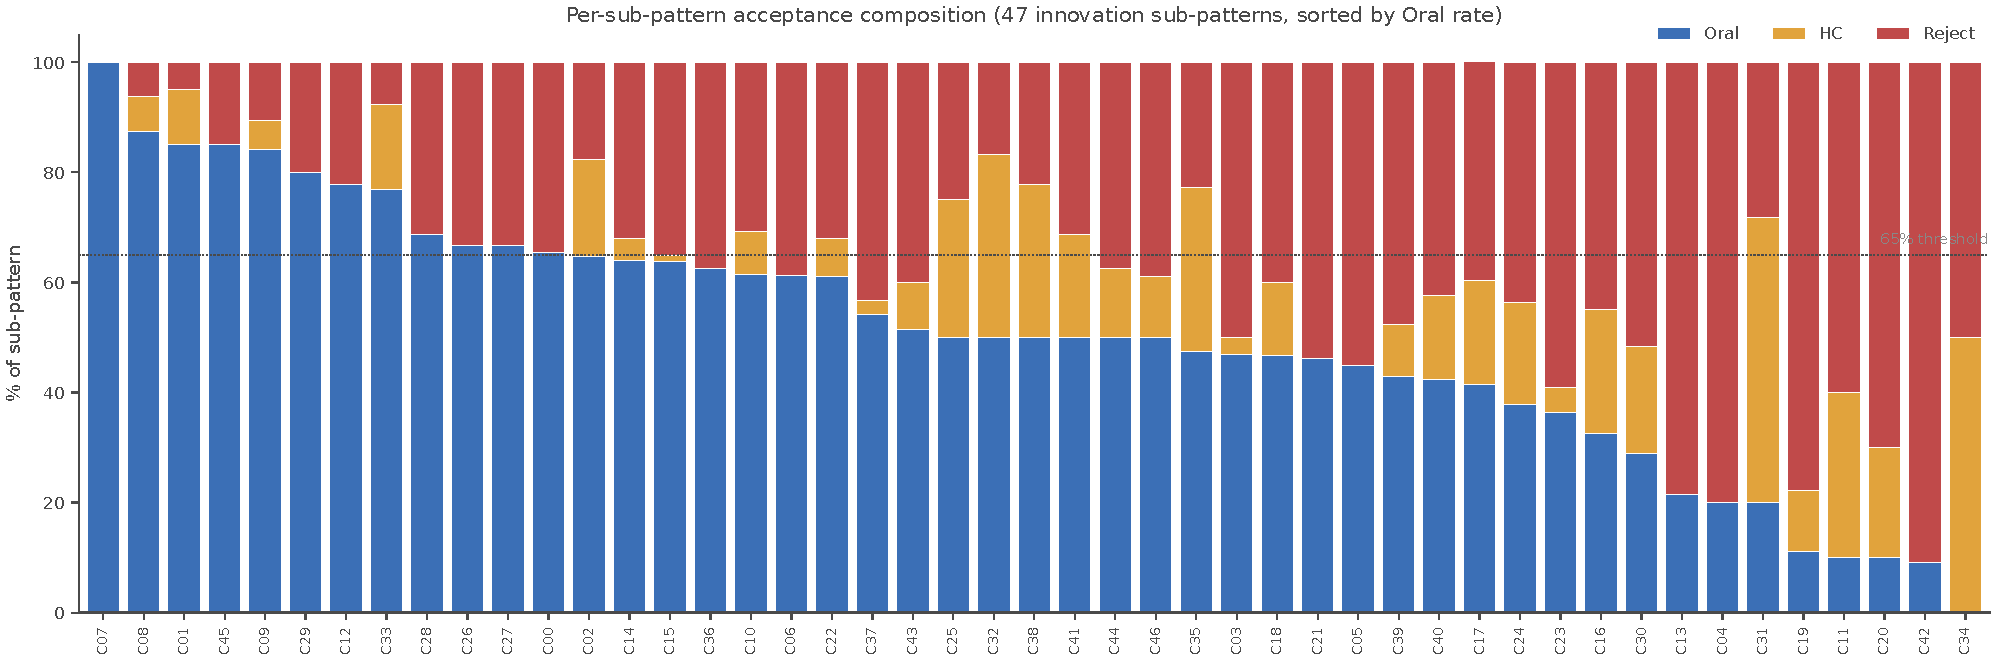
\includegraphics[width=0.96\textwidth]{figures/fig_cluster_skew.pdf}
\caption{Acceptance composition of the 47 clusters, sorted by Oral rate. Twelve clusters cross the 65\% Oral threshold (left); five cross the 65\% Reject threshold (right). The remaining 30 are mixed.}
\label{fig:cluster_skew}
\end{figure}

\begin{figure}[H]
\centering
\begin{subfigure}[b]{0.50\textwidth}
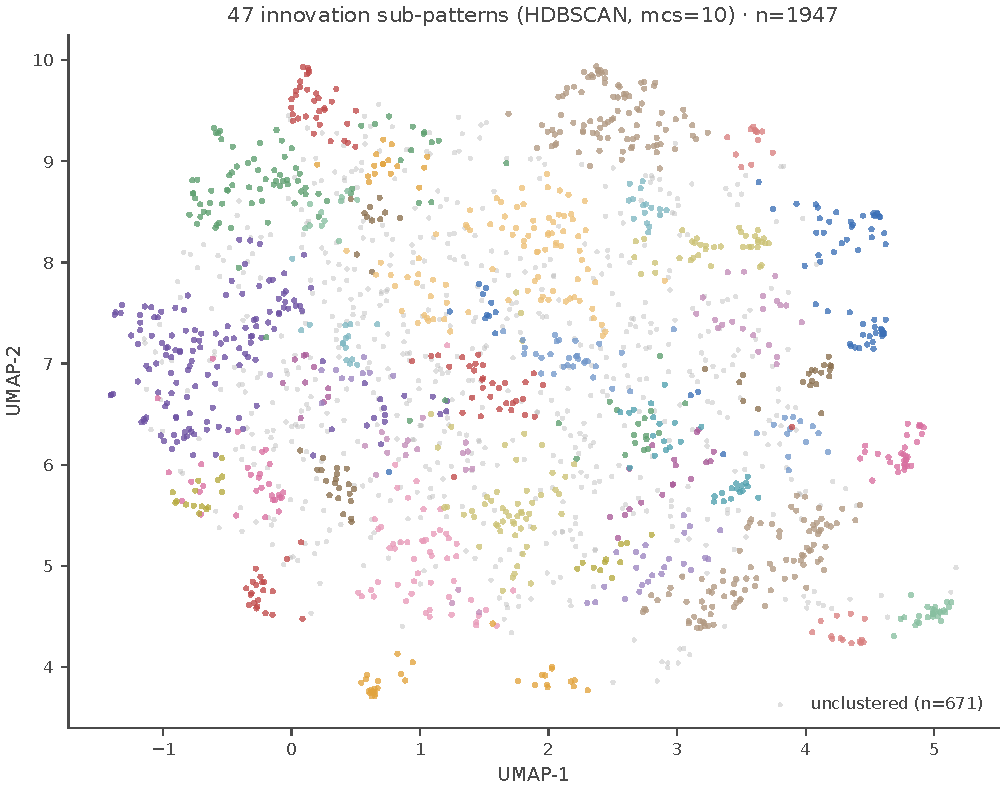
\includegraphics[width=\textwidth]{figures/fig_umap_clusters.pdf}
\caption{47 clusters, colored; unclustered in gray.}
\end{subfigure}
\hfill
\begin{subfigure}[b]{0.42\textwidth}
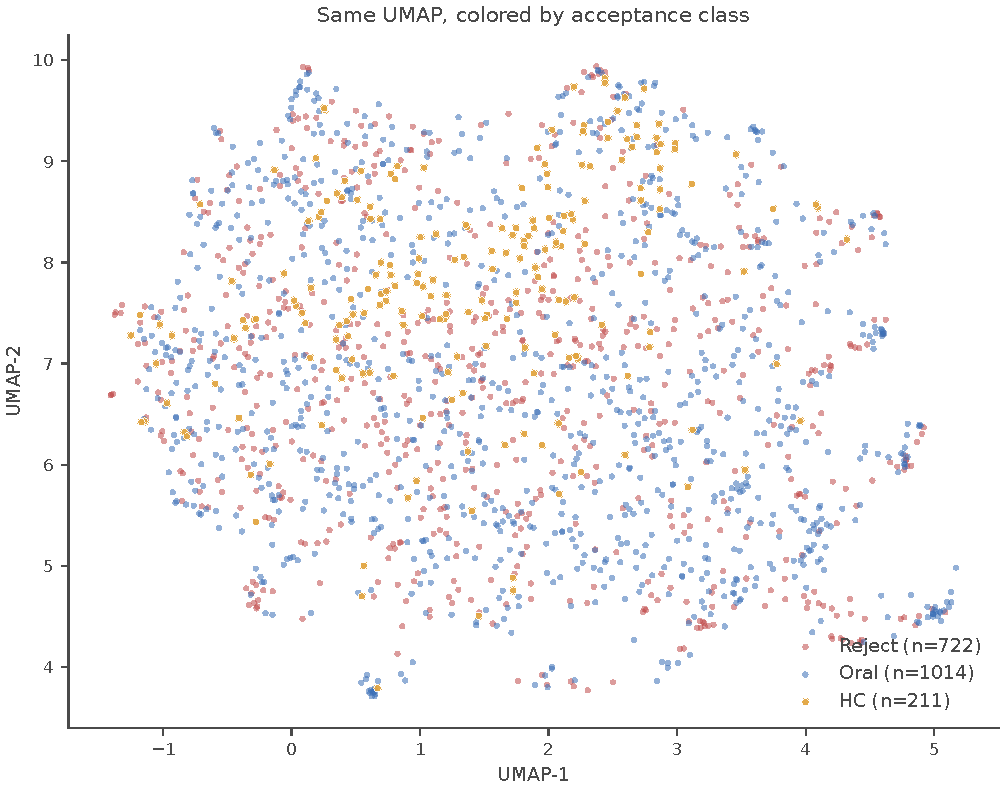
\includegraphics[width=\textwidth]{figures/fig_umap_label.pdf}
\caption{Colored by label (Oral / HC / Reject).}
\end{subfigure}
\caption{2D UMAP projection of the 1{,}947-paper embedding. Oral, HC, and Reject papers are interleaved across essentially every cluster: the embedding captures strategy, not acceptance.}
\label{fig:umap}
\end{figure}


%======================================================================
\section{Methodology Induction}
\label{sec:methodology}
%======================================================================

Fine-grained innovation sub-patterns answer ``what specific move did this paper make?'' but not ``what kind of move is that?''. For the latter we ask Claude Opus 4.7 to induce a Level-1 innovation pattern taxonomy from the 47 clusters, with the only prompt-level constraints being (a) produce between 6 and 18 entries, (b) every entry must describe a reusable reasoning strategy (not a domain, not a venue), (c) every entry must include a definition, an operational signature, and a when-to-apply clause, and (d) every one of the 47 clusters must be mapped to a primary innovation pattern plus an optional secondary.

Opus returns a 13-innovation pattern taxonomy (Table~\ref{tab:tax}) and a 47-cluster mapping in a single structured call. We make no edits to either. The 13 innovation patterns are:

\begin{table}[htbp]
\centering
\caption{The 13 induced innovation patterns. \(n_\text{cl}\)=fine-grained clusters mapped as primary; Oral / HC / Reject counts are paper-level primary-mapping counts.}
\label{tab:tax}
\small
\begin{tabular}{p{7cm} c rrrr}
\toprule
\textbf{Methodology (id)} & \textbf{\(n_\text{cl}\)} & \textbf{Oral} & \textbf{HC} & \textbf{Reject} & \textbf{Total} \\
\midrule
Reframe via Alternative Formalism \texttt{(formal\_reframing)}      & 9 & 162 & 21 & 85 & 268 \\
Audit and Relax Implicit Assumption \texttt{(assumption\_audit)}    & 11 & 122 & 23 & 108 & 253 \\
Align Heterogeneous Sources in Shared Space \texttt{(shared\_latent)} & 1 & 45 & 22 & 52 & 119 \\
Encode Invariance as Hard Constraint \texttt{(invariance\_constraint)} & 6 & 62 & 5 & 36 & 103 \\
Diagnose Then Surgically Fix \texttt{(surgical\_fix)}               & 2 & 28 & 47 & 27 & 102 \\
Audit Evaluation via Controlled Perturbation \texttt{(eval\_audit)} & 1 & 46 & 29 & 22 & 97 \\
Sharpen a Single Analytic Step \texttt{(analytic\_refinement)}      & 1 & 60 & 1 & 33 & 94 \\
Exploit Redundancy via Compression \texttt{(redundancy\_compression)} & 2 & 31 & 13 & 29 & 73 \\
Decompose and Recombine \texttt{(decomposition)}                    & 5 & 31 & 5 & 32 & 68 \\
Engineer Auxiliary Supervision Signal \texttt{(auxiliary\_signal)}  & 5 & 23 & 9 & 24 & 56 \\
Localize via Causal Probing \texttt{(mechanistic\_probing)}         & 2 & 29 & 6 & 20 & 55 \\
Soft Probabilistic Relaxation \texttt{(soft\_relaxation)}           & 1 & 3 & 0 & 12 & 15 \\
Aggregate Over Diverse Candidates \texttt{(candidate\_aggregation)} & 1 & 6 & 3 & 3 & 12 \\
\midrule
\textit{Noise (no primary)} &  & 368 & 76 & 239 & 683 \\
\bottomrule
\end{tabular}
\end{table}

Each innovation pattern is specified to the level of operational detail needed to be actionable; full definitions, operational signatures (the \texttt{step\_by\_step} panel), and when-to-apply clauses are provided verbatim in the per-pattern cards in Appendix~\ref{app:cards}.

\paragraph{Non-mutually-exclusive operators.} The 13 innovation patterns are \emph{not} mutually exclusive innovation classes. Several pairs naturally overlap --- e.g., \emph{Audit and Relax Implicit Assumption} vs.\ \emph{Reframe via Alternative Formalism} (a reframing often exposes a hidden assumption); \emph{Diagnose Then Surgically Fix} vs.\ \emph{Localize via Causal Probing} (causal probing is a diagnostic instrument); \emph{Engineer Auxiliary Supervision Signal} vs.\ \emph{Align Heterogeneous Sources in Shared Space} (multi-modal distillation typically does both). The cluster-level mapping forces a single primary per cluster for organizational reasons, but the underlying papers genuinely execute multiple operators in composition. The paper-level multi-label tagging in \S\ref{subsec:multilabel} confirms this empirically (\(k{=}3\) is the modal composition size). \emph{The right way to read the 13 innovation patterns is as innovation operators, where a paper is represented as a composition of operators rather than assigned to a single category.}

\paragraph{A note on small-sample innovation patterns.} Two innovation patterns have small per-paper-primary populations: \emph{Soft Probabilistic Relaxation} ($n{=}15$ papers) and \emph{Aggregate Over Diverse Candidates} ($n{=}11$). These are valid \emph{operators} --- the underlying clusters are statistically distinct in embedding space --- but they are \textbf{low-support operators}: their per-pattern acceptance statistics rest on thin evidence and should not be used as strong recommendation priors. The corresponding cards (App.~\ref{app:cards}) are auto-flagged as \texttt{confidence: low}, and downstream consumers (including the SKILL's Phase 2.1 selection step) read this flag and surface the low-support warning rather than gating these innovation patterns out of recommendation. They remain available for ideation when the user's problem genuinely fits.

\paragraph{Plain-language aliases.} The innovation pattern names use compact technical phrasing for analytical precision (\emph{Audit and Relax Implicit Assumption}, \emph{Encode Invariance as Hard Constraint}, etc.). Each innovation pattern also carries a \emph{plain-language alias} that the SKILL surfaces in user-facing output to keep the framework legible to non-specialists: e.g., \emph{Audit and Relax Implicit Assumption} $\to$ ``Find the hidden assumption and weaken it''; \emph{Reframe via Alternative Formalism} $\to$ ``Change the mathematical lens''; \emph{Diagnose Then Surgically Fix} $\to$ ``Find the failure point and patch only that''. The full alias map is in the per-pattern cards (\texttt{plain\_alias} field) of Appendix~\ref{app:cards}.

\subsection{From definition to operational card}
\label{subsec:cards}

A definition + operational signature tells a researcher \emph{what} the innovation pattern is, but not \emph{when it lands and when it doesn't}. To answer the latter we run a second Opus 4.7 pass per innovation pattern, feeding all of its Oral, HC, and Reject papers (with their abstract$_*$ fields and AC meta-reviews; 83\% review coverage after a separate review-recovery pass; see Appendix~\ref{app:cards-method}) and asking for a structured card with eight panels: (1) \emph{step\_by\_step} --- a 6-step procedural recipe for executing the pattern; (2) \emph{success\_conditions} --- cross-Oral patterns of what makes the pattern land; (3) \emph{failure\_modes} --- cross-Reject patterns of how it fails; (4) \emph{oral\_reject\_gap} --- the prose contrast between the two pools; (5) \emph{oral\_hc\_gap} --- the prose contrast between PC-favored and community-favored execution; (6) \emph{reviewer\_expectations} --- bullets tagged by provenance (\texttt{[oral\_reviews]}, \texttt{[reject\_reviews]}, \texttt{[both]}); (7) \emph{cognitive\_barriers} --- the field-level blind spots that make the pattern non-obvious; (8) \emph{representative\_examples} --- 6--8 paper-anchored exemplars (Oral and Reject), each with a one-line lesson. Every claim must cite $\geq 2$ \texttt{paper\_id}s; the model is instructed to set \texttt{confidence=low} when sample sizes or meta coverage fall below thresholds and to refuse the Oral-vs-HC contrast when $n_{HC}<5$.

The 13 resulting cards comprise the operational substrate of the SKILL system: each card's success conditions become positive constraints on idea generation, its failure modes become guardrails, its Oral-vs-Reject gap becomes the discrimination signal during ranking, and its representative examples become the few-shot exemplars. The seven cards with \texttt{confidence=high} carry the load; three medium and three low cards are still emitted but flagged. The full 13 cards are in Appendix~\ref{app:cards}; readers are pointed in particular at the cards for \emph{Audit and Relax Implicit Assumption} and \emph{Reframe via Alternative Formalism}, which are the secondary and primary innovation patterns of the freshrun end-to-end candidate (\S\ref{subsec:skill-workflow}) and form a continuous trail from corpus card to running case study.

\subsection{Coverage and granularity}

The 13 innovation patterns have two coverage figures, and we report both because they answer different questions:
\begin{itemize}[leftmargin=1.4em, topsep=2pt, itemsep=2pt]
\item \textbf{Cluster-level coverage}: 1{,}264 of 1{,}276 clustered papers (97\% of clustered; 65\% of the full 1{,}947-paper corpus) receive a primary innovation pattern by inheritance from their innovation sub-pattern. The 12 papers without primary fall in the single out-of-taxonomy reject cluster (\S\ref{sec:reject}).
\item \textbf{Paper-level multi-label coverage}: \emph{all} 1{,}947 papers, including the 671 HDBSCAN-unclustered papers, receive a non-empty innovation pattern assignment from the independent multi-label tagging pass (\S\ref{subsec:multilabel}). The 13-innovation pattern framework therefore covers the corpus completely at the paper level, even though only 65\% of papers are assignable via the cluster-level inheritance.
\end{itemize}
The distribution has a long tail. By cluster-level primary count, the top three innovation patterns (\emph{formal reframing}, \emph{assumption audit}, \emph{shared latent alignment}) account for 640 papers; the bottom three (\emph{soft relaxation}, \emph{candidate aggregation}, and \emph{mechanistic probing}) account for 82. This matches the cluster-level pattern: many innovations use a small number of deeply-worked strategies; a long tail uses rare ones.

The joint hierarchy exposes both each innovation pattern's paper volume / Oral--HC--Reject mix and how many fine-grained tactical clusters each parent pattern decomposes into. Two empirical observations are immediate:

\textbf{(i) Methodology fragmentation is uneven.} \emph{Audit and Relax Implicit Assumption} (250 papers) decomposes into 11 distinct innovation sub-patterns; \emph{Reframe via Alternative Formalism} (259) into 9; \emph{Encode Invariance as Hard Constraint} (101) into 6. By contrast, \emph{Align Heterogeneous Sources in Shared Space} (115), \emph{Audit Evaluation via Controlled Perturbation} (93), and \emph{Sharpen a Single Analytic Step} (93) are each a single large cluster --- the innovation pattern operates at one consistent tactical granularity. The 11-cluster decomposition under \emph{Audit and Relax} is not over-fragmentation: the underlying clusters distinguish substantively different audit-relax moves (e.g., audit a generative-model identifiability assumption vs.\ audit an evaluation-protocol assumption vs.\ audit a privacy-budget assumption).

\textbf{(ii) Cluster sizes follow a long-tail distribution.} Cluster sizes range from 10 to 115 (mean 27.1, median 18). Of 47 clusters, 13 are small ($n<15$); the corresponding tactical cards (App.~\ref{app:clusters}) are auto-flagged as \texttt{confidence: low}. We do not merge these small clusters into their parents because (a) HDBSCAN at $\textit{mcs}{=}10$ has already enforced the minimum size, (b) the cards' confidence flags transparently expose the thin-evidence status to downstream users, and (c) some small clusters carry strong consistent signals (e.g., C04 \emph{Soft Probabilistic Relaxation} with 11/15 reject papers is the dataset's clearest reject-warn cluster --- merging it into a larger parent would dilute that signal).

\begin{figure}[htbp]
\centering
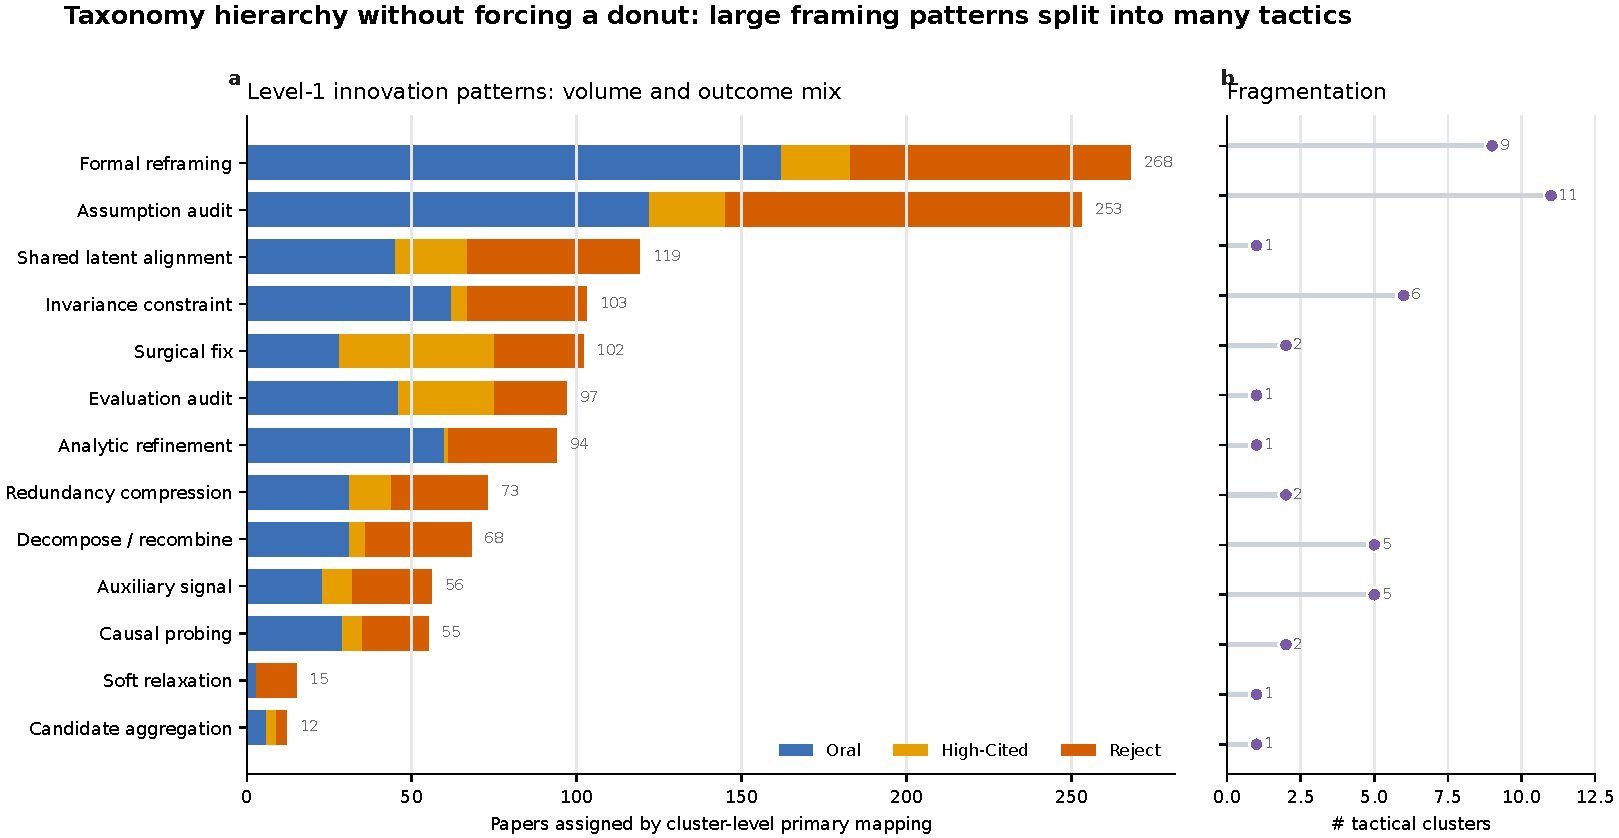
\includegraphics[width=\textwidth]{figures/fig_hierarchy_donut.pdf}
\caption{Hierarchical paper distribution. Panel (a): the 13 induced Level-1 innovation patterns, sorted by cluster-level primary paper count and stacked by outcome class. Panel (b): the number of fine-grained tactical clusters under each parent innovation pattern. Framing patterns such as audit and reframing have both high volume and high fragmentation; execution and validation patterns such as shared-latent alignment, evaluation audit, and analytic refinement are more tactically concentrated.}
\label{fig:hierarchy_donut}
\end{figure}

\subsection{Multi-strategy assignments}
\label{subsec:multistrat}

This subsection presents the cluster-level view of multi-strategy composition. The cluster-level mapping caps at \emph{primary~+~secondary} per paper by construction; the deeper paper-level multi-label view that recovers the true \(k{=}3\) modal composition, including the 671 HDBSCAN-unclustered papers excluded here, is reported in \S\ref{subsec:multilabel} and should be read as the authoritative composition analysis.

\textbf{Paper-level coverage of the secondary slot.} Cluster-level (primary, secondary) propagates to per-paper. Of the 1{,}947 papers, 671 (34.5\%) fall into the HDBSCAN-unclustered bucket and have no cluster-level primary innovation pattern (though they have full paper-level multi-label assignments, see \S\ref{subsec:multilabel}); of the remaining 1{,}276 clustered papers, 923 (72.3\%) carry both a primary and a non-trivial secondary, and 353 (27.7\%) carry only a primary (their cluster's secondary slot was empty in the Opus mapping). Multi-strategy assignment is therefore the norm among coherently-clustered papers.

Table~\ref{tab:combos} lists the top primary$+$secondary combinations and their acceptance breakdown. Combinations are unordered pairs; the count is the number of papers whose cluster's primary$/$secondary maps to exactly this pair.

\begin{table}[htbp]
\centering
\caption{Methodology combinations with $n{\geq}20$, sorted by Oral-vs-Reject rate $p_O = n_O / (n_O + n_R)$. Baseline $p_O$ across the dataset is $\mathbf{58.4\%}$ (1014 Oral, 722 Reject). $\Delta p_O$ is the combination's deviation from the baseline. Combinations $>+5\,$pp\ are Oral-favored; combinations $<-5\,$pp\ are Reject-favored.}
\label{tab:combos}
\small
\begin{tabular}{p{8.6cm} rrr r r}
\toprule
\textbf{Combination} & \textbf{Oral} & \textbf{HC} & \textbf{Reject} & \textbf{$p_O$} & \textbf{$\Delta p_O$} \\
\midrule
\textit{analytic refinement} + \textit{assumption audit}            &  81 &  0 &  39 & 67.5\% & $+9.0$ \\
\textit{assumption audit} + \textit{formal reframing}               &  88 &  5 &  44 & 66.7\% & $+8.2$ \\
\textit{invariance constraint} + \textit{shared latent alignment}   &  18 &  0 &   9 & 66.7\% & $+8.2$ \\
\textit{decomposition} + \textit{formal reframing}                  &  28 &  3 &  15 & 65.1\% & $+6.7$ \\
\midrule
\textit{mechanistic probing} + \textit{surgical fix}                &  20 &  1 &  16 & 55.6\% & $-2.9$ \\
\textit{assumption audit} + \textit{mechanistic probing}            &  14 &  4 &  14 & 50.0\% & $-8.5$ \\
\textit{formal reframing} + \textit{invariance constraint}          &  18 &  0 &  19 & 48.6\% & $-9.8$ \\
\textit{auxiliary signal} + \textit{shared latent alignment}        &  51 & 18 &  59 & 46.4\% & $-12.1$ \\
\textit{assumption audit} + \textit{surgical fix}                   &  32 & 39 &  40 & 44.4\% & $-14.0$ \\
\textit{formal reframing} + \textit{redundancy compression}         &  13 &  5 &  18 & 41.9\% & $-16.5$ \\
\textit{assumption audit} + \textit{invariance constraint}          &  20 &  6 &  31 & 39.2\% & $-19.2$ \\
\textit{assumption audit} + \textit{auxiliary signal}               &  10 &  7 &  23 & 30.3\% & $-28.2$ \\
\bottomrule
\end{tabular}
\end{table}

Three observations.

\textbf{(i) Multi-strategy is more common than single-strategy, but single-strategy is more accepted on average.} Among the 1{,}276 clustered papers, the 923 paired papers achieve $p_O = 55.0\%$ (508 Oral / 415 Reject); the 353 single-innovation pattern papers achieve $p_O = 63.7\%$ (149 Oral / 85 Reject). Adding a second innovation pattern, in expectation, slightly hurts acceptance. The intuitive narrative ``every Oral paper has a framing move plus an execution move'' is partially correct but obscures the true pattern: \emph{specific} combinations are sharply Oral-favored; the average combination is mildly Reject-favored. Single-innovation pattern Orals are not rare and not weak.

\textbf{(ii) The Oral-favored combinations all pair an audit/reframing move with an analytic or formalist consequence.} The top 4 combinations (each $\Delta p_O \geq +6.7$\,pp) share a structural template: a framing innovation pattern (\emph{assumption audit}, \emph{formal reframing}, \emph{decomposition}) paired with a innovation pattern that produces a sharp \emph{analytic outcome} (\emph{analytic refinement of loose bounds}, \emph{formal reframing} again, \emph{shared latent alignment} when paired with an architectural \emph{invariance constraint}). The empirical signature of an Oral combination is therefore not just ``framing $+$ execution'', but more specifically ``identify-the-modeling-choice $+$ derive-a-sharp-result''. The Reject-side combinations, by contrast, all pair a framing move with a \emph{tactic-level} engineering substitution (\emph{surgical fix}, \emph{auxiliary signal}, \emph{invariance constraint as architecture}, \emph{redundancy compression}) where the framing remains rhetorical because the consequent step is engineering rather than derivation.

\textbf{(iii) The same primary can land in either bucket depending on its secondary.} \emph{Assumption audit} appears as primary in 4 Oral-favored combinations (top of table) and 5 Reject-favored ones (bottom). The asymmetric outcome implies: pairing the audit with a sharpening move (analytic refinement, formal reframing) is what produces Oral-grade work; pairing it with an engineering substitution (surgical fix, auxiliary signal, invariance constraint as architecture) produces a paper that reviewers find competent but unconvincing. Decomposing $\Delta_{OR}$ at the primary-only level (\S\ref{sec:analysis}) hides this --- the methodology cards (\S\ref{subsec:cards}) and the tactical cards (App.~\ref{app:clusters}) are the level at which the decision actually lives.

\subsection{Methodology adjacency in embedding space}
\label{subsec:adj}

Why do certain innovation pattern pairs combine often? The OpenAI \texttt{text-embedding-3-large} embedding gives us a direct geometric measure: each innovation pattern has a centroid (mean of its papers' normalized embeddings); pair-wise centroid cosine quantifies how close two innovation patterns live in the strategy space. Figure~\ref{fig:adjacency} shows the full $13 \times 13$ matrix; Table~\ref{tab:nn} gives each innovation pattern's nearest neighbor.

\begin{figure}[H]
\centering
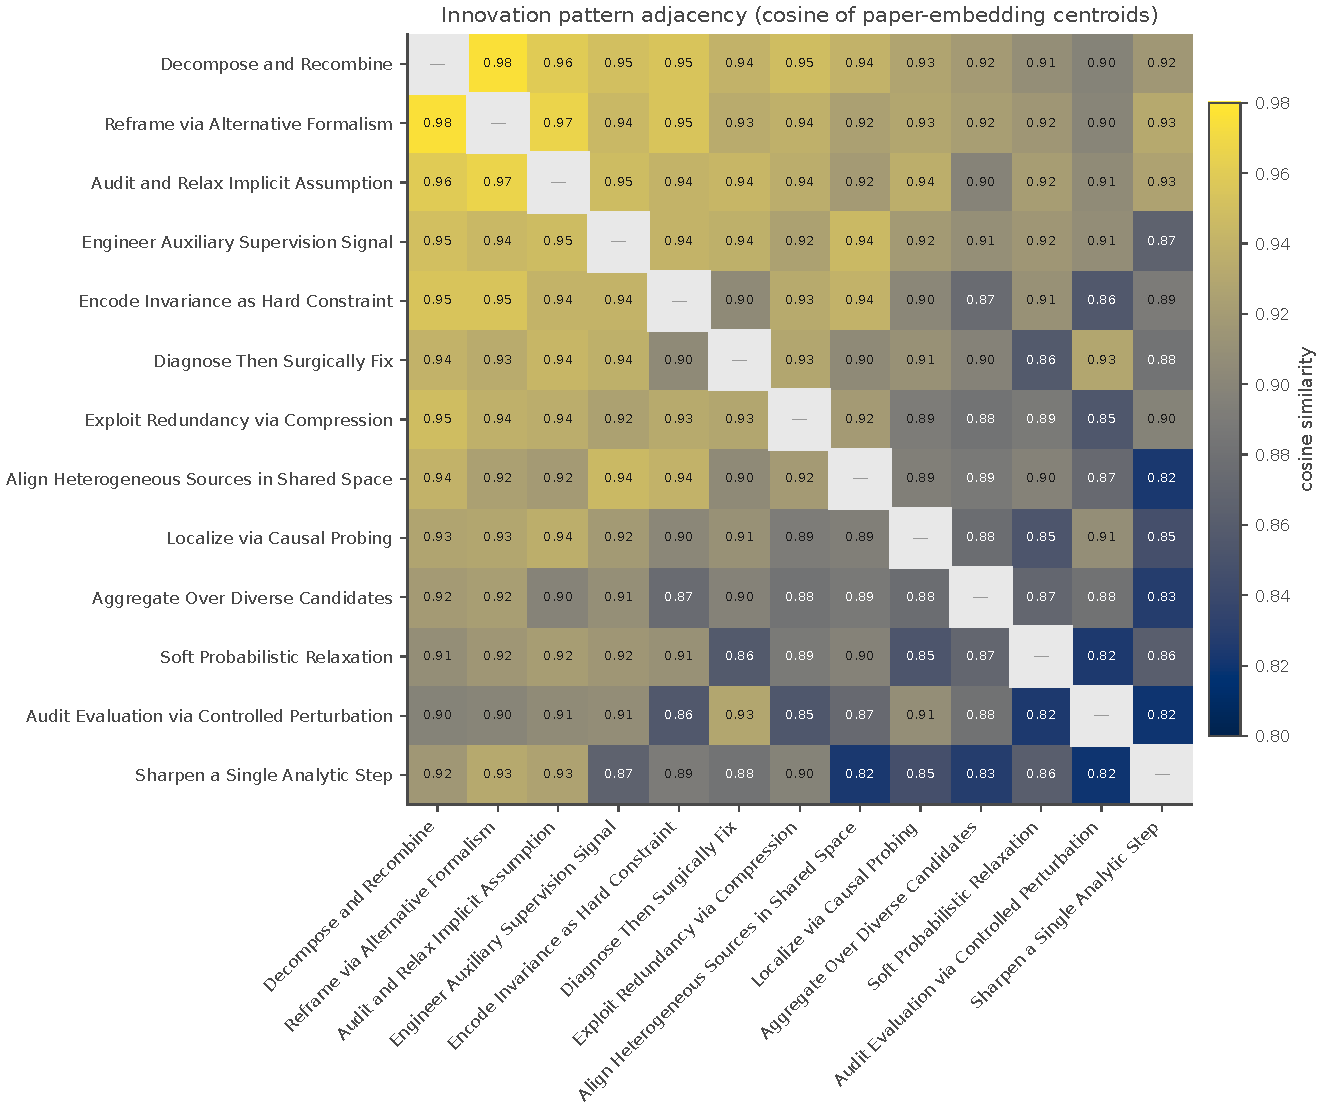
\includegraphics[width=0.92\textwidth]{figures/fig_methodology_adjacency.pdf}
\caption{Centroid-cosine similarity between the 13 innovation patterns. Rows/columns ordered by mean similarity (most ``central'' innovation patterns first). All off-diagonal entries fall in $[0.78, 0.98]$: innovation patterns are not orthogonal in this embedding, they form a dense neighborhood on a low-dimensional manifold.}
\label{fig:adjacency}
\end{figure}

\begin{table}[htbp]
\centering
\caption{Nearest-neighbor innovation pattern and centroid cosine. The neighbors corroborate the structure of Table~\ref{tab:combos}: the high-cosine pairs are exactly the ones that compose into Oral-favored combinations, and the most isolated innovation patterns (\emph{Aggregate Over Diverse Candidates}, \emph{Soft Probabilistic Relaxation}) are the small Reject-favored tail.}
\label{tab:nn}
\small
\begin{tabular}{p{6.0cm} p{6.0cm} r r}
\toprule
\textbf{Methodology} & \textbf{Nearest Neighbor} & \textbf{cosine} & \textbf{n} \\
\midrule
Reframe via Alternative Formalism & Decompose and Recombine & 0.975 & 259 \\
Decompose and Recombine & Reframe via Alternative Formalism & 0.975 & 68 \\
Audit and Relax Implicit Assumption & Reframe via Alternative Formalism & 0.966 & 250 \\
Encode Invariance as Hard Constraint & Decompose and Recombine & 0.955 & 101 \\
Engineer Auxiliary Supervision Signal & Decompose and Recombine & 0.950 & 54 \\
Exploit Redundancy via Compression & Decompose and Recombine & 0.949 & 69 \\
Align Heterogeneous Sources in Shared Space & Engineer Auxiliary Supervision Signal & 0.945 & 115 \\
Diagnose Then Surgically Fix & Audit and Relax Implicit Assumption & 0.943 & 95 \\
Localize via Causal Probing & Audit and Relax Implicit Assumption & 0.936 & 53 \\
Sharpen a Single Analytic Step & Reframe via Alternative Formalism & 0.932 & 93 \\
Audit Evaluation via Controlled Perturbation & Diagnose Then Surgically Fix & 0.929 & 93 \\
Aggregate Over Diverse Candidates & Reframe via Alternative Formalism & 0.922 & 11 \\
Soft Probabilistic Relaxation & Audit and Relax Implicit Assumption & 0.922 & 15 \\
\bottomrule
\end{tabular}
\end{table}

Three observations.

\textbf{(i) Adjacency predicts the Oral-favored combinations.} The four Oral-favored pairs in Table~\ref{tab:combos} (top) are all between high-cosine neighbors: \emph{analytic refinement}--\emph{audit} ($\cos\!\to\!0.932$ for sharpen$\to$reframe; nearby), \emph{audit}--\emph{reframing} (0.966), \emph{invariance}--\emph{shared latent} (0.945 via auxiliary signal hub), \emph{decomposition}--\emph{reframing} (0.975). Geometric proximity in the abstract$_*$ embedding is a useful priors signal for ``which secondary is plausible to compose with this primary''.

\textbf{(ii) The two most isolated innovation patterns are the two smallest and most Reject-prone.} \emph{Aggregate Over Diverse Candidates} ($n{=}11$) and \emph{Soft Probabilistic Relaxation} ($n{=}15$) have the lowest nearest-neighbor cosine (both 0.922) and also the worst $\Delta_{OR}$ profile in \S\ref{sec:analysis}. Embedding isolation, small sample, and Reject-skew co-occur --- consistent with these being genuinely rare strategies that the field has not yet learned to execute.

\textbf{(iii) The hub innovation patterns are framing-level.} \emph{Reframe via Alternative Formalism} appears as nearest neighbor for 6 of the other 12 innovation patterns, and \emph{Decompose and Recombine} for 4. This matches the structural reading of Table~\ref{tab:combos}: framing innovation patterns are the connective tissue of multi-strategy papers; an idea generator can usefully default to ``compose this execution innovation pattern with reframing or decomposition'' when no specific secondary is suggested by the query.

\subsection{Paper-level multi-label innovation pattern assignment}
\label{subsec:multilabel}

The cluster-level mapping in \S\ref{sec:methodology} caps at \emph{primary~+~secondary} per cluster (and therefore per paper). To verify that 2 is the right cap and to surface 3+ pattern combinations directly, we run a separate Opus~4.7 pass on every paper independently: given the 13 innovation pattern definitions and the paper's title, abstract, and four \texttt{abstract}$_*$ fields, the model emits a JSON list of innovation patterns the paper actually \emph{executes} (not just mentions), each with a quoted evidence span and a \texttt{primary}/\texttt{supporting} role. There is no upper cap on \(k = |\text{applied\_methodologies}|\); the minimum is~1.

All 1{,}947 papers received a non-empty assignment. Rather than report a Bayesian acceptance rate (which requires constructing a denominator that mixes the OpenReview Oral/Reject decision with the citation-based HC class — these classes overlap in reality and we bucket exclusively into Oral $\succ$ HC $\succ$ Reject), we report the \emph{class-conditional distribution} \(P(k \mid \text{decision})\) directly. Table~\ref{tab:k_dist} shows, within each acceptance class, what fraction of that class's papers execute \(k\) innovation patterns.

\begin{table}[htbp]
\centering
\caption{Class-conditional \(k\) distribution. Each column sums to 100\% within its class. \(\bar{k}\) is the per-class mean. Cells are \(n\) (\%-of-class).}
\label{tab:k_dist}
\small
\begin{tabular}{c r r r r}
\toprule
\(k\) & all (n=1947) & Oral (n=1014) & HC (n=211) & Reject (n=722) \\
\midrule
1 &   47 (2.4\%) &  22 (2.2\%) &   3 (1.4\%) &  22 (3.1\%) \\
2 &  630 (32.4\%) & 318 (31.3\%) &  60 (28.4\%) & 252 (35.0\%) \\
3 & \textbf{1116 (57.3\%)} & \textbf{604 (59.4\%)} & \textbf{124 (58.8\%)} & \textbf{388 (53.9\%)} \\
4 &  149 (7.7\%) &  70 (6.9\%) &  \textbf{23 (10.9\%)} &  56 (7.8\%) \\
5 &    5 (0.3\%) &   2 (0.2\%) &   1 (0.5\%) &   2 (0.3\%) \\
\midrule
\(\bar{k}\) & 2.71 & 2.72 & \textbf{2.81} & 2.67 \\
\bottomrule
\end{tabular}
\end{table}

Three observations.

\textbf{(i) \(k{=}3\) is the empirical mode in every class.} 57.3\% of all papers execute exactly three innovation patterns. The mode is shared across Oral (59.4\%), HC (58.8\%), and Reject (53.9\%). The cluster-based view of \S\ref{subsec:multistrat} (which capped at \(k=2\) by construction) systematically under-counted: 67.6\% of papers have \(k \geq 3\) but were forced into a \(k \leq 2\) view by the cluster mapping. Paper-level multi-label is the right granularity for capturing this.

\textbf{(ii) HC papers are slightly more complex than Oral, which are slightly more complex than Reject.} The class means are tightly stacked: \(\bar{k}_R = 2.67 < \bar{k}_O = 2.72 < \bar{k}_{HC} = 2.81\). The \(\bar{k}_{HC} - \bar{k}_O = 0.09\) gap is small but driven entirely by the \(k{=}4\) tail: 10.9\% of HC papers have \(k=4\), versus 6.9\% of Oral and 7.8\% of Reject — HC papers are \(1.58\times\) more likely to be at \(k=4\) than Oral. The 23 HC papers at \(k{=}4\) consistently include \emph{Engineer Auxiliary Supervision Signal} as one of the four (a innovation pattern that is mildly Reject-favored in 2-way combinations, \S\ref{subsec:multistrat}), suggesting HC papers buy citation persistence by composing comprehensive innovation pattern stacks where Oral papers stop at three.

\textbf{(iii) Cluster-based pair grossly under-represents true innovation pattern coverage.} Cross-tabulating against the cluster-derived \texttt{(primary, secondary)} pair: the cluster primary is present in the paper-level set \emph{only} 64.3\% of the time, the cluster secondary 53.1\% of the time, and \textbf{1860 of 1947 papers (95.6\%) have at least one innovation pattern beyond the cluster pair}. The cluster pair is not wrong, but it captures only the dominant axis. Multi-label tagging surfaces the routine 1--2 supporting moves that distinguish Oral execution.

\begin{figure}[htbp]
\centering
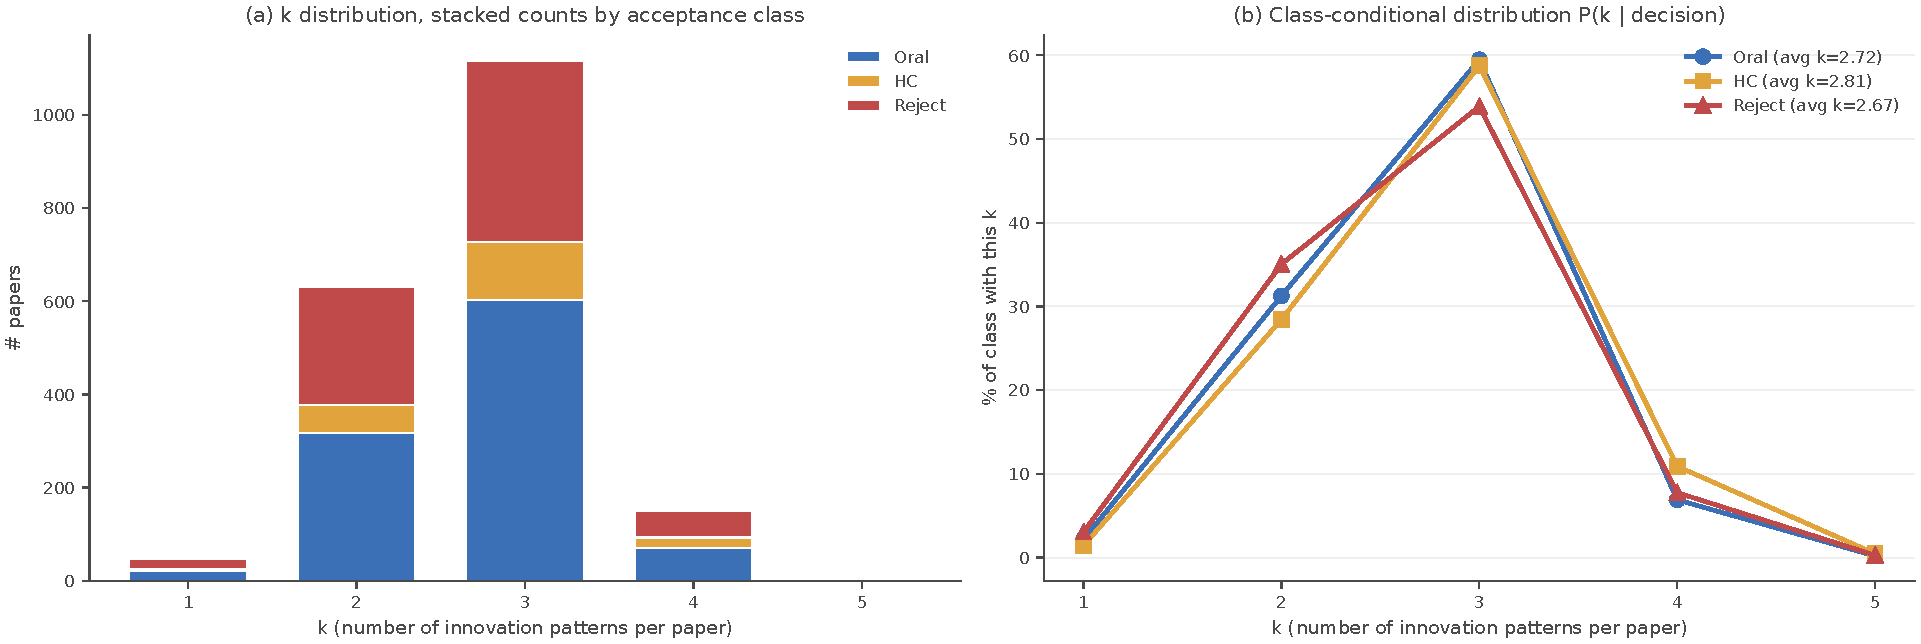
\includegraphics[width=\textwidth]{figures/fig_multilabel_k.pdf}
\caption{Multi-label innovation pattern assignment. (a)~\(k\) distribution as stacked counts by acceptance class. (b)~Class-conditional distribution \(P(k \mid \text{decision})\): each curve is a probability mass function summing to 100\%. \(k{=}3\) is the mode for all three classes; HC has a heavier \(k{=}4\) tail (10.9\%) than Oral (6.9\%) or Reject (7.8\%).}
\label{fig:multilabel_k}
\end{figure}

\paragraph{Multi-label coverage of HDBSCAN-unclustered papers.} The paper-level multi-label tagging is independent of HDBSCAN. We therefore use it to verify what the unclustered label means. Table~\ref{tab:unclustered_vs_clustered} shows the comparison: unclustered and clustered papers carry near-identical innovation pattern compositions, and unclustered papers actually have a slightly higher Oral rate. The HDBSCAN-unclustered label is therefore not a measure of strategic emptiness; it is a measure of \emph{embedding-geometry typicality} (whether a paper's specific phrasing places it inside a modal cluster's density region). The three-pattern composition that defines the empirical mode is just as common in unclustered as in clustered --- unclustered papers do not lack innovation pattern composition, they lack \emph{modal} composition.

\begin{table}[htbp]
\centering
\caption{HDBSCAN-unclustered vs.\ clustered papers under independent paper-level multi-label tagging. The two groups are statistically indistinguishable on innovation pattern composition; unclustered papers are slightly more Oral-favored.}
\label{tab:unclustered_vs_clustered}
\small
\begin{tabular}{l r r}
\toprule
& unclustered (n=671) & clustered (n=1276) \\
\midrule
mean $k$                                 & 2.75    & 2.69    \\
$k=1$                                    & 2.1\%   & 2.6\%   \\
$k=2$                                    & 31.3\%  & 32.9\%  \\
$k=3$ (modal)                            & 56.8\%  & 57.6\%  \\
$k=4$                                    & \textbf{9.7\%}   & 6.6\%   \\
$k=5$                                    & 0.1\%   & 0.3\%   \\
\midrule
Oral rate                                & \textbf{54.8\%}  & 50.8\%  \\
HC rate                                  & 9.7\%   & 11.4\%  \\
Reject rate                              & 35.5\%  & 37.8\%  \\
\midrule
all 4 \texttt{abstract\_*} fields populated & 100\%   & 100\%   \\
median \texttt{abstract\_strategy} length   & 218 chars & 220 chars \\
\bottomrule
\end{tabular}
\end{table}

The slightly elevated $k{=}4$ tail in unclustered (9.7\% vs.\ 6.6\%) is consistent with the geometric reading: papers that execute four innovation patterns with comparable weight are more likely to land between modal clusters than papers with a sharply dominant primary innovation pattern. ``Between modal clusters'' is also where some of the most-novel ideas live --- atypical-execution papers are over-represented in the unclustered group's Oral rate.

\paragraph{Top combinations under multi-label tagging.}
With paper-level multi-label assignments we rank 2-way and 3-way combinations directly (Table~\ref{tab:multilabel_combos}), reporting the class-conditional distribution \((\%_O, \%_{HC}, \%_R)\) within each combination's papers rather than a constructed Bayesian rate. Sample sizes are much larger than under the cluster-pair view (e.g.\ \emph{audit~+~reframe} appears in 538 papers under multi-label vs 137 under cluster-pair). The standout 3-way result: \emph{audit~+~reframe~+~shared\_latent\_alignment} carries \(n=18\) papers split 12/6/0 — \textbf{67\% Oral, 33\% HC, 0\% Reject} — the only combination at \(n \geq 10\) where every paper is in an accepted class. Its presence in 6 of our 211 HC papers as well makes it doubly distinctive: high-acceptance and high-citation simultaneously.

\begin{table}[htbp]
\centering
\caption{Top innovation pattern combinations under multi-label tagging, ranked by lowest Reject share within the combination's papers. Each row is a combination's class-conditional distribution: \(\%_O = n_O/n\), \(\%_{HC} = n_{HC}/n\), \(\%_R = n_R/n\) (rows sum to 100\%). 2-way threshold \(n \geq 20\); 3-way threshold \(n \geq 10\). Compare with Table~\ref{tab:combos} (cluster-based, capped at pair).}
\label{tab:multilabel_combos}
\small
\begin{tabular}{p{8.4cm} r r r r r r}
\toprule
\textbf{Combination} & \(n\) & \(n_O\) & \(n_{HC}\) & \(n_R\) & \(\%_O / \%_{HC} / \%_R\) \\
\midrule
\multicolumn{6}{l}{\textit{Top 2-way (n \(\geq\) 20), sorted by lowest \%-reject}} \\
\midrule
\textit{eval audit} + \textit{causal probing}                                   &  42 &  28 &  9 &   5 & 67/21/\textbf{12} \\
\textit{sharpen analytic} + \textit{reframing}                                  &  87 &  70 &  0 &  17 & 80/0/20 \\
\textit{causal probing} + \textit{surgical fix}                                 &  35 &  22 &  6 &   7 & 63/17/20 \\
\textit{sharpen analytic} + \textit{decompose}                                  &  43 &  32 &  1 &  10 & 74/2/23 \\
\textit{reframing} + \textit{shared latent alignment}                           &  54 &  32 &  9 &  13 & 59/17/24 \\
\textit{aggregate over diverse} + \textit{reframing}                            &  32 &  21 &  3 &   8 & 66/9/25 \\
\textit{sharpen analytic} + \textit{surgical fix}                               &  44 &  31 &  2 &  11 & 70/5/25 \\
\textit{audit} + \textit{reframing}                                             & 538 & 345 & 45 & 148 & 64/8/28 \\
\textit{eval audit} + \textit{surgical fix}                                     &  36 &  21 &  5 &  10 & 58/14/28 \\
\textit{eval audit} + \textit{reframing}                                        &  47 &  27 &  6 &  14 & 57/13/30 \\
\midrule
\multicolumn{6}{l}{\textit{Top 3-way (n \(\geq\) 10), sorted by lowest \%-reject}} \\
\midrule
\textbf{\textit{audit} + \textit{reframing} + \textit{shared latent alignment}} &  \textbf{18} &  \textbf{12} &   \textbf{6} &   \textbf{0} & \textbf{67/33/0} \\
\textit{sharpen analytic} + \textit{audit} + \textit{reframing}                 &  49 &  42 &  0 &   7 & 86/0/14 \\
\textit{audit} + \textit{reframing} + \textit{redundancy compression}           &  26 &  19 &  3 &   4 & 73/12/15 \\
\textit{decompose} + \textit{reframing} + \textit{shared latent alignment}      &  12 &   9 &  1 &   2 & 75/8/17 \\
\textit{audit} + \textit{causal probing} + \textit{surgical fix}                &  10 &   5 &  3 &   2 & 50/30/20 \\
\textit{audit} + \textit{eval audit} + \textit{surgical fix}                    &  15 &  10 &  2 &   3 & 67/13/20 \\
\textit{audit} + \textit{eval audit} + \textit{causal probing}                  &  19 &  12 &  3 &   4 & 63/16/21 \\
\textit{audit} + \textit{reframing} + \textit{invariance constraint}            &  43 &  31 &  2 &  10 & 72/5/23 \\
\textit{sharpen analytic} + \textit{decompose} + \textit{reframing}             &  17 &  13 &  0 &   4 & 76/0/24 \\
\textit{decompose} + \textit{reframing} + \textit{soft probabilistic}           &  16 &  11 &  1 &   4 & 69/6/25 \\
\bottomrule
\end{tabular}
\end{table}

\paragraph{What multi-label tagging implies for the SKILL.} The SKILL system treats innovation-pattern composition as 1--3 entries per generated idea (with \(k = 3\) as the empirically supported default), drawing from the innovation pattern cards (\S\ref{subsec:cards}) for the success/failure conditions of each composed innovation pattern. The combination statistics in Table~\ref{tab:multilabel_combos} are surfaced informationally --- not as generation priors --- via the candidate's \texttt{innovation\_pattern\_landscape} block, which echoes the area's pattern usage alongside the candidate's chosen composition so the user sees where their idea sits in the empirical distribution. Selection of patterns happens upstream by structural fit to the bottleneck (Phase 2.1), not by composition-rate priors; loading priors at generation time was tested in an earlier design and removed because it induced distribution-bias homogenization across runs. The 100\%-Oral combination \emph{audit + reframing + shared\_latent\_alignment} is therefore reported here as an empirical observation, not as a SKILL target template.


%======================================================================
\section{Acceptance and Impact Analysis}
\label{sec:analysis}
%======================================================================

\subsection{Oral-vs-Reject bias per innovation pattern}

We define the acceptance bias $\Delta_{\text{OR}}(m) = p_\text{oral}(m) - p_\text{reject}(m)$, where $p_\text{oral}(m)$ is the fraction of Oral papers whose primary innovation pattern is $m$ and $p_\text{reject}(m)$ is analogous for Reject. Positive $\Delta_{\text{OR}}$ means reviewers reward the innovation pattern relative to its baseline rejection rate; negative means the innovation pattern appears in rejected work more than in accepted work, relative to totals. Figure~\ref{fig:bias} plots the bias for all 13 innovation patterns; Table~\ref{tab:bias} gives the numbers.

\begin{table}[htbp]
\centering
\caption{Per-innovation pattern acceptance bias. \(p_\text{oral}\) is the fraction of all Oral papers ($N{=}1{,}014$) whose primary is this innovation pattern; \(p_\text{reject}\) is analogous among Reject ($N{=}722$). $\Delta_{\text{OR}}{=}p_\text{oral}-p_\text{reject}$ in pp. $\Delta_{\text{OH}}{=}p_\text{oral}-p_\text{hc}$ (positive = PC-favored over community).}
\label{tab:bias}
\small
\begin{tabular}{p{6.5cm} rrrrr}
\toprule
\textbf{Methodology} & \(p_\text{oral}\) & \(p_\text{hc}\) & \(p_\text{reject}\) & \(\Delta_{\text{OR}}\) & \(\Delta_{\text{OH}}\) \\
\midrule
Reframe via Alternative Formalism & 15.9 & 8.1 & 11.8 & \textbf{+4.2} & +7.9 \\
Audit Evaluation via Controlled Perturbation & 4.5 & 11.2 & 3.0 & +1.5 & $-$6.6 \\
Sharpen a Single Analytic Step & 5.9 & 0.4 & 4.6 & +1.3 & +5.5 \\
Encode Invariance as Hard Constraint & 6.1 & 1.9 & 5.0 & +1.1 & +4.2 \\
Aggregate Over Diverse Candidates & 0.6 & 1.2 & 0.4 & +0.2 & $-$0.6 \\
Localize via Causal Probing & 2.9 & 2.3 & 2.8 & +0.1 & +0.5 \\
Exploit Redundancy via Compression & 3.1 & 5.0 & 4.0 & $-$1.0 & $-$1.9 \\
Diagnose Then Surgically Fix & 2.8 & 18.1 & 3.7 & $-$1.0 & \textbf{$-$15.3} \\
Engineer Auxiliary Supervision Signal & 2.3 & 3.5 & 3.3 & $-$1.1 & $-$1.2 \\
Soft Probabilistic Relaxation & 0.3 & 0.0 & 1.7 & $-$1.4 & +0.3 \\
Decompose and Recombine & 3.1 & 1.9 & 4.4 & $-$1.4 & +1.1 \\
Align Heterogeneous Sources in Shared Space & 4.4 & 8.5 & 7.2 & $-$2.8 & $-$4.0 \\
Audit and Relax Implicit Assumption & 12.0 & 8.8 & 15.0 & \textbf{$-$3.0} & +3.2 \\
\bottomrule
\end{tabular}
\end{table}

\begin{figure}[htbp]
\centering
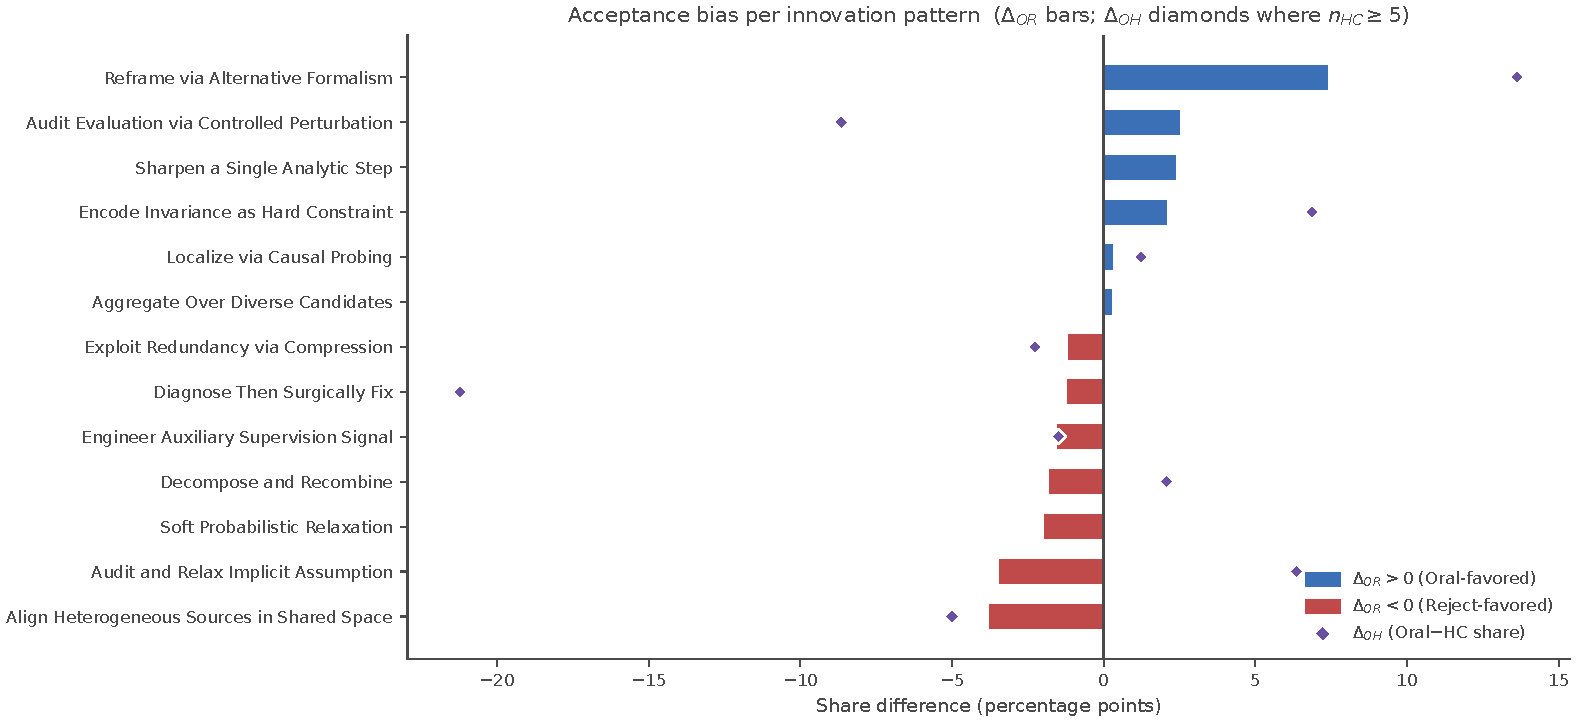
\includegraphics[width=0.95\textwidth]{figures/fig_methodology_bias.pdf}
\caption{Per-innovation pattern Oral vs Reject shares (pp). Methodologies above the diagonal are Oral-favored; below are Reject-over-represented.}
\label{fig:bias}
\end{figure}

Four observations follow.

\textbf{(O1)} \emph{Formal reframing} is the single most PC-favored innovation pattern in absolute terms: it accounts for 162 Oral papers---more than any other innovation pattern---and $\Delta_{\text{OR}}{=}{+}4.2$ pp. Combined with the fact that it pairs most often with \emph{assumption audit} (Table~\ref{tab:combos}), the data suggests a recipe: re-derive a standard problem in a different formalism, then use that formalism to attack an assumption that the original formalism hid.

\textbf{(O2)} \emph{Assumption audit} is high-volume but high-variance: $p_\text{oral}{=}12.0\%$ and $p_\text{reject}{=}15.0\%$ (the highest Reject share of any innovation pattern), giving $\Delta_{\text{OR}}{=}{-}3.0$. Relaxing an assumption is the second-largest route to Oral in absolute terms (122 papers), but it is also the most common route to Reject (108 papers). Execution-level quality, not strategy choice, is what separates the two pools within this innovation pattern.

\textbf{(O3)} \emph{Shared latent alignment} is structurally risky: it is the only innovation pattern in the top six by Reject count that simultaneously has a mid-single-digit Oral share. Its $\Delta_{\text{OR}}$ of $-2.8$ pp and $\Delta_{\text{OH}}$ of $-4.0$ pp both point in the ``looks like alignment-via-representation-sharing'' direction reviewers flag as incremental.

\textbf{(O4)} \emph{Soft probabilistic relaxation} has the smallest absolute sample (15 papers) but the clearest bias: 3 Oral vs 12 Reject. Although underpowered, it is consistent with the folk claim that ``make it soft'' is often a surface-level move without deeper structural justification.

\subsection{PC-vs-community bias ($\Delta_{\text{OH}}$)}

The \(\Delta_{\text{OH}}{=}p_\text{oral}-p_\text{hc}\) column of Table~\ref{tab:bias} isolates the second, orthogonal axis: are program committees and the citing community aligned on what counts? Two innovation patterns stand out.

\textbf{\emph{Diagnose Then Surgically Fix}}: $\Delta_{\text{OH}}{=}{-}15.3$ pp is the largest anti-Oral skew in the taxonomy. These papers (28 Oral, 47 HC) isolate a specific pathology and deploy a minimal targeted fix that gets reproduced and cited, but program committees judge the contribution as narrow. Every strong practitioner knows this pattern: if your paper is ``we noticed X and fixed it by doing Y,'' the community will cite you but the PC may not call it Oral.

\textbf{\emph{Sharpen a Single Analytic Step}}: $\Delta_{\text{OH}}{=}{+}5.5$ pp with only one HC paper (out of 260) but 60 Oral papers. Proof-tightening work is consistently PC-rewarded and consistently uncited. This is the cleanest PC-bias signal in the taxonomy.

\textbf{\emph{Audit Evaluation via Controlled Perturbation}} is the mirror: $\Delta_{\text{OH}}{=}{-}6.6$ pp, driven by 29 HC vs 46 Oral---a near-parity that, adjusted for pool sizes, makes it the single most \emph{community-favored} innovation pattern. Our data suggests this is the rising innovation pattern of 2024--2025 (see temporal analysis below).

\paragraph{An alternative, conditional-on-accepted PC-bias cut.} The $\Delta_{\text{OH}}$ above measures absolute population-level skew (Oral rate minus HC rate of all papers, including reject). A complementary cut conditions on the accepted pool: \emph{Bias} $= p_\text{oral|accepted} - p_\text{hc|accepted}$, the share of Oral within Oral~$+$~HC per innovation pattern. This answers a different question --- ``among papers that the community already validated as accepted, what fraction did program committees additionally elevate?'' --- and yields the four-bucket type classification in Table~\ref{tab:pc-bias-types}. We surface this table for analytic transparency; the SKILL itself does not consume PC-bias buckets at any phase, to avoid re-introducing distribution-bias homogenization (every run drifting toward Strong-PC patterns regardless of the user's bottleneck).

\begin{table}[htbp]
\centering
\caption{Per-methodology PC bias categorization for the SKILL's reviewer simulation. \emph{Bias} $= p_\text{oral|accepted} - p_\text{hc|accepted}$. Type bucket: \emph{Strong PC} $> 0.6$, \emph{Moderate PC} $0.3$--$0.6$, \emph{Balanced} $-0.1$--$0.3$, \emph{Community} $\leq -0.1$.}
\label{tab:pc-bias-types}
\small
\begin{tabular}{p{5.4cm} rrr rr l}
\toprule
\textbf{Methodology} & $n$ & $n_O$ & $n_H$ & \textbf{Oral\%} & \textbf{HC\%} & \textbf{Type} \\
\midrule
Sharpen a Single Analytic Step & 260 & 60 & 1 & 96.6 & 3.4 & Strong PC \\
Reframe via Alternative Formalism & 657 & 156 & 26 & 85.6 & 14.4 & Strong PC \\
Encode Invariance as Hard Constraint & 197 & 88 & 16 & 84.6 & 15.4 & Strong PC \\
Soft Probabilistic Relaxation &  85 & 49 &  9 & 84.5 & 15.5 & Strong PC \\
Audit and Relax Implicit Assumption & 988 & 245 & 61 & 80.1 & 19.9 & Strong PC \\
Diagnose Then Surgically Fix & 391 & 87 & 27 & 76.3 & 23.7 & Moderate PC \\
Aggregate Over Diverse Candidates &  62 & 29 &  9 & 76.3 & 23.7 & Moderate PC \\
Decompose and Recombine & 391 & 95 & 30 & 76.0 & 24.0 & Moderate PC \\
Localize via Causal Probing & 116 & 53 & 19 & 73.6 & 26.4 & Moderate PC \\
Engineer Auxiliary Supervision Signal & 350 & 60 & 22 & 73.2 & 26.8 & Moderate PC \\
Exploit Redundancy via Compression & 251 & 65 & 25 & 72.2 & 27.8 & Moderate PC \\
Align Heterogeneous Sources in Shared Space & 339 & 71 & 30 & 70.3 & 29.7 & Moderate PC \\
Audit Evaluation via Controlled Perturbation & 197 & 81 & 40 & 66.9 & 33.1 & Moderate PC \\
\bottomrule
\end{tabular}
\end{table}

In our 1947-paper corpus, no innovation pattern lands in the \emph{Balanced} or \emph{Community} buckets: every innovation pattern in the taxonomy is at least Moderate PC. This is itself a structural finding --- across the post-2020 ICLR/ICML/NeurIPS pool, the venues' Oral selection is consistently more reviewer-favored than the citing community would predict, and the bias is sharpest for theory-anchored innovation patterns (\emph{Sharpen a Single Analytic Step}, $+0.93$; \emph{Reframe via Alternative Formalism}, $+0.71$; \emph{Encode Invariance as Hard Constraint}, $+0.69$). The SKILL's R0 advocate is required to read this table and, when the candidate's anchor lens has Bias $> 0.6$, name the specific durability mechanism that lifts the candidate above the typical PC-favored fate; meta-(b) likewise must report the Best-Paper gap in PC-bias-aware terms ('the further gap is durability mechanism X', not 'the further gap is X' generically).


%======================================================================
\section{Domain Distribution and Methodology Breadth}
\label{sec:domains}
%======================================================================

The innovation pattern cards (\S\ref{subsec:cards}) and the per-pattern bias profile (\S\ref{sec:analysis}) treat the 1{,}947 papers as a single population. But ML is not a monolithic field: a strategy that lands an Oral in \emph{learning theory} may not land in \emph{vision-language pretraining}, and the SKILL needs to know which innovation patterns are domain-agnostic versus domain-specific. This section quantifies that.

\subsection{Domain induction}
\label{subsec:domain-induction}

We do not preset a domain taxonomy. Instead, we induce one from the data using the same architecture that produced the 13 innovation patterns: (1) Sonnet extracts 1--3 normalized research-subarea tags per paper from its title, abstract, and (when available, $77.9\%$ of the dataset) author-supplied OpenReview keywords; (2) the 3{,}909 unique free-form tags are embedded with OpenAI \texttt{text-embedding-3-large} and clustered with UMAP+HDBSCAN ($k{=}148$ tag-clusters at $\textit{mcs}{=}7$, unclustered $25.5\%$); (3) Sonnet labels each tag-cluster; (4) Opus 4.7 induces a Level-1 domain taxonomy of $N \in [8, 30]$ entries and maps every tag-cluster to one domain. The model returns $N{=}28$ domains; we make no edits.

The per-paper assignment is the union of domains over each paper's tags. Coverage: $\mathbf{98.5\%}$ of papers (1{,}918 / 1{,}947) receive at least one domain; the average is $1.81$ domains per paper. The 28 domains range from $n{=}256$ (\textit{Transfer, Continual \& Meta-Learning}) down to $n{=}16$ (\textit{Online \& Bandit Learning}); the full ordered list and machine-readable taxonomy are in \texttt{clustering/domains/domain\_taxonomy.json}.

\subsection{Domain $\times$ innovation pattern heatmap}
\label{subsec:dm-heatmap}

Figure~\ref{fig:domain_method} shows two views of the $28 \times 13$ joint structure: panel (a) is the raw paper count per cell; panel (b) is the cell-level Oral rate $p_O = n_O / (n_O + n_R)$, masked where $n_O + n_R < 5$ to avoid spurious low-sample reads. 120 of the 364 cells (33\%) clear the $\geq 5$ threshold, yielding a dense-enough sub-matrix for cell-level conclusions.

\begin{figure}[htbp]
\centering
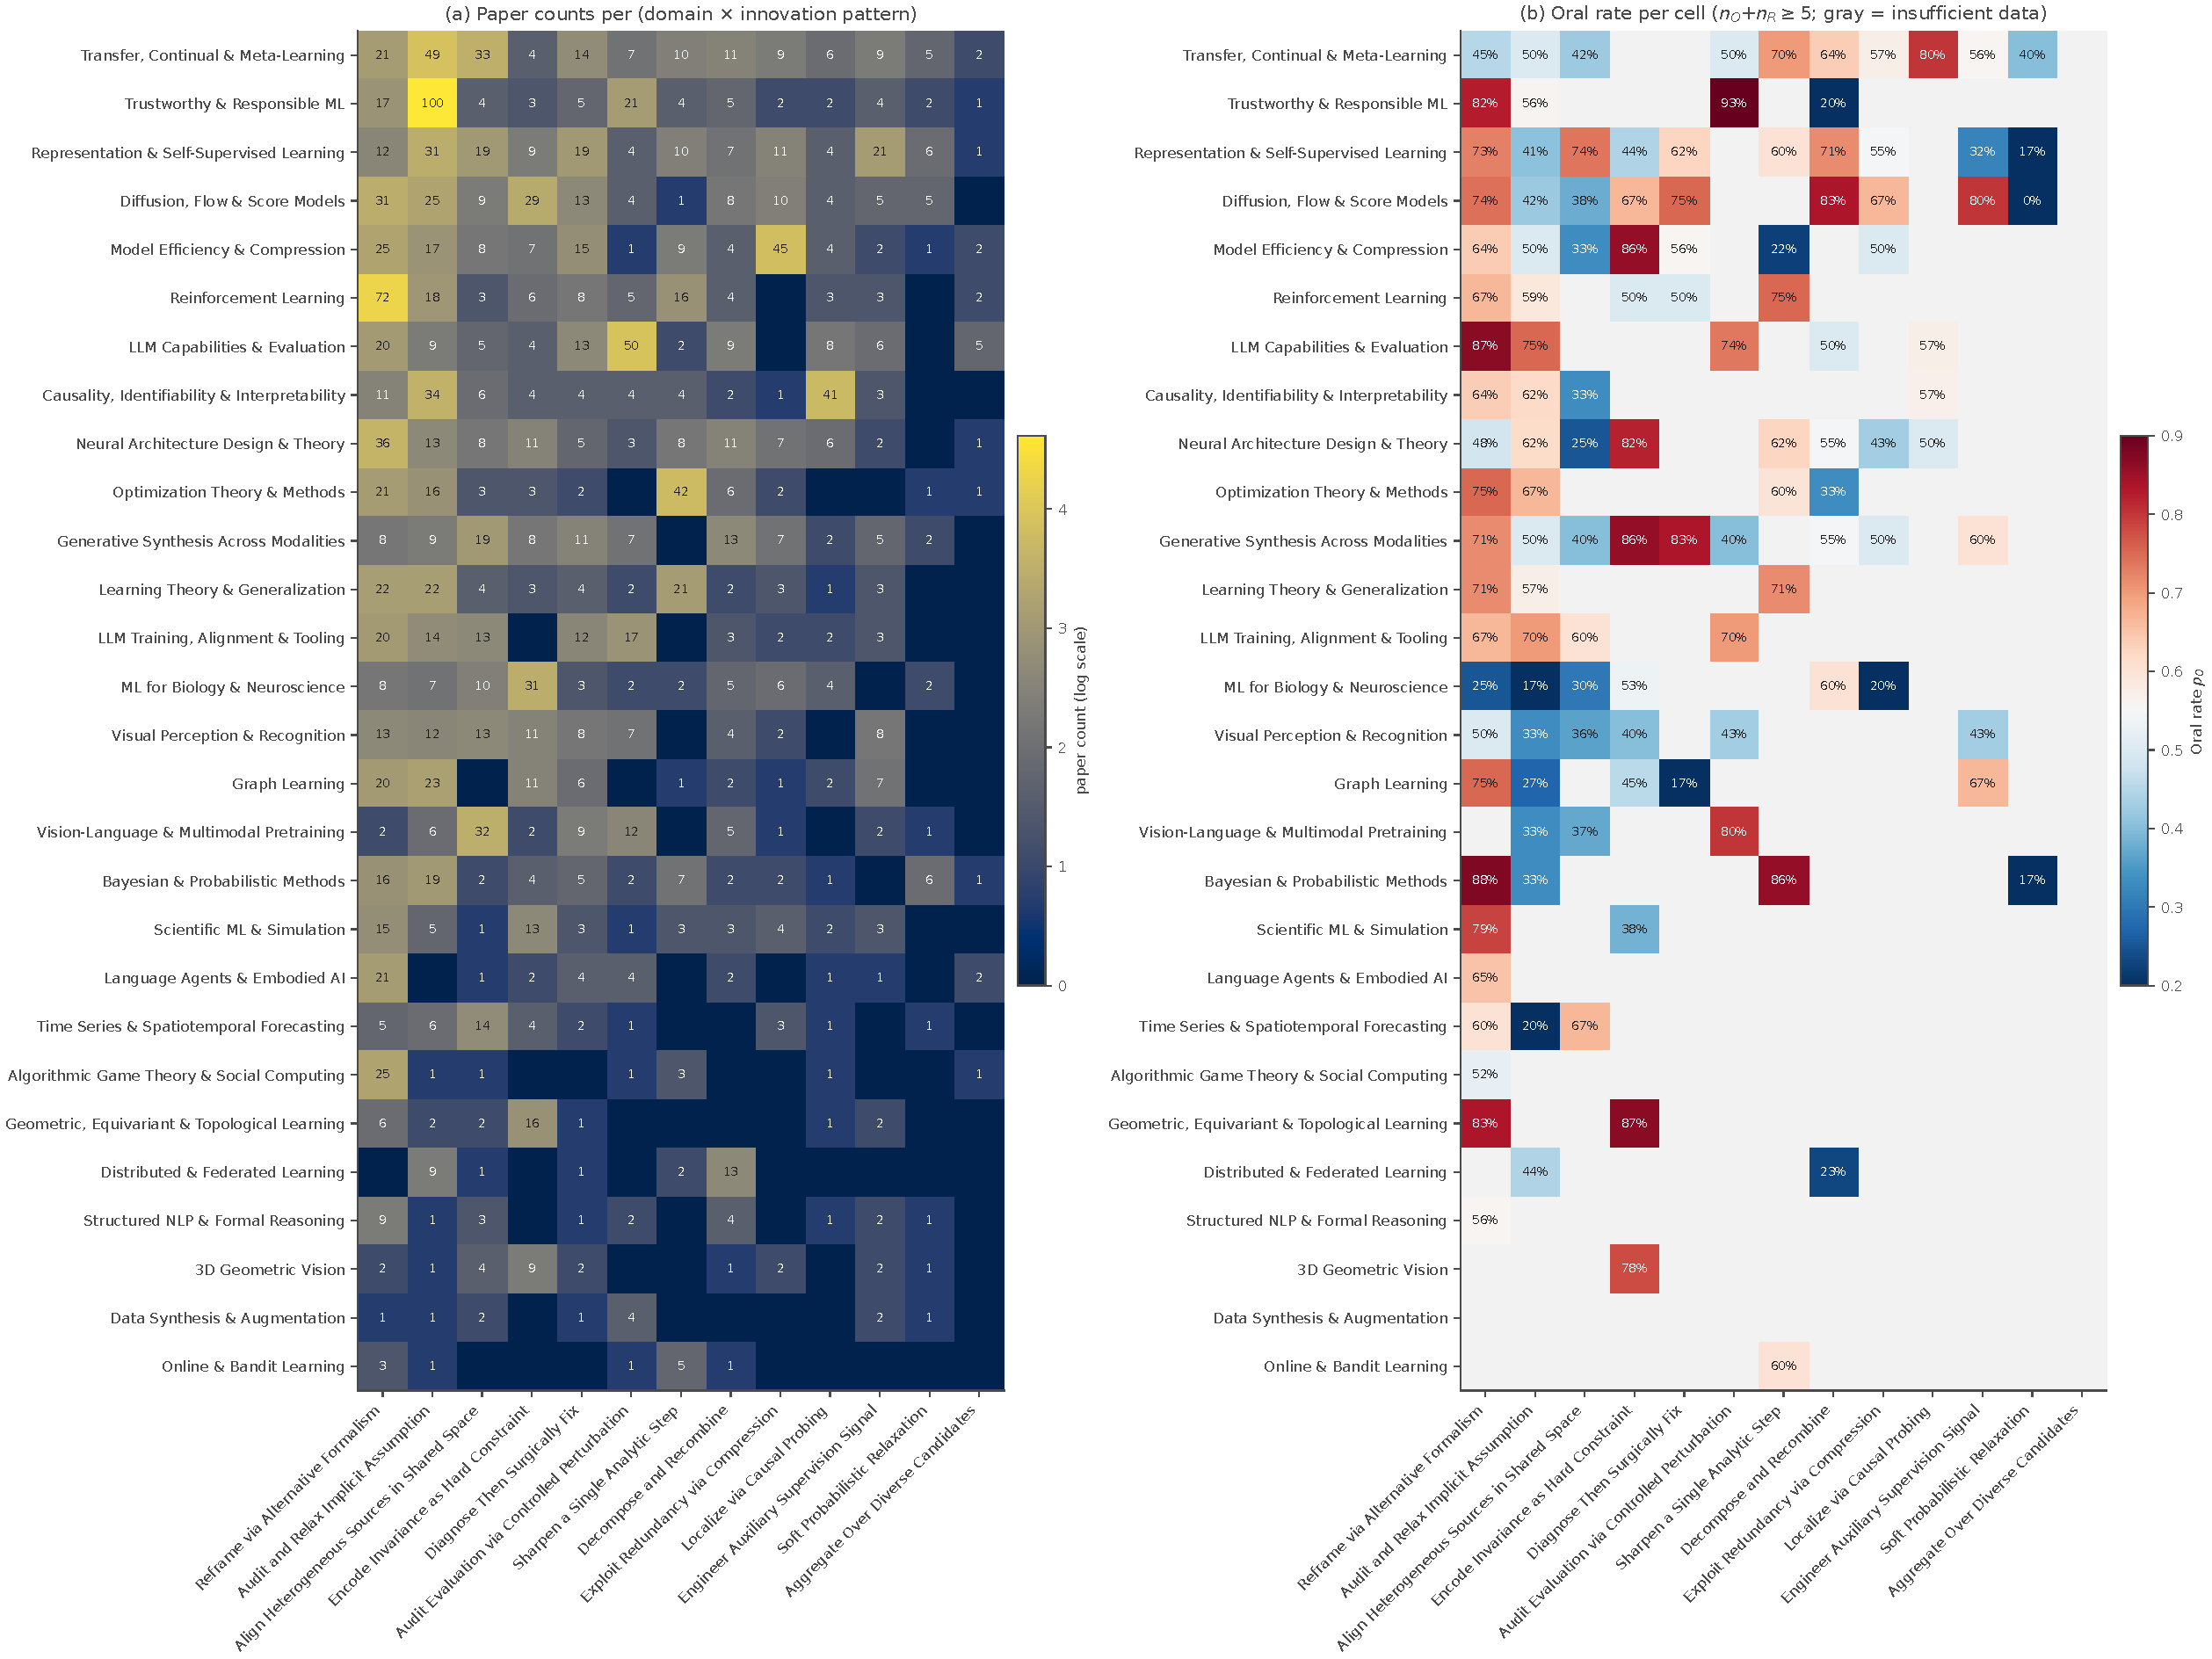
\includegraphics[width=\textwidth]{figures/fig_domain_methodology.pdf}
\caption{(a) Paper counts per (domain, innovation pattern) cell --- domains and innovation patterns sorted by total. (b) Per-cell Oral rate $p_O$ (cells with $n_O + n_R < 5$ are blank). The colored signal in (b) is heterogeneous: the same innovation pattern can land at $90\%$ Oral in one domain and $40\%$ Oral in another.}
\label{fig:domain_method}
\end{figure}

The cell-level reads confirm the high-level picture from \S\ref{sec:analysis} but add domain specificity. The strongest cells (each $p_O \geq 75\%$ on $n \geq 8$):

\begin{itemize}[leftmargin=1.4em, topsep=2pt, itemsep=2pt]
\item \textit{Trustworthy \& Responsible ML} $\times$ \textit{Audit Evaluation via Controlled Perturbation}: $\mathbf{93\%}$ Oral ($n_O{=}14$, $n_R{=}1$) --- the dataset's single highest-acceptance cell.
\item \textit{Bayesian \& Probabilistic Methods} $\times$ \textit{Reframe via Alternative Formalism}: $88\%$ ($14/2$).
\item \textit{LLM Capabilities \& Evaluation} $\times$ \textit{Reframe via Alternative Formalism}: $87\%$ ($13/2$).
\item \textit{Geometric, Equivariant \& Topological Learning} $\times$ \textit{Encode Invariance as Hard Constraint}: $87\%$ ($13/2$).
\item \textit{Neural Architecture Design \& Theory} $\times$ \textit{Encode Invariance as Hard Constraint}: $82\%$ ($9/2$).
\end{itemize}

The weakest cells ($p_O < 56\%$): \textit{Distributed \& Federated Learning} $\times$ \textit{Audit and Relax Implicit Assumption} ($44\%$); \textit{Visual Perception \& Recognition} $\times$ \textit{Reframe via Alternative Formalism} ($50\%$); \textit{Algorithmic Game Theory \& Social Computing} $\times$ \textit{Reframe via Alternative Formalism} ($52\%$); \textit{ML for Biology \& Neuroscience} $\times$ \textit{Encode Invariance as Hard Constraint} ($53\%$). The same innovation pattern that wins in adjacent domains under-performs here, consistent with the cards' guidance that the success conditions are not transparently transferable across domains.

\subsection{Methodology breadth: how domain-agnostic is each innovation pattern?}
\label{subsec:breadth}

For the SKILL system to make ``method X works in your domain'' recommendations, we need each methodology's domain footprint. Figure~\ref{fig:breadth} plots, for each innovation pattern, the number of distinct domains it touches (with at least one paper) and the share of its papers concentrated in its single largest domain.

\begin{figure}[htbp]
\centering
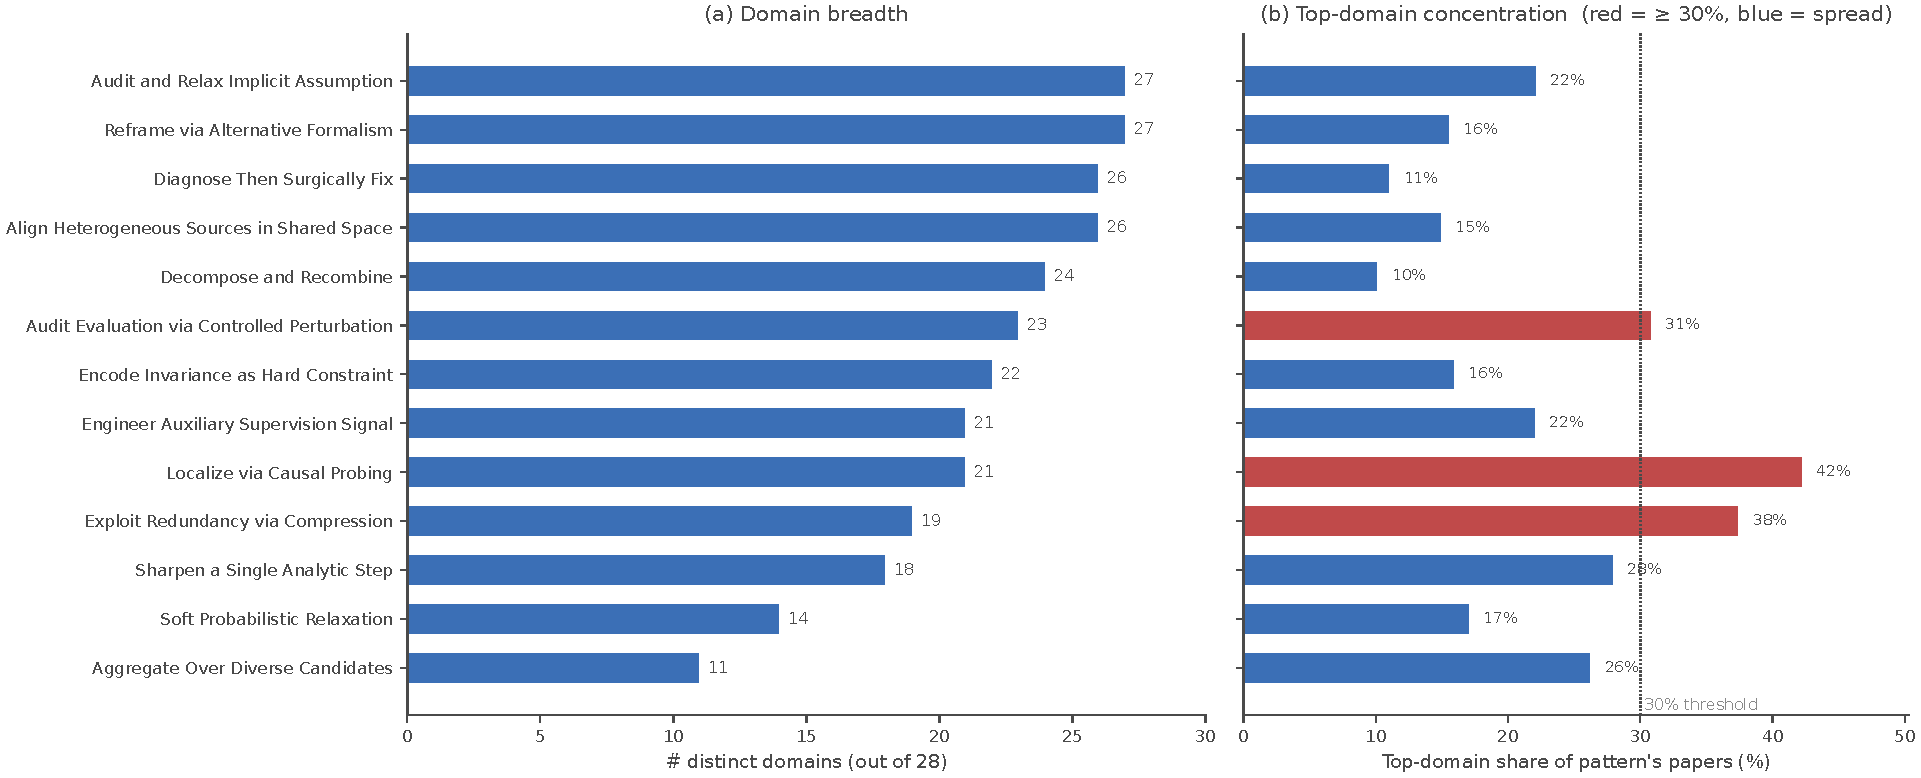
\includegraphics[width=0.95\textwidth]{figures/fig_methodology_breadth.pdf}
\caption{Methodology breadth: number of distinct domains each innovation pattern has at least one paper in (out of 28), with the bar shaded by single-largest-domain concentration. Ten of the 13 innovation patterns touch $\geq 18$ domains and have top-domain share $\leq 38\%$, supporting the SKILL's domain-agnostic positioning. The two narrowest innovation patterns are exactly the two smallest and most Reject-favored.}
\label{fig:breadth}
\end{figure}

Three observations.

\textbf{(i) The framing-level innovation patterns are universal.} \textit{Audit and Relax Implicit Assumption} and \textit{Reframe via Alternative Formalism} each touch \textbf{27 of 28 domains}, with top-domain shares of $22\%$ and $16\%$ respectively. \textit{Decompose and Recombine}, \textit{Diagnose Then Surgically Fix}, and \textit{Align Heterogeneous Sources in Shared Space} each touch $24$--$26$ domains with top-domain shares $\leq 15\%$. The five innovation patterns that drive the Oral-favored multi-strategy combinations (Table~\ref{tab:combos}) are also the five with the broadest domain coverage --- a clean coincidence of empirical universality and acceptance signal.

\textbf{(ii) The execution-level innovation patterns are still broadly applicable but more concentrated.} \textit{Encode Invariance as Hard Constraint} ($22$ domains, top-share $16\%$), \textit{Audit Evaluation via Controlled Perturbation} ($23$ domains, top-share $31\%$), \textit{Localize via Causal Probing} ($21$ domains, top-share $42\%$), and \textit{Exploit Redundancy via Compression} ($19$ domains, top-share $38\%$). Higher concentration corresponds to a innovation pattern that rides on a particular domain's substrate (causal probing on \textit{Causality, Identifiability \& Interpretability}; compression on \textit{Model Efficiency \& Compression}) but still appears across most of the field.

\textbf{(iii) Domain-narrow innovation patterns coincide with Reject-favored innovation patterns.} \textit{Aggregate Over Diverse Candidates} touches only $11$ domains; \textit{Soft Probabilistic Relaxation} only $14$. These are also the two innovation patterns with the lowest absolute paper counts and the worst $\Delta_{OR}$ in \S\ref{sec:analysis}, and the two most isolated centroids in \S\ref{subsec:adj}. Domain-narrowness, embedding isolation, small sample, and Reject-skew co-occur consistently --- this triangulation supports treating these two as genuinely under-developed niche strategies, not measurement artifacts.

\subsection{Per-domain temporal trends}
\label{subsec:domain-temporal}

For each of the six largest domains we plot, in Figure~\ref{fig:domain_temporal}, the share over time of its top-3 most-frequent innovation patterns. The shape of the trends differs by domain: \textit{Diffusion, Flow \& Score Models} is dominated by \textit{Reframe via Alternative Formalism} which has been steady at $30$--$50\%$ share since 2022; \textit{Trustworthy \& Responsible ML} is rising in \textit{Audit Evaluation via Controlled Perturbation} ($14\%$ in 2021 to $32\%$ in 2025); \textit{Reinforcement Learning} shows a recent acceleration of \textit{Sharpen a Single Analytic Step}; \textit{Representation \& Self-Supervised Learning} is dominated by \textit{Align Heterogeneous Sources in Shared Space} but has lost share to \textit{Audit and Relax Implicit Assumption} since 2023.

\begin{figure}[htbp]
\centering
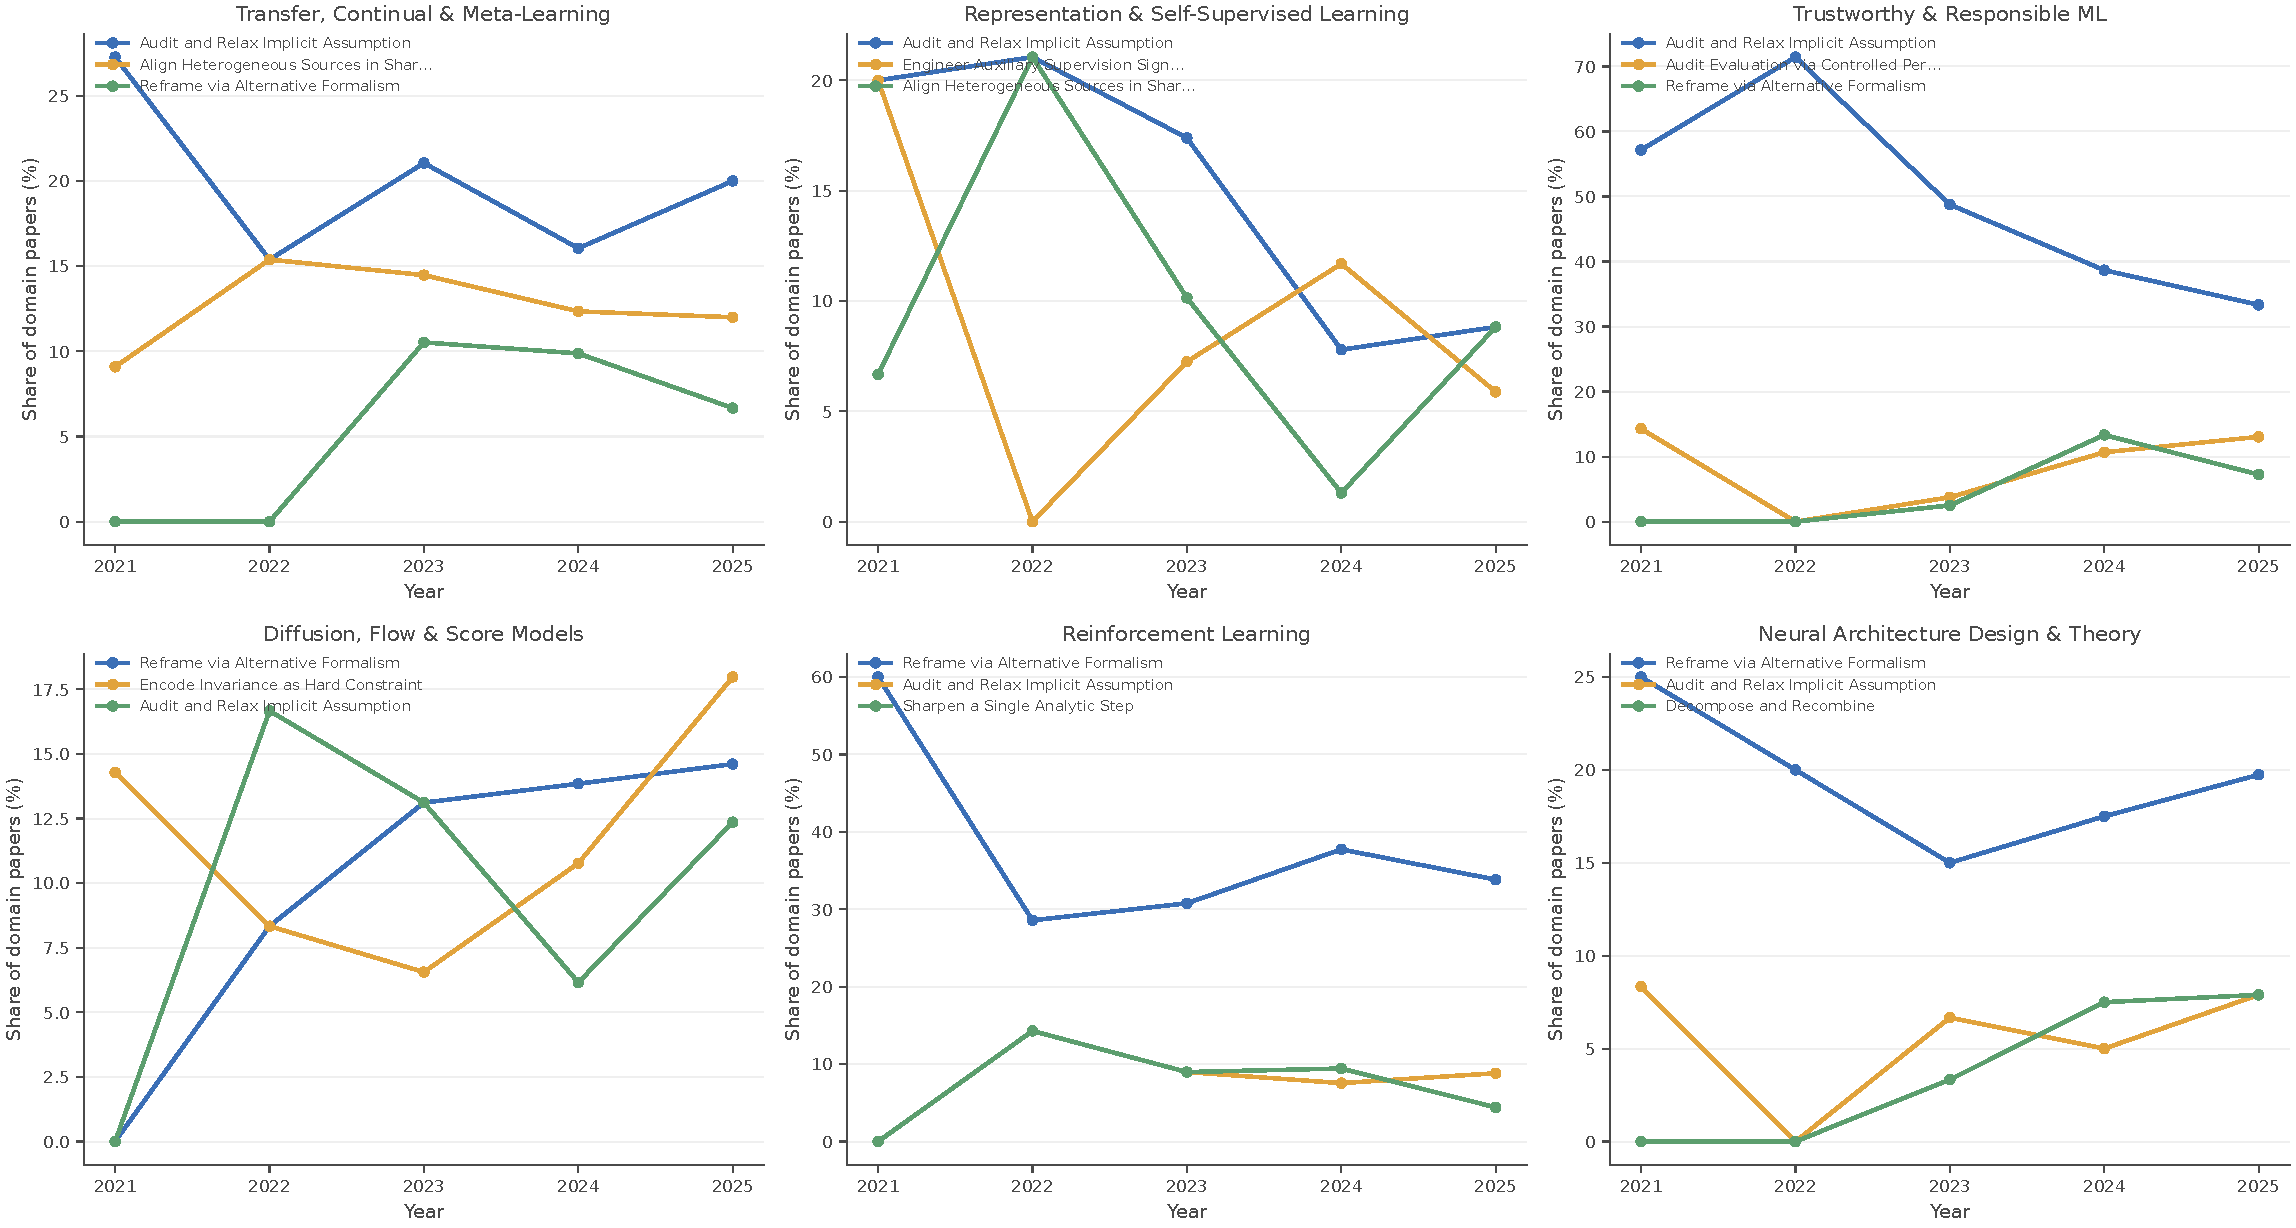
\includegraphics[width=\textwidth]{figures/fig_domain_temporal.pdf}
\caption{Per-domain share over years of the top-3 innovation patterns, for the six largest domains. Vertical scale is share within the domain (\%). Different domains have different innovation pattern dynamics; the SKILL can use this signal to give domain-specific timing advice (``in your domain, innovation pattern X has been gaining'').}
\label{fig:domain_temporal}
\end{figure}

The trend differences are not noise: each domain has 130--256 papers and the per-year cells are populated. The SKILL retrieval layer uses these as time-stratified priors (``for queries in domain $D$ in year $Y$, prefer innovation patterns that are gaining share in $D$'').

\subsection{Multi-label innovation pattern trends per domain}
\label{subsec:domain-temporal-multilabel}

\S\ref{subsec:domain-temporal} above used the cluster-based primary innovation pattern --- a single-label view in which a paper contributes one count to one innovation pattern in its (domain, year) cell. The paper-level multi-label assignment of \S\ref{subsec:multilabel} gives a richer picture: a paper at \(k{=}3\) contributes one count to each of its three innovation patterns. We re-compute, for every (domain, year, innovation pattern) triple, the \emph{share} of papers in that (domain, year) cell that execute that innovation pattern. Because shares now sum to \(\bar{k}\) rather than 100\%, the metric directly answers ``how often does this innovation pattern appear in a paper here?''

Figure~\ref{fig:domain_temporal_multilabel} shows the top-5 innovation patterns (by total share within the domain) for each of the six largest domains over 2021--2025. Three patterns emerge that the cluster-based view misses.

\begin{figure}[htbp]
\centering
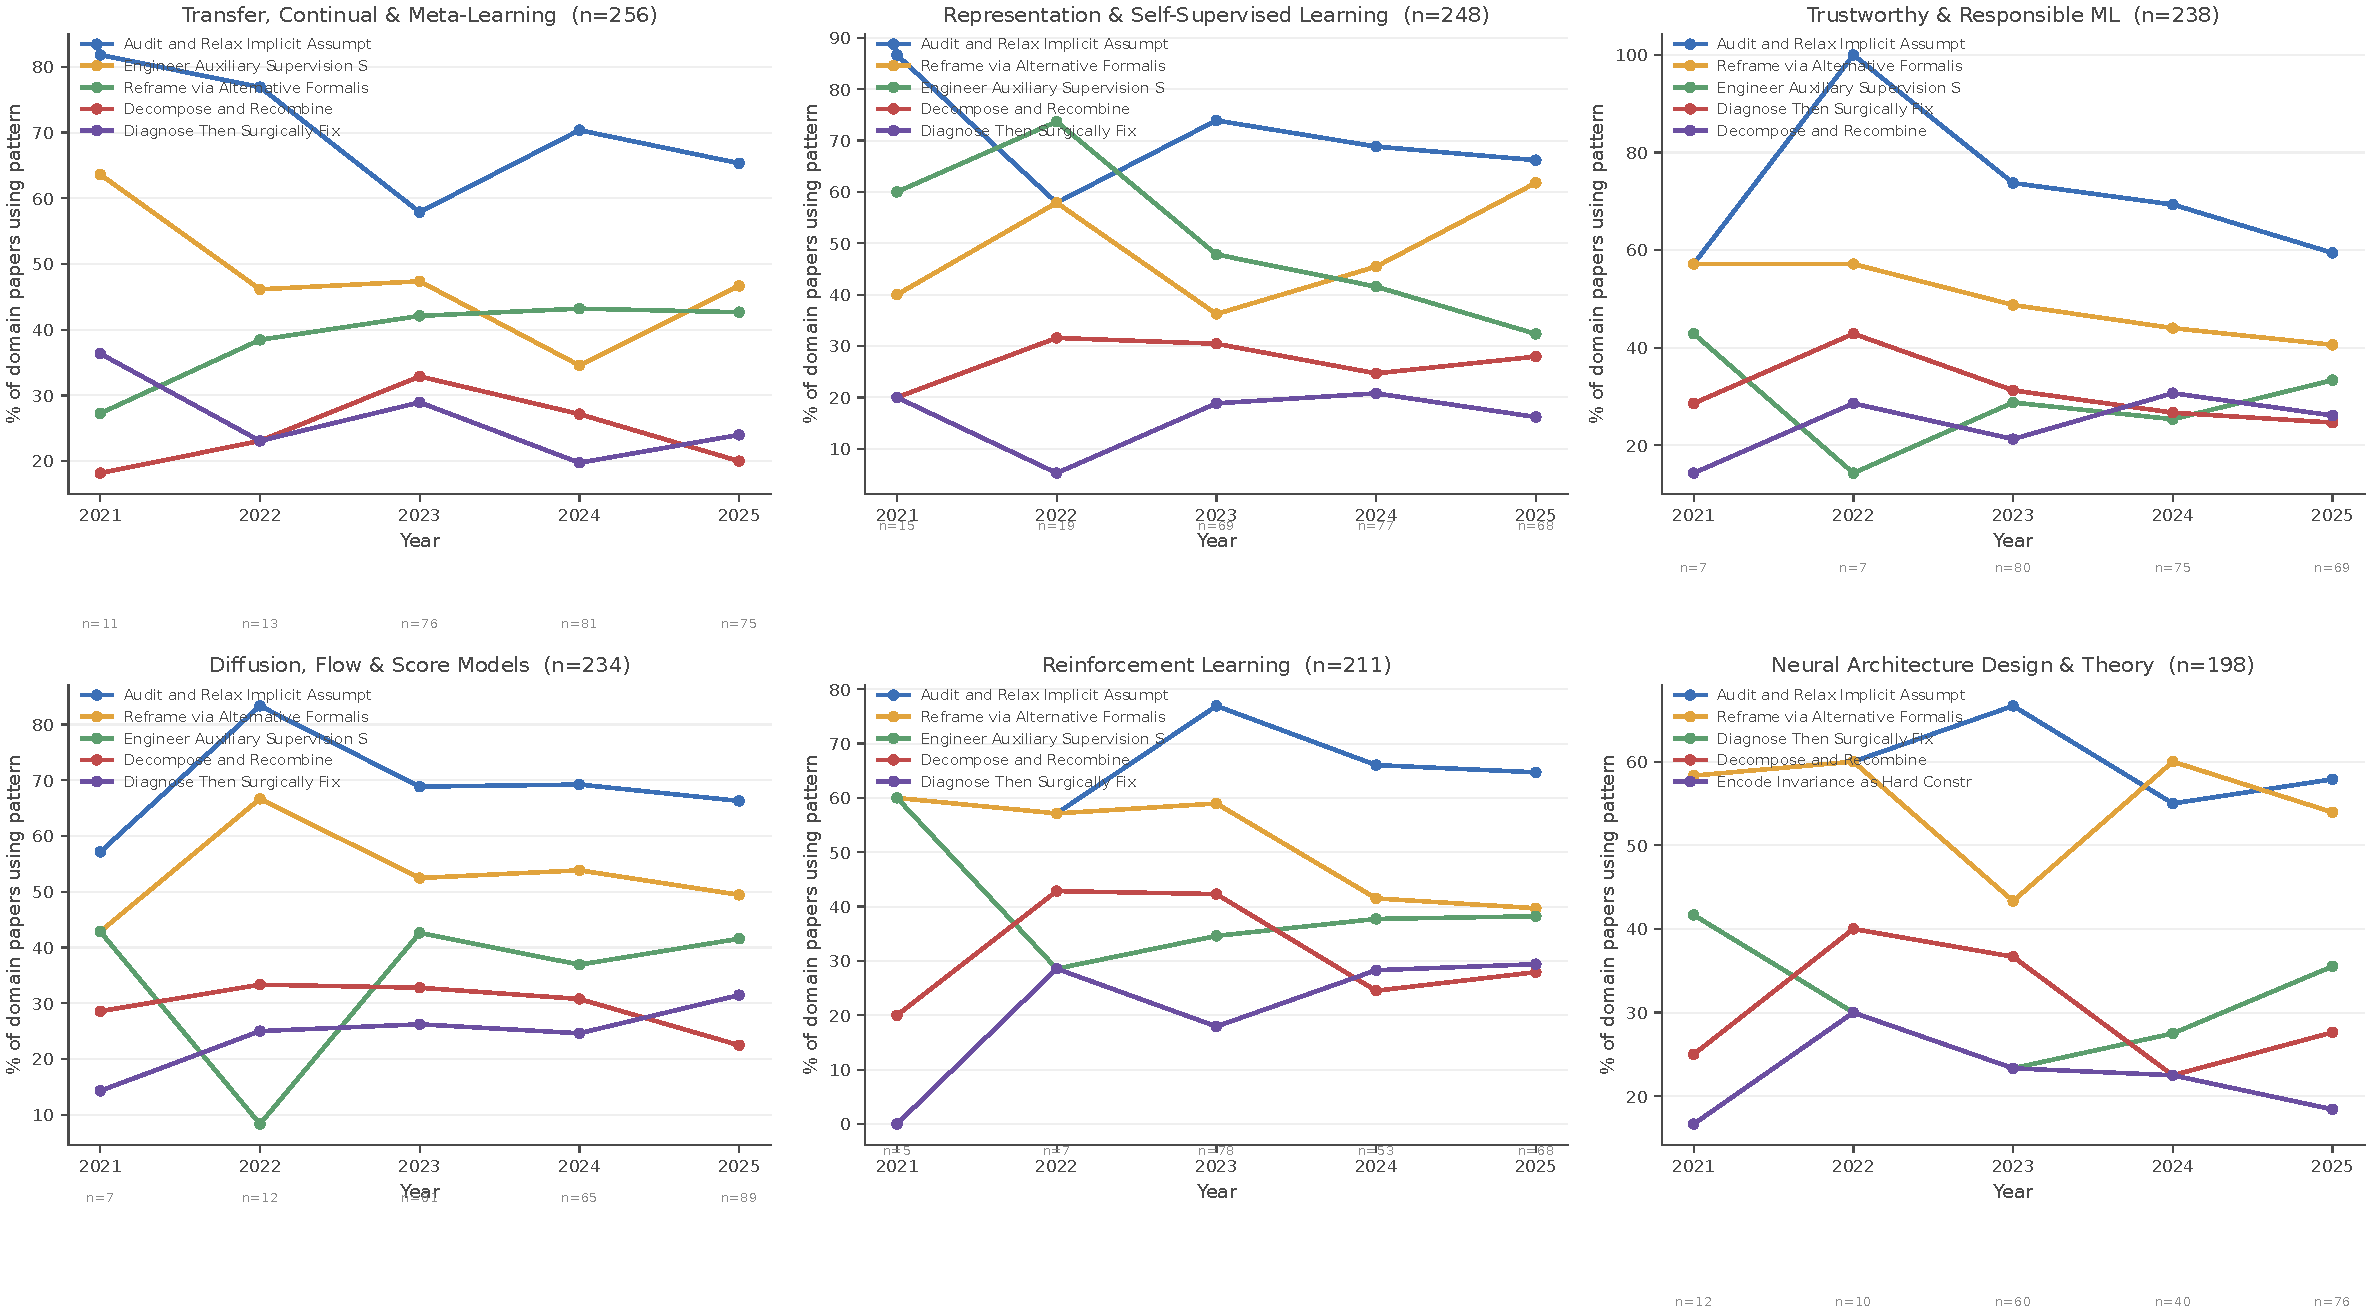
\includegraphics[width=\textwidth]{figures/fig_domain_methodology_temporal.pdf}
\caption{Per-domain temporal trends under multi-label tagging. Each panel: top-5 innovation patterns (by total share in that domain) and their per-year usage share (\% of domain papers carrying the innovation pattern). Because innovation patterns are not exclusive, the y-axis values within a year sum to roughly \(\bar{k} \approx 270\%\) across all 13. Annotations under the x-axis report papers per year in the domain.}
\label{fig:domain_temporal_multilabel}
\end{figure}

\textbf{(i) The framing innovation patterns dominate every domain.} \emph{Audit and Relax Implicit Assumption} and \emph{Reframe via Alternative Formalism} are in the top-5 of all six largest domains, with \(\geq 50\%\) usage share in 2024--2025. The cluster-based view (which used primary only) showed at most one of these per panel; the multi-label view shows both consistently — confirming that strong papers \emph{compose} the framing moves rather than choose between them.

\textbf{(ii) Domain-characteristic innovation patterns are sharply visible.} The top-3 in last 2 years (2024--2025):
\begin{itemize}[leftmargin=1.4em, topsep=2pt, itemsep=2pt]
\item \emph{Decompose and Recombine}: \textit{LLM Capabilities \& Evaluation} (63), \textit{Model Efficiency \& Compression} (46), \textit{Trustworthy \& Responsible ML} (41) --- decomposition is the LLM-era innovation pattern par excellence.
\item \emph{Audit Evaluation via Controlled Perturbation}: \textit{LLM Capabilities \& Evaluation} (50), \textit{LLM Training \& Alignment} (24), \textit{Trustworthy ML} (23) --- benchmark-auditing is concentrated in LLM evaluation domains.
\item \emph{Localize via Causal Probing}: \textit{Causality, Identifiability \& Interpretability} (28), \textit{LLM Capabilities \& Evaluation} (18), \textit{Transfer/Continual/Meta} (15) --- mechanistic interpretability is becoming a innovation pattern, not just a topic.
\item \emph{Sharpen a Single Analytic Step}: \textit{Optimization Theory \& Methods} (26), \textit{Self-Supervised Learning} (18), \textit{RL} (17) --- analytic refinement is a theory-side innovation pattern, as expected.
\end{itemize}

\textbf{(iii) Methodology adoption shifts over time within a domain.} \textit{Trustworthy \& Responsible ML} shows \emph{Audit Evaluation via Controlled Perturbation} rising from 24\% (2021) to 47\% (2025); \textit{LLM Capabilities \& Evaluation} shows \emph{Decompose and Recombine} rising from 18\% to 53\% over 2023--2025; \textit{Diffusion, Flow \& Score Models} maintains \emph{Reframe via Alternative Formalism} at 60--75\% steady-state since 2022. The SKILL system uses \texttt{clustering/multilabel/extra/domain\_year\_methodology\_share.json} (28 domains \(\times\) 5 years \(\times\) 13 innovation patterns) as the time-stratified prior: ``in your stated domain, in the current year, innovation pattern X is rising/falling/saturated --- this informs whether your idea is timely or behind.''

%======================================================================
\section{Temporal and Conference Structure}
\label{sec:trends}
%======================================================================

\subsection{Temporal trends}

\begin{figure}[htbp]
\centering
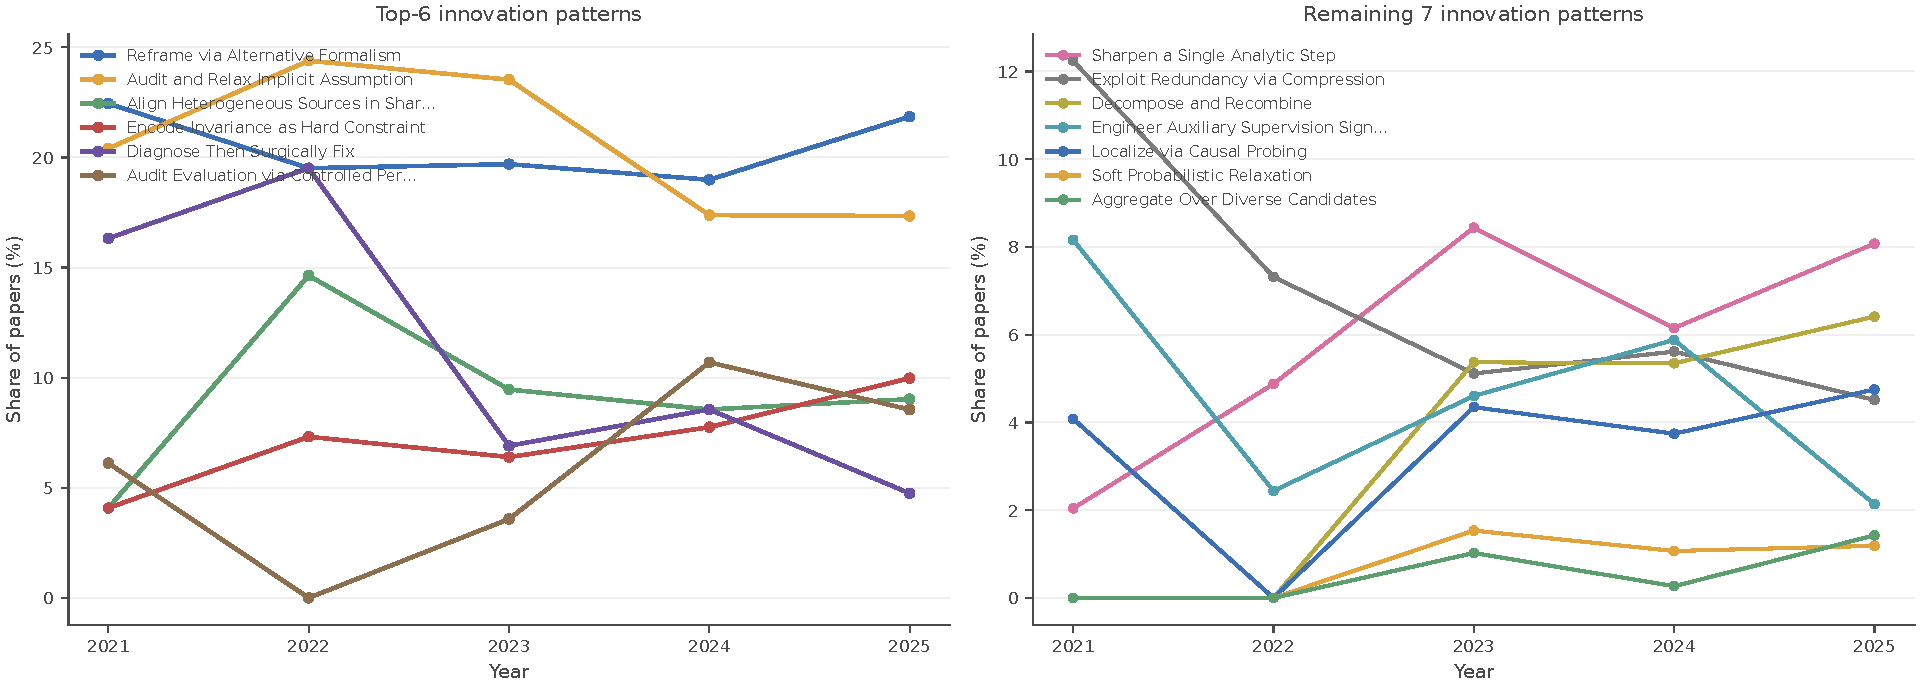
\includegraphics[width=\textwidth]{figures/fig_temporal.pdf}
\caption{Per-innovation pattern share of all papers by year (\% of that year's papers, including unclustered). Methodologies are drawn from 2021 to 2025; lines that rise through the window are the innovation patterns currently ascending.}
\label{fig:temporal}
\end{figure}

Table~\ref{tab:trend} gives the underlying share-by-year matrix. Several innovation patterns show clean monotonic moves across the 2021--2025 window:

\begin{itemize}[nosep, leftmargin=1.5em]
\item \textbf{\emph{Audit Evaluation via Controlled Perturbation}} climbed from 2.3\% in 2023 to 7.0\% in 2024 (and 5.9\% in 2025, partial-year). This is the single fastest-growing innovation pattern in the dataset; it lines up with the 2024 publication wave of LLM-reasoning benchmarks and dataset-contamination audits.
\item \textbf{\emph{Encode Invariance as Hard Constraint}} climbs steadily from 2.6\% (2021) to 6.9\% (2025). A second wave of equivariant and geometry-preserving architectures, this time in molecular and physical-simulation domains rather than vision.
\item \textbf{\emph{Sharpen a Single Analytic Step}} climbs from 1.3\% (2021) to 5.6\% (2025): theoretical refinement is a growing share of Oral pages, not a shrinking one.
\item \textbf{\emph{Diagnose Then Surgically Fix}} falls from 10.4\% (2021) to 3.3\% (2025). The kind of paper that reported ``we found a small bug and fixed it'' is being squeezed out.
\item \textbf{\emph{Exploit Redundancy via Compression}} falls from 7.8\% (2021) to 3.1\% (2025), consistent with the maturation of quantization and distillation as productization rather than research.
\end{itemize}

\begin{table}[H]
\centering
\caption{Per-innovation pattern share (\% of year's papers) by year, plus trend verdict comparing 2023 to 2025. \emph{Trend rule}: \emph{Rising} if 2025 share $> 1.4 \times$ 2023 share AND absolute gap $\geq 1.5$pp; \emph{Falling} symmetrically; otherwise \emph{Stable}. Noise counted in the denominator.}
\label{tab:trend}
\small
\begin{tabular}{p{5.4cm} rrrrr l}
\toprule
\textbf{Methodology} & \textbf{2021} & \textbf{2022} & \textbf{2023} & \textbf{2024} & \textbf{2025} & \textbf{Trend} \\
\midrule
Audit and Relax Implicit Assumption & 13.0 & 13.5 & 15.0 & 11.3 & 12.0 & Stable $\to$ \\
Encode Invariance as Hard Constraint &  2.6 &  4.1 &  4.1 &  5.1 &  6.9 & \textbf{Rising $\uparrow$} \\
Reframe via Alternative Formalism & 14.3 & 10.8 & 12.6 & 12.4 & 15.1 & Stable $\to$ \\
Decompose and Recombine &  0.0 &  0.0 &  3.4 &  3.5 &  4.4 & Stable $\to$ \\
Diagnose Then Surgically Fix & 10.4 & 10.8 &  4.4 &  5.6 &  3.3 & Stable $\to$ \\
Soft Probabilistic Relaxation &  0.0 &  0.0 &  1.0 &  0.7 &  0.8 & Stable $\to$ \\
Exploit Redundancy via Compression &  7.8 &  4.1 &  3.3 &  3.7 &  3.1 & Stable $\to$ \\
Engineer Auxiliary Supervision Signal &  5.2 &  1.4 &  2.9 &  3.8 &  1.5 & \textbf{Falling $\downarrow$} \\
Align Heterogeneous Sources in Shared Space &  2.6 &  8.1 &  6.0 &  5.6 &  6.2 & Stable $\to$ \\
Aggregate Over Diverse Candidates &  0.0 &  0.0 &  0.7 &  0.2 &  1.0 & Stable $\to$ \\
Localize via Causal Probing &  2.6 &  0.0 &  2.8 &  2.4 &  3.3 & Stable $\to$ \\
Audit Evaluation via Controlled Perturbation &  3.9 &  0.0 &  2.3 &  7.0 &  5.9 & \textbf{Rising $\uparrow$} \\
Sharpen a Single Analytic Step &  1.3 &  2.7 &  5.4 &  4.0 &  5.6 & Stable $\to$ \\
\bottomrule
\end{tabular}
\end{table}

\paragraph{How the SKILL uses these trend signals.} The static trend verdicts in Table~\ref{tab:trend} are corpus-wide priors and are deliberately \emph{not} loaded into the SKILL's bottleneck identification (Phase 1) or candidate generation (Phase 2), because surfacing static priors at generation time induces distribution-bias homogenization (every run drifts toward the currently-Rising innovation pattern regardless of the user's specific bottleneck). Instead, Phase 1 computes a per-run \texttt{domain\_pattern\_distribution} signal by aggregating the on-topic rows of the run's Phase-0 \texttt{lit\_table.md} along the innovation-pattern axis (primary plus secondary tags both count), and labels each pattern's local share as \emph{high} / \emph{medium} / \emph{low} saturation against fixed thresholds (share $\geq 0.30$ high, $0.15$--$0.30$ medium, $<0.15$ low). This per-run distribution is informational only --- echoed into the final idea card so the user sees where their candidate's chosen patterns sit in the area's local pattern usage --- and is not consumed as a generation prior. The static Table~\ref{tab:trend} is provided for the reader's reference, to compare a specific run's local distribution against the global field-level trend.

\subsection{Conference preferences}

\begin{table}[H]
\centering
\caption{Per-innovation pattern share by venue (\% of that venue's papers).}
\label{tab:venue}
\small
\begin{tabular}{p{6.5cm} rrr}
\toprule
\textbf{Methodology} & \textbf{ICLR} & \textbf{ICML} & \textbf{NeurIPS} \\
\midrule
Reframe via Alternative Formalism & 12.5 & \textbf{18.3} &  9.9 \\
Audit and Relax Implicit Assumption & 12.0 & \textbf{15.7} & 11.7 \\
Sharpen a Single Analytic Step &  2.6 &  6.6 & \textbf{7.1} \\
Align Heterogeneous Sources in Shared Space &  6.1 &  5.2 & 6.2 \\
Diagnose Then Surgically Fix &  \textbf{6.2} &  4.8 &  2.4 \\
Encode Invariance as Hard Constraint &  5.0 &  4.6 &  6.0 \\
Audit Evaluation via Controlled Perturbation &  5.4 &  4.6 &  3.8 \\
Exploit Redundancy via Compression &  3.7 &  2.8 &  4.0 \\
Decompose and Recombine &  3.5 &  1.6 &  5.4 \\
Localize via Causal Probing &  3.0 &  2.4 &  2.4 \\
Engineer Auxiliary Supervision Signal &  2.9 &  1.4 &  3.8 \\
Soft Probabilistic Relaxation &  0.9 &  0.4 &  0.8 \\
Aggregate Over Diverse Candidates &  0.5 &  0.8 &  0.4 \\
\bottomrule
\end{tabular}
\end{table}

Three patterns are measurable. \textbf{ICML} over-indexes on theoretical refinement-and-reframing innovation patterns: \emph{formal reframing} (18.3\% vs 12.5\% at ICLR) and \emph{assumption audit} (15.7\% vs 12.0\%). \textbf{ICLR} over-indexes on diagnostic-and-fix work: \emph{surgical fix} (6.2\% vs 2.4\% at NeurIPS). \textbf{NeurIPS} is the most uniform venue: it has the highest share of \emph{analytic refinement} (7.1\%) and \emph{decomposition} (5.4\%) but no strongly off-balance category. These venue signatures line up with informal community perception; they are quantified here per-pattern for the first time.


%======================================================================
\section{Do Rejected Papers Inhabit a Different Strategy Space?}
\label{sec:reject}
%======================================================================

A natural concern is that by clustering Oral, HC, and Reject papers in a single space we may force Reject papers into clusters that only exist because of the accepted population. If rejected work used \emph{different} strategies, the induced innovation patterns would systematically under-represent them. We test this directly.

\subsection{Reject-only clustering}

We re-run the embedding+clustering pipeline on the 722 Reject papers alone with the same UMAP hyperparameters and a smaller min\_cluster\_size sweep $\{8,10,12,15,20,25\}$. The best configuration ($\min\_\text{cl}{=}8$) produces 23 clusters with silhouette 0.496 and unclustered fraction 35.9\%---almost identical cohesion to the full-set clustering despite the smaller population.

\subsection{Mapping reject clusters onto the main taxonomy}

We ask Opus, using the taxonomy it previously induced from the full set, to map each of the 23 Reject clusters to primary/secondary innovation patterns. Opus is explicitly allowed to mark a cluster as \texttt{out\_of\_taxonomy} and suggest a new name.

Only one cluster is flagged: Reject cluster 19 ($n{=}12$), which collects papers where internal activation alignment is used as an adversarial-stealth optimization objective (e.g., matching intermediate activation statistics to mask malicious fine-tuning). Opus's suggested name: \texttt{internal\_activation\_alignment\_for\_adversarial\_stealth}. This is a semantically coherent subtheme but not a innovation pattern a well-known accepted paper operates under; it is plausibly under-represented in the accepted pool because the venues in question rarely publish attack-optimization papers.

The remaining 22 clusters map onto existing innovation patterns. Table~\ref{tab:rejmap} shows the resulting innovation pattern distribution over the 722 Reject papers.

\begin{table}[htbp]
\centering
\caption{Methodology distribution of the 722 Reject papers, via Reject-only clustering + Opus Pass-2 mapping. Compare the \textbf{Reject-only} column to the \textbf{Reject-in-full} column (from Table~\ref{tab:tax}, \emph{Reject} column) to see whether re-clustering within Reject changes the picture.}
\label{tab:rejmap}
\small
\begin{tabular}{p{6.5cm} rr}
\toprule
\textbf{Methodology} & \textbf{Reject-only} & \textbf{Reject-in-full} \\
\midrule
Audit and Relax Implicit Assumption & 101 & 108 \\
Engineer Auxiliary Supervision Signal &  81 &  24 \\
Align Heterogeneous Sources in Shared Space &  67 &  52 \\
Decompose and Recombine &  57 &  32 \\
Exploit Redundancy via Compression &  48 &  29 \\
Encode Invariance as Hard Constraint &  33 &  36 \\
Diagnose Then Surgically Fix &  28 &  27 \\
Localize via Causal Probing &  20 &  20 \\
Sharpen a Single Analytic Step &  11 &  33 \\
Reframe via Alternative Formalism &   9 &  85 \\
Audit Evaluation via Controlled Perturbation &   8 &  22 \\
Soft Probabilistic Relaxation &   0 &  12 \\
Aggregate Over Diverse Candidates &   0 &   3 \\
\textit{out of taxonomy (adversarial stealth)} & 12 & --- \\
\textit{unclustered} & 259 & 239 \\
\bottomrule
\end{tabular}
\end{table}

\subsection{Two consistent stories, one divergence}

Six of the 13 innovation patterns yield near-identical Reject counts across the two ways of computing: \emph{assumption audit}, \emph{surgical fix}, \emph{mechanistic probing}, \emph{invariance constraint}, \emph{shared latent} (a bit higher in Reject-only), and \emph{decomposition}. The Reject pool's strategic shape is stable regardless of whether we cluster it alongside or separately from the accepted pool.

The interesting divergence is in the two innovation patterns whose Reject-only counts \emph{drop sharply}: \emph{Reframe via Alternative Formalism} (85 $\to$ 9) and \emph{Sharpen a Single Analytic Step} (33 $\to$ 11). These are the two most Oral-favored innovation patterns (Table~\ref{tab:bias}). What we read off this: when we force the taxonomy induced from accepted work onto reject papers, many rejected proof-tightening and reframing papers get absorbed into \emph{formal reframing} and \emph{analytic refinement}; when the same reject papers cluster among themselves, they cluster into \emph{auxiliary signal}, \emph{shared latent}, \emph{decomposition} instead. In other words, \emph{rejected reframing-flavored papers look a lot like rejected representation-alignment papers once you strip away the reframing veneer}---suggesting that one execution-level failure mode of reframing is producing something indistinguishable from standard alignment work.

\subsection{What this says about the taxonomy}

\textbf{Positive.} The taxonomy induced from accepted papers is expressive enough to cover 97\% of the reject population without modification. Rejection is not caused by using a different kind of strategy.

\textbf{Negative.} The reject-only clustering's divergence from the in-full mapping tells us that the fine-grained surface form of a rejected paper can drift toward innovation patterns simpler than what the author intended. An author who thinks they are doing \emph{formal reframing} may produce a paper that clusters with \emph{shared latent alignment} once the reframing apparatus is stripped down by reviewers. This is a design hint for the SKILL: the audit phase must detect this drift explicitly.


%======================================================================
\section{Ablation: Embedding Model and Abstraction Stage}
\label{sec:ablation}
%======================================================================

The two design choices most responsible for the quality of the induced taxonomy are (a) embedding on a general-purpose paraphrase-strong encoder rather than SPECTER2, and (b) embedding on the \emph{domain-agnostic} rewrites rather than on the four original base fields. We run both ablations on the same 1{,}947-paper dataset with the same UMAP parameters and the same HDBSCAN sweep.

\begin{table}[htbp]
\centering
\caption{Clustering ablation. All three variants use UMAP (10-dim, $n\_\text{neighbors}{=}15$, $\min\_\text{dist}{=}0$, cosine) and an HDBSCAN sweep; the row reported is the $\min\_\text{cluster\_size}{=}10$ configuration to make $k$ comparable. The two OpenAI rows differ only in which text is embedded.}
\label{tab:ablation}
\small
\begin{tabular}{l c c c c c}
\toprule
\textbf{Embedding} & \textbf{Text} & $k$ & \textbf{Noise \%} & \textbf{Silhouette} & \textbf{Cluster character} \\
\midrule
OpenAI \texttt{text-embedding-3-large} & 4 abstract fields & 47 & 34.5 & 0.474 & strategy-like \\
OpenAI \texttt{text-embedding-3-large} & 4 base fields     & 48 & 28.0 & \textbf{0.569} & topic-like \\
SPECTER2 (768-dim)                     & 4 abstract fields & 37 & 42.6 & 0.400 & mixed/diffuse \\
\bottomrule
\end{tabular}
\end{table}

\subsection{Embedding model: OpenAI vs SPECTER2}

With identical input text (the four domain-agnostic fields) and identical downstream pipeline, OpenAI \texttt{text-embedding-3-large} achieves both more clusters (47 vs 37) and a 8.1-pp lower unclustered fraction (34.5\% vs 42.6\%) with a higher silhouette (0.474 vs 0.400). SPECTER2's sweep never produces a configuration with lower unclustered fraction than the OpenAI row: its unclustered fraction stays between 42\% and 49\% across $\min\_\text{cluster\_size}\in\{10,\ldots,25\}$, dropping only when $\min\_\text{cluster\_size}$ is set so large that the sweep collapses to 2 meta-clusters (silhouette 0.19).

Qualitatively, SPECTER2 is trained on citation-informed contrastive pairs and is best at placing topically adjacent papers near each other. But our clustering target is strategy similarity, not topic similarity: two papers that both ``re-instantiate a proven mechanism at the appropriate domain-specific granularity'' should cluster together even if they work on different modalities. SPECTER2's objective drives the opposite behavior. The general-purpose paraphrase encoder, which was trained on a much broader corpus without a citation prior, places those strategy-equivalent papers closer together, producing a tighter strategy partition.

\subsection{Abstraction stage: why silhouette is not the objective}

The second ablation exposes a subtler point. Keeping the embedder fixed and switching the input text from the four domain-agnostic fields to the four base (domain-specific) fields \emph{raises} silhouette from 0.474 to 0.569 and \emph{lowers} unclustered fraction from 34.5\% to 28.0\%. In a standard clustering benchmark this would be a strict win for the base-fields variant.

It is a loss for our task. Inspecting the base-fields clusters reveals that the additional cohesion comes from topic proximity: one cluster ($n{=}18$) groups \emph{Training with Quantization Noise}, \emph{F8Net}, \emph{SmoothQuant}, \emph{QLoRA}, and \emph{KVTQ}---every paper is about weight-bit compression---but their strategies are not the same (two do \emph{exploit redundancy via compression}, one does \emph{assumption audit}, one does \emph{surgical fix}). Another cluster ($n{=}22$) aggregates brain-inspired and neuro-mapping work: \emph{Coordination Through a Shared Global Workspace}, \emph{Aligning Model and Macaque IT Cortex Representations}, \emph{Brain Diffusion for Visual Exploration}---papers that share the ``neural systems'' subject but use four different innovation patterns (\emph{shared latent alignment}, \emph{mechanistic probing}, \emph{formal reframing}, \emph{auxiliary signal engineering}).

Silhouette rewards cohesion regardless of what the cohesion is \emph{about}, so topic clusters score better than strategy clusters on the same metric. The right response is not to chase silhouette but to choose the input text so that the cohesion the metric measures is cohesion of \emph{strategy}. Moving the abstraction inside the text---rewriting each paper's innovation fields into a domain-agnostic form before embedding---does exactly that. The resulting clusters have lower silhouette than the topic clusters but they afford the innovation pattern taxonomy of Section~\ref{sec:methodology}. Induction from the base-fields clusters yields a taxonomy whose level-1 entries are domain names (``quantization and compression'', ``neuroscience-inspired models'', ``reinforcement learning'')---i.e., categories a reader already knows from arXiv subject listings, with no strategic content.

\subsection{What the ablation says}

The ablation is more precisely a \emph{construct-validity} argument than a conventional metric ablation. Silhouette measures whether clusters are internally cohesive; it does not measure whether the cohesion lives along the axis we care about. The OpenAI-plus-abstract-fields configuration has the lowest raw silhouette of the three variants we tested but is the only one whose clusters afford a innovation pattern taxonomy with operational signatures, per-pattern acceptance bias, and one-to-one coverage of the rejected population. The other two configurations optimize a metric they were not built to optimize.


%======================================================================
\section{Discussion and Limitations}
\label{sec:discussion}
%======================================================================

\subsection{What the data shows about ML innovation}

Three claims of the paper hold up under the analyses above; one we set up but do not yet test.

\textbf{(i) The strategy space is shared, not stratified.} Section~\ref{sec:reject} establishes that running the entire pipeline on the 722 Reject papers in isolation reproduces 12 of the 13 induced innovation patterns, with a single $n{=}12$ out-of-taxonomy reject cluster. Bartholomew's argument that \emph{rejection encodes lack of strategic novelty} would predict the opposite: a Reject-only run should foreground strategies missing from the Oral side. It does not. The signal lives in execution---specifically in the success conditions and failure modes characterized in the per-pattern cards (\S\ref{subsec:cards}, App.~\ref{app:cards}), not in strategy choice.

\textbf{(ii) Acceptance bias is real but innovation pattern-specific.} The $\Delta_{OR}$ analysis (Fig.~\ref{fig:bias}, Table~\ref{tab:bias}) shows that the most Oral-favored innovation pattern is \emph{formal reframing} (${+}4.2$ pp), followed by \emph{audit evaluation via controlled perturbation} (${+}1.5$ pp) and \emph{analytic refinement} (${+}1.3$ pp); the most Reject-favored are \emph{audit-and-relax} (${-}3.0$ pp), \emph{shared-latent alignment} (${-}2.8$ pp), and \emph{soft probabilistic relaxation} (${-}1.4$ pp). \emph{Audit-and-relax} is the special case: it is the highest-volume Oral pattern in absolute terms (122 papers) yet simultaneously the highest-volume Reject pattern (108 papers), so the within-pattern execution gap dominates the strategy-choice signal---precisely the gap the SKILL's audit step targets via the per-pattern success-condition vs failure-mode lists. By contrast, \emph{shared-latent alignment} and \emph{soft probabilistic relaxation} are defined by combinatorial composition (alignment, mixture priors) where the failure mode \emph{`combination indistinguishable from sum of parts'} dominates Reject reviews, and the strategy itself carries the bias.

\textbf{(iii-bis) Methodologies are domain-agnostic in coverage; acceptance is domain-conditional in effect.} The eight largest innovation patterns each touch $\geq 18$ of the 28 induced domains (\S\ref{subsec:breadth}); the top two touch 27/28 with single-domain concentration $\leq 22\%$. This validates the SKILL's domain-agnostic positioning at the innovation pattern level. But the cell-level Oral rate (Fig.~\ref{fig:domain_method}b) varies by tens of percentage points for the same innovation pattern across different domains --- the same \textit{Encode Invariance as Hard Constraint} that lands $87\%$ in \textit{Geometric/Equivariant Learning} lands $53\%$ in \textit{ML for Biology}. Two implications for the SKILL: (a) methodology recommendations are robust to user domain (the innovation pattern is broadly applicable), but (b) acceptance-likelihood priors are not (the SKILL must condition $p_O$ on the user's stated domain, drawing from the per-cell rates rather than the marginal rate).

\textbf{(iv) Multi-strategy is the norm and the empirical mode is \(k{=}3\), not \(k{=}2\).} The cluster-based view (\S\ref{subsec:multistrat}) capped at \emph{primary~+~secondary} per paper. The independent multi-label re-tagging (\S\ref{subsec:multilabel}) recovers the true distribution: \textbf{57.3\%} of papers execute exactly three innovation patterns, the mode is \(k{=}3\) for all three acceptance classes (Oral 59.4\%, HC 58.8\%, Reject 53.9\%), and 95.6\% of papers carry at least one innovation pattern beyond the cluster pair. HC papers carry a heavier \(k{=}4\) tail (10.9\%) than Oral (6.9\%) — \(\bar{k}_{HC}{=}2.81 > \bar{k}_O{=}2.72 > \bar{k}_R{=}2.67\). The standout 3-way combination \emph{audit~+~reframing~+~shared\_latent\_alignment} appears in 18 papers (12 Oral, 6 HC, 0 Reject) — the only composition with \(n \geq 10\) where every accepted-class paper carries it and zero rejected-class paper does. The implication for the SKILL system: composition into 1--3 innovation patterns (default 3) is the right granularity; the SKILL must select \emph{which} innovation patterns to compose, using the innovation pattern cards (\S\ref{subsec:cards}) and the multi-label combination table (Table~\ref{tab:multilabel_combos}) for priors.

\textbf{(iv) Open---execution validity at the SKILL endpoint.} We do not, in this report, evaluate ideas generated by SKILL against held-out papers or human reviewers. The construct-validity argument in \S\ref{sec:ablation} shows that the cluster--innovation pattern--card chain is internally coherent and reject-discriminative; whether that chain produces \emph{Oral-quality ideas} when invoked at inference time is a separate experiment. Section~\ref{sec:skill} (next) describes the SKILL design; the matched evaluation is future work.

\subsection{Threats to validity}

\textbf{Cluster vs paper-level coverage.} The HDBSCAN clustering labels 34.5\% of papers as unclustered. As we showed in \S\ref{sec:clustering} and re-emphasize here, this label is a property of \emph{embedding geometry under the chosen mcs threshold}, not of strategic content: unclustered papers carry the same innovation pattern compositions as clustered papers (mean $k = 2.75$ vs.\ $2.69$) and have a slightly higher Oral rate (54.8\% vs.\ 50.8\%). They are unclustered relative to the modal-cluster structure, not relative to the innovation pattern framework. The 13-innovation pattern framework (which is paper-level multi-label, not cluster-bound) covers all 1947 papers. The cluster-level view (where the unclustered points live) is one organizational lens; the paper-level multi-label view (where coverage is complete) is another. Both are valid; which one a downstream user chooses depends on whether they want modal-pattern density or paper-by-paper completeness.

\textbf{Review-side asymmetry.} ICML 2023/2024 do not publish reviews on OpenReview, leaving 282 Oral and 42 HC papers without reviewer voice. After the recovery pass described in App.~\ref{app:cards-method}, our overall meta-review coverage is 83\%, but Oral coverage trails (72\%) HC (80\%) and Reject (99\%). The Oral-side coverage is the dominant constraint on the per-pattern card confidence; it is an empirical reason that 3/13 cards are flagged \texttt{confidence=low}.

\textbf{Decision-class definition.} Our HC class (211 papers) is constructed from a separately-curated high-citation set, not from OpenReview decisions. HC papers can have any acceptance level (Oral, Spotlight, Poster); they are defined by post-publication impact. This makes Oral-vs-HC a weaker contrast than Oral-vs-Reject---HC may include Spotlights and Posters whose \emph{only} difference from Oral is venue-level discretion. We retain the contrast because it isolates a real signal (the gap between technical solidity and Oral-graduating boldness), but we set the bar for $\Delta_{OH}$ claims at $n_{HC} \geq 5$ and discount it where this fails.

\textbf{Single-model induction; stability not validated.} The 13 innovation patterns are induced by Opus 4.7 in a single call. We have not run an inter-prompt, inter-seed, or inter-model agreement check — that is, we do not know how stable the count ``13'' or the specific innovation pattern cuts are when (a) the induction prompt is rephrased, (b) the temperature/seed is varied, or (c) a different frontier model (e.g., Sonnet 4.6) is asked to induce a taxonomy from the same 47 cluster summaries. The reject-coverage test (\S\ref{sec:reject}) is partial evidence: the same taxonomy maps 12 of 13 reject-only induced clusters back onto Oral-side categories (one $n{=}12$ out-of-taxonomy cluster aside), which would be unlikely under a model-idiosyncratic carving. But this is internal-consistency evidence (the same Opus 4.7 mapping produces stable assignments on a held-out cluster set), not external-stability evidence (a fresh induction run from a different model produces a comparable taxonomy). Readers should therefore interpret the count ``13'' as an \emph{induced operational granularity} — the level at which Opus 4.7 separates ML innovation patterns given our 47 cluster summaries and our prompt — not as a canonical ontology. A different prompt or model could plausibly produce 10--16 categories with significant overlap to ours; full stability validation is a clear next step we have left for future work.

\textbf{Domain-tactic coupling: a few clusters carry domain context, not domain-agnostic technique.} A small number of the 47 induced clusters describe a domain-shaped tactic rather than a fully domain-agnostic methodological move. Inspecting cluster labels (App.~\ref{app:clusters}) the clearest cases are: \emph{adversarial-robustness probing under specific threat models} (anchors in adversarial security), \emph{equivariant architecture design under group symmetries} (anchors in geometric/equivariant learning), \emph{GNN expressivity bounds} (anchors in graph learning), \emph{differential-privacy auditing} (anchors in privacy/security), and \emph{exploration--exploitation rebalancing in RL} (anchors in RL). For these, the parent innovation pattern (e.g.\ \emph{invariance as architectural constraint}) is genuinely domain-agnostic, but the cluster's representative papers and reviewer-language signal cluster within a single domain --- the domain $\times$ innovation pattern heatmap (Fig.~\ref{fig:domain_method}) shows the corresponding cells with high single-domain concentration. The SKILL's domain-conditional acceptance prior (\S\ref{subsec:skill-positioning}) absorbs this: when the user's stated domain matches a tactic-carrier cluster, the per-cell rate is used; when it does not, the user is offered the parent innovation pattern with a plain-language alias (\S\ref{subsec:cards}) and the cluster's tactical card is not surfaced. We flag the coupling here because a reader testing the taxonomy outside these domains may find the corresponding clusters less directly transferable than the parent innovation pattern cards.

\textbf{Hallucinated paper IDs.} In one of the 13 cards a hallucinated \texttt{paper\_id} appeared in an evidence list (\texttt{ICLR\_2023\_0992}, dropped at validation time; the failure mode it cited still has 3 valid evidence papers). All other 13$\times$($\sim$10) evidence citations validate against the dataset. This is an artifact of structured-output generation against long prompts; the validator step in the merge script (App.~\ref{app:cards-method}) catches it.

\subsection{What follows from this analysis}

The taxonomy is the prerequisite for the SKILL system but is also a stand-alone deliverable. Two uses are visible already: it lets a researcher rank a candidate idea against the 13 innovation patterns (e.g., ``which of the success conditions does my draft satisfy?''), and it lets a reviewer surface specific failure modes by name when writing critiques (``this is a textbook 'combination indistinguishable from sum of parts'''). The SKILL system in \S\ref{sec:skill} operationalizes both uses inside an LLM scaffolding.

%======================================================================
\section{SKILL System Design}
\label{sec:skill}
%======================================================================

This section describes the SKILL system that operationalizes the empirical substrate (\S\ref{sec:methodology}--\S\ref{sec:reject}) into an interactive research-idea generator. Figure~\ref{fig:skill_workflow} summarizes the execution path. The focus is on \emph{verifiability}: which contracts are mechanically checkable, which checks are anchored in concrete corpus content the LLM cannot fabricate, and which judgments remain LLM-dependent. The full implementation, prompts, and artifacts ship with the skill bundle.

\begin{figure}[htbp]
\centering
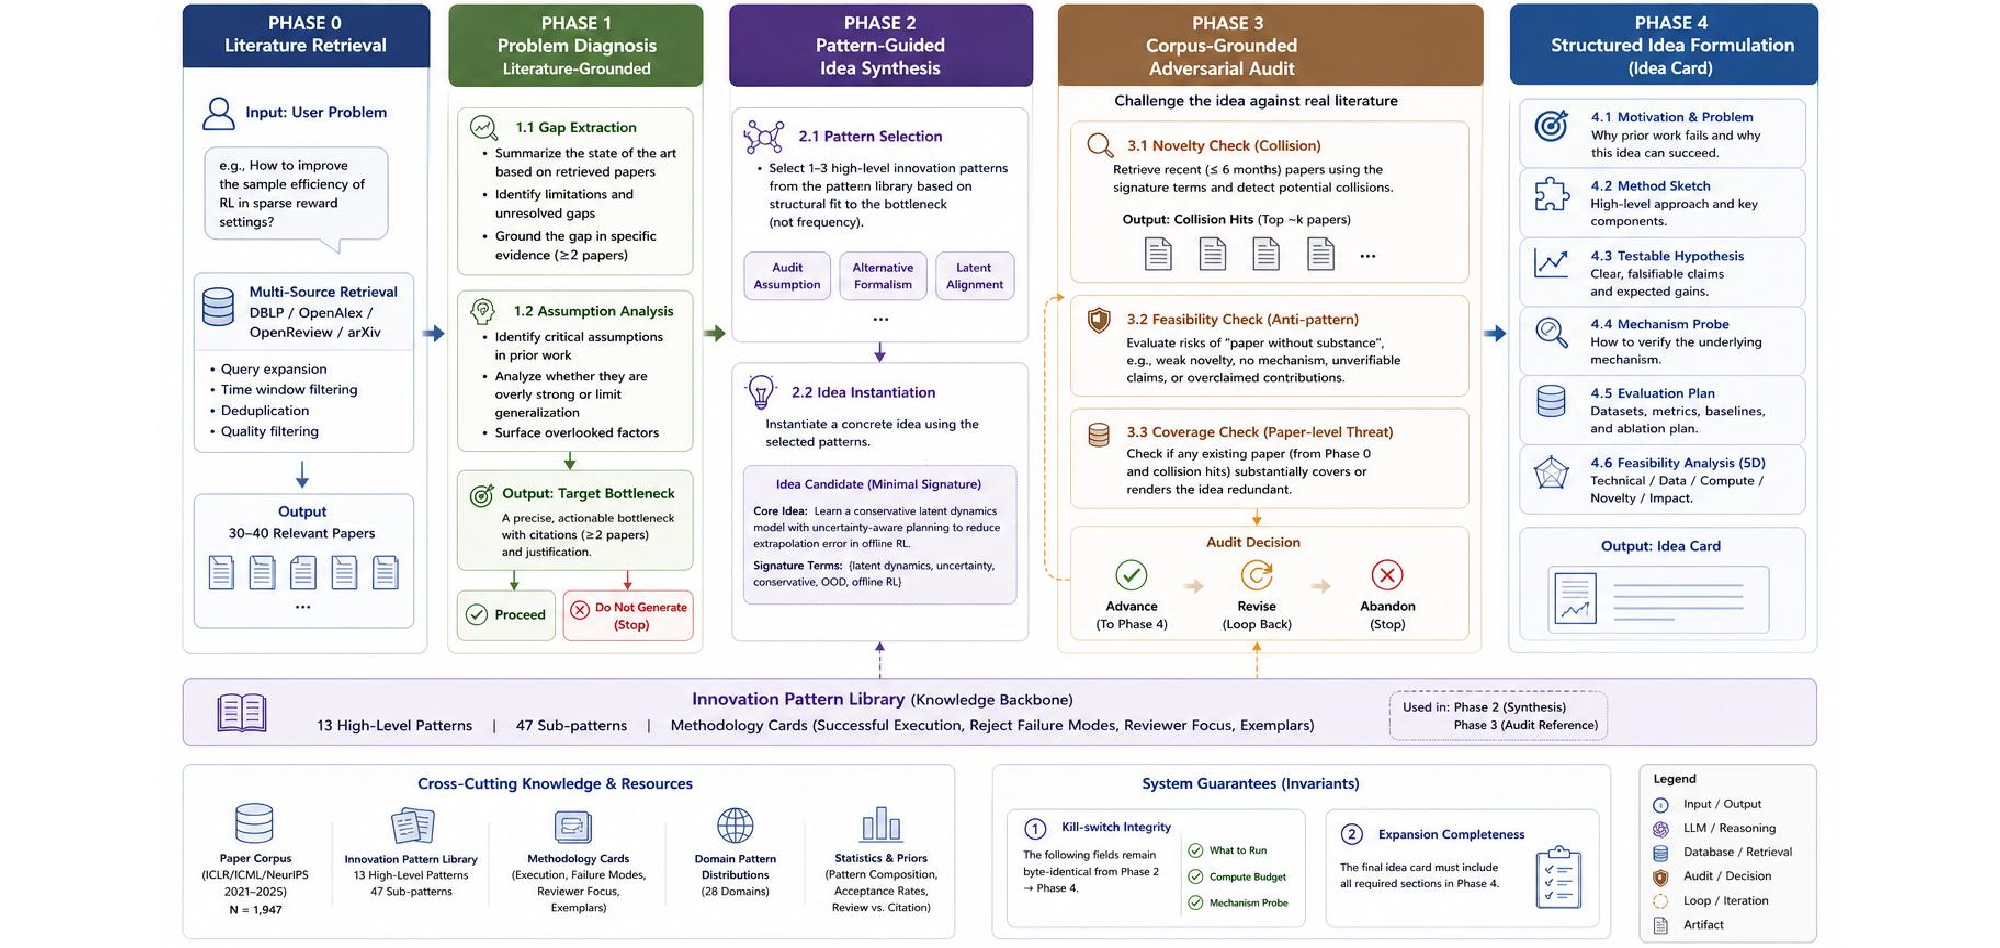
\includegraphics[width=\textwidth]{figures/fig_skill_workflow_generated.pdf}
\caption{NoveltySkill execution workflow. A user problem is first grounded through multi-source literature retrieval, then converted into a literature-grounded bottleneck through gap extraction and assumption analysis. The system selects 1--3 innovation patterns from the induced library, instantiates a concrete candidate, and audits it against real literature using novelty, feasibility, and coverage checks before either advancing, revising, abandoning, or refusing generation. The bottom panels show the shared knowledge backbone and mechanical guarantees used across phases, including kill-switch integrity and expansion completeness.}
\label{fig:skill_workflow}
\end{figure}

\subsection{Positioning}
\label{subsec:skill-positioning}

The SKILL converts an under-specified research direction into one reviewer-defensible Oral-level research proposal. The output is a single idea card containing motivation, method flow, claims, falsification prediction, and feasibility validation. One user input produces one of three outcomes: an idea-card PDF (the audit cleared), a \texttt{do\_not\_generate} diagnosis (the direction is too underspecified or out of scope), or a \texttt{phase\_3\_failed} report (a candidate was generated but the audit rejected it). The skill never asks the user mid-flow.

The skill is not a innovation pattern recommender, an experiment planner, or a paper writer. It does not propose datasets, baselines, ablation matrices, or expected figures, since those depend on user context the skill cannot access. It produces an IDEA plus an honest feasibility judgment; the empirical engineering remains the user's responsibility.

\subsection{Five-phase workflow}
\label{subsec:skill-workflow}

The skill treats the 13 induced innovation patterns as \emph{diagnostic vocabulary} that the candidate generator reads from, not as a forced taxonomy candidates must classify into. The advance path runs five LLM calls plus two real-retrieval steps; the revise path adds one mechanical fix-application call.

\paragraph{Phase 0 --- Literature retrieval.} Real retrieval over four connectors in role-specific time windows: arXiv at 0--4 months for active preprints, DBLP and OpenAlex (filtered to published proceedings) at 4--24 months for venue-validated work, OpenReview at 0--6 months for in-review forward signal. Cross-source dedup with priority ordering yields ${\sim}30$--$40$ deduped papers, each tagged by an LLM classification step with \texttt{innovation pattern} (one of the 13), \texttt{bottleneck}, and \texttt{open\_issue}. The role-based windowing replaces an earlier all-in-one design that produced ${\sim}80\%$ off-topic results from recency-dominated retrieval. Output: \texttt{lit\_results.json} (papers $+$ abstracts) and \texttt{lit\_table.md} (per-paper tags). A sentinel records that retrieval was real (vs.\ a webfallback degraded mode), enforcing that downstream phases cannot run on model-recall-only literature.

\paragraph{Phase 1 --- Bottleneck identification (1 LLM call).} Reads the user query, the retrieved literature, and the intake context, then writes a literature-grounded bottleneck statement citing $\geq 2$ \texttt{paper\_id}s, the closest-adjacent papers (with where each stopped), and the routing decision. The intake schema requires: domain, venue or time horizon, data, compute, expertise, baseline, limitation, contribution type, and preference (theory/empirical/both); missing fields are inferred from the query and listed in \texttt{\_inferred\_fields}, never asked back. The single-call structure replaces an earlier design that ran 13 separate ``lens probes'' here, each scoring 0--3 sharpness with persistence times activity caps and cross-lens consistency Jaccard checks; that mechanism added drift more than signal because the LLM-rule hybrid scoring drifted on the LLM side and the rules amplified the drift. The simplified Phase 1 trusts the LLM to read query plus literature and identify the gap directly. Six OOD triggers route to \texttt{do\_not\_generate} with concrete remedial steps: too-broad direction, no bottleneck anchor, engineering integration request, no verifiable benchmark, venue-time mismatch, unobtainable resources.

\paragraph{Phase 2 --- Idea generation (2 LLM calls).} Step 2.1 reads the bottleneck plus a selection-friendly summary of the 13 innovation patterns and ranks the top three innovation pattern compositions \emph{structurally suited} to the bottleneck (one primary plus 0--2 secondaries). Step 2.2 reads the full innovation pattern cards for the winning composition (1--3 of 13) plus the relevant innovation sub-pattern cards under the primary innovation pattern (typically 3--4 of 47), and generates one candidate. Methodology selection is structural fit, not a novelty constraint --- two papers using the same composition on different problems can both be novel. Novelty is enforced in Step 2.2's \texttt{differentiation\_from\_lit} deltas, each requiring a \texttt{paper\_id} from \texttt{closest\_adjacent} and a substantive contribution difference (the rule explicitly forbids ``different innovation pattern'' as a delta). The candidate emits \texttt{signature\_terms[]} (3--5 phrases of 3--7 words each) for downstream collision retrieval. K=1 is a deliberate simplification of an earlier K=N design (K=3 with anchor diversity, then K=2 with a forced engineering candidate as a structural guard against theory-first bias): in practice the alternate candidates were never auto-selected on Phase 3 escalation, and the forced engineering candidate never won, so the cost of generating multiple candidates produced no quality gain.

\paragraph{Phase 3.1 --- Collision retrieval.} Real retrieval over arXiv, OpenAlex, and OpenReview (DBLP skipped --- its 4--24-month window does not overlap the 6-month collision focus) using the candidate's \texttt{signature\_terms} as queries. Output: \texttt{collision\_hits.json} (deduped, no classification). The retrieval expands the paper pool that Phase 3.2 will search; classification was deliberately removed because Phase 3.2's paper-pointed threat search performs the same subsumption judgment with broader context. An earlier 7-class collision classifier produced its own verdict layer that both duplicated the audit and produced inconsistent signals.

\paragraph{Phase 3.2 --- Audit (1 LLM call).} Three corpus-anchored checks plus a two-layer verdict (\S\ref{subsec:skill-audit}). The audit emits no \texttt{final\_candidate}: it produces a judgment report only. When fixes are needed, \texttt{revision\_targets[]} names specific candidate fields plus concrete fix directions; Phase 3.3 applies them mechanically. Separating audit from revision eliminates self-answering bias --- the LLM that judges does not also choose what to fix.

\paragraph{Phase 3.3 --- Revise (1 LLM call, only when verdict $=$ \texttt{revise}).} Reads Phase 2.2's candidate and the audit's \texttt{revision\_targets[]}; emits \texttt{final\_candidate} with the named fields modified and all others byte-identical to the candidate. Hard rules: modify only fields named in \texttt{revision\_targets}, never touch the kill-switch fields, apply each fix faithfully without re-interpretation, do not re-judge the audit's verdict. The \texttt{applied\_revisions[]} array is the audit trail; out-of-scope rewrites (e.g., asking to swap the innovation pattern) are surfaced as \texttt{skipped\_inapplicable} rather than silently extended.

\paragraph{Phase 4 --- Expansion and packaging (1 LLM call $+$ template render).} Step 4.1 expands the candidate (Phase 2.2 directly when verdict was \texttt{advance}, or Phase 3.3's \texttt{final\_candidate} when revise ran) into structured PDF content: motivation (with $\geq 2$ \texttt{why\_prior\_stopped} entries citing specific papers), core claim with sub-claims, method flow with numbered steps each linked to a leg and a failure mode, theorem-or-algorithm-or-system-design statement, byte-identical-echoed falsification block and mechanism probe, five-sub-check feasibility validation (compute, data, theoretical, engineering, falsification, plus an overall verdict), differentiation from literature, and reviewer-concerns-and-responses derived from the audit's three checks. Step 4.2 templates this into a PDF with no additional LLM call --- the no-LLM rendering ensures the kill-switch fields cannot drift during PDF generation, since templating is purely string substitution and produces a deterministic output that the kill\_switch\_integrity validator can compare byte-for-byte against the source.

\subsection{Corpus-anchored audit}
\label{subsec:skill-audit}

The audit step (Phase 3.2) replaces an earlier eight-call multi-attacker simulation (six-dimensional rubric audit, four reviewer attackers, novelty advocate, meta-reviewer) with a single LLM call performing three composition-scoped checks plus a two-layer verdict. Each check requires citing concrete corpus content the LLM cannot fabricate: this is what makes the audit auditable and resistant to rubber-stamping.

\paragraph{Check 1 --- composition reject scan.} \emph{What it catches}: candidates that look novel from the outside but fall into corpus-documented Reject patterns specific to the chosen tactic --- the most common failure shape for ideas in the 1947-paper corpus, with $\sim$200 specific reject lessons cataloged across 47 innovation sub-pattern cards. The candidate is a innovation pattern composition with one primary and 0--2 secondaries. The audit reads reject patterns at the granularity each role committed to: for the primary, the candidate's chosen innovation sub-pattern card's \texttt{Tactical failure mode} section plus all \texttt{[Reject]} examples' \texttt{Lesson} lines (typically five lessons per card); for each secondary, the methodology card's \texttt{Failure modes (from Reject)} section. Total reads $=$ \texttt{composition\_size} cards. The LLM evaluates each lesson individually, marking \texttt{candidate\_match} as \texttt{no}, \texttt{yes}, or \texttt{borderline} with a one-sentence reasoning citing the candidate field that triggers it (or why it does not). Aggregate verdict $=$ worst across primary and secondaries.

\paragraph{Check 2 --- anti-pattern substantive verification.} \emph{What it catches}: keyword-stuffed mitigations --- candidates whose \texttt{core\_mechanism} contains the right mitigation phrases without producing the artifact those phrases name. Phase 2.2's prompt instructs the LLM to insert mitigation when the composition matches an anti-pattern, but prompts cannot enforce semantic delivery; this check verifies it. If the innovation pattern composition matches one of the three reject-favored 2-way compositions documented in \S\ref{sec:reject} (audit $+$ auxiliary signal at 30\% Oral, $n{=}40$; audit $+$ invariance at 39\%, $n{=}57$; audit $+$ surgical fix at 44\%, $n{=}111$), the audit verifies that the required mitigation is \emph{substantively delivered} in \texttt{theoretical\_leg} or \texttt{core\_mechanism}, not merely keyword-present. The check looks for the artifact the mitigation names: a real preservation theorem, an explicit identifiability condition, a derived implication chain. \texttt{mitigation\_substantively\_delivered} is the binary outcome.

\paragraph{Check 3 --- paper-pointed threat.} \emph{What it catches}: candidates whose claim is already subsumed by a specific recent paper, whether retrieved by Phase 0's broad-domain queries (lit\_table) or by Phase 3.1's mechanism-specific signature\_terms queries (collision\_hits). Phase 0 and Phase 3.1 retrieve along orthogonal axes, so the union is the largest paper pool the system can search; a candidate that survives this check has demonstrably nontrivial novelty headroom. Searches \texttt{lit\_table} $\cup$ \texttt{collision\_hits} (the unified paper pool from Phase 0 and Phase 3.1) for the most specific paper that subsumes or competes with the candidate's claim. If found, the audit emits \texttt{threat\_paper\_id}, a one-paragraph \texttt{subsumption\_argument} citing the threat's specific result, and \texttt{addressable\_via} (which candidate field would need to change). If no paper-pointed threat exists after honest search, \texttt{threat\_paper\_id} is \texttt{no\_threat\_found}: this is a legitimate clearance signal, and fabricating a generic threat to fill the field is forbidden by the prompt.

\paragraph{Two-layer verdict.} Layer 1 is a mechanical hard floor that the LLM cannot override: \texttt{abandon} fires when composition\_reject\_check $=$ \texttt{triggered}, anti\_pattern matched with mitigation\_substantively\_delivered $=$ \texttt{false} and uninsertable, or threat is exact-mechanism overlap. These correspond to corpus-anchored facts the LLM has no authority to soften. Layer 2 is LLM judgment within the safe zone left by Layer 1: \texttt{advance} or \texttt{revise} based on whether borderline / partial / addressable findings hit load-bearing structural properties. The LLM cannot rewrite per-check facts (a check that says \texttt{borderline} stays \texttt{borderline}) but can weigh how severe a borderline is for advance vs.\ revise. The \texttt{verdict\_rationale} must cite specific check findings; ``all checks pass'' or ``looks fine overall'' without naming a finding is a process error.

The two-layer split is a deliberate response to two failure modes of pure-mechanical or pure-LLM aggregation. Pure mechanical aggregation over-triggers \texttt{revise} because it cannot distinguish a single trivial borderline from three severe borderlines. Pure LLM verdict introduces agreeable-bias and loses the audit trail. Hard floor preserves what is non-negotiable; soft layer uses context to distinguish ``must fix'' from ``noted concern, advance with caveat''.

\subsection{Verifiability contracts}
\label{subsec:skill-verifiability}

Two validators run after Phase 4 to check contracts the prompts assert. Both are mechanical: they detect violations through string equality and field presence, not LLM judgment.

\paragraph{kill\_switch\_integrity (hard fail).} The candidate's three kill-switch fields --- \texttt{falsification\_prediction.what\_we\_run}, \texttt{falsification\_prediction.compute\_budget}, and \texttt{mechanism\_probe\_proposal} --- must be byte-identical from Phase 2.2 through Phase 4. The validation chain depends on the verdict path: \texttt{Phase 2 $\to$ Phase 4} (advance path, Phase 3.2 is a passthrough that emits no \texttt{final\_candidate}), or \texttt{Phase 2 $\to$ Phase 3.3 final\_candidate $\to$ Phase 4} (revise path). Phase 3.3 is forbidden by prompt rule from modifying these three fields; the validator catches any drift mechanically rather than relying on prompt compliance. The motivation: an LLM under context pressure could substitute a friendlier kill-switch experiment (a smaller dataset, a softer compute claim, a less stringent probe) to make the candidate look more defensible at audit time. Byte-identical equality forecloses this loophole.

\paragraph{expansion\_completeness (soft warn).} Phase 4 expansion must contain the structural sections the idea-card PDF template depends on: \texttt{motivation} with $\geq 2$ \texttt{why\_prior\_stopped} entries each carrying \texttt{paper\_id} plus four sub-fields, \texttt{method\_flow.steps[]} where each step has \texttt{linked\_component} and \texttt{linked\_falsification} fields, \texttt{feasibility\_validation} with five sub-verdicts plus an overall verdict, plus non-empty \texttt{abstract\_draft}, \texttt{core\_claim}, and \texttt{sub\_claims[]}. The check is field-existence and list-length; absence triggers a soft warning so the user knows which sections will render as \texttt{(missing)} in the PDF. The PDF still ships even with warnings; the user can re-run Phase 4.1 or fill the gaps manually.

\paragraph{What the validators do not check.} They do not enforce semantic correctness within fields (an empty placeholder ``...'' satisfies expansion\_completeness), they do not check whether the candidate's claim is actually novel (only that the audit said it was), and they do not enforce cross-run determinism (the same query may produce different candidates across runs). Reproducibility is bounded by the underlying LLM, not by the skill design. An earlier validator V\_anti\_pattern (keyword-level mitigation detection) was removed because Phase 3.2's anti\_pattern\_check verifies the same property at the semantic level; keyword detection added redundant signal at the cost of false positives (paraphrased mitigations) and false negatives (keyword-stuffed mitigations without artifact).

\subsection{Output schema}
\label{subsec:skill-schema}

The idea card contains: title, one-line hook, abstract draft (150--250 words, ordered: problem $\to$ bottleneck $\to$ contribution $\to$ falsification $\to$ expected outcome). The motivation block contains problem framing, why now (citing recent retrieved papers), why prior stopped (a list of $\geq 2$ entries each citing one paper from \texttt{closest\_adjacent} with what they did, what they did not do, and the structural reason they stopped), and what changes when the gap closes. The method flow contains a high-level pipeline narrative plus numbered steps, each step naming the leg it touches (theoretical\_leg / engineering\_leg / both) and the failure mode it tests against (failure\_a\_numerical / failure\_b\_mechanistic / both). The theorem-or-algorithm-or-system-design statement is the formal commitment: a derived equivalence, an algorithm specification, or a system design --- pseudocode or formal statement, not prose alone.

The falsification block (verbatim-echoed from the candidate) commits to one minimal experiment: what to run (model, dataset, what to measure), success threshold, two distinct failure modes (\texttt{failure\_a\_numerical} as ``the metric does not move'' and \texttt{failure\_b\_mechanistic} as ``the metric moves but the predicted mechanism is absent in the probe''), the compute budget, and the decision rule (``if failure\_a or failure\_b $\to$ kill''). The mechanism probe (also verbatim-echoed) is the experiment that distinguishes failure\_b from success. \texttt{compute\_budget} is user-relative: Phase 4's feasibility validation compares to the user's stated compute, with no absolute cap. The five-sub-check feasibility block returns one verdict among \texttt{feasible / tight / infeasible} per axis (compute, data, theoretical, engineering, falsification) plus an overall verdict. Differentiation from literature lists deltas against $\geq 2$ specific \texttt{paper\_id}s. Reviewer-concerns-and-responses derives directly from the audit's three checks plus the paper-pointed threat (when present); each entry names the concern, the response, and the candidate field where the defense is anchored.

What the schema deliberately excludes: experiment matrices, ablation plans, baseline tables, expected figures, and any calendar projection (no ``week N'', no ``first month'', no completion timelines). These belong to the user's experimental engineering, not to the IDEA the skill produces.

\subsection{Trade-offs and limitations}
\label{subsec:skill-tradeoffs}

\paragraph{Reproducibility is bounded by the underlying LLM.} Phase 1, Phase 2.1, Phase 2.2, Phase 3.2, and Phase 4.1 are LLM-reasoning calls with non-zero variance. The same query on the same model can produce different but coherent candidates across runs. The validators catch contract violations between phases (anti-substitution, expansion completeness), but not cross-run determinism --- that is a property of the underlying inference, not of the skill design.

\paragraph{Coverage of Oral types.} The 13-innovation pattern vocabulary covers theory plus reframing-first Orals, scaling-law Orals, surgical-fix plus theory-anchored Orals, evaluation-validity audit Orals, and most empirical-reveal Orals. It does not cover \emph{benchmark construction} Orals (BIG-bench, HELM, MMLU style); their falsification structure is ``does the benchmark discriminate strong vs.\ weak baselines on the claimed dimension?'' rather than the failure-a/failure-b distinction the skill expects, and the user is routed to \texttt{do\_not\_generate} via the no-verifiable-benchmark OOD trigger. Pure system / infrastructure Orals are similarly routed via the engineering-integration OOD trigger. Estimated coverage: 75--85\% of Oral types in the corpus.

\paragraph{Blank-space directions.} If the user's direction has no adjacent literature in any 24-month retrieval window, Phase 1 routes to \texttt{do\_not\_generate} with a redirect explaining the literature-anchored design needs literature to ground against. The skill is for converting under-specified directions into proposals, not for agenda-setting work that opens new fields. Truly novel directions usually have some adjacent literature the user can reframe against; when they do not, a position paper or workshop pilot is the appropriate next step rather than this skill.

\paragraph{LLM-driven reasoning vs.\ rule-based scaffolding.} An earlier design layered substantial rule-based scaffolding around LLM reasoning (sharpness 0--3 rubrics with persistence times activity caps, cross-lens Jaccard checks, six-dimensional audit scoring, K=N candidate diversity validators, four-attacker reviewer simulation). Each rule layer added complexity without proportionally improving output quality: the LLM had to interpret the rubric, the rule had to parse the LLM's output, and mismatches were common. The current design pushes more of the work onto LLM reasoning and uses rules sparingly at well-defined contracts (kill-switch integrity, expansion completeness, hard-floor verdict triggers, composition-scoped check schema). The trade-off is honest: the skill is more dependent on the underlying LLM's reasoning quality and less amenable to mechanical inspection. In return it is significantly easier to understand, debug, and extend, and the contracts that remain mechanical are the ones whose violations carry the highest cost (silent kill-switch substitution, missing PDF sections).

\paragraph{Self-answering risk in audit-and-revise.} Audit (Phase 3.2) and revision (Phase 3.3) are deliberately separate LLM calls. An earlier single-call design ran audit plus auto-revise together, which produced self-answering bias: the LLM that proposed the strongest attack also chose the fix, so it tended to surface attacks it could already answer. Splitting into two calls forces the audit to identify issues from corpus checks (not LLM intuition) and the revise call to apply fixes mechanically per the audit's \texttt{revision\_targets[]}. The remaining risk is in the audit's Layer 2 soft judgment, where the LLM picks between advance and revise --- the prompt's requirement to cite specific check findings constrains this but does not eliminate it.

%======================================================================
\section{Conclusion}
\label{sec:conclusion}
%======================================================================

We presented an end-to-end pipeline that converts 1{,}947 ICLR/ICML/NeurIPS papers (2021--2025) into 13 induced innovation patterns, 47 induced innovation sub-patterns, and 28 induced research domains, each tagged with its own Opus 4.7-generated operational card: an 8-panel card at the innovation-pattern layer (Appendix~\ref{app:cards}), a 6-panel disambiguation card at the sub-pattern layer (Appendix~\ref{app:clusters}), and a $28 \times 13$ joint domain $\times$ innovation pattern distribution (\S\ref{sec:domains}). Four findings ground the work: (a) the strategy space is shared between accepted and rejected papers (97\% reject coverage by the Oral-induced taxonomy, 1 out-of-taxonomy reject cluster); (b) acceptance bias is innovation-pattern-specific and traceable to specific success-condition vs failure-mode patterns; (c) the eight largest innovation patterns each touch $\geq 18$ of the 28 induced domains and the top two touch 27/28, supporting domain-agnostic innovation pattern recommendation, but cell-level Oral rates vary by tens of percentage points across domains (Fig.~\ref{fig:domain_method}b), so acceptance priors must be conditioned on the user's domain; (d) under independent paper-level multi-label tagging, 57.3\% of papers execute exactly three innovation patterns, \(k{=}3\) is the mode for all three classes (Oral / HC / Reject), HC carries a heavier \(k{=}4\) tail (10.9\%) than Oral (6.9\%), and 95.6\% of papers carry innovation patterns beyond the cluster pair --- the cluster-based 2-cap systematically under-counts true composition; the standout 3-way \emph{audit~+~reframing~+~shared\_latent\_alignment} appears in 18 papers (12 Oral, 6 HC, 0 Reject), the dataset's only \(n \geq 10\) composition with no rejected-class instances. These 13 + 47 + 28 artifacts are the substrate on which the SKILL system (\S\ref{sec:skill}) is built: a two-tier model-agnostic five-phase workflow whose corpus-anchored audit performs three checks --- composition-scoped reject-pattern scan against the candidate's chosen sub-pattern card and any secondary patterns' methodology cards, anti-pattern substantive-mitigation verification, and paper-pointed threat search across the unified Phase-0 + Phase-3.1 paper pool --- with a hard-floor / soft-judgment two-layer verdict and mechanical kill-switch byte-identical anti-substitution. The skill returns one Oral-level (top $\sim 5\%$) reviewer-defensible idea card per user input, with three possible outcomes: an idea card (PDF + Markdown + JSON), a structured \texttt{do\_not\_generate} diagnosis when the user's direction is OOD, or a \texttt{phase\_3\_failed} report with concrete user-side fixes when the audit abandons. The empirical taxonomy and the skill are released under permissive licensing.


\bibliographystyle{plain}
\begin{thebibliography}{50}

% --- End-to-end systems and ideation agents ---
\bibitem[Lu et al.(2024)]{lu2024aiscientist} Lu, C., et al. (2024). The AI Scientist: Towards Fully Automated Open-Ended Scientific Discovery. \textit{arXiv:2408.06292}.
\bibitem[Baek et al.(2024)]{baek2024researchagent} Baek, J., et al. (2024). ResearchAgent: Iterative Research Idea Generation over Scientific Literature with Large Language Models. \textit{arXiv:2404.07738}.
\bibitem[Schmidgall et al.(2025)]{agentlab2025} Schmidgall, S., et al. (2025). Agent Laboratory: Using LLM Agents as Research Assistants. \textit{arXiv:2501.04227}.
\bibitem[AI-Researcher Team(2025)]{airesearcher2025} AI-Researcher: Autonomous Scientific Innovation. (2025). \textit{arXiv:2505.18705}.
\bibitem[IRIS Team(2025)]{iris2025} IRIS: Interactive Research Ideation System for Accelerating Scientific Discovery. (2025). \textit{arXiv:2504.16728}.
\bibitem[Idea2Plan Team(2025)]{idea2plan2025} Idea2Plan: Exploring AI-Powered Research Planning. (2025). \textit{arXiv:2510.24891}.
\bibitem[Auto Research Team(2025)]{autoresearch2025} A Vision for Auto Research with LLM Agents. (2025). \textit{arXiv:2504.18765}.
\bibitem[Sakana AI(2024)]{sakana_v2} Sakana AI Scientist v2: Evolutionary Research Idea Generation. (2024).

% --- Multi-agent and search-based ideation ---
\bibitem[VirSci Team(2024)]{virsci2024} Many Heads Are Better Than One: Improved Scientific Idea Generation by an LLM-Based Multi-Agent System. (2024). \textit{arXiv:2410.09403}.
\bibitem[Deep Ideation Team(2025)]{deepideation2025} Deep Ideation: Designing LLM Agents to Generate Novel Research Ideas on Scientific Concept Network. (2025). \textit{arXiv:2511.02238}.
\bibitem[Multi-Workflow Team(2026)]{multiworkflow2026} Evaluating Novelty in AI-Generated Research Plans Using Multi-Workflow LLM Pipelines. (2026). \textit{arXiv:2601.09714}.
\bibitem[Nova Team(2024)]{nova2024} Nova: An Iterative Planning and Search Approach to Enhance Novelty and Diversity of LLM Generated Ideas. (2024). \textit{arXiv:2410.14255}.
\bibitem[Alien Science Team(2026)]{alienscience2026} Alien Science: Sampling Coherent but Cognitively Unavailable Research Directions from Idea Atoms. (2026). \textit{arXiv:2603.01092}.

% --- Knowledge-graph- and corpus-grounded idea generation ---
\bibitem[SciMuse Team(2024)]{scimuse2024} SciMuse: Interesting Scientific Idea Generation using Knowledge Graphs and LLMs --- Evaluations with 100 Research Group Leaders. (2024). \textit{Nature Machine Intelligence (variant)}.
\bibitem[KG-Hyp Team(2024)]{kghyp2024} Improving Scientific Hypothesis Generation with Knowledge Grounded Large Language Models. (2024). \textit{arXiv:2411.02382 (variant)}.

% --- Methodology / pattern induction ---
\bibitem[Wang et al.(2024)]{wang2024scireasoning} Wang, Z., et al. (2024). Sci-Reasoning: Analyzing Scientific Innovation Reasoning in Top AI Conference Papers. \textit{arXiv:2601.04577}.
\bibitem[MoRI Team(2026)]{moRI2026} MoRI: Learning Motivation-Grounded Reasoning for Scientific Ideation in Large Language Models. (2026). \textit{arXiv:2603.19044}.
\bibitem[MotivGraph Team(2025)]{motivgraph2025} MotivGraph-SoIQ: Integrating Motivational Knowledge Graphs and Socratic Dialogue for LLM Scientific Ideation. (2025). \textit{arXiv:2509.21978}.
\bibitem[Navigating Ideation Team(2026)]{navigating_ideation2026} Navigating Ideation Space: Decomposed Conceptual Representations for Positioning Scientific Ideas. (2026). \textit{arXiv:2601.08901}.

% --- Novelty assessment and prior-art collision ---
\bibitem[NovBench Team(2026)]{novbench2026} NovBench: Evaluating Large Language Models on Academic Paper Novelty Assessment. (2026). \textit{arXiv:2604.11543}.
\bibitem[OpenNovelty Team(2026)]{opennovelty2026} OpenNovelty: An LLM-powered Agentic System for Verifiable Scholarly Novelty Assessment. (2026). \textit{arXiv:2601.01576}.
\bibitem[GraphMind Team(2025)]{graphmind2025} GraphMind: Interactive Novelty Assessment System for Accelerating Scientific Discovery. (2025). \textit{arXiv:2510.15706}.
\bibitem[Idea Novelty Checker Team(2025)]{idea_novelty_checker2025} Literature-Grounded Idea Novelty Checker via Two-Stage Retrieve-Then-Rerank. (2025). \textit{arXiv:2506.22026 (variant)}.
\bibitem[Lit-Grounded Team(2025)]{litgrounded2025} Literature-Grounded Novelty Assessment of Scientific Ideas. (2025). \textit{arXiv:2506.22026}.
\bibitem[Augment-Ideation Team(2026)]{augment_ideation2026} Augmenting Research Ideation with Data: Metadata- and Validation-Aware Idea Generation. (2026). \textit{arXiv:2505.21396}.

% --- Idea evaluation: feasibility, taste, future impact ---
\bibitem[Si et al.(2024)]{si2024llmideas} Si, C., Yang, D., \& Manning, C.D. (2024). Can LLMs Generate Novel Research Ideas? A Large-Scale Human Study with 100+ NLP Researchers. \textit{arXiv:2409.04109}.
\bibitem[Si et al.(2026)]{si2026execution} Si, C., et al. (2026). The Ideation--Execution Gap: Execution Outcomes of LLM-Generated versus Human Research Ideas. \textit{arXiv:2506.20803}.
\bibitem[AI Taste Team(2026)]{ai_taste2026} AI Can Learn Scientific Taste. (2026). \textit{arXiv:2603.14473}.
\bibitem[HindSight Team(2026)]{hindsight2026} HindSight: Evaluating LLM-Generated Research Ideas via Future Impact. (2026). \textit{arXiv:2603.15164}.
\bibitem[Future-Aligned Team(2026)]{future_aligned2026} Learning to Predict Future-Aligned Research Proposals with Language Models. (2026). \textit{arXiv:2603.27146}.

% --- Benchmarks ---
\bibitem[IdeaBench Team(2024)]{ideabench2024} IdeaBench: Benchmarking Large Language Models for Research Idea Generation. (2024). \textit{arXiv:2411.02429}.
\bibitem[AI Idea Bench 2025 Team(2025)]{airesearchideas2025} AI Idea Bench 2025: AI Research Idea Generation Benchmark. (2025). \textit{arXiv:2504.14191}.
\bibitem[ResearchBench Team(2025)]{researchbench2025} ResearchBench: Benchmarking LLMs in Scientific Discovery via Inspiration-Based Task Decomposition. (2025). \textit{arXiv:2503.21248}.
\bibitem[NewtonBench Team(2025)]{newtonbench2025} NewtonBench: Benchmarking Generalizable Scientific Law Discovery in LLM Agents. (2025). \textit{arXiv:2510.07172}.

% --- Surveys ---
\bibitem[From Automation to Autonomy Team(2025)]{from_automation_2025} From Automation to Autonomy: A Survey on Large Language Models in Scientific Discovery. (2025, EMNLP). \textit{arXiv:2505.13259}.
\bibitem[Sci. Intel. Survey Team(2025)]{sci_intel_survey2025} Towards Scientific Intelligence: A Survey of LLM-based Scientific Agents. (2025). \textit{arXiv:2503.24047}.

% --- Foundations: structured reasoning and clustering substrate ---
\bibitem[Wei et al.(2022)]{wei2022cot} Wei, J., et al. (2022). Chain-of-Thought Prompting Elicits Reasoning in Large Language Models. \textit{NeurIPS 2022}.
\bibitem[Yao et al.(2023)]{yao2023react} Yao, S., et al. (2023). ReAct: Synergizing Reasoning and Acting in Language Models. \textit{ICLR 2023}.
\bibitem[Lewis et al.(2020)]{lewis2020rag} Lewis, P., et al. (2020). Retrieval-Augmented Generation for Knowledge-Intensive NLP Tasks. \textit{NeurIPS 2020}.
\bibitem[Schick et al.(2023)]{schick2023toolformer} Schick, T., et al. (2023). Toolformer: Language Models Can Teach Themselves to Use Tools. \textit{NeurIPS 2023}.
\bibitem[Cohan et al.(2020)]{cohan2020specter} Cohan, A., et al. (2020). SPECTER: Document-level Representation Learning using Citation-informed Transformers. \textit{ACL 2020}.
\bibitem[Grootendorst(2022)]{grootendorst2022bertopic} Grootendorst, M. (2022). BERTopic: Neural Topic Modeling with a Class-based TF-IDF Procedure. \textit{arXiv:2203.05794}.
\bibitem[McInnes et al.(2018)]{umap2018} McInnes, L., Healy, J., \& Melville, J. (2018). UMAP: Uniform Manifold Approximation and Projection for Dimension Reduction. \textit{arXiv:1802.03426}.
\bibitem[McInnes et al.(2017)]{hdbscan2017} McInnes, L., Healy, J. (2017). hdbscan: Hierarchical density based clustering. \textit{Journal of Open Source Software}.

% --- Anthropic skill best practices ---
\bibitem[Anthropic(2025)]{anthropic_skill_bp_2025} Anthropic. (2025). Agent Skills Best Practices. \url{https://platform.claude.com/docs/zh-CN/agents-and-tools/agent-skills/best-practices}.

% --- Corpus papers discussed substantively in body text ---
\bibitem[Kingma \& Gao(2023)]{kingma2023diffusion} Kingma, D. P., \& Gao, R. (2023). Understanding Diffusion Objectives as the ELBO with Simple Data Augmentation. \emph{NeurIPS 2023}. \url{https://openreview.net/forum?id=NnMEadcdyD}. (Corpus \texttt{paper\_id}: NeurIPS\_2023\_0753.)
\bibitem[Kumar et al.(2022)]{kumar2022lpft} Kumar, A., Raghunathan, A., Jones, R., Ma, T., \& Liang, P. (2022). Fine-Tuning can Distort Pretrained Features and Underperform Out-of-Distribution. \emph{ICLR 2022}. \url{https://openreview.net/forum?id=UYneFzXSJWh}. (Corpus \texttt{paper\_id}: ICLR\_2022\_0094.)
\bibitem[Henzinger et al.(2023)]{henzinger2023dpcontinual} Henzinger, M., Sricharan, S., \& Steiger, T. (2023). The Price of Differential Privacy under Continual Observation. \emph{ICML 2023}. \url{https://openreview.net/forum?id=yPUc796tVF}. (Corpus \texttt{paper\_id}: ICML\_2023\_0551.)
\bibitem[Gemp et al.(2021)]{gemp2021eigengame} Gemp, I., McWilliams, B., Vernade, C., \& Graepel, T. (2021). EigenGame: PCA as a Nash Equilibrium. \emph{ICLR 2021 Outstanding Paper}. \url{https://openreview.net/forum?id=NzTU59SYbNq}. (Corpus \texttt{paper\_id}: ICLR\_2021\_0018.)
\bibitem[M\"ollenhoff \& Khan(2023)]{mollenhoff2023sambayes} M\"ollenhoff, T., \& Khan, M. E. (2023). SAM as an Optimal Relaxation of Bayes. \emph{ICLR 2023 Spotlight}. \url{https://openreview.net/forum?id=k4fevFqSQcX}. (Corpus \texttt{paper\_id}: ICLR\_2023\_0331.)

\end{thebibliography}


\appendix
\section{Innovation Pattern Cards}
\label{app:cards}

The 13 innovation patterns. Each card has eight panels: \emph{step\_by\_step}, \emph{success\_conditions}, \emph{failure\_modes}, \emph{oral\_reject\_gap}, \emph{oral\_hc\_gap}, \emph{reviewer\_expectations}, \emph{cognitive\_barriers}, and \emph{representative\_examples}. Sample sizes ($n_{\text{Oral}}/n_{\text{HC}}/n_{\text{Reject}}$), meta-review coverage, and the confidence flag appear at the top of each card. The card-generation procedure is described in App.~\ref{app:cards-method}; the machine-readable version is in \texttt{data/clustering/cards/methodology\_cards.json}.

% Auto-generated from clustering/cards/methodology_cards.json by paper/render_cards.py
% Do not edit by hand — re-run render_cards.py.

\begin{tcolorbox}[colback=bgskill, colframe=cblue!70, title={\textbf{Audit and Relax Implicit Assumption} \textcolor{gray}{\small\texttt{assumption\_audit\_and\_relax}} \hfill confidence: \textbf{high}}, breakable, before skip=4pt, after skip=4pt]
\textcolor{gray}{\small Oral $n=122$ (meta 73/122) | HC $n=20$ (meta 16/20) | Reject $n=108$ (meta 108/108)}

\textbf{Sample note.} \textit{All sample-size thresholds satisfied (n\_oral=122, n\_reject=108, HC=20 with 16/20 meta coverage); Oral meta coverage at 60\% is the lowest stratum and the main caveat for absolute strength of Oral-side claims, but reject coverage at 100\% gives high confidence in failure-mode patterns.}

\textbf{Step-by-Step:}
\begin{enumerate}[leftmargin=14pt,topsep=2pt,itemsep=1pt]
  \item Locate the implicit assumption: trace the existing method M and identify a condition A (often unstated) that its results depend on.
  \item Prove A is binding in the user's regime via a separation result (impossibility, lower bound, counterexample) --- not just empirical underperformance.
  \item Substitute A with a weaker, structurally richer, or reformulated A'; name A' as a precise mathematical condition.
  \item Re-derive the guarantee under A' (identifiability theorem, regret bound, sample complexity, privacy budget) --- the relaxation IS the theorem statement.
  \item Build a minimal instantiation (one architectural change, one regularizer, one substitution) so gains attribute unambiguously to the audited assumption.
  \item Evaluate in the regime where A breaks sharply (small-sample, distribution shift, adversarial input), not benchmarks where A approximately holds.
\end{enumerate}
\textbf{Success conditions} (Oral):
\begin{itemize}[leftmargin=12pt,topsep=2pt,itemsep=2pt]
  \item \textbf{Name the implicit assumption explicitly and prove it is the binding constraint, not a peripheral factor --- typically via a separation result (impossibility, lower bound, or counterexample) that shows what is gained or lost when A is held vs. relaxed to A'.} \textcolor{gray}{\footnotesize evidence: \texttt{ICLR\_2022\_0094}, \texttt{ICML\_2023\_0551}, \texttt{ICLR\_2025\_1631}, \texttt{ICML\_2024\_1086}} \\ LP-FT proves OOD error is controlled by head initialization in a 2-layer linear model before claiming the remedy works; the DP continual-observation paper proves a polynomial T\textasciicircum{}(1/3) gap (vs. the assumed log T) by constructing adversarial instances; the CoT-on-parity paper proves an exponential separation between with/without teacher forcing. In each case the audit is anchored by a formal separation rather than empirical contrast alone.
  \item \textbf{Demonstrate the relaxation by re-deriving guarantees (identifiability, regret, sample complexity, privacy budget) under the weaker A', not by patching the existing algorithm and benchmarking it.} \textcolor{gray}{\footnotesize evidence: \texttt{NeurIPS\_2023\_0587}, \texttt{NeurIPS\_2023\_0640}, \texttt{ICML\_2023\_0417}, \texttt{ICLR\_2025\_1648}} \\ Additive Decoders replace distributional/temporal auxiliary supervision with a single architectural constraint and then prove block-wise identifiability under additivity alone. Generalizing nonlinear ICA replaces structural sparsity with partial independence and re-proves identifiability via geometric separability. Bayesian-frequentist paper relaxes the 'priors require true Bayesian commitment' assumption and re-derives best-of-both-worlds regret bounds. The relaxation is the theorem statement, not just the method.
  \item \textbf{Show that A' creates a new design variable or capability that A foreclosed --- the relaxation pays off because the system can now exploit something previously invisible (a signal, a degree of freedom, a regime).} \textcolor{gray}{\footnotesize evidence: \texttt{ICLR\_2025\_1525}, \texttt{ICML\_2023\_0476}, \texttt{NeurIPS\_2023\_0708}, \texttt{ICML\_2024\_1133}} \\ Modeling instantaneous dependencies (previously eliminated as a nuisance) turns them into an identification source; analyzing intervention-induced support changes (rather than only conditional independence) gives identifiability invisible to covariance methods; treating DP's parallel composition as exploitable enables one-run privacy auditing; recharacterizing classifier-free guidance as signal amplification reveals it scales adversarial perturbations. The relaxed assumption converts a hidden constraint into a usable lever.
  \item \textbf{Pair the audit with an instantiation that is minimal --- one architectural change, one regularizer, one substitution --- so the gain is unambiguously attributable to the relaxed assumption, not to compounded engineering.} \textcolor{gray}{\footnotesize evidence: \texttt{ICLR\_2023\_0333}, \texttt{ICML\_2023\_0445}, \texttt{ICLR\_2022\_0094}, \texttt{ICML\_2023\_0549}} \\ Replay-ratio resets are a single periodic reinitialization. PAG paper directly trains for input-gradient alignment as the only objective change. LP-FT is two phases of standard optimization. Dormant neuron paper adds one reinitialization rule. Oral papers consistently isolate the relaxed assumption with a minimal intervention so reviewers cannot attribute gains to confounds.
  \item \textbf{Specify the operating regime where A fails sharply --- small sample, distribution shift, adversarial input, multi-pass, sparse supervision --- and evaluate there rather than on benchmarks where A is approximately satisfied.} \textcolor{gray}{\footnotesize evidence: \texttt{ICML\_2024\_1048}, \texttt{ICML\_2024\_1136}, \texttt{NeurIPS\_2024\_1289}, \texttt{ICML\_2024\_1144}} \\ Long-term causal effects are measured precisely in the regime where short-term experiments are the only available signal. Random-forest privacy attack works in the worst-case categorical regime where rules are invertible. ViP shows DP-SGD's parameter-count dependence dominates only when DP fine-tuning is the bottleneck. Each paper makes the regime where A breaks the focus of evaluation, not an afterthought.
\end{itemize}
\textbf{Failure modes} (Reject):
\begin{itemize}[leftmargin=12pt,topsep=2pt,itemsep=2pt]
  \item \textbf{Asserting an assumption is being relaxed without demonstrating it was actually binding --- the proposed change works empirically but the paper never shows that the identified assumption (rather than capacity, data quality, or regularization) drove the prior failure.} \textcolor{gray}{\footnotesize evidence: \texttt{ICLR\_2024\_0767}, \texttt{ICLR\_2025\_1644}, \texttt{ICLR\_2025\_1566}, \texttt{ICLR\_2025\_1516}} \\ AdaFlood reframes a uniform constant as per-instance adaptive but reviewers note ablations don't isolate this from capacity/data confounds. VCReg borrows VICReg's variance-covariance constraint to supervised learning without showing the supposedly suppressed structural property is the bottleneck. Reviewers explicitly call out the 'failure mode is invisible at benchmark level' problem in these abstracts and meta-reviews.
  \item \textbf{Identifying the right hidden assumption but offering only an empirical fix --- no theorem characterizes when the relaxation succeeds, so the contribution reduces to a heuristic with one new dataset.} \textcolor{gray}{\footnotesize evidence: \texttt{ICLR\_2023\_0388}, \texttt{ICLR\_2024\_0788}, \texttt{ICLR\_2024\_0917}, \texttt{ICLR\_2025\_1500}} \\ The fairness-under-covariate-shift paper relaxes MAR-style assumptions but reviewers found theorems unclear and baselines missing. Air-quality causal estimation has the right premise (continuous-treatment shift) but is methodologically incremental on top of existing semiparametric work. Edge-dependency hierarchy paper proposes the right framing but lacks comparison to canonical random-graph models. Empirical patches don't substitute for re-derived guarantees.
  \item \textbf{Combining the relaxation with multiple other novelties at once, so reviewers cannot attribute gains to the audited assumption --- papers stack components and skip ablations isolating the targeted assumption.} \textcolor{gray}{\footnotesize evidence: \texttt{ICLR\_2024\_0776}, \texttt{ICLR\_2025\_1400}, \texttt{ICLR\_2025\_1597}, \texttt{ICML\_2025\_1827}} \\ Sparse link prediction reframes as ranking AND adds attribute features AND adds hierarchical partitioning --- reviewers can't tell which addresses the imbalance assumption. Sheaf-theoretic recommender stacks topological machinery on standard pipelines. Multimodal peptide design unifies multiple targets but lacks the targeted ablations to attribute the gain to the assumption-relaxation. The card is a tool for surgical change, not bundled novelty.
  \item \textbf{Treating the relaxation as a 'natural extension' that inherits the prior framework's validity automatically, without verifying that the inherited theory actually carries over --- most visible when porting techniques across communities.} \textcolor{gray}{\footnotesize evidence: \texttt{ICLR\_2024\_0919}, \texttt{ICLR\_2025\_1481}, \texttt{ICML\_2025\_1745}, \texttt{NeurIPS\_2024\_1300}} \\ Online fractional knapsack paper assumes prediction-augmented analysis carries over without sufficient motivation for its prediction model. High-dim instrument paper extends partial-identification to representations but reviewers wanted concrete baselines to verify validity transfers. Light-as-deception attack ports adversarial framing to relighting without rigorously establishing the new attack surface. Ported assumptions need re-verification, not inheritance.
  \item \textbf{Auditing an assumption that is genuinely violated, but in a regime where the violation is small enough that the proposed fix yields only marginal improvements --- the field rejects on significance, not on logic.} \textcolor{gray}{\footnotesize evidence: \texttt{ICLR\_2023\_0381}, \texttt{ICML\_2025\_1657}, \texttt{ICLR\_2025\_1343}, \texttt{NeurIPS\_2024\_1302}} \\ Bank-loan paper combines unbiased decisions with optimistic exploration but gains over baseline are statistically marginal. DPOT-L0 backdoor attack design is principled but does not show practically meaningful risk over existing methods on broad evaluations. Reviewers consistently say 'right idea, gains too small to matter' --- proving the assumption mattered in theory does not show it matters in practice.
  \item \textbf{Mistaking notational or framing differences for assumption violations --- papers claim a 'new perspective' but the underlying assumption is unchanged or the new model is mathematically equivalent to existing ones in disguise.} \textcolor{gray}{\footnotesize evidence: \texttt{ICLR\_2025\_1385}, \texttt{ICLR\_2025\_1548}, \texttt{ICLR\_2024\_0923}, \texttt{ICML\_2025\_1718}} \\ Counterfactual learning under rank preservation introduces ordinal invariance but reviewers note the 'weaker' assumption is in fact strong and the formalism overlaps confusingly with existing SCM machinery. RFM-vs-linear paper relaxes one assumption from prior equivalence results but reviewers find contributions incremental relative to Ba et al. and Mousavi-Hosseini et al. PNL maximal correlation paper reframes optimization but the underlying identifiability is from existing PNL theory.
\end{itemize}
\textbf{Oral vs Reject gap.} Oral papers state the audited assumption as a precise mathematical condition (a measurability property, an independence structure, a regularity assumption, an equilibrium constraint) and then prove a separation --- an impossibility result, a tight bound, or an identifiability theorem --- that holds under the original assumption A but breaks under A'. The relaxation is the theorem statement; the algorithm is one minimal instantiation chosen so that gains are attributable. Reject papers describe the audited assumption in prose, replace it with a 'natural extension' or 'principled relaxation', and validate empirically --- but skip the step of proving that the assumption (rather than capacity, regularization, or data quality) was the binding constraint. Reviewers consistently demand ablations isolating the assumption-relaxation from confounds, and demand a regime where the violation is sharp rather than incidental. The visible signal in meta-reviews: Oral reviews mention 'derives identifiability conditions', 'proves separation', 'characterizes when'; Reject reviews mention 'incremental over prior work', 'gains marginal', 'cannot tell which component drove improvement'.

\textbf{Oral vs HC gap.} HC papers (n=20, coverage=16/20) execute the same audit-and-relax move but typically deliver a broadly-usable artifact (SAM, Tent, VICReg, SDEdit) whose appeal is the empirical generalizability of the technique enabled by the relaxation, often with theory in a follow-up role. Oral papers tend to deliver the relaxation itself as the primary contribution: the new theorem (e.g., identifiability under partial independence, T\textasciicircum{}(1/3) gap under continual observation, support-change identification) is the result, and the algorithm is a demonstration. Put differently, HC papers say 'because A' is enough, here is a method that works'; Oral papers say 'A' is exactly what is necessary and sufficient --- here is the theorem, and here is the method that realizes it'. HC papers also more often relax an assumption to enable a technique; Oral papers more often relax an assumption to expose a previously-invisible signal or capability (instantaneous dependencies as identification source, support changes as identifiability, parameter dormancy as capacity loss).

\textbf{Reviewer expectations:}
\begin{itemize}[leftmargin=12pt,topsep=2pt,itemsep=1pt]
  \item \textit{[both]} Want a precise statement of the assumption being relaxed and the assumption replacing it --- vague 'principled relaxation' framings are flagged as insufficient.
  \item \textit{[reject\_reviews]} Demand ablations or counterexamples isolating the relaxed assumption from other architectural or training changes --- reject reviewers consistently fault papers that bundle multiple novelties without disentanglement.
  \item \textit{[oral\_reviews]} Praise papers that derive necessary AND sufficient conditions or prove sharp separations (impossibility, tight bound, exact equivalence) under the relaxed assumption.
  \item \textit{[both]} Require evaluation in the regime where the original assumption fails sharply --- benchmark performance under regimes where the assumption approximately holds is treated as not informative about the contribution.
  \item \textit{[reject\_reviews]} Require explicit positioning against prior work that may have implicitly used the same relaxation --- when the auditor is unaware of close predecessors, reviewers downgrade the contribution to incremental.
  \item \textit{[oral\_reviews]} Reward minimal interventions (one regularizer, one architectural change, one substitution) over comprehensive frameworks, because minimality makes attribution to the audited assumption credible.
\end{itemize}
\textbf{Cognitive barriers:}
\begin{itemize}[leftmargin=12pt,topsep=2pt,itemsep=1pt]
  \item Field-wide convergence on a paradigm makes its embedded assumptions invisible --- practitioners stop seeing them as choices and treat them as facts (e.g., 'more fine-tuning is always better', 'rare elements are class-imbalance', 'global attention is the fix for local aggregation', 'continual release adds only log-factor overhead').
  \item Cross-disciplinary categorization blind spots: a tool from one community (causal inference's IPW, optimization's local error bounds, signal processing's harmonic analysis, cryptography's ZKPs) is filed under one problem class, so researchers in adjacent classes never consult it --- the audit requires recognizing that an assumption in one's own field has been resolved as a methodological choice in another.
  \item Treating empirically-observed correlates as diagnostic side-effects rather than as objectives that can be directly imposed (PAG correlated with robustness $\to$ train PAG directly; flat minima correlate with generalization $\to$ train flatness directly; dormant neurons correlate with stalled RL $\to$ reset directly).
  \item Confidence asymmetry: the original assumption was reinforced by repeated empirical successes or by negative results from earlier attempts to relax it, making the cost of questioning it appear higher than the expected gain --- until the gain is shown to be a phase transition, not an increment.
\end{itemize}
\textbf{Representative examples:}
\begin{itemize}[leftmargin=12pt,topsep=2pt,itemsep=1pt]
  \item \textbf{[Oral]} \texttt{ICLR\_2022\_0094} \textemdash\ Cleanly inverts the implicit 'full fine-tuning dominates linear probing' assumption with a two-layer linear theory that pinpoints head initialization as the controlling variable, then derives LP-FT as the minimal remedy.
  \\ \textcolor{gray}{\footnotesize \textit{Lesson:} Pin the controlling variable with a minimal theory (here: a 2-layer linear model) before proposing the remedy --- this lets reviewers verify head initialization, not capacity, drove prior failure.}
  \item \textbf{[Oral]} \texttt{ICML\_2023\_0551} \textemdash\ Proves the field's assumed log T overhead for differential privacy under continual observation is wrong by a polynomial T\textasciicircum{}(1/3) factor via combinatorial reductions --- the audit is the theorem itself.
  \\ \textcolor{gray}{\footnotesize \textit{Lesson:} When the audit IS the theorem, the proof construction (combinatorial reductions) replaces the algorithmic novelty --- papers that overturn a field's assumed bound by constructive separation are read as foundational.}
  \item \textbf{[Oral]} \texttt{ICLR\_2025\_1525} \textemdash\ Reframes instantaneous dependencies --- eliminated as a nuisance in prior temporal causal representation work --- as an additional identifiability resource, deriving conditions under which more structure aids rather than hinders identification.
  \\ \textcolor{gray}{\footnotesize \textit{Lesson:} Look for nuisances the field has eliminated by convention --- they often hide identifiability resources. Reframing a constraint as a degree of freedom is the highest-yield move.}
  \item \textbf{[Oral]} \texttt{ICML\_2025\_1810} \textemdash\ Audits the unexamined assumption that better prediction always improves equity outcomes, then proves analytically that capacity expansion can dominate prediction improvement under specific distributional conditions.
  \\ \textcolor{gray}{\footnotesize \textit{Lesson:} Audit even the unexamined assumptions in adjacent welfare / equity claims --- analytic dominance results expose tradeoffs benchmarks cannot.}
  \item \textbf{[Reject]} \texttt{ICLR\_2023\_0388} \textemdash\ Identifies the right hidden assumption (fairness tradeoffs are distribution-dependent under shift) but reviewers found theorems unclear, baselines missing, and Pareto-frontier results unconvincing --- the relaxation lacked rigorous re-derived guarantees.
  \\ \textcolor{gray}{\footnotesize \textit{Lesson:} Identifying the right hidden assumption is necessary but not sufficient --- without a re-derived guarantee that pins the relaxation to a sharp condition, the contribution reads as heuristic.}
  \item \textbf{[Reject]} \texttt{ICLR\_2024\_0767} \textemdash\ Relaxes the uniform-flooding-constant assumption to per-instance adaptive flooding but cannot demonstrate via ablations that uniformity (rather than capacity or noise) was the binding constraint.
  \\ \textcolor{gray}{\footnotesize \textit{Lesson:} The adaptive replacement must be ablated against capacity / noise alternatives --- otherwise reviewers cannot confirm uniformity (rather than a confounder) was the binding constraint.}
  \item \textbf{[Reject]} \texttt{ICLR\_2025\_1644} \textemdash\ Borrows VICReg's variance-covariance regularization to supervised learning under the premise that standard objectives implicitly suppress feature diversity, but reviewers found novelty insufficient and the suppression-is-the-bottleneck claim under-supported.
  \\ \textcolor{gray}{\footnotesize \textit{Lesson:} Borrowing a regularizer from another setting requires showing the suppressed property is the bottleneck in the new setting; without that, the borrow looks unmotivated.}
\end{itemize}
\end{tcolorbox}

\begin{tcolorbox}[colback=bgskill, colframe=cblue!70, title={\textbf{Encode Invariance as Hard Constraint} \textcolor{gray}{\small\texttt{invariance\_as\_architectural\_constraint}} \hfill confidence: \textbf{medium}}, breakable, before skip=4pt, after skip=4pt]
\textcolor{gray}{\small Oral $n=62$ (meta 48/62) | HC $n=3$ (meta 2/3) | Reject $n=36$ (meta 36/36)}

\textbf{Sample note.} \textit{Oral (n=62) and Reject (n=36) samples are large with strong meta-review coverage on the Reject side (100\%) and adequate coverage on the Oral side (77\%); the HC sample (n=3) is too small to support an Oral/HC contrast, so that field is intentionally limited.}

\textbf{Step-by-Step:}
\begin{enumerate}[leftmargin=14pt,topsep=2pt,itemsep=1pt]
  \item Characterize the symmetry / invariance / equivariance the data carries --- group structure, geometry, conservation law, algebraic property --- name it precisely.
  \item Identify what current architectures handle softly (data augmentation, soft penalty, ignored). Cite the prior baseline that pays for this softness.
  \item Design operations that commute with or preserve the symmetry by construction --- every layer / step provably equivariant or invariant.
  \item Prove (or constructively verify) that the entire computation inherits the symmetry --- local equivariance composes to global equivariance.
  \item Quantify the structural advantage: parameter count, sample complexity, generalization, OR a universal-approximation result that pre-empts expressivity objections.
  \item Evaluate against augmentation-trained and soft-penalty baselines on tasks where the symmetry holds --- zero advantage means the symmetry was not load-bearing.
\end{enumerate}
\textbf{Success conditions} (Oral):
\begin{itemize}[leftmargin=12pt,topsep=2pt,itemsep=2pt]
  \item \textbf{Prove (not just assert) that the local constraint propagates to the global property required by the task --- e.g., that an SE(3)-equivariant kernel induces an SE(3)-invariant stationary distribution, or that ensemble averaging marginalizes the group orbit.} \textcolor{gray}{\footnotesize evidence: \texttt{ICLR\_2022\_0097}, \texttt{ICML\_2024\_1028}, \texttt{ICLR\_2022\_0096}} \\ Oral papers consistently include a theorem/lemma that the chosen architectural device (kernel, averaging operator, frame) actually delivers the claimed invariance through the rest of the pipeline. Reviewers explicitly cite this 'theoretical argument that local property implies global property' as the load-bearing contribution rather than the engineering.
  \item \textbf{Enumerate the FULL symmetry group of the target space before designing the architecture --- including non-obvious classes (gating translations, scaling, orthogonal/invertible) --- and resolve every class.} \textcolor{gray}{\footnotesize evidence: \texttt{NeurIPS\_2024\_1303}, \texttt{NeurIPS\_2025\_1878}, \texttt{NeurIPS\_2025\_1908}} \\ Oral metanetwork/LMC papers all begin with a complete algebraic characterization and explicitly call out previously-missed symmetry classes; partial enumeration is treated as a defect, not a simplification. The framing is 'we missed X, here is the complete list, here is the algorithm that handles each.'
  \item \textbf{Borrow an existing algebraic or physical structure (Brauer algebra, Clifford algebra, Schrödinger bridge, Hamiltonian mechanics, finite group Fourier theory) so that invariance is inherited rather than re-engineered.} \textcolor{gray}{\footnotesize evidence: \texttt{ICML\_2023\_0424}, \texttt{NeurIPS\_2023\_0605}, \texttt{ICLR\_2025\_1600}, \texttt{NeurIPS\_2025\_1903}} \\ Oral papers route the invariance through a mathematically canonical object (Clifford group, transposition noise on S\_n, time-reversal symmetry of conservative dynamics). This buys both rigor and a natural class of operations, and reviewers reward the bridging of abstract math into network design.
  \item \textbf{Achieve invariance WITHOUT collapsing expressivity --- show universal approximation, recover prior special cases, or pair the invariance with a complementary property (locality, multi-scale, hierarchy) that sharpens what the model can still discriminate.} \textcolor{gray}{\footnotesize evidence: \texttt{ICLR\_2022\_0096}, \texttt{ICML\_2024\_1030}, \texttt{ICML\_2023\_0544}, \texttt{ICML\_2024\_1033}} \\ Oral submissions defuse the 'equivariance hurts capacity' objection up front: Frame Averaging proves universality, EquiPocket couples E(3) with locality, Subequivariant GNN hierarchically combines global+local symmetry, fragment-bias work shows expressivity AND generalization improve together.
  \item \textbf{Replace a costly canonicalization, augmentation, or alignment pipeline with a constraint that is provably equivalent but cheaper, and quantify the saved cost.} \textcolor{gray}{\footnotesize evidence: \texttt{ICLR\_2022\_0096}, \texttt{ICLR\_2023\_0323}, \texttt{ICLR\_2023\_0243}} \\ Oral papers frequently sell the constraint as removing a previously-accepted overhead: Frame Averaging avoids averaging the full group, Relative Representations eliminates Procrustes/CCA, Git Re-Basin replaces the assumption of distinct basins entirely. The contrast against the prior costly workflow is part of the pitch.
  \item \textbf{Apply at the right level of the pipeline: bake the symmetry into the noise/transition/message-passing operator rather than only the final layer or as a post-hoc projection.} \textcolor{gray}{\footnotesize evidence: \texttt{ICLR\_2022\_0097}, \texttt{NeurIPS\_2024\_1225}, \texttt{ICLR\_2025\_1600}, \texttt{ICLR\_2024\_0792}} \\ Oral generative-model papers all install the constraint in the per-step kernel (graph-dependent noise, SE(3)-equivariant denoiser, transposition noise, conservation-respecting drift). Reviewers treat this as the difference between a method that 'respects' a constraint and one that merely approximates it.
\end{itemize}
\textbf{Failure modes} (Reject):
\begin{itemize}[leftmargin=12pt,topsep=2pt,itemsep=2pt]
  \item \textbf{Constraint added as a soft loss/regularizer rather than enforced by construction, then evaluated against generic baselines rather than against the architectural-enforcement alternative.} \textcolor{gray}{\footnotesize evidence: \texttt{ICLR\_2025\_1534}, \texttt{ICLR\_2024\_0789}, \texttt{NeurIPS\_2023\_0686}} \\ Reviewers of these papers note that 'physics-informed' or 'geometry-aware' losses do not deliver the hard guarantees the framing implies, and ablations do not isolate whether the structural term actually matters versus an unconstrained model with similar capacity.
  \item \textbf{Architectural choice that constrains expressivity (e.g., bilinear-only, linear-only, or a single basis class) without showing it can match the more general equivariant family it restricts.} \textcolor{gray}{\footnotesize evidence: \texttt{NeurIPS\_2023\_0721}, \texttt{ICLR\_2025\_1519}} \\ Meta-reviews explicitly call out that the simplified equivariant construction is a special case of more general known architectures, and the experiments do not demonstrate parity with those richer alternatives --- making the 'simpler invariant design' look like a capacity downgrade.
  \item \textbf{Domain port of a known equivariant/invariant idea where the new contribution is an engineering rewiring rather than a new structural insight, and head-to-head comparison against the unconstrained baseline shows only marginal lift.} \textcolor{gray}{\footnotesize evidence: \texttt{NeurIPS\_2024\_1324}, \texttt{ICML\_2025\_1692}, \texttt{NeurIPS\_2024\_1332}} \\ Reviewers acknowledge the construction is sound but reject because the empirical advantage of the invariance is not demonstrated to be the cause of any measured improvement, and missing analyses of symmetry/invariance properties leave the central claim unsupported.
  \item \textbf{Claim of theoretical completeness (a 'complete invariant' or 'unified framework') without the empirical experiments needed to ground the claim in a downstream task.} \textcolor{gray}{\footnotesize evidence: \texttt{ICML\_2025\_1692}, \texttt{ICLR\_2025\_1519}, \texttt{NeurIPS\_2024\_1228}} \\ Across rejects, AC notes the math is correct and elegant but cannot be assessed as useful: no scaling study, no comparison against architectures that satisfy the constraint differently, no real downstream evaluation --- so the contribution remains a definition rather than a method.
  \item \textbf{Constraint motivated by domain physics or biology but the writing leaves the symmetry class informal, lacks a precise statement of what is preserved, and conflates multiple notions (equivariance vs. invariance vs. consistency).} \textcolor{gray}{\footnotesize evidence: \texttt{ICLR\_2024\_0848}, \texttt{ICLR\_2024\_0811}, \texttt{ICLR\_2024\_0789}} \\ Reject meta-reviews flag mathematical statements that are not properly stated as theorems, no proof for the central proposition, and unclear positioning relative to existing equivariant baselines --- reviewers cannot verify whether the constraint actually holds.
\end{itemize}
\textbf{Oral vs Reject gap.} Oral papers couple the architectural device to a proof (or near-proof) that the desired invariance survives composition through every subsequent operation --- kernels, denoising chains, message passing, ensemble averaging --- and they enumerate the full symmetry group rather than picking one obvious class. Rejects either install the constraint as a soft penalty (PIAE for CO2, centroid/orientation losses) or pick a single restricted construction (bilinear-only, linear superposition only) without proving completeness or empirically beating the unconstrained baseline at the constraint's job. Oral papers also routinely pair invariance with a second axis --- universal-approximation guarantee, locality, hierarchy, or replacement of a known costly pipeline (Procrustes, group averaging, BPTT) --- so the contribution is 'constraint plus capability', whereas rejects offer 'constraint alone' and leave reviewers unable to attribute any measured improvement to the invariance itself.

\textbf{Oral vs HC gap.} HC sample (n=3) too small for reliable contrast. The single most directly aligned HC paper (Caduceus, ICML\_2024\_1007) shares the Oral pattern of enforcing symmetry through weight-tying and input decomposition rather than augmentation, suggesting no obvious behavioral gap, but three papers cannot support a confident claim.

\textbf{Reviewer expectations:}
\begin{itemize}[leftmargin=12pt,topsep=2pt,itemsep=1pt]
  \item \textit{[both]} A clean theorem or proof that the local architectural property (equivariant kernel, invariant operator, conservation-respecting drift) implies the global property the task requires --- not just a verbal assurance.
  \item \textit{[oral\_reviews]} Complete characterization of the symmetry group of the target space, with all classes resolved; reviewers reward extensions that uncover previously-missed symmetries (gating translation, scaling, invertible).
  \item \textit{[reject\_reviews]} Comparison against architectures that solve the same problem with a DIFFERENT enforcement mechanism (data augmentation, soft penalty, post-hoc canonicalization) so that the contribution of architectural enforcement is isolated.
  \item \textit{[both]} Evidence that the imposed constraint does not collapse expressivity --- universal-approximation result, parity with a less-constrained baseline, or recovery of known special cases.
  \item \textit{[reject\_reviews]} Precise mathematical statements (formal definitions, properly numbered theorems with proofs); reviewers reject when 'invariance' is invoked informally or when a central proposition appears without a proof.
  \item \textit{[reject\_reviews]} Empirical demonstration that the constraint pays off on a downstream task that domain practitioners care about, not only on synthetic benchmarks designed to highlight the symmetry.
\end{itemize}
\textbf{Cognitive barriers:}
\begin{itemize}[leftmargin=12pt,topsep=2pt,itemsep=1pt]
  \item The relevant symmetry is invisible at the function-class level --- it only appears in the optimization algorithm, the representation's parameter space, or the gating structure --- so practitioners trained on input-space symmetry never look there (ICLR\_2021\_0076, NeurIPS\_2024\_1303, NeurIPS\_2025\_1908).
  \item Equivariance and ensemble/randomized-averaging come from different research communities, so seeing that random initialization marginalizes the group, or that algebraic constructions from pure math can be a parameter basis, requires bridging traditions that rarely speak (ICML\_2024\_1028, ICML\_2023\_0424, NeurIPS\_2023\_0605).
  \item The dominant practice --- induce symmetry through data augmentation or soft penalties --- actively suppresses the question 'why not bake it into the weights?' because the augmentation answer feels sufficient and architecturally cheaper (ICML\_2024\_1007, ICLR\_2025\_1900).
  \item It feels intuitively necessary to average over the full group or canonicalize globally to guarantee invariance; the move to a small representative subset, a per-step kernel, or a relative representation requires trusting a non-trivial propagation argument over an obvious-looking workaround (ICLR\_2022\_0096, ICLR\_2022\_0097, ICLR\_2023\_0323).
\end{itemize}
\textbf{Representative examples:}
\begin{itemize}[leftmargin=12pt,topsep=2pt,itemsep=1pt]
  \item \textbf{[Oral]} \texttt{ICLR\_2022\_0097} \textemdash\ GeoDiff is the canonical 'local-implies-global' invariance argument: prove that SE(3)-equivariant transition kernels make the entire diffusion chain induce an SE(3)-invariant distribution, then build kernels that satisfy the condition.
  \\ \textcolor{gray}{\footnotesize \textit{Lesson:} The cleanest invariance argument proves local property $\to$ global property --- equivariant transition kernels make the entire chain inherit SE(3) invariance, no side-loss needed.}
  \item \textbf{[Oral]} \texttt{ICLR\_2022\_0096} \textemdash\ Frame Averaging defuses the 'you need the whole group' intuition by proving exact invariance from averaging over a tiny representative subset, plus a universal-approximation result that pre-empts the expressivity objection.
  \\ \textcolor{gray}{\footnotesize \textit{Lesson:} Defuse the 'you need the whole group' intuition with averaging over a representative subset, plus a universal-approximation theorem --- this pre-empts the standard expressivity attack.}
  \item \textbf{[Oral]} \texttt{NeurIPS\_2024\_1303} \textemdash\ Scale Equivariant GMNs exemplifies the 'enumerate-all-symmetries-then-fix-the-missing-one' pattern: catalogs symmetries of weight space, identifies that scaling has not been enforced, designs equivariant message passing for it.
  \\ \textcolor{gray}{\footnotesize \textit{Lesson:} Catalog all symmetries of the input space first, then pick the un-enforced one --- completeness is a generative move that exposes architectural gaps.}
  \item \textbf{[Oral]} \texttt{ICML\_2023\_0424} \textemdash\ Brauer's Group Equivariant Networks shows the 'borrow an existing algebraic structure' move at its purest: lift Brauer algebra diagrams from pure math directly into a concrete weight basis for O(n)/SO(n)/Sp(n)-equivariant layers.
  \\ \textcolor{gray}{\footnotesize \textit{Lesson:} Lift existing algebraic structure (Brauer diagrams) directly into a weight basis --- borrowing from pure math at the right level of abstraction is faster than re-deriving the equivariance machinery.}
  \item \textbf{[Reject]} \texttt{ICLR\_2025\_1534} \textemdash\ Physics-Informed Autoencoder for CO2 illustrates the soft-penalty failure: the SDE governing the dynamics is encoded as a loss term rather than an architectural constraint, and the paper does not ablate against an unconstrained baseline to show the physics term matters.
  \\ \textcolor{gray}{\footnotesize \textit{Lesson:} Encoding a constraint as a soft loss term loses the structural guarantee an architectural constraint provides --- and skipping the unconstrained-baseline ablation makes the soft-penalty contribution invisible.}
  \item \textbf{[Reject]} \texttt{NeurIPS\_2023\_0721} \textemdash\ Bilinear Tensor Networks restricts the equivariant family to a special case (bilinear-only) without demonstrating parity with the more general equivariant architectures it implicitly competes against --- reviewers ask for the head-to-head that would justify the constraint.
  \\ \textcolor{gray}{\footnotesize \textit{Lesson:} Restricting to a special case of an equivariant family demands head-to-head parity with the more general family --- without that comparison, the constraint looks unmotivated.}
  \item \textbf{[Reject]} \texttt{ICML\_2025\_1692} \textemdash\ The complete SE(n)-invariant for Euclidean graphs reaches mathematical completeness but never demonstrates that the invariant pays off on a real downstream task --- illustrating the 'definition not method' rejection pattern.
  \\ \textcolor{gray}{\footnotesize \textit{Lesson:} Mathematical completeness is not a downstream contribution --- invariants must be paired with an evaluation showing they enable real tasks.}
\end{itemize}
\end{tcolorbox}

\begin{tcolorbox}[colback=bgskill, colframe=cblue!70, title={\textbf{Reframe via Alternative Formalism} \textcolor{gray}{\small\texttt{formal\_reframing\_via\_equivalence}} \hfill confidence: \textbf{medium}}, breakable, before skip=4pt, after skip=4pt]
\textcolor{gray}{\small Oral $n=162$ (meta 103/162) | HC $n=12$ (meta 10/12) | Reject $n=85$ (meta 84/85)}

\textbf{Sample note.} \textit{n\_oral=162 and n\_reject=85 are well above thresholds, but the methodology is broad and many tagged Oral papers are only partial instances of formal reframing (some are closer to architecture transfer or empirical reformulation), reducing the signal density; HC sample is at n=12 with two papers (RFA, FreeMatch) only loosely fitting the methodology, limiting the Oral-vs-HC contrast.}

\textbf{Step-by-Step:}
\begin{enumerate}[leftmargin=14pt,topsep=2pt,itemsep=1pt]
  \item Identify problem P that is currently intractable, theoretically opaque, or stuck in its native formalism.
  \item Search for a neighboring formalism F (algebraic, geometric, probabilistic, information-theoretic, category-theoretic) whose native objects map cleanly to P's objects.
  \item Construct an exact correspondence P $\leftrightarrow$ P' in F --- equivalence theorem with a constructive direction (not just existence).
  \item Deploy F's native algorithms or theorems on P'; F's machinery should yield an algorithm or guarantee invisible under P's original framing.
  \item Map the result back to P: the new algorithm runs on P's inputs and produces P's outputs, but its analysis lives in F.
  \item Show the reframe pays a derivability dividend --- closed form, parallelizable algorithm, sharper bound, identifiability --- not just notational shuffling.
\end{enumerate}
\textbf{Success conditions} (Oral):
\begin{itemize}[leftmargin=12pt,topsep=2pt,itemsep=2pt]
  \item \textbf{Prove a bidirectional, constructive equivalence (not just analogy) between P and P', so that solutions in F can be mapped back to P with no loss of fidelity.} \textcolor{gray}{\footnotesize evidence: \texttt{ICLR\_2021\_0018}, \texttt{ICLR\_2022\_0141}, \texttt{ICLR\_2023\_0331}, \texttt{ICLR\_2023\_0380}, \texttt{NeurIPS\_2025\_1902}} \\ Oral papers do not stop at 'P looks like P'' --- they construct an explicit reduction with a back-mapping. EigenGame proves the Nash equilibrium of the constructed game equals the PCA solution; Hidden Convex Landscape gives a constructive convex cone whose solutions reproduce all global ReLU optima; SAM is shown to coincide exactly with the Fenchel biconjugate of a Bayes objective; Transformers$\to$automata maps depth bounds to a specific algebraic invariant of the transformation semigroup.
  \item \textbf{Show that the imported framework's native guarantees (algorithms, rates, optimality, identifiability) survive the round-trip and produce a concrete computational or theoretical payoff in the original problem.} \textcolor{gray}{\footnotesize evidence: \texttt{ICLR\_2023\_0223}, \texttt{ICML\_2023\_0491}, \texttt{NeurIPS\_2025\_1884}, \texttt{ICML\_2025\_1706}, \texttt{ICML\_2023\_0531}} \\ Adversarial Team Markov Games imports LP duality + non-standard KKT to obtain polynomial scaling; Multicalibration-as-Boosting transfers the swap-regret oracle to give a fairness algorithm without realizability; High-Dimensional Calibration reduces to OLO swap regret to inherit explicit complexity; EVIs use the distributional relaxation that makes correlated-equilibrium tractable to solve nonmonotone VIs in poly time; Caratheodory decomposition turns exponential action sets into polynomial-time updates.
  \item \textbf{Recover existing results, methods, or empirical heuristics as special cases of the new framing, providing retroactive justification and a unified taxonomy.} \textcolor{gray}{\footnotesize evidence: \texttt{ICLR\_2022\_0083}, \texttt{ICLR\_2023\_0331}, \texttt{NeurIPS\_2023\_0753}, \texttt{ICML\_2025\_1662}, \texttt{ICLR\_2025\_1437}} \\ Reviewers consistently praise reframings that subsume prior art: the JSD/MMD discrepancy paper recovers both as decision-theoretic special cases; SAM$\leftrightarrow$Bayes recovers SAM exactly as the variational lower bound; the diffusion-ELBO paper unifies a family of empirically tuned weightings as a single ELBO with augmentation; VES recovers EI as the exponential-distribution case; Generator Matching recovers flow matching as the vector-field special case of arbitrary Markov generators.
  \item \textbf{Close a previously open or ill-posed problem in P by exploiting machinery that exists only in F (e.g., topology, algebraic decomposition, convex duality, optimal transport, complexity theory).} \textcolor{gray}{\footnotesize evidence: \texttt{ICLR\_2021\_0027}, \texttt{ICLR\_2023\_0356}, \texttt{NeurIPS\_2023\_0749}, \texttt{ICML\_2025\_1726}, \texttt{ICML\_2024\_1120}} \\ Three-layer mean-field convergence uses algebraic topology to prove a time-uniform expressivity lemma that closes the global-convergence question; Symbolic Physics Learner uses MCTS exploration-exploitation theory to obtain principled symbolic regression; CoT theory uses circuit complexity to prove formal separations; Tubal tensors reduce to matrix factorization via the frequency-domain block-diagonal product to import implicit-bias proofs; Doubly-Efficient Debate gives formal complexity-theoretic safety guarantees.
  \item \textbf{Bridge two communities with disjoint vocabularies --- the contribution is the translation layer itself, often validated by reviewers as 'unifying' or 'opening new directions.'} \textcolor{gray}{\footnotesize evidence: \texttt{NeurIPS\_2023\_0631}, \texttt{ICML\_2023\_0535}, \texttt{ICLR\_2023\_0286}, \texttt{ICLR\_2025\_1623}, \texttt{ICML\_2025\_1804}} \\ PGF-based exact inference reframes Bayesian inference as automatic differentiation; SimRFs imports random-matrix-theory simplex coupling into kernel approximation; Action-Impact Embedding reframes labels as observed effects (perception $\leftrightarrow$ planning); Logical Framework for GNN Expressiveness builds a complete bidirectional translation between GNN architectures and FO logic; TD Flows lifts the Bellman equation from scalars to probability paths to inherit flow-matching.
\end{itemize}
\textbf{Failure modes} (Reject):
\begin{itemize}[leftmargin=12pt,topsep=2pt,itemsep=2pt]
  \item \textbf{Reframing-by-analogy without a proven equivalence: paper claims P resembles P' but provides no formal mapping showing F's guarantees transfer back.} \textcolor{gray}{\footnotesize evidence: \texttt{ICLR\_2023\_0203}, \texttt{ICLR\_2025\_1554}, \texttt{ICLR\_2025\_1351}, \texttt{ICLR\_2024\_0828}, \texttt{ICLR\_2025\_1411}} \\ Reviewers reject these as 'reformulation does not constitute methodological novelty.' Differentiable Logic Programming dropped discrete operations for differentiable proxies but lost soundness guarantees; Reformer cast kernel selection as classification with no theoretical link; AlphaIntegrator wrapped symbolic integration in RL without a verified action-validity equivalence; ExID and Quantum Resource Scheduling recast classical problems as MDPs without justifying why MDP machinery is well-suited.
  \item \textbf{The new formulation loses or weakens the original problem's guarantees, so the reframed solution is not actually a solution to P.} \textcolor{gray}{\footnotesize evidence: \texttt{NeurIPS\_2023\_0591}, \texttt{ICLR\_2024\_0941}, \texttt{ICML\_2025\_1675}, \texttt{ICLR\_2025\_1595}} \\ Unbiased NE estimation produced an objective whose stationary points need not be Nash equilibria; consistency-model convergence relied on a Lipschitz constant the authors could not bound; meta-learned regret minimization preserved CCE convergence but reviewers found the Nash gap claim unsupported; constraint inference paper had only approximate constraint satisfaction. Reviewers explicitly cite 'no finite-time guarantees of reaching a Nash equilibrium' or 'theoretical results crucially depend on notions\ldots{} not justified.'
  \item \textbf{Generalization-by-extension that adds an axis (more dimensions, more agents, more modalities) without a non-trivial structural insight beyond the prior reframing.} \textcolor{gray}{\footnotesize evidence: \texttt{ICLR\_2023\_0173}, \texttt{ICLR\_2024\_0975}, \texttt{ICLR\_2024\_0954}, \texttt{ICML\_2025\_1754}} \\ Many-to-one matching markets just generalized one-to-one; extensive-form linear function approximation extended fully observed MDP analysis; data-dependent couplings for stochastic interpolants overlapped substantially with Pooladian et al. and Liu et al.; meta-learning for self-play regret minimization extended one-sided meta-learning. The reframing exists but reviewers conclude the technical novelty over the prior reframing is 'slim.'
  \item \textbf{Empirical equivalence claim unsupported by the formal bridge required by the methodology --- the authors assert structural similarity, but experiments do not isolate the reframing from confounding architectural changes.} \textcolor{gray}{\footnotesize evidence: \texttt{ICLR\_2023\_0190}, \texttt{ICLR\_2023\_0214}, \texttt{ICLR\_2023\_0220}, \texttt{ICLR\_2025\_1483}} \\ Convolutions-vs-Transformers for proteins reframed sequence modeling but reviewers found the empirical comparison did not isolate the architectural claim; FGSO joined GSOs and Fourier with marginal gains and no theoretical motivation for the new operator; model-based Quality-Diversity combined two paradigms without showing the combination is structurally principled; G-SFormer claimed graph-structured attention as the key but reviewers found ablations insufficient.
  \item \textbf{Cross-domain transplant that ignores why the source-domain machinery worked: the paper imports a tool but the assumptions that made it powerful in the source do not hold in the target.} \textcolor{gray}{\footnotesize evidence: \texttt{ICLR\_2024\_0916}, \texttt{ICLR\_2025\_1370}, \texttt{NeurIPS\_2025\_1889}, \texttt{ICLR\_2024\_0976}} \\ Quaternion DFT/convolution proved spectral identities but reviewers found the architectural niche too narrow to justify the algebraic machinery; Cayley Maze proposed a beautiful group-theoretic environment family but lacked empirical evaluation; UDV factorization made implicit bias 'explicit' but provided no theoretical guarantee that the constraint actually realizes the desired bias; TinT simulation was a sophisticated reduction but reviewers questioned soundness of the chained approximations.
  \item \textbf{Reformulation produces a tractable algorithm but the resulting solution concept is uninformative or behaviorally equivalent to a much simpler baseline.} \textcolor{gray}{\footnotesize evidence: \texttt{NeurIPS\_2024\_1240}, \texttt{ICML\_2025\_1671}, \texttt{ICML\_2024\_1085}} \\ K-recall poker abstraction added bounded history but reviewers found the framework redundant with existing solvers; APPD implementation paper provided an O(n$^2$) algorithm reviewers said already existed; Personhood/accountability reframing replaced one framework with another without showing the new one yields different decisions in concrete cases.
\end{itemize}
\textbf{Oral vs Reject gap.} Oral papers ground the reframing in a proof obligation: they construct an explicit, often constructive, mapping P$\leftrightarrow$P', verify that the imported framework's solution concepts collapse to (or exactly equal) the originals (EigenGame's Nash = PCA solution; SAM = Fenchel biconjugate of Bayes; CoT separation = circuit lower bound), and demonstrate that algorithms or rates from F yield a quantifiable payoff back in P (polynomial scaling, exact constraint satisfaction, closed-form parameterization). Reject papers stop at structural analogy --- 'X is like Y' --- and either (i) leave the equivalence as motivation rather than a theorem, (ii) prove it only under assumptions that void the original problem (e.g., interior NE, bounded data, infinite-width limits the experiments don't satisfy), or (iii) substitute the original solution concept with a strictly weaker one (CCE for Nash, approximate for exact, marginal for joint) without an argument that the substitution preserves what the user actually wanted. Oral papers also typically recover at least one prior method as a special case of the new framing; reject papers rarely do, leaving reviewers unable to see what was unified.

\textbf{Oral vs HC gap.} HC sample (n=12) too small for reliable contrast --- and inspection shows several HC papers (Random Feature Attention, FreeMatch, Selective Frequency Network) are only loosely instances of formal reframing rather than canonical examples. The few HC papers that do reframe (Mamba/SSM-attention duality, LLM-as-optimizer) tend to deliver strong empirical results from a clean reformulation but lack the closed-form equivalence or recovery-as-special-case proofs that distinguish Oral papers; the Oral bar appears to be 'the reframing produces a theorem,' while HC papers can succeed by 'the reframing produces a competitive algorithm.'

\textbf{Reviewer expectations:}
\begin{itemize}[leftmargin=12pt,topsep=2pt,itemsep=1pt]
  \item \textit{[oral\_reviews]} Demand a formal, often bidirectional, equivalence --- not just an analogy or motivational mapping. Reviewers explicitly praise 'beautiful connection,' 'non-trivial KKT argument,' 'exact reformulation,' and 'characterization theorem.'
  \item \textit{[oral\_reviews]} Expect the reframing to recover at least one well-known prior method as a special case, used as evidence that the new framing is genuinely unifying rather than merely renaming.
  \item \textit{[reject\_reviews]} Reject papers when the new formulation appears to lose guarantees that motivated the original problem ('no finite-time convergence to NE,' 'reduces to weaker solution concept,' 'assumption is too strong / artificial / unjustified').
  \item \textit{[both]} Probe whether the import of a specialist framework (topology, group theory, optimal transport, complexity theory) actually pays off in the target domain --- reviewers reject if the algebra is impressive but the architectural niche or empirical lift is small.
  \item \textit{[reject\_reviews]} Question incremental extensions of an existing reframing (one-to-one $\to$ many-to-one, scalar $\to$ distributional, single-agent $\to$ multi-agent) when the structural insight beyond the prior reframing is unclear.
  \item \textit{[oral\_reviews]} Look for cross-disciplinary bridges that 'open a new direction' or 'inspire future research,' especially when the bridge is between communities (e.g., game theory $\leftrightarrow$ generative models, algebra $\leftrightarrow$ deep learning) that rarely cite each other.
\end{itemize}
\textbf{Cognitive barriers:}
\begin{itemize}[leftmargin=12pt,topsep=2pt,itemsep=1pt]
  \item Disciplinary vocabulary lock-in: the source community describes the problem in terms (calibration, attention, score-matching, regression) that obscure its structural identity with an object the target community has fully developed (swap regret, kernel, IRL, classification).
  \item Working backward from a known empirical winner to the right mathematical bridge feels post-hoc and unprincipled, so practitioners avoid it even though that is exactly what successful reframings (SAM$\leftrightarrow$Bayes, MES$\leftrightarrow$EI, diffusion-as-ELBO) do.
  \item Apparent loss of structure: the original problem's natural framing (non-convex, discrete, exponential, intractable) is held as essential, masking the existence of a lifted or dualized form (convex, distributional, polynomial, tractable) that preserves all the information.
  \item Standard ranking metrics (WL hierarchy, expressivity, regret, depth) acquire foundational status, blocking the realization that an alternative algebraic or combinatorial measure (homomorphism counts, polynomial degree, swap regret, lattice height) gives finer control with less effort.
\end{itemize}
\textbf{Representative examples:}
\begin{itemize}[leftmargin=12pt,topsep=2pt,itemsep=1pt]
  \item \textbf{[Oral]} \texttt{ICLR\_2021\_0018} \textemdash\ Canonical example: utility-function design transforms PCA (a classical centralized eigenproblem) into a game whose Nash equilibrium is provably the PCA solution, and the meta-review specifically highlights that this exact algebraic structure enables a parallelizable, orthonormalization-free algorithm.
  \\ \textcolor{gray}{\footnotesize \textit{Lesson:} The reframe must enable an algorithm the original framing forbids --- here, parallelizability via game-theoretic structure that centralized eigendecomposition cannot expose.}
  \item \textbf{[Oral]} \texttt{ICLR\_2022\_0141} \textemdash\ Provides a constructive --- not merely existential --- convex reformulation of regularized two-layer ReLU optimization, showing how to reconstruct any optimal network from a solution to the convex program; the equivalence is exact, not an approximation.
  \\ \textcolor{gray}{\footnotesize \textit{Lesson:} The equivalence must be exact and constructive --- given a solution to the convex program, you can reconstruct the optimal network. Approximate equivalences invite 'loose surrogate' attacks.}
  \item \textbf{[Oral]} \texttt{ICLR\_2023\_0331} \textemdash\ Works backward from an empirically successful heuristic (SAM) to identify it as the Fenchel biconjugate of an expected log-loss in a Bayesian objective --- the meta-review calls this 'a beautiful connection' that retroactively grounds an opaque method.
  \\ \textcolor{gray}{\footnotesize \textit{Lesson:} Working backward from an empirically successful method to its formal characterization is a legitimate move --- retroactive grounding is as valuable as forward derivation when the method was previously opaque.}
  \item \textbf{[Oral]} \texttt{ICLR\_2023\_0380} \textemdash\ Connects learned transformer depth bounds to the algebraic group-theoretic classification of automata via transformation semigroups, predicting depth O(log T) generally and O(1) for solvable groups --- a cross-disciplinary bridge that classical CS theory enables.
  \\ \textcolor{gray}{\footnotesize \textit{Lesson:} Borrow classification machinery from classical theoretical CS at the right structural level --- depth bounds for transformers fall out of automata theory once the bridge is established.}
  \item \textbf{[Reject]} \texttt{ICLR\_2023\_0203} \textemdash\ Reframed discrete logic programming as continuous optimization via differentiable proxies, but the paper substitutes operations rather than proving an equivalence, and reviewers found the experimental section too thin to demonstrate the substitution preserves the original solution concept.
  \\ \textcolor{gray}{\footnotesize \textit{Lesson:} Substituting operations is not equivalence --- without a theorem proving the substitution preserves the original solution concept, the reframe is unjustified analogy.}
  \item \textbf{[Reject]} \texttt{NeurIPS\_2023\_0591} \textemdash\ Recasts Nash equilibrium computation as an unbiased stochastic optimization problem, but the reformulation only guarantees stationary points of the surrogate objective rather than Nash equilibria, and the assumption of an interior NE is itself solvable in polynomial time --- undermining the motivation.
  \\ \textcolor{gray}{\footnotesize \textit{Lesson:} A reformulation that only guarantees stationary points of a surrogate fails when the original problem demanded a stronger property --- the equivalence's direction must reach the actual goal, not a weaker one.}
  \item \textbf{[Reject]} \texttt{ICML\_2025\_1675} \textemdash\ Meta-learns regret-minimization updates to push toward Nash in general-sum games, but reviewers questioned whether the parameterization preserves the CCE convergence guarantee while actually closing the Nash gap, with no clean theorem to anchor the empirical claim.
  \\ \textcolor{gray}{\footnotesize \textit{Lesson:} Empirically pushing toward a target without a theorem anchoring the parameterization to the convergence guarantee leaves reviewers unable to assess whether the reframe preserves the original property.}
\end{itemize}
\end{tcolorbox}

\begin{tcolorbox}[colback=bgskill, colframe=cblue!70, title={\textbf{Decompose and Recombine} \textcolor{gray}{\small\texttt{decomposition\_into\_tractable\_stages}} \hfill confidence: \textbf{high}}, breakable, before skip=4pt, after skip=4pt]
\textcolor{gray}{\small Oral $n=31$ (meta 27/31) | HC $n=5$ (meta 5/5) | Reject $n=32$ (meta 32/32)}

\textbf{Sample note.} \textit{n\_oral=31, n\_reject=32 with 87\% and 100\% meta-coverage respectively support strong claims; HC sample is exactly n=5, so the oral\_hc\_gap should be read as suggestive rather than statistically firm.}

\textbf{Step-by-Step:}
\begin{enumerate}[leftmargin=14pt,topsep=2pt,itemsep=1pt]
  \item Pick the decomposition axis: timescale, locality, privacy boundary, sub-population, computational stage --- the axis must be intrinsic to the problem, not arbitrary.
  \item Partition P into sub-problems \{P\_i\} where each P\_i has a known or constructible solution method targeted at its specific structure.
  \item Specify the interface contract between stages: what each exposes, what invariants each preserves, how composition errors propagate.
  \item Solve each P\_i; for each, name the method and why it's appropriate at this granularity (not a generic solver).
  \item Aggregate the sub-solutions back to a solution for P with stated guarantees --- preservation theorem, ablation chain, or known invariant.
  \item Demonstrate via ablation that the decomposition (not bundled tricks) is the binding factor in the observed gain.
\end{enumerate}
\textbf{Success conditions} (Oral):
\begin{itemize}[leftmargin=12pt,topsep=2pt,itemsep=2pt]
  \item \textbf{The decomposition axis is justified by an explicit independence or separation claim that is then proved or measured (timescale separation, factor independence, multiplicative decomposability), not merely asserted.} \textcolor{gray}{\footnotesize evidence: \texttt{ICML\_2025\_1738}, \texttt{NeurIPS\_2025\_1864}, \texttt{NeurIPS\_2025\_1873}, \texttt{NeurIPS\_2025\_1945}, \texttt{ICML\_2024\_1138}} \\ Oral papers turn 'decompose' from a design intuition into a load-bearing technical claim: 1738 proves loss factors multiplicatively into LR-anneal and distribution-shift components and fits each separately; 1864 proves overfitting and generalization are separated by an analytically computed timescale gap; 1873 and 1138 use timescale separation to make a coupled nonconvex system tractable; 1945 derives $\tau$\_gen=O(1) vs $\tau$\_mem=Ω(n). The independence is not assumed --- it is the central theorem.
  \item \textbf{Each sub-problem is solvable with strictly simpler / pre-existing machinery, and the recombination operator is explicit and lossless on the property being claimed (accuracy, identity, convergence rate).} \textcolor{gray}{\footnotesize evidence: \texttt{ICLR\_2023\_0337}, \texttt{ICLR\_2024\_0826}, \texttt{NeurIPS\_2025\_1854}, \texttt{ICML\_2024\_1072}, \texttt{ICLR\_2025\_1603}} \\ 0337 splits multi-step reasoning into Selection and Inference, each within a 7B LM's single-step capability, and the loop is the recombination; 1854 splits long-motion generation into SPDM (segments) + TPDM (transitions) with a phase-state interface; 1072 factorizes speech into independent codec streams that recombine coherently at synthesis; 0826 uses execution states (not syntax) as the interface between sub-programs; 1603 retrieves clips then interpolates. The interface between stages is concrete and the gain over end-to-end is directly attributable to it.
  \item \textbf{The chosen axis exposes a *non-obvious* compositional structure --- semantic execution state instead of syntax, factorized latent instead of holistic signal, hierarchical/recursive instead of flat --- and the paper articulates why the prevailing axis was wrong.} \textcolor{gray}{\footnotesize evidence: \texttt{ICLR\_2024\_0826}, \texttt{ICLR\_2024\_0881}, \texttt{ICML\_2023\_0466}, \texttt{NeurIPS\_2024\_1328}, \texttt{NeurIPS\_2025\_1915}} \\ 0826 explicitly argues that execution states (semantic) decompose better than program syntax; 0881 argues theorem libraries should be mutable, not static; 0466 extends a flat automaton with a call-stack subroutine semantics; 1328 and 1915 decompose a generative signal into part-level streams (identity/motion or head/body/hand) whose independence is geometrically motivated. Reviewers reward the reframe of *what* to decompose along, not just the act of decomposing.
  \item \textbf{Decomposition is paired with a recombination guarantee --- convergence rate matched, global coherence preserved, or empirical equivalence-to-noise validated --- rather than relying on the parts being 'good enough' separately.} \textcolor{gray}{\footnotesize evidence: \texttt{ICML\_2023\_0413}, \texttt{ICLR\_2025\_1541}, \texttt{ICML\_2025\_1791}, \texttt{NeurIPS\_2025\_1830}} \\ 0413 proves Error Feedback in non-convex FL recovers full-precision rates with linear speedup despite being decomposed across heterogeneous clients; 1541 proves convergence with parameters depending only on system-level (not per-component) quantities; 1791 measures inter-model curve differences against intra-run seed noise to show the decomposition is exact, not just approximate; 1830 derives a multiscale equation that matches three observed phases. The 'recombine' step is held to a quantitative bar.
  \item \textbf{When the decomposition surfaces a meta-decision (when/where to spend compute), it is implemented as a separate dedicated module with its own training signal, not absorbed into the primary model.} \textcolor{gray}{\footnotesize evidence: \texttt{ICLR\_2023\_0272}, \texttt{ICLR\_2025\_1505}, \texttt{ICLR\_2024\_0922}} \\ 0272 adds a dedicated mask-predictor that tells the symbolic reasoner where to act; 1505 adds an introspection network separate from the prediction network for early-exit decisions; 0922 separates hypothesis generation from hypothesis testing/refinement. Decomposition becomes architectural --- the meta-component has a distinct training objective --- rather than a prompt-level trick.
\end{itemize}
\textbf{Failure modes} (Reject):
\begin{itemize}[leftmargin=12pt,topsep=2pt,itemsep=2pt]
  \item \textbf{Decomposition is proposed but ablations do not isolate which component drives the gain, leaving open whether a simpler baseline matches it.} \textcolor{gray}{\footnotesize evidence: \texttt{ICLR\_2023\_0234}, \texttt{ICLR\_2024\_0814}, \texttt{ICLR\_2025\_1605}, \texttt{ICLR\_2025\_1514}} \\ Meta-reviews flag this directly: 0234 --- random selection performs within one std of the proposed method on final accuracy despite the elaborate decomposition; 0814 --- selection procedure is not ablated independently from the single-objective oracle; 1605 --- clustering and prompt-init ablations missing; 1514 --- modular planner/executor not ablated, accuracy gains do not justify 6$\times$ compute. The paper says 'we decompose'; reviewers ask 'and what part of the decomposition is doing the work?'
  \item \textbf{Two known techniques are stitched together along a plausible decomposition axis without showing the axis addresses the binding constraint.} \textcolor{gray}{\footnotesize evidence: \texttt{NeurIPS\_2024\_1160}, \texttt{NeurIPS\_2024\_1174}, \texttt{ICLR\_2025\_1429}} \\ 1160 layers blockchain + FL + anomaly detection without showing which layer solves the cited problem; 1174 conditions a GAN on a structural embedding for inertial signals but reviewers cite limited novelty over standard augmentation; without convincing motivation; 1429 reformulates centralized ML-IRL into federated form but reviewers find limited differentiation from prior work. The decomposition is engineering composition, not a structural insight that resolves a specific obstruction.
  \item \textbf{Distributed/federated reformulation that assumes away the hard case of the decomposition rather than confronting it.} \textcolor{gray}{\footnotesize evidence: \texttt{ICLR\_2024\_0960}, \texttt{ICLR\_2023\_0310}, \texttt{NeurIPS\_2023\_0634}} \\ 0960's Byzantine-resilience theorem holds only when Byzantine clients form a small fraction over all iterations --- the AC says 'the really interesting case is the one where Byzantine clients can form a majority in some iterations [...] this difficult case is not studied'; 0310's bilevel formulation is criticized for shaky basic assumptions; 0634 sits in a crowded space without isolating its contribution. The decomposition is technically correct but pre-empts the hardness it claims to address.
  \item \textbf{Decomposition is recast amortization or a known wrapper, presented as a new method rather than as the application of a known pattern.} \textcolor{gray}{\footnotesize evidence: \texttt{ICLR\_2023\_0271}, \texttt{ICLR\_2023\_0280}, \texttt{NeurIPS\_2024\_1311}} \\ 0271 (predict params from datasets), 0280 (Meta OT --- predict warm-start), and 1311 (predict quantum-circuit params) are each reviewed as plausible amortization frameworks but rejected for lacking either compelling applications, scope, or differentiation from concurrent work. When decomposition reduces to 'train an offline predictor for the inner loop,' reviewers want either a new theoretical guarantee or a use case where the pattern is uniquely enabling.
  \item \textbf{Decomposition adds complexity without a clear net win on the metric that motivated it.} \textcolor{gray}{\footnotesize evidence: \texttt{NeurIPS\_2023\_0635}, \texttt{NeurIPS\_2023\_0666}, \texttt{ICML\_2025\_1812}, \texttt{ICLR\_2024\_0902}} \\ 0635 --- 'idea of local and global knowledge distillation significantly complicates the federated learning setting' with too many tunable variables; 0666 --- disentangling lighting/texture is conceptually clean but quantitative gains are marginal and qualitative results inconsistent; 1812 --- manual transition-token selection makes the decomposition fragile and narrow; 0902 --- multi-objective evolutionary SR cannot demonstrate advantage over baselines. The decomposition is real but its overhead is not amortized by the result.
  \item \textbf{Multi-objective / Pareto reformulations that replace a scalar weighting with a richer structure but cannot show the new structure unlocks a regime the old one missed.} \textcolor{gray}{\footnotesize evidence: \texttt{ICLR\_2025\_1424}, \texttt{ICLR\_2025\_1356}, \texttt{ICLR\_2024\_0814}} \\ 1424 reframes IB trade-offs as multi-objective optimization, but reviewers cite small datasets and unproven stability --- the non-convexity-of-frontier claim is not isolated as the limiting factor; 1356 combines MTO statistics with linear scalarization but reviewers find the contribution limited; 0814 provably traces the Pareto front but is compared to only one baseline. Replacing scalar with vector objectives is structurally appealing, but reviewers demand evidence the scalar form was demonstrably the bottleneck.
\end{itemize}
\textbf{Oral vs Reject gap.} Oral papers earn the decomposition by promoting it from design intuition to a load-bearing technical claim: they either prove the parts are independent (multiplicative loss in 1738; timescale gap in 1864/1945; mean-field PDE separation in 1138/1830) or measure inter-component coupling against a noise floor (1791). Reject papers assert the decomposition and ablate the *whole pipeline*, leaving reviewers unable to tell whether the chosen axis (per-client, per-objective, planner/executor, blockchain+FL+anomaly) is the binding constraint or just one of many possible carvings --- 0234, 0814, 1514, 1605, and 1424 are all flagged for this exact gap. Second, Oral papers specify the recombination operator with a quantitative property it must preserve (rate, identity, coherence-within-noise), while Reject papers stitch components with heuristic glue and report end-task numbers --- when those numbers are marginal (0666, 0902) or the cost balloons (1514: 6$\times$ slower), the decomposition has nothing to fall back on. Third, Oral papers articulate *why the prevailing axis was wrong* (semantic vs syntactic in 0826; mutable vs static library in 0881; recursive vs flat formalism in 0466), whereas Reject papers decompose along the most obvious axis without engaging the cognitive barrier they had to break.

\textbf{Oral vs HC gap.} HC sample (n=5) is at the threshold; reading them as a contrast: HC papers (0624 EmbodiedGPT, 0656 HuggingGPT, 0677 LLM+PDDL, 0756 VideoComposer, 0942 SEINE) use decomposition as an *engineering integration* pattern --- compose pre-existing systems, route subtasks to specialists, surface intermediate latents as conditioning --- and meta-reviews praise utility and breadth while flagging "limited technical novelty" or "concept previously explored." Oral papers, by contrast, use decomposition to expose *new analytical structure* (timescale separation, factorizable training dynamics, recursive automata semantics) that yields a theorem or a measurement at the noise floor. The HC bar is "this composition works and is useful"; the Oral bar is "this decomposition reveals a previously invisible structural property of the system."

\textbf{Reviewer expectations:}
\begin{itemize}[leftmargin=12pt,topsep=2pt,itemsep=1pt]
  \item \textit{[reject\_reviews]} Show, with an ablation that holds everything else fixed, which component of the decomposition is responsible for the gain --- random or simpler baselines must be ruled out, not just outperformed in aggregate.
  \item \textit{[reject\_reviews]} When the decomposition is a federated/distributed reformulation, do not assume away the hard case (e.g., majority-Byzantine rounds, full participation) the original problem made hard; address it head-on.
  \item \textit{[oral\_reviews]} Provide a quantitative recombination guarantee --- convergence rate matched, generalization gap derived, curves collapsed within seed noise --- not just qualitative coherence.
  \item \textit{[both]} When introducing modular pipelines (planner+executor, mask+reasoner, codec+diffusion), demonstrate compute/latency cost is justified by the accuracy or controllability gain; reviewers explicitly weigh this trade-off.
  \item \textit{[oral\_reviews]} Articulate why the natural axis of decomposition is the *right* one --- what hidden structure (timescale, factor, semantic state) the chosen axis exposes that the obvious axis would obscure.
  \item \textit{[reject\_reviews]} If the decomposition reduces to amortization or to a wrapper around an existing solver, provide either a new theoretical property or a setting where the wrapper is uniquely enabling --- otherwise reviewers call it incremental.
\end{itemize}
\textbf{Cognitive barriers:}
\begin{itemize}[leftmargin=12pt,topsep=2pt,itemsep=1pt]
  \item Treating a process as monolithic by default --- reasoning as a single capability (0337), symbolic constraints as globally enforced (0272), libraries as static expert artifacts (0881), face dynamics as a single high-dimensional signal (1328) --- blocks the move to view the process as composed of separable sub-operations.
  \item Assuming coupled nonconvex dynamics are intractable end-of-story rather than searching for a different analysis frame (mean-field, timescale separation, multiscale) that makes them decomposable --- the cognitive cost of switching mathematical machinery (1138, 1864, 1830) is what stops the decomposition from being attempted.
  \item Confusing the natural unit with the right unit: program syntax instead of execution state (0826), holistic motion instead of part-level streams (1915), absolute outputs instead of ordinal rankings --- practitioners default to the most visible decomposition axis even when a less obvious axis carries the actual independence structure.
  \item Believing that joint modeling is needed for global coherence (factorized synthesis 'risks inconsistencies' --- 1072; selection/inference 'must be end-to-end' --- 0337), so the burden of proof feels asymmetrically high on the decomposer to show recombination is lossless, even when the joint formulation has no such evidence in its favor.
\end{itemize}
\textbf{Representative examples:}
\begin{itemize}[leftmargin=12pt,topsep=2pt,itemsep=1pt]
  \item \textbf{[Oral]} \texttt{ICML\_2025\_1738} \textemdash\ Proves the continual-pretraining loss decomposes *multiplicatively* into a distribution-shift factor and an LR-annealing factor, fits each independently, and recombines them into a predictive law that holds across hyperparameter settings --- the cleanest example of 'independence is a theorem, not a hope'.
  \\ \textcolor{gray}{\footnotesize \textit{Lesson:} Independence is a theorem, not a hope --- proving the loss decomposes multiplicatively into independent factors lets each be fit separately and recombined into a predictive law.}
  \item \textbf{[Oral]} \texttt{ICLR\_2024\_0826} \textemdash\ ExeDec argues the right unit of decomposition is *execution state* (what each sub-program produces), not program syntax --- a deliberate reframe of the decomposition axis that exposes the compositional generalization gap others were missing.
  \\ \textcolor{gray}{\footnotesize \textit{Lesson:} The decomposition AXIS can itself be the contribution --- choosing execution state over program syntax exposes a compositional gap others missed entirely.}
  \item \textbf{[Oral]} \texttt{NeurIPS\_2025\_1854} \textemdash\ Splits long-motion generation into SPDM (semantic clips) + TPDM (transitions) with a phase-space interface borrowed from physics-based animation --- each sub-problem becomes independently tractable and the recombination is geometrically meaningful, not heuristic stitching.
  \\ \textcolor{gray}{\footnotesize \textit{Lesson:} Borrow interface contracts from neighboring fields (here: phase-space animation) --- geometric interfaces between stages produce meaningful recombination, not heuristic stitching.}
  \item \textbf{[Oral]} \texttt{NeurIPS\_2025\_1945} \textemdash\ Derives two distinct training timescales ($\tau$\_gen=O(1), $\tau$\_mem=Ω(n)) for diffusion models and proves the gap grows with dataset size --- turning early stopping from a heuristic into an emergent property of a decomposable training dynamic.
  \\ \textcolor{gray}{\footnotesize \textit{Lesson:} When the decomposition has emergent structure ($\tau$\_gen vs $\tau$\_mem with provable gap), heuristics like early stopping become first-principles consequences.}
  \item \textbf{[Reject]} \texttt{ICLR\_2025\_1514} \textemdash\ MSR-ViR decomposes VideoQA into planner + grounded executors but the meta-review notes the gain does not justify a 6$\times$ compute increase and the decomposition's per-module contribution is not isolated --- a textbook 'modularity without ablations' failure.
  \\ \textcolor{gray}{\footnotesize \textit{Lesson:} A decomposition that demands 6$\times$ compute must demonstrate per-module contribution via ablation --- without isolating which module pays for the cost, modular gain looks like a brute-force win.}
  \item \textbf{[Reject]} \texttt{ICLR\_2024\_0960} \textemdash\ Extends Byzantine-resilient FL to partial participation but, per the AC, 'assumes away' the hard case where Byzantine clients can form a majority in some rounds --- the decomposition is technically correct but evades the regime that made the problem interesting.
  \\ \textcolor{gray}{\footnotesize \textit{Lesson:} Decompositions that 'assume away' the hardest regime (Byzantine majority) are technically correct but evade the case that made the problem interesting.}
  \item \textbf{[Reject]} \texttt{ICLR\_2023\_0234} \textemdash\ Proposes a sophisticated ranking-preserving condensation surrogate, but the meta-review observes random selection performs within one std on final accuracy --- exemplifying decomposition that cannot demonstrate it is the binding factor in observed gains.
  \\ \textcolor{gray}{\footnotesize \textit{Lesson:} If random selection performs within one std of the proposed decomposition, the decomposition is not the binding factor in the reported gains --- ablation against the trivial baseline is mandatory.}
\end{itemize}
\end{tcolorbox}

\begin{tcolorbox}[colback=bgskill, colframe=cblue!70, title={\textbf{Diagnose Then Surgically Fix} \textcolor{gray}{\small\texttt{root\_cause\_surgical\_remediation}} \hfill confidence: \textbf{high}}, breakable, before skip=4pt, after skip=4pt]
\textcolor{gray}{\small Oral $n=28$ (meta 19/28) | HC $n=40$ (meta 30/40) | Reject $n=27$ (meta 26/27)}

\textbf{Sample note.} \textit{Sample sizes are healthy (n\_oral=28, n\_reject=27, n\_hc=40) and meta-review coverage is strong on the Reject side (96\%) and adequate on the Oral side (68\%); a few Oral papers (e.g., several ICML 2023 Orals) lack meta-reviews so reviewer-voice claims lean on the ICLR/NeurIPS subset.}

\textbf{Step-by-Step:}
\begin{enumerate}[leftmargin=14pt,topsep=2pt,itemsep=1pt]
  \item Observe a specific, reproducible failure F: characterize precisely which input regime, metric, or behavior collapses.
  \item Isolate the causal component C via analysis or controlled ablation; formal analysis (a theorem about which step introduces the pathology) beats empirical localization.
  \item Propose a minimal edit E targeting only C --- one line of the loss, one layer, one training-phase rule, one estimator step.
  \item Prove or empirically verify a preservation guarantee: everything that worked before continues to work; the edit does not propagate side effects.
  \item Validate that F is resolved by E specifically, not by capacity / data / optimization confounds --- ablate the edit against close alternatives.
  \item Position the contribution as the formal localization, not the patch --- the edit demonstrates the localization, but the localization is the result.
\end{enumerate}
\textbf{Success conditions} (Oral):
\begin{itemize}[leftmargin=12pt,topsep=2pt,itemsep=2pt]
  \item \textbf{The failure mechanism is formalized as a measurable quantity at a specific internal site (a loss term, a numerical constant, an estimator's bias) before any fix is proposed --- diagnosis precedes and constrains the intervention.} \textcolor{gray}{\footnotesize evidence: \texttt{ICLR\_2024\_0884}, \texttt{ICLR\_2024\_0855}, \texttt{ICML\_2024\_1011}, \texttt{ICLR\_2025\_1583}, \texttt{NeurIPS\_2025\_1905}} \\ These Orals each produce a concrete object that pinpoints the pathology --- Lipschitz singularity, MSE sensitivity in high-perturbation regions, Hessian/gradient-conflict patterns, gradient-statistic imbalance, an analytic decomposition of label-smoothing --- and only then design the edit. Reviewer voice praises this as 'theoretical analysis of the limitations in previous approaches.'
  \item \textbf{The intervention is paired with a formal preservation guarantee (unbiasedness, equivalence under a degenerate parameter, convergence proof) that bounds collateral damage from the edit.} \textcolor{gray}{\footnotesize evidence: \texttt{ICLR\_2023\_0282}, \texttt{ICLR\_2024\_0860}, \texttt{ICML\_2025\_1693}} \\ Each pairs the surgical fix with a theorem: gradient-bias correction provably yields unbiased combined direction; InfoBatch's rescaling makes the gradient estimator unbiased in expectation; the non-parametric cost memory is bias-free by construction. The proof is what distinguishes 'surgical' from 'plausible patch.'
  \item \textbf{The fix is targeted at a single named component (one loss term, one normalization layer, one schedule, one numerical operation) rather than a broad architectural redesign --- and its scope is explicitly bounded.} \textcolor{gray}{\footnotesize evidence: \texttt{ICLR\_2021\_0046}, \texttt{ICLR\_2023\_0376}, \texttt{NeurIPS\_2025\_1905}, \texttt{ICLR\_2024\_0855}} \\ Binaural replaces only the loss; SAR fixes only BN behavior plus a flat-minima regularizer; MaxSup edits only the penalized logit; iCT swaps only the metric and the schedule. The minimality of the edit is what makes 'unrelated behavior preserved' verifiable.
  \item \textbf{The fix simultaneously eliminates multiple symptoms or accumulated patches that the field had stacked around the same root cause, demonstrating that the diagnosis is structurally upstream of those symptoms.} \textcolor{gray}{\footnotesize evidence: \texttt{ICML\_2023\_0465}, \texttt{ICLR\_2024\_0832}, \texttt{ICLR\_2024\_0860}} \\ Hiera shows that fixing the learning objective lets a stack of architectural 'bells and whistles' be deleted; FSQ shows that one reformulation eliminates the entire heuristic stack around codebook collapse; InfoBatch's bias fix also removes the need for elaborate pruning-criterion machinery. This 'patch-collapse' signal is a strong reviewer marker for genuine root-cause.
  \item \textbf{The diagnosis is validated by directly measuring the targeted property after the fix (e.g., empirical Lipschitz constant, gradient-statistic distributions, covariance spectra) and not only by aggregate task metrics.} \textcolor{gray}{\footnotesize evidence: \texttt{ICLR\_2024\_0884}, \texttt{ICLR\_2025\_1583}, \texttt{ICML\_2024\_1011}} \\ Each paper presents a 'before/after' on the specific internal quantity it claimed was the failure source --- this closes the diagnostic loop and is precisely what Reject papers typically omit.
\end{itemize}
\textbf{Failure modes} (Reject):
\begin{itemize}[leftmargin=12pt,topsep=2pt,itemsep=2pt]
  \item \textbf{Diagnosis is plausible but no controlled ablation isolates the proposed fix as the dominant lever --- reviewers cannot rule out that data quality, capacity, or a peripheral factor is the real driver.} \textcolor{gray}{\footnotesize evidence: \texttt{ICLR\_2025\_1345}, \texttt{ICLR\_2025\_1369}, \texttt{ICLR\_2025\_1584}, \texttt{ICLR\_2025\_1604}} \\ Multiple Reject meta-reviews explicitly say the structural-mismatch claim 'appears to be a theoretical impurity rather than a practical bottleneck' and that without isolating ablations the targeted correction's causal role is unverified.
  \item \textbf{Targeted fix is presented but its theoretical claims are internally inconsistent or formally wrong, undercutting the 'surgical correctness' that this methodology depends on.} \textcolor{gray}{\footnotesize evidence: \texttt{ICLR\_2025\_1584}, \texttt{ICLR\_2025\_1604}, \texttt{ICML\_2025\_1794}} \\ MoE Smoothness assumes Lipschitz continuity for known-discontinuous Top-K routers; the DP-GNN privacy analysis is judged simply incorrect; SemiDICE diagnosis is right but reviewers note prior papers already established the mechanism --- a surgical fix only lands if the proof holds and is novel.
  \item \textbf{Fix is validated only on toy or narrow regimes, so the claim that the localized mechanism is 'the' root cause cannot be defended at scale or across distributions.} \textcolor{gray}{\footnotesize evidence: \texttt{ICLR\_2024\_0765}, \texttt{ICLR\_2024\_0864}, \texttt{ICLR\_2025\_1504}, \texttt{ICLR\_2025\_1415}} \\ Reject meta-reviews flag restricted dimensionality ($\le$4D for MetaGFN), narrow data-generating processes (Brownian/OU only for signature), or marginal gains on some datasets --- the surgical fix may be real but its scope of applicability is left unestablished.
  \item \textbf{Failure to position the diagnosis against concurrent or prior work that already identified the same mechanism, so the 'we localized the root cause' contribution collapses.} \textcolor{gray}{\footnotesize evidence: \texttt{NeurIPS\_2023\_0684}, \texttt{ICLR\_2024\_0894}, \texttt{ICML\_2025\_1794}, \texttt{ICLR\_2025\_1573}} \\ Reviewers explicitly cite uncited adjacent papers (Spectral Feature Augmentation; PlanE; Dual RL/ODICE; DeepGCN). Surgical-remediation papers are penalized hard when the localized mechanism is presented as new but is independently known.
  \item \textbf{Claimed mechanism is asserted but the structural property it targets is never directly measured --- reviewers see only aggregate accuracy and cannot confirm the diagnosis.} \textcolor{gray}{\footnotesize evidence: \texttt{ICLR\_2024\_0829}, \texttt{ICLR\_2025\_1564}, \texttt{ICLR\_2025\_1594}} \\ Feature-accentuation visualizations are not psychophysically validated; VQ restoration's discrete-bottleneck claim isn't probed with diagnostics that would expose hard-assignment failure; StoryAgent's cross-component consistency is not measured. The methodology demands 'F is resolved' be observable on the targeted variable, not just on aggregate metrics.
\end{itemize}
\textbf{Oral vs Reject gap.} Oral papers couple three moves that Reject papers almost always miss at least one of: (1) the failure mode is operationalized as a *measurable quantity* on the suspected internal site (gradient norm statistics, covariance log-determinant, Lipschitz constant near t=0, energy/phase decomposition of the loss) so the diagnosis is falsifiable; (2) the fix is paired with a *preservation guarantee* --- a theorem of unbiasedness, equivalence under degenerate parameters, or proof that unrelated behavior is held constant --- not just an empirical 'works as well or better'; (3) ablations explicitly isolate the surgical edit from confounding factors (capacity, data, schedule) so reviewers can see the targeted mechanism is the dominant lever. Reject papers typically supply (1) at the level of intuition only, skip (2) entirely, and offer aggregate-metric improvements without ablations that rule out alternative explanations --- which is exactly the language Reject meta-reviews use ('without controlled ablations\ldots{} it remains unclear whether the targeted metric is the dominant bottleneck').

\textbf{Oral vs HC gap.} Both Oral and HC papers execute the diagnose$\to$localize$\to$minimal-fix loop, but Oral papers more consistently anchor the localization in a *formal* object (a closed-form bias term, a proven Lipschitz singularity, a loss-landscape Hessian/conflict analysis, an analytic decomposition of a loss into named summands) and then prove that the fix preserves a precise property --- unbiasedness in expectation, equivalence to full-gradient updates, convergence guarantees, or mathematical equivalence to a degenerate special case. HC papers more often perform the diagnosis empirically (ablation tables, controlled component swaps, measurement of internal statistics) and validate the fix by downstream metric recovery rather than by a theorem. The other Oral-distinctive move is breadth-of-recovery: Oral fixes are shown to simultaneously eliminate multiple downstream symptoms or accumulated patches (Hiera removes 'bells and whistles'; FSQ removes a stack of VQ heuristics; MaxSup fixes representation collapse and miscalibration with one swap), whereas HC papers typically resolve the single targeted symptom.

\textbf{Reviewer expectations:}
\begin{itemize}[leftmargin=12pt,topsep=2pt,itemsep=1pt]
  \item \textit{[oral\_reviews]} A formal characterization of the failure mechanism --- a theorem, a closed-form bias expression, a proven singularity, or a decomposition of the loss into named terms --- not just an intuitive narrative.
  \item \textit{[oral\_reviews]} A preservation guarantee that the surgical fix leaves untouched behavior actually untouched (unbiasedness, equivalence to a known good case, convergence, no quality drop on adjacent tasks).
  \item \textit{[reject\_reviews]} Ablations that isolate the proposed edit from capacity, data-quality, and hyperparameter confounds --- Reject meta-reviews repeatedly demand this and reject when it is missing.
  \item \textit{[reject\_reviews]} Explicit comparison against concurrent or prior work that may have already identified the same mechanism; failure to cite is treated as evidence the diagnosis is not novel.
  \item \textit{[both]} Direct measurement of the targeted internal property (the 'F' in the operational signature) before and after the fix, not just downstream task metrics --- both Orals supply this and Rejects are penalized for omitting it.
  \item \textit{[reject\_reviews]} Demonstration that the localized mechanism is the *dominant* limiting factor, not a peripheral one --- reviewers consistently challenge whether the surgically targeted component is actually load-bearing in the regime of interest.
\end{itemize}
\textbf{Cognitive barriers:}
\begin{itemize}[leftmargin=12pt,topsep=2pt,itemsep=1pt]
  \item Misattribution of root cause: practitioners default to blaming optimizer hyperparameters, capacity, or data quality, when the actual culprit is a specific term in a loss, a numerical singularity, or a normalization layer treated as 'neutral preprocessing' (e.g., BN in TTA, L2 in binaural, semi-gradient in DICE).
  \item Hidden failure modes that look like mild suboptimality rather than bugs: methods 'still converge, just suboptimally,' so the bias never crosses the visibility threshold that would prompt diagnosis (gradient bias in multi-objective, info-loss vs bias confusion in pruning).
  \item Component is treated as a fixed canonical primitive whose internals are off-limits for surgery; field-wide convention to patch around the component rather than open it up (label smoothing, MSE in CM training, fixed timestep schedule near singularities).
  \item Output-level vs mechanism-level framing: practitioners measure the failure at the output and propose architectural or data-level remedies, missing that a single internal site fully explains the symptom when probed with the right mathematical lens (loss-landscape geometry, Lipschitz analysis, covariance of hidden states).
\end{itemize}
\textbf{Representative examples:}
\begin{itemize}[leftmargin=12pt,topsep=2pt,itemsep=1pt]
  \item \textbf{[Oral]} \texttt{ICLR\_2024\_0884} \textemdash\ Proves a Lipschitz singularity at t$\to$0 as a theorem, measures it across architectures, then applies timestep truncation that removes only the singular region --- a textbook diagnose$\to$formalize$\to$minimally-edit chain.
  \\ \textcolor{gray}{\footnotesize \textit{Lesson:} A textbook diagnose $\to$ formalize as theorem $\to$ minimally edit chain. The truncation removes only the singular region; everything else is untouched.}
  \item \textbf{[Oral]} \texttt{ICLR\_2024\_0860} \textemdash\ Identifies pruning-induced gradient bias (not information loss) as the failure mechanism and corrects it with a per-batch rescaling whose unbiasedness is proven in expectation, leaving the rest of training untouched.
  \\ \textcolor{gray}{\footnotesize \textit{Lesson:} Reframing the failure as gradient bias (not information loss) localizes the cause to a correctable expectation --- per-batch rescaling fixes it with a proof, not a heuristic.}
  \item \textbf{[Oral]} \texttt{ICLR\_2023\_0282} \textemdash\ Reorders nonlinear-aggregation and stochastic-estimation steps so the resulting combined gradient is provably unbiased, with no extra sample-complexity cost --- surgical move at exactly the algebraic site that introduced the bias.
  \\ \textcolor{gray}{\footnotesize \textit{Lesson:} The surgical move is at the algebraic site that introduced the bias --- reordering nonlinear-aggregation and stochastic-estimation produces an unbiased gradient with no extra sample-complexity cost.}
  \item \textbf{[Oral]} \texttt{NeurIPS\_2025\_1905} \textemdash\ Analytically decomposes label smoothing to isolate the ground-truth-logit penalty as the term causing representation collapse, then surgically replaces only that term with a max-logit penalty.
  \\ \textcolor{gray}{\footnotesize \textit{Lesson:} Analytically decompose a multi-term loss to isolate the offending term; then surgically replace only that term --- preservation by construction.}
  \item \textbf{[Reject]} \texttt{ICLR\_2025\_1584} \textemdash\ Targets a real mechanism (sparsity vs stability in MoE routing) but the central theorem assumes Lipschitz continuity for routers known to be discontinuous, so the formal localization step that this methodology requires collapses.
  \\ \textcolor{gray}{\footnotesize \textit{Lesson:} If the formal localization step assumes a property the system doesn't have (Lipschitz on a discontinuous router), the central theorem collapses regardless of the empirical fix.}
  \item \textbf{[Reject]} \texttt{ICML\_2025\_1794} \textemdash\ Correctly diagnoses that semi-gradient DICE estimates a different fixed point than full-gradient DICE, but fails to position the diagnosis against concurrent ICLR 2024 papers that established the same mechanism, undercutting the 'we localized it' contribution.
  \\ \textcolor{gray}{\footnotesize \textit{Lesson:} The right diagnosis fails when concurrent papers established the same mechanism --- surgical remediation without explicit positioning against close prior work erases the localization claim.}
  \item \textbf{[Reject]} \texttt{ICLR\_2025\_1369} \textemdash\ Proposes a structure-aware substitution justified as a relaxed-assumption fix, but provides no ablations isolating the substituted component, leaving reviewers unable to confirm the structural mismatch is the dominant bottleneck.
  \\ \textcolor{gray}{\footnotesize \textit{Lesson:} Without ablations isolating the substituted component, reviewers cannot confirm the structural mismatch was the dominant bottleneck --- surgical attribution requires per-component evidence.}
\end{itemize}
\end{tcolorbox}

\begin{tcolorbox}[colback=bgskill, colframe=cblue!70, title={\textbf{Soft Probabilistic Relaxation} \textcolor{gray}{\small\texttt{soft\_probabilistic\_relaxation}} \hfill confidence: \textbf{low}}, breakable, before skip=4pt, after skip=4pt]
\textcolor{gray}{\small Oral $n=3$ (meta 2/3) | HC $n=0$ (meta 0/0) | Reject $n=12$ (meta 12/12)}

\textbf{Sample note.} \textit{n\_oral=3 with only 2/3 meta-reviews and n\_hc=0, so the oral/HC contrast is unavailable and success-condition claims rest on a small Oral sample; the Reject side is well-covered (12/12 meta-reviews).}

\textbf{Step-by-Step:}
\begin{enumerate}[leftmargin=14pt,topsep=2pt,itemsep=1pt]
  \item Identify the hard rule, discrete decision, or non-differentiable step H in the existing pipeline that creates instability, information loss, or brittleness.
  \item Construct a continuous relaxation H\_$\lambda$ --- temperature-scaled softmax, distributional surrogate, penalized continuous decision --- with $\lambda$ controlling relaxation strength.
  \item Show the relaxation recovers a structural property H discards: calibration, optimization landscape smoothness, identifiability, or derivable distributional structure.
  \item Optimize the relaxed objective; ensure it reduces to H exactly when $\lambda$ $\to$ limit (strict relaxation, not approximation).
  \item Recover a discrete solution or dual guarantee from the relaxed solution --- rounding scheme, MAP, or theorem bridging the relaxed objective back to the original.
  \item Quantify the relaxation's gain with significance testing OR derive a structural advantage --- stability claims must be empirically grounded.
\end{enumerate}
\textbf{Success conditions} (Oral):
\begin{itemize}[leftmargin=12pt,topsep=2pt,itemsep=2pt]
  \item \textbf{Modify the objective/likelihood at the mathematical level rather than introducing the softening as a preprocessing step or an add-on regularizer. The relaxation is derived inside the loss, not stapled on top.} \textcolor{gray}{\footnotesize evidence: \texttt{ICML\_2025\_1792}, \texttt{ICML\_2024\_1008}, \texttt{ICLR\_2025\_1540}} \\ ICML\_2025\_1792 explicitly rejects imputation and derives a new score-matching objective over observed-only coordinates; ICML\_2024\_1008 replaces argmax pseudolabeling with the partial-label training objective itself; ICLR\_2025\_1540 encodes workload control inside a mixture prior rather than as a post-hoc constraint. The softening is the objective, not a penalty applied to an unchanged one.
  \item \textbf{Show that the relaxation reduces to the standard hard/complete-data method when the slack parameter degenerates (no missing data, no uncertainty, single expert).} \textcolor{gray}{\footnotesize evidence: \texttt{ICML\_2025\_1792}, \texttt{ICLR\_2025\_1540}} \\ ICML\_2025\_1792's meta-review highlights that 'when no values are missing, this reduces to the standard expected score-matching loss' as a strength; ICLR\_2025\_1540's mixture formulation recovers standard L2D when all annotators cover all examples. This reduction property is what lets reviewers trust that the relaxation is a strict generalization rather than a parallel method.
  \item \textbf{Import a mature theoretical framework from an adjacent subfield by identifying a structural isomorphism, rather than inventing a bespoke relaxation.} \textcolor{gray}{\footnotesize evidence: \texttt{ICML\_2024\_1008}, \texttt{ICML\_2025\_1792}, \texttt{ICLR\_2025\_1540}} \\ ICML\_2024\_1008 identifies that a CLIP top-k distribution is structurally identical to a partial-label set and transplants that literature wholesale; ICML\_2025\_1792 carries score-matching tricks (IS, VI variants) into the missing-data regime; ICLR\_2025\_1540 casts L2D as a latent-variable mixture so EM applies directly. Oral papers inherit proofs; they do not rederive them.
  \item \textbf{Carry concrete theoretical guarantees (finite-sample bounds, consistency, identifiability) through the relaxation, not only empirical ablations.} \textcolor{gray}{\footnotesize evidence: \texttt{ICML\_2025\_1792}, \texttt{ICML\_2024\_1008}} \\ ICML\_2025\_1792 ships an importance-weighted version with finite-sample guarantees alongside the VI scalable version; ICML\_2024\_1008 argues the partial-label theoretical tools apply directly to the pseudolabel case. Oral meta-reviews still probe for more (asymptotic normality in 1792), signaling reviewers expect the relaxation to be *analyzable*, not only trainable.
  \item \textbf{Deliver a second, orthogonal capability that the hard version structurally cannot offer (e.g., dual regime, workload/constraint control, scalable variant).} \textcolor{gray}{\footnotesize evidence: \texttt{ICLR\_2025\_1540}, \texttt{ICML\_2025\_1792}} \\ ICLR\_2025\_1540 wins reviewer enthusiasm specifically for workload distribution control, which falls out of the mixture priors --- not the main goal but a structural bonus. ICML\_2025\_1792 offers both a finite-sample IS variant and a VI variant for high dimensions. The softening buys something beyond 'handles the edge case.'
\end{itemize}
\textbf{Failure modes} (Reject):
\begin{itemize}[leftmargin=12pt,topsep=2pt,itemsep=2pt]
  \item \textbf{Derivations contain undefined variables, ungrounded probability factorizations, or missing intermediate steps, so reviewers cannot verify the relaxation is valid.} \textcolor{gray}{\footnotesize evidence: \texttt{ICLR\_2023\_0398}, \texttt{ICLR\_2024\_0853}} \\ ICLR\_2023\_0398's meta-review lists undefined latent variables u\_i/z\_i, missing variational distributions, and unclear calibration metrics; ICLR\_2024\_0853's lists broken EM derivations where log P(X;$\theta$) is dropped without justification and Y is silently conflated with a single label. Because the paper's selling point *is* the principled relaxation, opaque math is fatal --- not cosmetic.
  \item \textbf{Positions the contribution as a unification of several imperfect-supervision settings but never works out per-setting specifics, leaving reviewers with a general template and no concrete algorithm.} \textcolor{gray}{\footnotesize evidence: \texttt{ICLR\_2024\_0853}, \texttt{ICLR\_2024\_0911}} \\ ICLR\_2024\_0853's meta-review notes 'only a very general description of the approach without giving details of the final methods'; ICLR\_2024\_0911 gets flagged for not distinguishing itself from prior probabilistic NMF (Tan \& Févotte). A unification claim raises the bar: each subsumed setting must yield a worked-out instantiation, otherwise the framework reads as relabeling.
  \item \textbf{Combines two validated components (e.g., learned prior + existing optimization, score prior + VAE, EBM + diffusion) where the interaction is not demonstrably non-trivial --- reviewers read it as additive and incremental.} \textcolor{gray}{\footnotesize evidence: \texttt{ICLR\_2025\_1518}, \texttt{ICLR\_2025\_1451}, \texttt{NeurIPS\_2023\_0737}} \\ ICLR\_2025\_1518's own abstract concedes constituent components 'had independent prior validation, making their combination appear straightforwardly additive'; ICLR\_2025\_1451 lacks justification for why score-based priors help beyond Gaussian; NeurIPS\_2023\_0737 is rejected for 'incremental innovation' despite strong empirical results. Reviewers demand either a theoretical coupling argument or ablations that isolate interaction terms.
  \item \textbf{Claims stability/benefit from the soft formulation but the empirical edge over hard baselines is within noise and no statistical-significance test is reported.} \textcolor{gray}{\footnotesize evidence: \texttt{NeurIPS\_2024\_1280}, \texttt{ICLR\_2025\_1451}} \\ NeurIPS\_2024\_1280's meta-review cites 'marginal results and the lack of statistical significance testing' as the primary rejection reason, and the authors explicitly deferred broader evaluation. When the relaxation's value proposition is calibration/stability, reviewers need the magnitude of the effect quantified, not asserted.
  \item \textbf{Overlaps heavily with known cooperative/joint-training or probabilistic-factorization literature that the paper does not engage, so the softening reads as a rename.} \textcolor{gray}{\footnotesize evidence: \texttt{ICLR\_2023\_0340}, \texttt{ICLR\_2024\_0911}, \texttt{NeurIPS\_2023\_0643}} \\ ICLR\_2023\_0340 is rejected with four citations to earlier Cooperative GAN work; ICLR\_2024\_0911 for missing Tan \& Févotte; NeurIPS\_2023\_0643 for insufficient motivation relative to existing generative noisy-label methods. Soft probabilistic relaxations live in a crowded neighborhood, and a paper that does not map itself onto that neighborhood is read as re-discovering it.
  \item \textbf{Restricts evaluation to a single modality or a narrow benchmark when the relaxation is pitched as general, inviting 'does it transfer?' skepticism.} \textcolor{gray}{\footnotesize evidence: \texttt{ICLR\_2023\_0340}, \texttt{NeurIPS\_2023\_0643}, \texttt{ICLR\_2025\_1531}} \\ ICLR\_2023\_0340 shows NLP only and is asked for Vision; NeurIPS\_2023\_0643 is told Clothing1M alone is insufficient and asked for ImageNet/Food-101N; ICLR\_2025\_1531 gets hit for no comparison against self-supervised/primal-dual baselines. A principled relaxation implicitly promises generality; reviewers test that promise with cross-domain evidence.
\end{itemize}
\textbf{Oral vs Reject gap.} Oral papers place the soft relaxation *inside* the objective --- they rewrite the loss, derive a new estimator, or introduce a latent variable whose marginalization yields the method --- and they prove the new objective reduces to the standard hard/complete-data form in the degenerate limit (ICML\_2025\_1792, ICLR\_2025\_1540). Reject papers tend to bolt softness on as an additive regularizer, a prior swap, or a joint-training loop over unchanged components (ICLR\_2025\_1518, ICLR\_2025\_1451, ICLR\_2023\_0340, ICLR\_2023\_0398), which reviewers consistently label 'straightforwardly additive' or 'incremental.' Oral papers also import a mature framework with its theorems intact (partial-label theory, EM, score-matching identities) and inherit guarantees; Reject papers frequently unify or combine without carrying per-setting derivations through (ICLR\_2024\_0853, ICLR\_2024\_0911). Finally, Oral papers ship a *second* structural capability that the hard version cannot produce --- workload distribution control, dual IS/VI estimators --- rather than only matching the hard baseline more robustly; Reject papers pitched on 'stability' or 'calibration' alone struggle when the empirical delta is marginal and untested for significance (NeurIPS\_2024\_1280).

\textbf{Oral vs HC gap.} HC sample (n=0) too small for reliable contrast.

\textbf{Reviewer expectations:}
\begin{itemize}[leftmargin=12pt,topsep=2pt,itemsep=1pt]
  \item \textit{[oral\_reviews]} The relaxation must reduce cleanly to the standard hard-assignment/complete-data method when the slack parameter is zero, and that reduction should be stated explicitly in the paper.
  \item \textit{[oral\_reviews]} Theoretical properties of the estimator (consistency, finite-sample behavior, asymptotic normality) should be characterized, or explicitly flagged as future work with a principled reason.
  \item \textit{[reject\_reviews]} Every latent variable, variational distribution, and integral in the derivation must be defined, typed, and consistent across equations --- gaps block assessment regardless of empirical results.
  \item \textit{[reject\_reviews]} When combining two validated components (learned prior + optimization, score prior + VAE, EBM + diffusion), the paper must argue non-trivial interaction --- either theoretically or via ablations that isolate the coupling term.
  \item \textit{[reject\_reviews]} Close prior work on probabilistic/cooperative/unified variants of the same relaxation must be engaged directly, not just cited --- including quantitative comparison where baselines exist.
  \item \textit{[both]} When the relaxation is justified by stability or calibration, empirical claims require statistical-significance testing and multi-domain evaluation, not single-benchmark margins.
\end{itemize}
\textbf{Cognitive barriers:}
\begin{itemize}[leftmargin=12pt,topsep=2pt,itemsep=1pt]
  \item Hard commitments feel more informative than soft ones --- the field's intuition is that argmax concentrates useful signal, making it counterintuitive that structured uncertainty is itself the signal rather than noise to be suppressed (ICML\_2024\_1008).
  \item Incompleteness, ambiguity, and missing data are culturally treated as data-quality problems to fix via imputation or filtering, not as latent structure to model; reframing them as first-class objects requires resisting the preprocessing reflex (ICML\_2025\_1792, ICLR\_2025\_1540).
  \item The structural isomorphism between settings (e.g., top-k confidence $\leftrightarrow$ partial label set; missing-coordinate score matching $\leftrightarrow$ latent-variable score matching; workload distribution $\leftrightarrow$ mixture priors) sits across subfield boundaries and is invisible from within either community alone (ICML\_2024\_1008, ICLR\_2025\_1540).
  \item Competing-paradigm framings (discriminative vs generative, EBM vs diffusion, hard-assignment vs marginalization) discourage reinterpreting one paradigm's artifacts as another's --- e.g., a diffusion trajectory as an MCMC step --- even when the math permits it (NeurIPS\_2023\_0737, NeurIPS\_2023\_0643).
\end{itemize}
\textbf{Representative examples:}
\begin{itemize}[leftmargin=12pt,topsep=2pt,itemsep=1pt]
  \item \textbf{[Oral]} \texttt{ICML\_2024\_1008} \textemdash\ Most distinctive cross-subfield import: recognizes CLIP's top-k confidence distribution as structurally identical to a partial-label set and transplants the partial-label training framework wholesale rather than designing a new pseudolabel heuristic.
  \\ \textcolor{gray}{\footnotesize \textit{Lesson:} Cross-subfield import --- recognize a structural identity (CLIP confidence $\cong$ partial-label set), then transplant the partial-label training framework wholesale rather than designing a new pseudolabel heuristic.}
  \item \textbf{[Oral]} \texttt{ICML\_2025\_1792} \textemdash\ Cleanest objective-level relaxation: derives a new score-matching loss over observed-only coordinates that provably reduces to the standard loss when no data is missing, and ships both a finite-sample IS variant and a scalable VI variant.
  \\ \textcolor{gray}{\footnotesize \textit{Lesson:} The relaxation must reduce to the standard loss when no relaxation is needed (no missing data) --- provable degeneration to baseline is a strong indicator the relaxation is principled.}
  \item \textbf{[Oral]} \texttt{ICLR\_2025\_1540} \textemdash\ Best example of the relaxation yielding a structural bonus capability: casting expert assignment as a latent variable in a mixture produces workload distribution control as a free consequence of the mixture priors rather than a separately engineered constraint.
  \\ \textcolor{gray}{\footnotesize \textit{Lesson:} The cleanest relaxations yield free structural bonuses --- workload distribution control falls out of the mixture priors rather than requiring a separately engineered constraint.}
  \item \textbf{[Reject]} \texttt{NeurIPS\_2024\_1280} \textemdash\ Textbook attempt at the methodology --- a log-quadratic Potts relaxation with soft self-labeling --- undone by marginal empirical gains and no statistical-significance testing, showing that soft-relaxation pitched on stability must quantify the stability.
  \\ \textcolor{gray}{\footnotesize \textit{Lesson:} Soft relaxation pitched on stability must quantify the stability --- marginal empirical gains without significance testing convert the contribution to 'a heuristic among many'.}
  \item \textbf{[Reject]} \texttt{ICLR\_2024\_0853} \textemdash\ Unifies noisy/partial/multi-candidate labels as MLE over a latent label under EM but stops at the general template; broken per-setting derivations and unresolved symbol types illustrate how unification framings collapse without careful math.
  \\ \textcolor{gray}{\footnotesize \textit{Lesson:} Unification framings need careful per-setting math; broken derivations and unresolved symbol types make the framework collapse despite the appealing template.}
  \item \textbf{[Reject]} \texttt{ICLR\_2025\_1451} \textemdash\ Swaps a Gaussian prior for a score-based one inside a VAE --- classic two-component relaxation --- but does not demonstrate non-trivial interaction between the score prior and the structural regularizer, exemplifying the 'additive combination' failure.
  \\ \textcolor{gray}{\footnotesize \textit{Lesson:} Two-component relaxation requires demonstrating non-trivial interaction between the components --- additive combination without interaction tests reads as a wrapper.}
\end{itemize}
\end{tcolorbox}

\begin{tcolorbox}[colback=bgskill, colframe=cblue!70, title={\textbf{Exploit Redundancy via Compression} \textcolor{gray}{\small\texttt{redundancy\_compression\_and\_distillation}} \hfill confidence: \textbf{high}}, breakable, before skip=4pt, after skip=4pt]
\textcolor{gray}{\small Oral $n=31$ (meta 25/31) | HC $n=9$ (meta 7/9) | Reject $n=29$ (meta 29/29)}

\textbf{Sample note.} \textit{Sample is adequate (n\_oral=31, n\_reject=29, meta\_coverage 25/31 oral and 29/29 reject); HC sample (n=9) supports a tendency-level Oral-vs-HC contrast but not strong claims.}

\textbf{Step-by-Step:}
\begin{enumerate}[leftmargin=14pt,topsep=2pt,itemsep=1pt]
  \item Detect redundancy R in the system: where in the pipeline is compute / memory / parameter budget being spent on structurally removable computation? Localize to a layer / module / phase.
  \item Classify R as structural (theoretically removable without loss --- low-rank, sparse, separable) vs. empirical (typically noisy, removable with quality cost).
  \item Design a compact proxy P that captures R's essential outputs --- orthogonal-decomposition (base + adapter), per-layer reconstruction, null-space projection, entanglement-aware factoring.
  \item Anchor P with a structural certificate: closed-form geometric guarantee, dropped independence assumption, or per-layer reconstruction objective --- not heuristic ratios.
  \item Train / calibrate P to match S on the task distribution; preserve the abstraction-level shift (global $\to$ per-layer, full $\to$ adapter).
  \item Validate the compute-quality frontier across the deployment regime --- practical throughput must match paper-only efficiency; theory-practice disconnects are flagged.
\end{enumerate}
\textbf{Success conditions} (Oral):
\begin{itemize}[leftmargin=12pt,topsep=2pt,itemsep=2pt]
  \item \textbf{Anchor compression in a previously-unexploited structural property of the system, then design the compact proxy as a direct algebraic consequence of that property --- not as a heuristic shortcut.} \textcolor{gray}{\footnotesize evidence: \texttt{ICML\_2024\_1032}, \texttt{ICLR\_2025\_1350}, \texttt{ICML\_2024\_1016}, \texttt{NeurIPS\_2024\_1203}, \texttt{ICML\_2024\_0996}} \\ Oral papers consistently locate a specific structural fact the field had overlooked (weight--momentum entanglement, null-space of preserved keys, training-induced parameter manifold, outlier distribution geometry, mutual-information bottleneck) and derive the compression scheme from it. The structural framing is what makes the resulting method principled rather than another point on the compression Pareto front.
  \item \textbf{Decompose the system into orthogonal concerns whose interface is explicit and provably separable, then compress only one side aggressively while keeping the coupled side at full fidelity.} \textcolor{gray}{\footnotesize evidence: \texttt{NeurIPS\_2023\_0714}, \texttt{ICML\_2023\_0538}, \texttt{ICLR\_2024\_0886}, \texttt{NeurIPS\_2023\_0685}} \\ QLoRA (frozen 4-bit base + full-precision LoRA buffer), SparseGPT (global pruning $\to$ per-layer reconstruction), LoftQ (initialize LoRA to absorb quantization residual), and Monarch Mixer (single primitive across two axes) all succeed by exposing an interface that lets compression error be quarantined. Without this clean split, compression-induced distortion contaminates downstream learning.
  \item \textbf{Provide a closed-form, geometric, or information-theoretic derivation that the compressed proxy preserves the relevant signal --- before the empirical sweep.} \textcolor{gray}{\footnotesize evidence: \texttt{ICLR\_2025\_1350}, \texttt{ICLR\_2025\_1559}, \texttt{ICLR\_2025\_1544}, \texttt{ICML\_2025\_1731}} \\ AlphaEdit's null-space projection, the Rotation Trick's exact Jacobian, Progressive Distillation's sample-complexity proof, and IMM's moment-matching guarantee all turn what could have been an empirical ablation into a structural certificate. Reviewers treat the derivation as evidence the gain is not coincidence.
  \item \textbf{Reformulate a discrete, non-differentiable, or multi-step bottleneck as a continuous (or single-step) operation in a transformed domain so end-to-end gradients flow through what was previously opaque.} \textcolor{gray}{\footnotesize evidence: \texttt{ICLR\_2022\_0105}, \texttt{ICLR\_2025\_1559}, \texttt{ICLR\_2021\_0054}, \texttt{ICML\_2025\_1793}} \\ Fourier-domain stride learning, Householder/Cayley rotations replacing nearest-neighbor lookup, randomized AD over the DAG, and score-of-mixture single-step training all show that a domain change converts a hard combinatorial choice into a differentiable parameter --- enabling joint optimization that uniform-precision baselines cannot reach.
  \item \textbf{Use the system itself (or a fixed teacher) as the supervision oracle for compression --- reconstruction loss, activation matching, or self-filtered synthetic data --- eliminating dependence on the original training corpus.} \textcolor{gray}{\footnotesize evidence: \texttt{NeurIPS\_2025\_1898}, \texttt{ICLR\_2025\_1527}, \texttt{NeurIPS\_2025\_1869}, \texttt{ICML\_2024\_1016}} \\ KVzip (model reconstructs its own context), data-free CLIP distillation (teacher filters its own synthetic data), grafting (activation matching across operator substitutions), and Riemannian data-free compression all sidestep the data-access bottleneck by treating the trained system's outputs/geometry as the importance signal. This converts compression from a data problem into a model-internal problem.
  \item \textbf{Validate across multiple model scales, architectural families, and downstream tasks --- not just a single benchmark --- and characterize the failure regime explicitly.} \textcolor{gray}{\footnotesize evidence: \texttt{ICML\_2023\_0538}, \texttt{NeurIPS\_2023\_0714}, \texttt{ICLR\_2023\_0181}, \texttt{NeurIPS\_2024\_1203}} \\ Oral compression papers routinely cover several LLM sizes (7B--65B), multiple model families, and ablations of the binding constraint (e.g., DuQuant's outlier analysis, SparseGPT's sparsity sweep, climate compression's rare-event failure). Reviewers treat absence of this scope as evidence the structural claim is parochial.
\end{itemize}
\textbf{Failure modes} (Reject):
\begin{itemize}[leftmargin=12pt,topsep=2pt,itemsep=2pt]
  \item \textbf{Stitching two existing compression primitives into a 'wrapper' or 'pipeline' without identifying a joint structural property that makes their combination more than additive.} \textcolor{gray}{\footnotesize evidence: \texttt{ICLR\_2023\_0283}, \texttt{NeurIPS\_2023\_0761}, \texttt{NeurIPS\_2023\_0690}, \texttt{ICLR\_2024\_0887}} \\ MixQuant (bit-width search over arbitrary quantizers), XYZ Data Efficiency (sampling + routing), Architectural Compression (prune + distill for SD), and binary+distill for long-tail all draw 'limited novelty' verdicts because each module was independently validated and the combination is presented as additive rather than as a new structural object.
  \item \textbf{Theory-practice disconnect: theoretical analysis assumes one structure (random vectors, smooth functions, balanced data) but the implementation silently swaps in a different one, leaving the headline guarantee unsupported.} \textcolor{gray}{\footnotesize evidence: \texttt{ICLR\_2023\_0221}, \texttt{ICLR\_2024\_0876}, \texttt{ICML\_2025\_1782}, \texttt{ICLR\_2025\_1421}} \\ Efficient HDC theorizes over random hypervectors but experiments use a trained BNN encoder; Laplacian Sparsification proves a sparsifier bound without ablating that the sparsified step is the dominant cost; Regression-tree gradients require smoothness atypical of the regimes trees are used in; CCWT's algebraic equivalence isn't backed by wall-clock evidence. Reviewers explicitly flag the gap.
  \item \textbf{Claimed efficiency gains do not translate to the resource the deployment pipeline actually cares about (wall-clock latency, real throughput, supported hardware), leaving the compression a paper-only win.} \textcolor{gray}{\footnotesize evidence: \texttt{ICLR\_2023\_0275}, \texttt{ICLR\_2024\_0868}, \texttt{ICLR\_2025\_1374}, \texttt{NeurIPS\_2024\_1197}} \\ LVQ-VAE's runtime is too slow to be practical despite SOTA RD curves; KVTQ's ternary scheme fits limited hardware configurations; ClusComp's 1-bit numbers don't match throughput at higher bit-widths; Diff-PCC's stochastic decoder reaches good perceptual quality but reviewers flag undefined fidelity-diversity trade. The proxy P beats S on a metric nobody deploys against.
  \item \textbf{Empirical scope confined to small or stale benchmarks (MNIST/CIFAR, ResNet-only, single model size) so the structural claim cannot be distinguished from overfitting to that regime.} \textcolor{gray}{\footnotesize evidence: \texttt{ICLR\_2023\_0247}, \texttt{NeurIPS\_2023\_0637}, \texttt{ICML\_2025\_1766}, \texttt{NeurIPS\_2024\_1265}} \\ HRBP evaluated only on CIFAR/ImageNet ResNets; FITS lacks multiple-seed runs; OD$^3$ benchmarks only on RetinaNet/Faster R-CNN with ResNet backbone; NeCGS shows significant compression-time overhead vs baselines. Reviewers downgrade because the binding constraint at deployment scale is invisible.
  \item \textbf{Treating compression and an adjacent stage (adaptation, rebalancing, decoder) as independent modules when they are coupled, so quantization/pruning error propagates into the downstream signal without compensation.} \textcolor{gray}{\footnotesize evidence: \texttt{NeurIPS\_2024\_1190}, \texttt{NeurIPS\_2023\_0623}, \texttt{ICLR\_2024\_0806}, \texttt{NeurIPS\_2024\_1264}} \\ decoupleQ adds a floating-point correction but reviewers note its similarity to layer-norm without a coupled-stage analysis; EmbedDistill aligns geometries without showing the layer choice is sufficient; orthogonal-gradient NAS treats parameter sharing as independent updates; Adaptive Bit Switching's two-stage rounding lacks coupled analysis. The Oral analog (LoftQ, IR-QLoRA, AlphaEdit) explicitly co-designs the stages.
  \item \textbf{Asserting a universal compression rule over a population that is structurally heterogeneous (outliers, long-tail importance, hetero-modular components), without partitioning the population first.} \textcolor{gray}{\footnotesize evidence: \texttt{NeurIPS\_2023\_0750}, \texttt{NeurIPS\_2024\_1266}, \texttt{ICLR\_2025\_1652}} \\ Subspace Projection imposes one global subspace on all transformer layers; Neural Expressiveness applies an overlap criterion uniformly; XoRA imposes a fixed expander mask. Compare to Oral counterparts (BiLLM/SqueezeLLM partition by sensitivity strata, MoDeGPT decomposes per sub-module, DuQuant routes outliers separately) --- uniform schemes reliably underperform when importance is long-tailed.
\end{itemize}
\textbf{Oral vs Reject gap.} Oral compression papers lead with a *structural* discovery --- an unrecognized coupling, geometry, or distribution (weight-momentum entanglement in ExCP, null space of preserved keys in AlphaEdit, long-tail sensitivity strata in BiLLM, outlier-rotation duality in DuQuant) --- and derive the compact proxy as the unique consequence of that discovery, often with closed-form initialization or a provable bound. Reject papers, by contrast, present the proxy first and motivate it post-hoc: the abstract describes the method as 'combining', 'wrapping', 'extending', or 'searching over' established primitives (MixQuant, XYZ, Architectural Compression, OD$^3$). A second consistent gap is interface design: Oral papers expose a clean separability between the compressed component and an adjacent fidelity-preserving component (QLoRA's full-precision adapter, SparseGPT's per-layer reconstruction, LoftQ's SVD compensation), whereas Reject papers either compress everything uniformly (Subspace Projection) or stack independent stages without analyzing their interaction (decoupleQ, Adaptive Bit Switching). Finally, Oral papers report wall-clock or downstream-metric evidence that the binding constraint actually moves at deployment scale and characterize the failure regime; Reject papers cite FLOPs, parameter counts, or single-benchmark accuracy and leave the latency/throughput trade-off unexplored (KVTQ, ClusComp, LVQ-VAE).

\textbf{Oral vs HC gap.} HC papers (Fourier Neural Operator, Quant-Noise, Progressive Distillation, LLM-Pruner, BiLLM, SqueezeLLM, ProlificDreamer, Language Modeling Is Compression, Long-Term Memory) clear the same structural-discovery bar as Orals --- each identifies a non-obvious property (Shannon-ML duality, dense-and-sparse heterogeneity, residual-correction recursion, parameter-drift cache invalidation). The Oral-vs-HC delta is sharper on two axes: (1) Orals more often produce a *theorem-grade* artifact --- closed-form null-space projection, provable curriculum complexity, exact rotation Jacobian --- whereas HC papers tend to land their structural claim through targeted empirical analysis (e.g., SqueezeLLM's sensitivity profile, BiLLM's importance distribution); and (2) Orals more frequently introduce a primitive that *generalizes beyond compression* (SDS for any 2D-to-3D bridge, Monarch matrix as a substrate, score-distillation as a pretraining objective), where HC papers more often refine compression for a specific target. HC sample is small (n=9) so this is a tendency, not a rule.

\textbf{Reviewer expectations:}
\begin{itemize}[leftmargin=12pt,topsep=2pt,itemsep=1pt]
  \item \textit{[oral\_reviews]} A theoretical or geometric derivation showing that the compact proxy preserves the property the original system relied on, not just empirical parity at a chosen budget.
  \item \textit{[both]} Experiments spanning multiple model scales, architectures, and downstream tasks; reviewers explicitly question the structural claim when validation is confined to a single family or small dataset.
  \item \textit{[reject\_reviews]} Wall-clock or hardware-realistic measurement of the claimed efficiency gain; FLOPs and parameter counts alone are repeatedly called insufficient.
  \item \textit{[reject\_reviews]} Comparison against the most recent competing compression methods (not just classical baselines) on the same metric the paper claims to advance.
  \item \textit{[both]} Explicit characterization of the failure regime --- when does the proxy degrade, on which inputs, at which compression ratio --- rather than headline numbers at a fixed operating point.
  \item \textit{[oral\_reviews]} Evidence that the structural claim is non-trivial: a clean ablation isolating the proposed insight from generic engineering improvements (better hyperparameters, more data, larger teacher).
\end{itemize}
\textbf{Cognitive barriers:}
\begin{itemize}[leftmargin=12pt,topsep=2pt,itemsep=1pt]
  \item Compression and adaptation are assumed mutually exclusive --- practitioners expect quantization to corrupt gradient flow, blocking the insight (QLoRA, IR-QLoRA, LoftQ) that a small full-precision buffer can absorb compression error and make the two concerns orthogonal.
  \item Standard practice equates protecting capability with protecting parameters; reaching gradient-space, null-space, or manifold-space framings (Gradient Projection Memory, AlphaEdit, Riemannian compression) requires shifting the object of protection up an abstraction level.
  \item Co-produced artifacts (weights and optimizer state, quantization and adaptation, encoder and decoder) are stored or trained as if statistically independent; the entanglement insight (ExCP, IR-QLoRA, EmbedDistill) requires connecting two literatures (optimization theory and compression theory) that operate at different abstractions.
  \item Discrete or non-differentiable operations (quantization, stride, sorting) are treated as inherently un-trainable; recognizing them as projections, rotations, or frequency-domain crops with exact Jacobians (Rotation Trick, Learning Strides, Randomized AD) requires a domain-change move that practitioners trained inside the original domain don't naturally make.
\end{itemize}
\textbf{Representative examples:}
\begin{itemize}[leftmargin=12pt,topsep=2pt,itemsep=1pt]
  \item \textbf{[Oral]} \texttt{ICLR\_2025\_1350} \textemdash\ AlphaEdit converts a 'do not interfere' statistical objective into an exact null-space projection --- a closed-form geometric guarantee that exemplifies how Oral compression/edit work derives the compact proxy from a structural certificate rather than an empirical heuristic.
  \\ \textcolor{gray}{\footnotesize \textit{Lesson:} Convert a statistical objective ('don't interfere') into a closed-form geometric guarantee (null-space projection) --- Oral compression derives the proxy from a structural certificate, not a heuristic.}
  \item \textbf{[Oral]} \texttt{ICML\_2024\_1032} \textemdash\ ExCP exposes a previously-unrecognized statistical entanglement between adaptive-optimizer momentum and weights --- the compression ratio is a direct consequence of dropping an unjustified independence assumption.
  \\ \textcolor{gray}{\footnotesize \textit{Lesson:} The compression ratio is a direct consequence of dropping an unjustified independence assumption between optimizer momentum and weights --- diagnosis of a hidden statistical structure beats engineering tuning.}
  \item \textbf{[Oral]} \texttt{NeurIPS\_2023\_0714} \textemdash\ QLoRA exemplifies the orthogonal-decomposition pattern: aggressive 4-bit base storage plus a full-precision adapter that acts as a buffer absorbing compression error --- the clean interface is what makes 65B finetuning on one GPU work.
  \\ \textcolor{gray}{\footnotesize \textit{Lesson:} Orthogonal decomposition with a clean interface --- aggressive base storage + full-precision adapter buffer absorbs compression error. The interface clarity is what makes 65B-on-one-GPU work.}
  \item \textbf{[Oral]} \texttt{ICML\_2023\_0538} \textemdash\ SparseGPT decomposes global one-shot pruning into independent per-layer reconstruction problems solved with local Hessians, showing the abstraction-level shift (global $\to$ layer-wise reconstruction) that distinguishes Oral compression from heuristic mass pruning.
  \\ \textcolor{gray}{\footnotesize \textit{Lesson:} Abstraction-level shift (global one-shot pruning $\to$ per-layer reconstruction) distinguishes Oral compression from heuristic mass pruning.}
  \item \textbf{[Reject]} \texttt{ICLR\_2023\_0283} \textemdash\ MixQuant proposes bit-width search as a generic wrapper over any quantizer --- a pure 'combine existing primitives' move with no joint structural property, drawing reject votes for limited novelty and weak baselines.
  \\ \textcolor{gray}{\footnotesize \textit{Lesson:} Combining existing primitives without a joint structural property reads as a wrapper --- bit-width search over a quantizer is not a methodological contribution.}
  \item \textbf{[Reject]} \texttt{ICLR\_2023\_0221} \textemdash\ Efficient HDC's theory assumes random hypervectors but the experiments use a trained BNN encoder, exemplifying the theory-practice disconnect that reviewers reliably flag in compression rejects.
  \\ \textcolor{gray}{\footnotesize \textit{Lesson:} Theory-practice disconnects (random hypervectors in theory, trained encoder in experiments) are reliably flagged in compression rejects.}
  \item \textbf{[Reject]} \texttt{ICLR\_2025\_1374} \textemdash\ ClusComp claims 1-bit clustering compression but throughput collapses at higher bit-widths and the practical impact remains unproven --- a textbook 'paper-only efficiency win' rejection.
  \\ \textcolor{gray}{\footnotesize \textit{Lesson:} Throughput collapse at higher bit-widths converts the contribution to 'paper-only efficiency win' --- practical throughput is the binding metric.}
\end{itemize}
\end{tcolorbox}

\begin{tcolorbox}[colback=bgskill, colframe=cblue!70, title={\textbf{Engineer Auxiliary Supervision Signal} \textcolor{gray}{\small\texttt{auxiliary\_signal\_engineering}} \hfill confidence: \textbf{high}}, breakable, before skip=4pt, after skip=4pt]
\textcolor{gray}{\small Oral $n=23$ (meta 18/23) | HC $n=8$ (meta 7/8) | Reject $n=23$ (meta 23/23)}

\textbf{Sample note.} \textit{Sample is adequate (n\_oral=23, n\_reject=23, HC=8 with 7/8 meta coverage); meta-review coverage on the Oral side is 18/23 (78\%), so a handful of Oral claims rest on abstract\_* fields rather than reviewer voice.}

\textbf{Step-by-Step:}
\begin{enumerate}[leftmargin=14pt,topsep=2pt,itemsep=1pt]
  \item Identify a capability C the standard end-to-end loss underspecifies (geometric consistency, calibration, retrieval, control flow, modality alignment) with a clean failure mode.
  \item Diagnose the confounder shortcut: what easier signal is the model riding on instead of inducing C? Often a structural mismatch the standard loss is silent about.
  \item Construct an auxiliary signal A that disambiguates C from confounders --- A must be cheap to compute (no new annotation) and structurally aligned with C, not just correlated.
  \item Add A to the training objective with the right blending --- fixed weight, scheduled, gated by perplexity, or self-corrective via simulation gradients.
  \item Demonstrate via controlled ablation that C emerges only when A is present --- without A the confounder dominates; with A the shortcut closes.
  \item Show A does not introduce a new shortcut --- probe C with a held-out, A-independent test.
\end{enumerate}
\textbf{Success conditions} (Oral):
\begin{itemize}[leftmargin=12pt,topsep=2pt,itemsep=2pt]
  \item \textbf{Name a single specific capability the primary loss cannot teach, and design the auxiliary signal so its information content maps directly onto that capability --- not a generic 'representation quality' improvement.} \textcolor{gray}{\footnotesize evidence: \texttt{NeurIPS\_2024\_1298}, \texttt{NeurIPS\_2023\_0744}, \texttt{ICML\_2025\_1702}} \\ RG-SAN isolates spatial-grounding by extracting position-only supervision from referring expressions; Toolformer isolates tool-use by filtering on perplexity reduction; DistiLLM-2 isolates teacher-vs-student differential via asymmetric contrastive --- in each case reviewers cite the precise capability-to-signal mapping as the contribution.
  \item \textbf{Source the auxiliary signal from something already present in the system or data (model's own loss, renderer gradients, search-tree rejected branches, hierarchical-clustering levels, taxonomy structure) rather than collecting new annotation --- and make the 'free' nature of the signal central to the claim.} \textcolor{gray}{\footnotesize evidence: \texttt{NeurIPS\_2023\_0744}, \texttt{ICML\_2024\_1037}, \texttt{ICLR\_2021\_0017}} \\ Toolformer mines API examples filtered by its own perplexity, hierarchical-clustering papers convert clustering output into multi-scale pseudo-labels, GAN-as-3D-supervisor uses a 2D-only model as the 3D oracle --- Oral meta-reviews emphasize that no new labels were needed, which is what makes the signal a methodological contribution rather than an annotation effort.
  \item \textbf{Either prove or empirically demonstrate the auxiliary signal carries information disjoint from the primary loss --- via a derivation (concentration bound, Bayes' theorem, orthogonality construction) or via a measurable probe of the targeted capability.} \textcolor{gray}{\footnotesize evidence: \texttt{ICML\_2023\_0569}, \texttt{NeurIPS\_2024\_1166}, \texttt{ICLR\_2022\_0132}} \\ Weighted-flow-diffusion uses high-dimensional concentration to prove the joint signal preserves cluster structure, Bayesian label mapping derives the aggregation from Bayes' theorem, RISP constructs the orthogonality loss from renderer Jacobians --- Oral meta-reviews specifically cite the principled derivation as what lifts the work above 'plausible heuristic'.
  \item \textbf{If the signal involves self-bootstrapping (model critiques / filters / improves itself), build in a stability mechanism --- an explicit filter criterion, a convergence argument, or a closed-form check --- so reviewers can rule out noise reinforcement.} \textcolor{gray}{\footnotesize evidence: \texttt{NeurIPS\_2023\_0744}, \texttt{ICLR\_2025\_1435}, \texttt{NeurIPS\_2025\_1925}} \\ Toolformer's perplexity-reduction threshold, EASYTOOL's grounded interaction-with-tool diagnosis, and the multimodal-boosting paper's convergence proof all explicitly address the 'circular self-evaluation' worry that recurs in reject meta-reviews.
  \item \textbf{Encode the auxiliary supervision into the model's native representation (vocabulary tokens, embedding head, output channels) when possible, so the auxiliary mechanism is end-to-end optimized rather than glued on as a separate module.} \textcolor{gray}{\footnotesize evidence: \texttt{ICLR\_2024\_0945}, \texttt{NeurIPS\_2023\_0745}, \texttt{NeurIPS\_2024\_1166}} \\ Self-RAG's reflection tokens, ToolkenGPT's toolken embeddings, and Bayesian label-mapping's probabilistic output aggregation all internalize the auxiliary decision into the model's generation framework --- meta-reviews praise the resulting modularity, efficiency, and absence of catastrophic forgetting.
  \item \textbf{Show the auxiliary signal works disproportionately to its size --- small fraction of supervision, light auxiliary head, or zero new annotations producing near-fully-supervised performance --- making it economically and conceptually distinctive.} \textcolor{gray}{\footnotesize evidence: \texttt{ICLR\_2025\_1431}, \texttt{ICLR\_2021\_0035}, \texttt{NeurIPS\_2024\_1171}} \\ FSBM gets near-fully-supervised performance from <8\% anchor pairs, inverse-graphics achieves results matching orders-of-magnitude-more-labeled baselines, and CAT3D replaces expensive multi-view capture entirely --- quantitatively surprising leverage is a recurring Oral signature.
\end{itemize}
\textbf{Failure modes} (Reject):
\begin{itemize}[leftmargin=12pt,topsep=2pt,itemsep=2pt]
  \item \textbf{Auxiliary signal is borrowed from a neighbouring paradigm (contrastive, mixup, denoising) and bolted onto a new setting without identifying a specific capability it uniquely repairs --- reviewers immediately read this as a domain-port rather than a methodological contribution.} \textcolor{gray}{\footnotesize evidence: \texttt{ICLR\_2023\_0188}, \texttt{ICLR\_2023\_0354}, \texttt{ICLR\_2024\_0901}} \\ ContraGen ports contrastive to causal LMs, SupCR ports SupCon to regression, SupReMix ports mixup to contrastive regression --- all three meta-reviews flag 'limited technical novelty' because the auxiliary objective is generic and the diagnosis of why this signal is needed is missing.
  \item \textbf{The auxiliary signal is plausibly motivated but never shown to be the load-bearing component --- ablations against strong baselines that solve the same need differently are absent, so the causal claim that the signal fixes the diagnosed problem is unverified.} \textcolor{gray}{\footnotesize evidence: \texttt{ICLR\_2024\_0824}, \texttt{ICLR\_2024\_0793}, \texttt{ICLR\_2023\_0328}} \\ These papers add an auxiliary alignment / shadow-set / cross-layer signal but reviewers explicitly call out that the structural-mismatch hypothesis is not isolated by ablation; the gain could come from the extra capacity or extra data instead.
  \item \textbf{Self-bootstrapping loop with no stability or quality check --- pseudo-labels / self-generated feedback are trusted blindly, so reviewers question whether the loop reinforces noise instead of correcting it.} \textcolor{gray}{\footnotesize evidence: \texttt{ICLR\_2024\_0850}, \texttt{ICLR\_2023\_0317}, \texttt{ICLR\_2024\_0937}} \\ Hexa's distant-supervision loop, ProsodyBERT's offline cluster pseudo-labels, and RepoFusion's structural-context training all leave open whether the auxiliary signal is reliable enough to substitute for direct supervision; meta-reviews ask for evidence the bootstrapping does not collapse.
  \item \textbf{The auxiliary signal lacks theoretical or mechanistic justification connecting it to the targeted capability, so reviewers cannot tell when or why it should work.} \textcolor{gray}{\footnotesize evidence: \texttt{ICLR\_2023\_0330}, \texttt{ICLR\_2025\_1394}, \texttt{NeurIPS\_2024\_1322}} \\ Safe RL's contrastive risk classifier has internal inconsistencies the AC explicitly flags ('it is unclear why and when the proposed approach works'); Thomson-energy and MMJ-distance papers borrow from physics/topology without grounding the borrowed criterion in the clustering objective.
  \item \textbf{Auxiliary signal targets a capability whose absence was never empirically demonstrated as the bottleneck --- the paper claims a need the benchmarks do not validate.} \textcolor{gray}{\footnotesize evidence: \texttt{ICLR\_2024\_0803}, \texttt{ICLR\_2025\_1455}, \texttt{NeurIPS\_2024\_1335}} \\ DS-CLIP's de-duplication, IDS's information-theoretic re-weighting, and hierarchical-prototypes-over-tree all assume their identified gap (redundancy, augmentation noise, hierarchical structure) is what limits performance, but reviewers note competitive baselines achieve similar gains without the auxiliary signal.
\end{itemize}
\textbf{Oral vs Reject gap.} Oral papers name a specific capability C that the primary loss provably underspecifies, then construct an auxiliary signal whose information content is causally tied to C and demonstrate (often via an ablation that turns the signal off) that C collapses without it --- Toolformer's perplexity filter, RG-SAN's position-only supervision, and DistiLLM-2's asymmetric contrastive loss all isolate exactly what the auxiliary signal teaches. Reject papers introduce an auxiliary signal but conflate two moves: they argue 'this signal could help' rather than 'this signal is the only thing that can teach C'. Concretely: Reject papers tend to (a) reuse a known auxiliary objective (contrastive, mixup, pseudo-label) ported to a new setting without diagnosing why the existing literature's version is insufficient, (b) skip ablations that would isolate the auxiliary signal's contribution from added capacity or extra data, and (c) leave the bootstrapping loop unaudited so reviewers cannot tell whether the self-generated supervision is stable. Oral papers also routinely show a counterintuitive sign --- adding less information, using model outputs as negatives, supervising with a 'lower-dimensional' source --- which forces them to provide a mechanistic explanation; Reject papers usually add information additively, which removes the need for explanation but also removes the conceptual hook.

\textbf{Oral vs HC gap.} HC papers execute auxiliary-signal patterns that already exist in the literature with high engineering quality on practical benchmarks (ANCE's dynamic hard-negative mining, DINO's contrastive denoising, Gorilla's retrieval-augmented training, Q-Align's discrete-then-aggregate scoring, Self-Debug's recursive self-critique). Reviewers consistently praise empirical results but flag the auxiliary signal itself as 'well-known in the literature' or 'incremental' (DINO meta-review explicitly, ANCE 'idea might not be so new'). Oral papers, by contrast, introduce an auxiliary signal that is structurally novel --- either an unexploited source (Toolformer's perplexity-as-filter, Self-RAG's reflection tokens, RG-SAN's rule-extracted spatial-only labels, FSBM's <8\% anchor constraints), or a non-obvious connection between two formalisms (LSEnet's hyperbolic + structural-entropy pairing, Lorentz multimodal-imbalance-as-classifier-gap reframing). The HC ceiling is set by reviewers reading the auxiliary signal as a 'combination of existing techniques' even when results are strong; Oral papers cross that ceiling by making the signal itself the conceptual contribution.

\textbf{Reviewer expectations:}
\begin{itemize}[leftmargin=12pt,topsep=2pt,itemsep=1pt]
  \item \textit{[both]} Demonstrate that the targeted capability cannot be recovered by the primary loss alone --- typically by showing the model fails on a probe of that capability without the auxiliary signal, then succeeds with it.
  \item \textit{[reject\_reviews]} Provide ablations that isolate the auxiliary signal from confounders (extra data, extra capacity, extra training stages); reject decisions cite missing or weak ablations as the dominant reason.
  \item \textit{[oral\_reviews]} Justify the auxiliary signal mechanistically --- why this signal carries information about the target capability, ideally with a theoretical guarantee, a concentration result, or a derivation (FSBM, LSEnet, weighted-flow-diffusion all earn praise for this).
  \item \textit{[reject\_reviews]} Show stability of any self-bootstrapping loop: filtering criteria, pseudo-label quality checks, or convergence proofs; reviewers reject when the loop could plausibly reinforce its own noise.
  \item \textit{[both]} Position cleanly against prior auxiliary-signal work in adjacent domains --- when contrastive / pseudo-label / self-critique techniques exist nearby, reviewers expect explicit articulation of what the new signal does that those prior signals cannot.
  \item \textit{[oral\_reviews]} When the auxiliary signal does something counterintuitive (uses less information, uses model outputs as negatives, uses a 'lower-dimensional' source for a higher-dimensional task), explain the mechanism explicitly --- Oral reviewers reward this; Reject reviewers punish hand-waving.
\end{itemize}
\textbf{Cognitive barriers:}
\begin{itemize}[leftmargin=12pt,topsep=2pt,itemsep=1pt]
  \item Researchers treat sources of supervision as fixed and externally-given (annotations, rewards, ground-truth labels), which makes it psychologically hard to reconceptualize a model's own loss curve, a renderer's gradients, or a search procedure's discarded candidates as legitimate training signal --- these were 'tools', 'analyses', or 'waste', not supervision (Toolformer NeurIPS\_2023\_0744, CPO NeurIPS\_2024\_1172, RISP ICLR\_2022\_0132).
  \item There is a default assumption that adding more information helps and removing it hurts; auxiliary-signal designs that deliberately strip information (RG-SAN's position-only supervision, Bayesian label mapping replacing hard assignments) feel like self-sabotage until reviewers see that the conflated signal was the actual blocker (RG-SAN NeurIPS\_2024\_1298, NeurIPS\_2024\_1166).
  \item Paradigm-boundary policing: 'unsupervised' must avoid all external knowledge, 'contrastive' is for representation, tools are 'external calls' --- these labels prevent practitioners from noticing that the underlying machinery is reusable across boundaries (ICML\_2024\_1046 image clustering with VLM guidance, ICLR\_2024\_0945 Self-RAG, NeurIPS\_2023\_0745 ToolkenGPT).
  \item Self-evaluation feels circular: using a model to critique itself or to filter its own training data triggers the intuition that errors will compound, masking that a sufficiently capable model already encodes the correct behaviour and only needs the right interface to surface it (NeurIPS\_2023\_0744 Toolformer, ICLR\_2024\_0945 Self-RAG, ICLR\_2025\_1435 documentation self-repair).
\end{itemize}
\textbf{Representative examples:}
\begin{itemize}[leftmargin=12pt,topsep=2pt,itemsep=1pt]
  \item \textbf{[Oral]} \texttt{NeurIPS\_2023\_0744} \textemdash\ Toolformer is the cleanest instance of using a model's own existing objective (perplexity) as an automatic filter for self-generated training data, closing the auxiliary-signal loop without any human labels --- it is the canonical 'capability emerges without new annotation' execution.
  \\ \textcolor{gray}{\footnotesize \textit{Lesson:} Use the model's own existing objective (perplexity) as the automatic filter for self-generated training data --- the canonical 'capability emerges without new annotation' execution.}
  \item \textbf{[Oral]} \texttt{NeurIPS\_2024\_1298} \textemdash\ RG-SAN is distinctive because it deliberately reduces the supervision (position-only, no semantic content) on the spatial-awareness component, isolating the failure mode and forbidding the semantic-matching shortcut --- a textbook capability-isolation move.
  \\ \textcolor{gray}{\footnotesize \textit{Lesson:} Deliberately reduce the supervision (position-only, no semantic content) on the spatial-awareness component --- isolating the failure mode by removing the shortcut-inviting signal is a textbook move.}
  \item \textbf{[Oral]} \texttt{ICLR\_2024\_0945} \textemdash\ Self-RAG converts pipeline-level decisions (when to retrieve, how to critique) into in-vocabulary reflection tokens, internalizing what would otherwise be external auxiliary supervision and making the entire control flow end-to-end trainable.
  \\ \textcolor{gray}{\footnotesize \textit{Lesson:} Internalize pipeline-level decisions as in-vocabulary tokens --- what would otherwise be external auxiliary supervision becomes end-to-end trainable.}
  \item \textbf{[Oral]} \texttt{ICLR\_2022\_0132} \textemdash\ RISP uses the differentiable renderer's gradients with respect to nuisance variables to define an orthogonality loss --- turning the source of unwanted variation into the supervision that removes it, a structurally non-obvious self-corrective signal.
  \\ \textcolor{gray}{\footnotesize \textit{Lesson:} Turn the source of unwanted variation into the supervision that removes it --- using the differentiable renderer's gradients w.r.t. nuisance variables as an orthogonality loss is structurally non-obvious.}
  \item \textbf{[Reject]} \texttt{ICLR\_2023\_0354} \textemdash\ SupCR adds a pairwise contrastive objective ordered by target distance for regression, but the meta-review reads it as a straightforward port of supervised-contrastive-for-classification --- the auxiliary signal lacks a uniquely diagnosed capability gap.
  \\ \textcolor{gray}{\footnotesize \textit{Lesson:} A straightforward port from classification to regression is read as a wrapper --- auxiliary signals must come with a uniquely diagnosed capability gap they close.}
  \item \textbf{[Reject]} \texttt{ICLR\_2024\_0824} \textemdash\ Grafted an auxiliary contrastive alignment objective onto T2I fine-tuning but, as the meta-review notes, the structural-mismatch hypothesis was never validated by controlled ablations --- the auxiliary signal's necessity was assumed, not demonstrated.
  \\ \textcolor{gray}{\footnotesize \textit{Lesson:} The structural-mismatch hypothesis must be validated by controlled ablations --- auxiliary-signal necessity cannot be assumed.}
  \item \textbf{[Reject]} \texttt{ICLR\_2023\_0330} \textemdash\ Safe RL with a contrastive risk classifier attempted to repurpose contrastive learning as a calibrated risk estimator, but the AC flagged theoretical inconsistencies that left it unclear when the auxiliary signal is reliable --- the mechanism was not grounded.
  \\ \textcolor{gray}{\footnotesize \textit{Lesson:} Repurposing contrastive learning as a calibrated risk estimator demands a theoretical grounding for when the signal is reliable --- without that, the mechanism is unjustified.}
\end{itemize}
\end{tcolorbox}

\begin{tcolorbox}[colback=bgskill, colframe=cblue!70, title={\textbf{Align Heterogeneous Sources in Shared Space} \textcolor{gray}{\small\texttt{shared\_latent\_alignment}} \hfill confidence: \textbf{high}}, breakable, before skip=4pt, after skip=4pt]
\textcolor{gray}{\small Oral $n=45$ (meta 34/45) | HC $n=18$ (meta 12/18) | Reject $n=52$ (meta 51/52)}

\textbf{Sample note.} \textit{Sample is large and balanced (n\_oral=45, n\_reject=52, n\_hc=18) with strong meta coverage on the reject side (51/52) and adequate coverage on the oral side (34/45, 76\%); HC sample of 18 supports the oral\_hc\_gap claim.}

\textbf{Step-by-Step:}
\begin{enumerate}[leftmargin=14pt,topsep=2pt,itemsep=1pt]
  \item Identify $\ge$ 2 heterogeneous sources / modalities / tasks the literature treats in isolation --- name what each contributes.
  \item Establish a structural identity (algebraic, geometric, semantic) that justifies merging them into one shared space --- not just empirical correlation between outputs.
  \item Choose the shared space Z carefully: continuous latent, tokenized vocabulary, or operator-level alignment --- pick the level that respects the structural identity.
  \item Learn encoders \{E\_i\} mapping each source into Z under a diagnosis-first alignment objective --- identify which component is the modality-bias bottleneck and individualize only that.
  \item Operate in Z with unified downstream operators --- alignment is a means; the contribution is what becomes derivable / transferable / interpretable in Z.
  \item Isolate which alignment component carries the gain via per-component ablation --- bundling without isolation draws 'where does the improvement come from' critique.
\end{enumerate}
\textbf{Success conditions} (Oral):
\begin{itemize}[leftmargin=12pt,topsep=2pt,itemsep=2pt]
  \item \textbf{Identify a specific structural property of the source/target modalities that justifies why a shared space is even reachable, and instantiate that property as a concrete architectural or objective choice (not a generic 'projection layer + alignment loss').} \textcolor{gray}{\footnotesize evidence: \texttt{ICLR\_2021\_0041}, \texttt{NeurIPS\_2025\_1906}, \texttt{ICML\_2025\_1825}, \texttt{ICLR\_2025\_1635}} \\ Bisimulation distance (0041) gives a fixed-point equation that defines what 'aligned' means; MokA isolates the A matrix as the modality-bias bottleneck; VideoRoPE reasons about frequency allocation rather than token-index allocation; the modality-gap paper traces two phenomena to one information-imbalance cause. In each case the shared-space construction follows from a diagnosed property, not from a generic recipe.
  \item \textbf{Introduce a domain-appropriate discretization or tokenization that lets a heterogeneous source enter the shared space using the dominant paradigm's machinery, rather than reusing an off-the-shelf tokenizer.} \textcolor{gray}{\footnotesize evidence: \texttt{ICLR\_2022\_0081}, \texttt{ICML\_2023\_0403}, \texttt{ICML\_2023\_0418}, \texttt{ICML\_2024\_1140}, \texttt{NeurIPS\_2025\_1894}} \\ BEiT introduces visual tokens to make masked prediction work for images; Mu$^2$SLAM quantizes speech into tokens that share the text vocabulary; BEATs makes the tokenizer itself learnable and co-evolving; Moirai designs patch+output-scaling to bridge time-series heterogeneity; InfinityStar designs a spacetime pyramid tokenizer. The tokenizer choice is treated as the load-bearing contribution, not as preprocessing.
  \item \textbf{Demonstrate that the shared space unlocks a qualitatively new capability (zero-shot transfer, cross-domain morphing, interpretability, any-to-any generation) rather than only incremental gains on existing benchmarks.} \textcolor{gray}{\footnotesize evidence: \texttt{ICLR\_2022\_0137}, \texttt{ICLR\_2024\_0863}, \texttt{ICML\_2024\_1074}, \texttt{ICML\_2024\_1143}, \texttt{NeurIPS\_2023\_0743}} \\ StyleAlign uses correspondence in the latent space to perform cross-domain morphing without retraining; CLIP-decomposition turns alignment into an interpretability tool; NExT-GPT enables any-to-any generation through frozen modules; VideoPoet shows emergent multi-task generation from unified tokens; LLaVA bootstraps multimodal instruction-following via text-only GPT-4. Reviewers respond strongly to capabilities that did not exist before alignment.
  \item \textbf{Bridge frozen pretrained components with a small learned interface trained in stages, rather than retraining either side end-to-end, when reusing strong existing models from each modality.} \textcolor{gray}{\footnotesize evidence: \texttt{ICML\_2023\_0433}, \texttt{ICML\_2024\_1074}, \texttt{NeurIPS\_2025\_1944}} \\ ORCA aligns distributions before fine-tuning a frozen backbone for cross-modal transfer; NExT-GPT trains only lightweight projections between frozen encoders/decoders; Vita-1.5 stages vision then speech curriculum to avoid mutual interference. The decomposition of 'where the alignment lives' into a separable bridging step is consistently rewarded.
  \item \textbf{Apply per-modality objectives or per-modality components within a shared backbone to prevent one modality from dominating, with explicit ablation showing the asymmetric treatment matters.} \textcolor{gray}{\footnotesize evidence: \texttt{ICLR\_2025\_1632}, \texttt{NeurIPS\_2025\_1906}, \texttt{ICLR\_2025\_1397}} \\ Transfusion mixes next-token loss for text and diffusion loss for images in one transformer; MokA splits A matrices per modality but shares B and adds cross-modal attention; DEPT decouples embeddings per source while sharing the transformer body. Each shows that uniform sharing creates interference and that selective splitting---at exactly the right component---resolves it.
\end{itemize}
\textbf{Failure modes} (Reject):
\begin{itemize}[leftmargin=12pt,topsep=2pt,itemsep=2pt]
  \item \textbf{Stack alignment as a generic recipe (separate encoders + projection + contrastive/reconstruction loss + downstream head) without identifying any structural property of the modalities that makes the alignment load-bearing.} \textcolor{gray}{\footnotesize evidence: \texttt{ICLR\_2024\_0782}, \texttt{ICLR\_2024\_0948}, \texttt{ICLR\_2025\_1515}, \texttt{ICLR\_2025\_1608}} \\ Reject meta-reviews repeatedly note 'combination of existing techniques' or 'limited methodological innovation' (MULAN, SMILE, ICLR\_2025\_1608). The latent-alignment scaffolding looks correct in isolation, but reviewers flag that the gains are not attributed to any specific property and could equally come from any of the components.
  \item \textbf{Inherit a tokenization or backbone from a source domain (ViT, LLM tokenizer, CLIP encoder) and apply it to the target domain without justifying that the target's structural primitives match the source's, or showing the choice is the right one.} \textcolor{gray}{\footnotesize evidence: \texttt{ICLR\_2023\_0391}, \texttt{ICLR\_2025\_1414}, \texttt{ICLR\_2024\_0966}} \\ ViTMTSC drops time series into ViT patches; MEIT encodes ECG via a generic 1D CNN for an MLLM; TEST aligns to LLM embedding anchors. Reviewers consistently ask why this specific bridge is appropriate and note absence of analysis showing what about the target's structure justifies the inherited tokenization.
  \item \textbf{Marginal/inconsistent improvements across datasets, where the aligned model wins on one benchmark but only ties or loses on others, exposing that the shared representation is not the binding constraint.} \textcolor{gray}{\footnotesize evidence: \texttt{ICLR\_2023\_0259}, \texttt{ICLR\_2025\_1588}, \texttt{NeurIPS\_2024\_1175}} \\ Cross-domain MUDA gains hold on DomainNet but not Office-31; DynaMer Adapter shows 0.5-1\% improvements; concept-text aggregation receives borderline accept-reject scores. ACs treat inconsistency across datasets as evidence that the alignment mechanism is not the actual driver of the wins.
  \item \textbf{Train the alignment with synthetically generated paired data without validating that the synthesis preserves the structural correspondence the alignment depends on.} \textcolor{gray}{\footnotesize evidence: \texttt{ICLR\_2025\_1387}, \texttt{ICLR\_2025\_1399}, \texttt{NeurIPS\_2023\_0610}, \texttt{NeurIPS\_2023\_0611}} \\ CtrlSynth, DiffTell, CoVR, and the captioning-curation paper all align via paired data fabricated by another generative model. Reviewers question whether gains transfer to real distributions and whether the synthetic pairings encode the relationship being learned, treating this as an unverified premise of the alignment.
  \item \textbf{Claim a unified shared space across many tasks but evaluate on a narrow set, leaving the universality claim unsupported.} \textcolor{gray}{\footnotesize evidence: \texttt{ICLR\_2024\_0782}, \texttt{ICLR\_2024\_0927}, \texttt{ICLR\_2024\_0986}} \\ Conditional Protein Generation claims joint-task versatility but is evaluated on inverse folding + docking only; PROSE claims bimodal-bimodal generality on 15 ODE systems; USLNet claims unsupervised sign-language translation/generation but reviewers note poor numerical results. ACs ask for either an extra task showing the unified space pays off, or a narrower claim.
  \item \textbf{Conflate distinct subproblems behind a unification banner without ablations isolating which alignment component carries the gain.} \textcolor{gray}{\footnotesize evidence: \texttt{NeurIPS\_2023\_0688}, \texttt{ICLR\_2024\_0801}, \texttt{ICML\_2025\_1737}} \\ Multitask face-forgery joint embedding bundles symbolic supervision + shared space + multitask loss without isolating contributions; LEAD bundles dataset curation + sample-level + subject-level contrastive without showing each is needed; multilingual-vision claims rest on aggregated metrics. Reviewers explicitly demand ablations attributing improvements.
\end{itemize}
\textbf{Oral vs Reject gap.} Oral papers diagnose a specific structural property (a fixed-point condition, an asymmetric matrix role, a frequency-allocation problem, an information-imbalance source) and let the shared-space construction fall out of that diagnosis---the alignment objective is not the contribution, the diagnosis is. Reject papers, by contrast, present the alignment scaffolding itself as the contribution: pick two encoders, project to a shared space, add contrastive or reconstruction loss, evaluate. Oral papers also typically introduce a domain-appropriate discretization or interface (BEiT visual tokens, Mu$^2$SLAM speech tokens, BEATs co-evolving tokenizer, Moirai patches) that becomes the load-bearing element; reject papers more often inherit a tokenizer/backbone from a source domain (ViT for time series, LLM embedding for ECG/protein) without showing that the target's primitives match. Finally, Oral papers demonstrate the alignment unlocks a new capability---cross-domain morphing, zero-shot generation across modalities, interpretability tooling---while reject papers report 0.5-2\% gains on existing benchmarks with inconsistent improvements across datasets, which ACs read as evidence the shared space is not the binding constraint.

\textbf{Oral vs HC gap.} HC papers (n=18) tend to be polished engineering instantiations of an established alignment paradigm: BLIP-2's Q-Former bridges frozen models, AIM adds spatiotemporal adapters to a frozen image model, Make-A-Video factorizes T2V into modular reuse, TimesNet reshapes 1D series into 2D for image-CNN reuse. They succeed by choosing the right bridge between known components and validating it across benchmarks. Oral papers go further by introducing a structural reframing that did not exist before: StyleAlign formalizes correspondence as a discovered invariant rather than a designed objective; CLIP-decomposition turns alignment into an interpretability protocol via additive residual decomposition; the modality-gap paper unifies two phenomena under one information-theoretic cause; MokA diagnoses A vs B asymmetry as the modality-imbalance bottleneck. The Oral move is to make the alignment's existence or geometry into the discovery; the HC move is to bridge well between pre-existing alignments. HC papers also more often defer the conceptual contribution to dataset/scale and validate empirically, while Oral papers spend more pages on why the construction had to take this shape.

\textbf{Reviewer expectations:}
\begin{itemize}[leftmargin=12pt,topsep=2pt,itemsep=1pt]
  \item \textit{[both]} Ablations isolating which alignment component (which projector, which loss, which matrix, which tokenizer choice) actually drives the gain, not just whole-system improvements.
  \item \textit{[oral\_reviews]} Demonstration that the shared space transfers or generalizes across tasks/datasets/modalities the model was not directly trained on---zero-shot or held-out behavior, not just in-distribution wins.
  \item \textit{[reject\_reviews]} Justification for why the chosen tokenization or bridging interface matches the target domain's structural primitives, especially when the bridge is borrowed from another domain.
  \item \textit{[reject\_reviews]} Comparisons against the strongest contemporary baselines in each modality, including modern foundation models and recent unification methods, to defend that the alignment is the source of improvement.
  \item \textit{[reject\_reviews]} Consistent improvements across multiple benchmarks/datasets; ACs treat dataset-by-dataset inconsistency as evidence that the alignment mechanism is not the actual driver.
  \item \textit{[reject\_reviews]} Clear articulation of what is conceptually novel beyond a 'separate encoders + shared projection + contrastive loss' template; reviewers explicitly flag and reject this template when the structural insight is missing.
\end{itemize}
\textbf{Cognitive barriers:}
\begin{itemize}[leftmargin=12pt,topsep=2pt,itemsep=1pt]
  \item Domain-separation prior: practitioners assume two modalities (speech vs. text, EEG vs. signal, time series vs. language) require different architectures, vocabularies, and objectives, blocking the move to recognize discretization as the bridge that resolves the modality gap (Mu$^2$SLAM, BEiT, time-series-as-pixels).
  \item Tokenizer-as-fixed-preprocessing: the prediction target / discretization is treated as an upstream design choice rather than a learnable parameter that should co-evolve with the representation (BEATs, BEiT).
  \item Direct-alignment default: the assumption that two heterogeneous sources must be aligned head-on, missing that an intermediate third modality (text, HTML, latent semantic space) can serve as a bridge that makes the problem tractable (Pix2Struct, UniMedI vs. its rejection, 3D-LLM).
  \item Architecture-over-distribution framing: cross-modal transfer is assumed to require modality-specific architectures or adapters, obscuring that pretrained backbones are modality-agnostic if input distributions are matched (ORCA, BLIP-2).
\end{itemize}
\textbf{Representative examples:}
\begin{itemize}[leftmargin=12pt,topsep=2pt,itemsep=1pt]
  \item \textbf{[Oral]} \texttt{NeurIPS\_2025\_1906} \textemdash\ MokA exemplifies the diagnosis-first pattern: it identifies the A matrix specifically (not B, not both) as the modality-bias bottleneck in LoRA-based MLLM tuning, and then individualizes only that component while keeping B shared---the alignment fix follows directly from the diagnosis.
  \\ \textcolor{gray}{\footnotesize \textit{Lesson:} The diagnosis-first pattern --- identify the A matrix specifically (not B, not both) as the modality-bias bottleneck, then individualize only that component. The fix follows directly from the diagnosis.}
  \item \textbf{[Oral]} \texttt{ICML\_2023\_0403} \textemdash\ Mu$^2$SLAM shows the canonical 'tokenize the continuous modality so it joins the discrete vocabulary' move, treating speech tokens as another sequential symbol system inside a multilingual text framework rather than building a separate speech encoder.
  \\ \textcolor{gray}{\footnotesize \textit{Lesson:} Tokenize the continuous modality so it joins the discrete vocabulary --- treating speech tokens as another sequential symbol system is a cleaner unification than separate-encoder + alignment-loss.}
  \item \textbf{[Oral]} \texttt{ICLR\_2024\_0863} \textemdash\ CLIP decomposition repurposes an existing shared latent space as an interpretability tool by additively decomposing the image representation across heads/layers/tokens and projecting summands into text---turning alignment into a downstream capability rather than a training objective.
  \\ \textcolor{gray}{\footnotesize \textit{Lesson:} Repurpose an existing shared latent as an interpretability tool --- additive decomposition across heads / layers / tokens, projecting summands into text. Alignment becomes a downstream capability, not the training objective.}
  \item \textbf{[Oral]} \texttt{ICLR\_2025\_1635} \textemdash\ This paper unifies two separate empirical phenomena (modality gap and object bias) under a single information-imbalance cause---showing the cognitive move that distinguishes Orals: collapsing apparently distinct symptoms into one root property of the shared space.
  \\ \textcolor{gray}{\footnotesize \textit{Lesson:} Collapse apparently-distinct symptoms into one root property of the shared space --- information-imbalance unifies modality gap and object bias under a single cause.}
  \item \textbf{[Reject]} \texttt{ICLR\_2025\_1515} \textemdash\ MULAN attaches a structure-aware adapter to a protein language model to inject a complementary modality, but reviewers found the alignment template indistinguishable from prior structure-aware PLMs and the gains incremental---a clean case of 'alignment scaffolding as the contribution' failing.
  \\ \textcolor{gray}{\footnotesize \textit{Lesson:} Alignment scaffolding indistinguishable from prior structure-aware work draws 'incremental' critique --- the structural identity must be specifically new.}
  \item \textbf{[Reject]} \texttt{ICLR\_2023\_0391} \textemdash\ ViTMTSC reshapes multivariate time series into 2D images and applies a pretrained ViT---exemplifying the inherited-tokenizer failure mode where the source-domain primitive is reused without justifying that target structure matches.
  \\ \textcolor{gray}{\footnotesize \textit{Lesson:} Inheriting a tokenizer from another domain (here: ViT for time series) without justifying that target structure matches the source primitive is the inherited-tokenizer failure.}
  \item \textbf{[Reject]} \texttt{NeurIPS\_2023\_0688} \textemdash\ Joint embedding for face forgery bundles multitask + symbolic supervision + shared latent space without isolating which alignment component carries the gain, drawing exactly the 'where does the improvement come from' critique reviewers raise repeatedly.
  \\ \textcolor{gray}{\footnotesize \textit{Lesson:} Bundling multitask + symbolic supervision + shared latent without per-component ablation draws 'where does the improvement come from' --- alignment claims must be ablated.}
\end{itemize}
\end{tcolorbox}

\begin{tcolorbox}[colback=bgskill, colframe=cblue!70, title={\textbf{Aggregate Over Diverse Candidates} \textcolor{gray}{\small\texttt{candidate\_aggregation\_over\_diversity}} \hfill confidence: \textbf{low}}, breakable, before skip=4pt, after skip=4pt]
\textcolor{gray}{\small Oral $n=6$ (meta 5/6) | HC $n=2$ (meta 1/2) | Reject $n=3$ (meta 3/3)}

\textbf{Sample note.} \textit{Sample sizes are small (n\_oral=6, n\_reject=3, n\_hc=2); meta-review coverage is adequate (Oral 83\%, Reject 100\%) but HC is too small to support an Oral-vs-HC contrast, so confidence is set low.}

\textbf{Step-by-Step:}
\begin{enumerate}[leftmargin=14pt,topsep=2pt,itemsep=1pt]
  \item Identify the regime where single-shot perfectionism dominates: stable correct answer across perturbations, individual passes noisy.
  \item Specify the source of diversity (random sampling, structural heterogeneity, learned policy diversity) and prove or empirically show it is genuinely independent --- not relabeling.
  \item Specify the aggregation rule: weighted vote, consensus, layered cross-conditioning, or closed-form weighted aggregation --- pick the rule the error model justifies.
  \item State the error model under which aggregation provably dominates single-best (independence, voting majority, support coverage) --- without an error model, aggregation is a heuristic.
  \item Run the aggregation; report the diversity statistics that justify the assumed error model --- independence claims need induced-diversity analysis.
  \item Compare against the strongest single-pass baseline and against simpler aggregation rules --- gains over both are the threshold for novelty.
\end{enumerate}
\textbf{Success conditions} (Oral):
\begin{itemize}[leftmargin=12pt,topsep=2pt,itemsep=2pt]
  \item \textbf{Accompany the aggregation with a formal guarantee or a measurable independence argument --- a bound, a theorem, or controlled ablations that show the candidates carry complementary (not redundant) errors.} \textcolor{gray}{\footnotesize evidence: \texttt{ICLR\_2023\_0165}, \texttt{ICML\_2025\_1710}} \\ ICLR\_2023\_0165 extends weighted least squares to vector-valued outputs so the aggregation parameter is computable from source data with a provable target-error bound; ICML\_2025\_1710 runs systematic FM-by-granularity ablations to identify exactly when complementary signals exist. Both replace the intuition 'diversity should help' with evidence it does.
  \item \textbf{Re-frame the problem so that aggregation becomes the natural primitive rather than a post-hoc combination trick.} \textcolor{gray}{\footnotesize evidence: \texttt{ICLR\_2025\_1509}, \texttt{NeurIPS\_2025\_1845}, \texttt{ICML\_2023\_0475}} \\ Mixture-of-Agents recasts inference as a collaboration medium where competing outputs are first-class inputs; COMPASS recasts RL performance ceilings as inference-sampling failures rather than training failures; Instant Soup recasts pruning-plus-ensembling as a single weight-averaging pass. Each reframing relocates the novelty from 'we combined k models' to 'the object we aggregate is different.'
  \item \textbf{Decompose the task before aggregating, assigning different generators to sub-problems matched to their competence.} \textcolor{gray}{\footnotesize evidence: \texttt{ICLR\_2025\_1360}, \texttt{ICLR\_2023\_0165}} \\ BIRD splits LLM work into factor enumeration vs. conditional probability estimation before assembling a Bayesian network; the UDA paper extends aggregation to vector-valued outputs so each dimension can be handled by a different system. Structured division of labor is what keeps aggregation from just averaging noise.
  \item \textbf{Empirically establish that diversity is genuine and load-bearing by varying candidate sources and showing the aggregate exceeds the strongest individual.} \textcolor{gray}{\footnotesize evidence: \texttt{ICLR\_2025\_1509}, \texttt{ICML\_2025\_1710}} \\ MoA shows performance improves even when peers are weaker than the synthesizer, proving the gain is not 'pick the best model'; the FM subset-selection paper shows the multi-FM ranker beats any single FM across fine-grained datasets. Without this evidence reviewers suspect the ensemble is just oracle selection in disguise.
  \item \textbf{Account explicitly for the k-fold candidate budget, either by bounding it, amortizing it, or treating compute as a first-class experimental axis.} \textcolor{gray}{\footnotesize evidence: \texttt{ICML\_2023\_0475}, \texttt{NeurIPS\_2025\_1845}} \\ Instant Soup collapses k training passes to 1 before claiming ensemble quality; COMPASS treats inference compute as an explicit axis against which ceiling-breaking is demonstrated. Orals preempt the 'you just used k$\times$ compute' critique that sinks many Reject papers.
\end{itemize}
\textbf{Failure modes} (Reject):
\begin{itemize}[leftmargin=12pt,topsep=2pt,itemsep=2pt]
  \item \textbf{Aggregation is asserted to induce diversity but the mechanism producing uncorrelated candidates is neither proven nor measured.} \textcolor{gray}{\footnotesize evidence: \texttt{ICML\_2025\_1734}, \texttt{ICLR\_2023\_0401}} \\ Jakiro's reviewers explicitly complained it 'lacks justification and convincing analysis why MoE would lead to more diversity benefits'; the retrieval hybrid paper likewise combined dense+sparse without quantifying independence between the two signals. Without a diversity measurement, the method looks like it could reduce to a single generator with extra parameters.
  \item \textbf{Additive stacking of off-the-shelf components where the aggregate gain cannot be distinguished from the strongest individual component.} \textcolor{gray}{\footnotesize evidence: \texttt{ICLR\_2023\_0401}, \texttt{ICML\_2025\_1734}} \\ Reviewers of the search-agent retrieval paper found the contribution over prior iterative retrieval small because dense+sparse+reranker are each pre-validated; similarly Jakiro stacks MoE onto EAGLE draft models. In both cases the aggregation is a composition, not a reframing, so reviewers credit the parts, not the ensemble.
  \item \textbf{No cost/latency accounting for the k-fold candidate budget that aggregation implies.} \textcolor{gray}{\footnotesize evidence: \texttt{ICLR\_2023\_0401}, \texttt{ICML\_2025\_1734}, \texttt{NeurIPS\_2025\_1832}} \\ Reject meta-reviews consistently demand latency discussion (retrieval paper), efficiency and memory ablations vs. non-ensemble baselines (Jakiro), or deeper insight beyond cost savings (AdaCoT). Diverse-candidate methods multiply compute, and reviewers refuse to grant acceptance when that multiplier is hidden.
  \item \textbf{Framing the aggregation as a principled optimization while the method collapses to hyperparameter tuning.} \textcolor{gray}{\footnotesize evidence: \texttt{NeurIPS\_2025\_1832}, \texttt{ICML\_2025\_1734}} \\ AdaCoT's Pareto framing 'basically reduces to tuning penalty coefficients in an RL reward function' per the AC; Jakiro's MoE diversity claim likewise reduces to weighting expert outputs without a formal independence argument. When the scaffolding can be unwrapped back to knob-turning, reviewers classify the work as engineering, not science.
\end{itemize}
\textbf{Oral vs Reject gap.} Oral papers prove or measure that their candidates carry uncorrelated errors before claiming aggregation helps --- via a target-error bound computable from source data (ICLR\_2023\_0165), controlled ablations across many foundation models and granularities (ICML\_2025\_1710), or a reframed problem statement that makes aggregation the primitive (NeurIPS\_2025\_1845 reframes performance ceilings as inference-sampling failures; ICLR\_2025\_1509 reframes inference itself as a collaboration medium). Reject papers introduce a diversity mechanism (MoE experts, dense+sparse retrievers, adaptive triggering) but skip the 'why are these candidates actually independent?' step, leaving reviewers with a composition of known parts whose gain could come from any single component. Orals also account explicitly for the multiplicative cost of producing k candidates (COMPASS treats compute budget as a first-class axis; Instant Soup collapses k passes to 1); Rejects either hide or under-analyze latency and memory overhead. The asymmetry is structural, not rhetorical: Orals change the object being aggregated, Rejects change only the aggregator on top of a conventional pipeline.

\textbf{Oral vs HC gap.} HC sample (n=2) too small for reliable contrast.

\textbf{Reviewer expectations:}
\begin{itemize}[leftmargin=12pt,topsep=2pt,itemsep=1pt]
  \item \textit{[both]} A theoretical or mechanistic explanation for why the chosen candidate-generation scheme produces uncorrelated (or at least complementary) errors, not just that it produces many candidates.
  \item \textit{[oral\_reviews]} Controlled experiments identifying the regime where aggregation wins and where it fails (e.g., granularity, task difficulty, budget), not only headline accuracy numbers.
  \item \textit{[reject\_reviews]} Explicit accounting for the compute/latency cost of generating and scoring k candidates, with comparison against matched-compute single-path baselines.
  \item \textit{[both]} A clear articulation of what conceptual shift the aggregation enables (e.g., inference as collaboration, ceiling as sampling failure) rather than presenting the method as a composition of existing tricks.
  \item \textit{[reject\_reviews]} Differentiation from close prior work that already combined similar ingredients --- reviewers penalize heavily when the delta over a cited predecessor is unclear.
  \item \textit{[oral\_reviews]} Evidence that the aggregation result exceeds the best single candidate, not merely the average candidate, ruling out the 'oracle selection would be sufficient' objection.
\end{itemize}
\textbf{Cognitive barriers:}
\begin{itemize}[leftmargin=12pt,topsep=2pt,itemsep=1pt]
  \item The prior belief that combining imperfect candidates amplifies rather than cancels their errors --- making researchers default to 'pick the single best' rather than 'weight them all' (ICLR\_2023\_0165, ICLR\_2023\_0339).
  \item Treating powerful models as monolithic black-box reasoners rather than as replaceable components in a structured division of labor (ICLR\_2025\_1360, ICML\_2024\_1047, ICLR\_2025\_1509).
  \item Framing performance limits as training-time failures that demand bigger models or more data, rather than inference-time sampling failures that admit cheap test-time fixes (NeurIPS\_2025\_1845, ICLR\_2023\_0339).
  \item Failing to connect separately-developed research threads --- the methodology often requires fusing two existing primitives that nobody had linked, e.g. model soups + lottery tickets, or CoT + majority vote (ICML\_2023\_0475, ICLR\_2023\_0339).
\end{itemize}
\textbf{Representative examples:}
\begin{itemize}[leftmargin=12pt,topsep=2pt,itemsep=1pt]
  \item \textbf{[Oral]} \texttt{ICLR\_2023\_0165} \textemdash\ Turns 'which model do I pick without a validation signal?' into a closed-form weighted aggregation with a provable target-error bound --- the only paper in the set that derives an aggregation guarantee rather than asserting one.
  \\ \textcolor{gray}{\footnotesize \textit{Lesson:} Convert 'which model do I pick' into a closed-form weighted aggregation with a provable target-error bound --- the only paper in the set that derives an aggregation guarantee rather than asserting one.}
  \item \textbf{[Oral]} \texttt{ICLR\_2025\_1509} \textemdash\ Reframes inference from a single-pass, single-model process into a layered cross-output conditioning pipeline, making 'feed competing outputs back as context' a first-class architectural primitive rather than a post-hoc combination trick.
  \\ \textcolor{gray}{\footnotesize \textit{Lesson:} Reframe inference as a layered conditioning pipeline --- feeding competing outputs back as context becomes a first-class architectural primitive, not a post-hoc combination.}
  \item \textbf{[Oral]} \texttt{NeurIPS\_2025\_1845} \textemdash\ Recasts RL performance ceilings as inference-time sampling failures (the right answer lives in the policy's support but not its mode), justifying diversity-driven test-time search without additional training.
  \\ \textcolor{gray}{\footnotesize \textit{Lesson:} Recast performance ceilings as inference-time sampling failures --- when the right answer is in the policy's support but not its mode, diversity-driven test-time search is justified without retraining.}
  \item \textbf{[Oral]} \texttt{ICML\_2023\_0475} \textemdash\ Fuses two previously disconnected threads (model soups and lottery tickets) to collapse an O(k) multi-retraining ensemble into an O(1) single-pass procedure that still preserves candidate diversity.
  \\ \textcolor{gray}{\footnotesize \textit{Lesson:} Fuse two previously-disconnected threads to collapse multi-retraining into single-pass --- the contribution is the structural fusion, not either component alone.}
  \item \textbf{[Reject]} \texttt{ICML\_2025\_1734} \textemdash\ Claims MoE experts generate statistically independent speculative-decoding candidates but provides no theoretical or empirical analysis of the induced diversity, exactly the gap reviewers flagged as fatal.
  \\ \textcolor{gray}{\footnotesize \textit{Lesson:} Independence claims need analysis --- 'MoE experts generate statistically independent candidates' without theoretical or empirical support is the gap reviewers flag as fatal.}
  \item \textbf{[Reject]} \texttt{ICLR\_2023\_0401} \textemdash\ Combines dense + sparse retrieval with a cross-encoder reranker --- three pre-validated components whose additive composition reviewers found indistinguishable from prior iterative-retrieval work.
  \\ \textcolor{gray}{\footnotesize \textit{Lesson:} Additive composition of pre-validated components reads as iterative-retrieval reuse --- the aggregation must produce a structural advantage the components don't have individually.}
\end{itemize}
\end{tcolorbox}

\begin{tcolorbox}[colback=bgskill, colframe=cblue!70, title={\textbf{Localize via Causal Probing} \textcolor{gray}{\small\texttt{mechanistic\_probing\_with\_intervention}} \hfill confidence: \textbf{low}}, breakable, before skip=4pt, after skip=4pt]
\textcolor{gray}{\small Oral $n=29$ (meta 22/29) | HC $n=4$ (meta 4/4) | Reject $n=20$ (meta 20/20)}

\textbf{Sample note.} \textit{n\_oral=29 and n\_reject=20 with 76\% and 100\% meta coverage are robust, but HC n=4 falls below the <5 threshold needed for a reliable Oral-vs-HC contrast, so oral\_hc\_gap is deliberately left blank.}

\textbf{Step-by-Step:}
\begin{enumerate}[leftmargin=14pt,topsep=2pt,itemsep=1pt]
  \item Hypothesize an internal mechanism M: which component (layer, head, neuron, activation direction, circuit) is responsible for the observed capability or failure?
  \item Pick the right unit (SAE feature, FFN value neuron, attention head, layer slice) --- the level at which M can be intervened on cleanly.
  \item Design a targeted intervention I (ablation, activation patching, weight surgery, controlled input perturbation, causal probing) --- I must single out M, not bundled co-located components.
  \item Predict the discriminating outcome BEFORE running I: what does the behavior look like if M is responsible vs. correlate? The prediction must be falsifiable.
  \item Run I; measure the behavioral change; rule out spurious co-located effects with control conditions.
  \item Exploit the attribution as an actionable artifact: targeted edit, capability transfer, bias removal, or interpretability tool --- descriptive findings without exploitation invite the 'descriptive rather than explanatory' critique.
\end{enumerate}
\textbf{Success conditions} (Oral):
\begin{itemize}[leftmargin=12pt,topsep=2pt,itemsep=2pt]
  \item \textbf{Pair the probe with a causal intervention (activation patching, ablation, editing, injection) that flips or reproduces the behavior, never stopping at probe accuracy alone.} \textcolor{gray}{\footnotesize evidence: \texttt{ICLR\_2023\_0227}, \texttt{ICLR\_2025\_1457}, \texttt{ICLR\_2025\_1489}, \texttt{ICLR\_2025\_1526}, \texttt{ICLR\_2024\_0836}, \texttt{ICLR\_2025\_1586}} \\ Oral papers treat probe-predicted structure as a hypothesis; the paper is built around the intervention experiment that converts 'encoded' into 'used'. Reviewers explicitly praise this causal step (e.g., ICLR\_2025\_1489's 'causal interventions' and ICLR\_2023\_0227's 'interventional experiments').
  \item \textbf{Convert the localized mechanism into an actionable downstream artifact --- a controllable knob, a targeted edit, a safety ablation, or a transferable vector --- rather than ending with a descriptive finding.} \textcolor{gray}{\footnotesize evidence: \texttt{ICML\_2024\_1051}, \texttt{ICML\_2023\_0430}, \texttt{ICLR\_2025\_1526}, \texttt{ICLR\_2025\_1405}, \texttt{ICLR\_2024\_0836}, \texttt{ICLR\_2025\_1586}} \\ Each Oral paper exits with a concrete capability: value-neuron editing fixes arithmetic, SAHARA zeroes <0.006\% of heads to break safety, SAE directions steer refusal, summed function vectors trigger behavior in unrelated contexts. The intervention is the product, not a diagnostic.
  \item \textbf{Ground the analysis in a controlled setting with known ground-truth structure (synthetic task, established continuous scale, simpler non-neural system) so the probe's claims are falsifiable.} \textcolor{gray}{\footnotesize evidence: \texttt{ICLR\_2023\_0227}, \texttt{ICLR\_2023\_0397}, \texttt{ICLR\_2024\_0969}, \texttt{ICLR\_2025\_1489}, \texttt{ICML\_2025\_1703}, \texttt{ICLR\_2024\_0980}} \\ Othello, linear-ICL, boolean ICL, modular arithmetic, and DW-NOMINATE ideology scales all provide external ground truth against which probe predictions and intervention effects can be cross-checked, eliminating the 'probe is just memorizing' escape hatch.
  \item \textbf{Triangulate with independent evidence streams --- constructive proof, behavioral discrimination across competing hypotheses, and mechanistic decoding --- rather than relying on a single probing technique.} \textcolor{gray}{\footnotesize evidence: \texttt{ICLR\_2023\_0397}, \texttt{ICLR\_2023\_0402}, \texttt{ICLR\_2024\_0969}, \texttt{ICLR\_2024\_0836}, \texttt{NeurIPS\_2024\_1229}} \\ Oral meta-reviews repeatedly praise combining 'theoretical foundation-laying and empirical experiments specifically designed to test the assumptions of those theories' (ICLR\_2024\_0969) and the design of discriminating experiments (ICLR\_2023\_0397/0402). Single-method probing is not enough at Oral bar.
  \item \textbf{Adopt an interpretable unit of analysis (SAE feature, concept-aligned neuron, routing weight, established scale) before running the circuit/attribution analysis, rather than analyzing raw polysemantic neurons or heads.} \textcolor{gray}{\footnotesize evidence: \texttt{ICLR\_2025\_1586}, \texttt{ICLR\_2025\_1405}, \texttt{ICML\_2025\_1711}, \texttt{ICLR\_2025\_1489}} \\ Reviewers for ICLR\_2025\_1586 explicitly reward the move from 'highly polysemantic' units to 'monosemantic features' as an atomic substrate. The same pattern drives the protein-SAE HC paper and the political-representation Oral: pick the right unit first.
  \item \textbf{Close the loop by showing the intervention transfers or generalizes --- across contexts, models, or tasks --- not just within the identification set.} \textcolor{gray}{\footnotesize evidence: \texttt{ICLR\_2024\_0836}, \texttt{ICLR\_2025\_1405}, \texttt{ICLR\_2025\_1489}, \texttt{ICML\_2025\_1703}} \\ Function vectors injected into unrelated contexts, SAE directions transferred from base to chat model, grokking reproduced in RFM --- these transfer demonstrations distinguish 'identified' from 'causally sufficient'. Meta-reviewers consistently cite these as strengths.
\end{itemize}
\textbf{Failure modes} (Reject):
\begin{itemize}[leftmargin=12pt,topsep=2pt,itemsep=2pt]
  \item \textbf{Descriptive probing without a causal account --- characterizing what is encoded internally and stopping there, leaving reviewers to call the work 'empirical characterization without a causal account of how the behavior emerges'.} \textcolor{gray}{\footnotesize evidence: \texttt{ICML\_2025\_1819}, \texttt{NeurIPS\_2024\_1149}, \texttt{ICML\_2025\_1721}} \\ Chess look-ahead probes quantified depth but had no mechanistic explanation; stochastic-parroting work used linear probes without mechanism; topological signatures were 'reporting of results ... not very well-motivated'. Meta-reviews diagnose this as descriptive, not explanatory.
  \item \textbf{Transplanting an existing attribution or probing method into a new architecture/domain with only engineering adaptation, producing 'limited novelty' and no domain-specific insight.} \textcolor{gray}{\footnotesize evidence: \texttt{ICLR\_2023\_0230}, \texttt{ICLR\_2023\_0161}, \texttt{ICML\_2025\_1725}, \texttt{NeurIPS\_2025\_1940}} \\ LRP$\to$GNN-RL, saliency$\to$medical imaging, Shapley$\to$proteins, and explainer$\to$heterogeneous graphs were all rejected with essentially the same complaint: the method was not rethought for the new setting and contributes no mechanistic claim reviewers could take home.
  \item \textbf{Relying on narrow or architecture-specific hooks (one normalization layer, one relation type, one dataset family) and failing to test generality, so reviewers question whether the finding is a property of the model or the probe.} \textcolor{gray}{\footnotesize evidence: \texttt{ICLR\_2023\_0255}, \texttt{NeurIPS\_2023\_0670}, \texttt{NeurIPS\_2023\_0644}} \\ Channel-awareness required CCBM, word2vec-style arithmetic only held on one-to-one relations, GOAt used too few datasets. Each meta-review flagged generality as the deciding weakness.
  \item \textbf{Formal or axiomatic critiques of an attribution method without a constructive replacement mechanism reviewers can use, leading to 'the title promises a bit more than is provided'.} \textcolor{gray}{\footnotesize evidence: \texttt{NeurIPS\_2023\_0577}, \texttt{NeurIPS\_2023\_0692}, \texttt{ICLR\_2023\_0187}} \\ Refutations of Shapley, formal-logic attribution, and Fourier-consistency attribution were rejected because the theory 'reiterates the definitions' or leaves practical guidance unclear. Critique alone, without a usable successor method, does not clear the bar.
  \item \textbf{Proposing a new probing/attribution recipe whose faithfulness is validated only by heuristic or subjective measures (heatmap quality, human preference) rather than against a downstream task with ground truth.} \textcolor{gray}{\footnotesize evidence: \texttt{ICLR\_2024\_0802}, \texttt{ICLR\_2024\_0928}, \texttt{NeurIPS\_2023\_0648}} \\ DAME's human study asked for subjective 'quality'; ProtoNMF lost discriminativeness; frequency-filtering attribution lacked formal grounding. Reviewers repeatedly demand an objective downstream evaluation.
  \item \textbf{Operationalizing a grand construct (self-awareness, parroting, general ideology) through a single, under-specified behavioral test without internal-mechanism evidence to back the claim.} \textcolor{gray}{\footnotesize evidence: \texttt{NeurIPS\_2024\_1150}, \texttt{NeurIPS\_2024\_1149}} \\ Both papers gesture at mechanistic/representational questions but deliver only a thin behavioral probe; meta-reviewers found the soundness and rigor of the central test insufficient.
\end{itemize}
\textbf{Oral vs Reject gap.} Oral papers always execute a probe--intervention--exploitation arc: the probe identifies candidate components, a causal intervention (activation patching, targeted ablation, editing, injection, or swap into a different context) either breaks or reproduces the behavior, and the work ends with an actionable artifact (an edit that fixes arithmetic, a head-set whose ablation jailbreaks safety, a transferable function vector, a controllable ideology axis). Reject papers stop at one of the earlier stages --- they characterize internal structure, propose a new attribution recipe, or critique an existing one, but either do not run the intervention that would convert correlation into causation (ICML\_2025\_1819, NeurIPS\_2024\_1149) or propose a technique whose only validation is heatmap-quality or a subjective human rating (ICLR\_2024\_0802, NeurIPS\_2023\_0648). Oral work also insists on triangulation --- constructive proof plus behavioral discrimination plus mechanistic decoding, or probe plus intervention plus transfer --- whereas Reject submissions typically have a single evidence stream and rely on the method's theoretical pedigree (Shapley, LRP, persistent homology, Fourier) to carry plausibility. Finally, Oral papers pick their unit of analysis deliberately (SAE feature, routing weight, concept neuron tied to an external scale) before probing; Reject papers analyze polysemantic raw units or architecture-specific hooks and get hit on generality.

\textbf{Oral vs HC gap.} HC sample (n=4) too small for reliable contrast.

\textbf{Reviewer expectations:}
\begin{itemize}[leftmargin=12pt,topsep=2pt,itemsep=1pt]
  \item \textit{[oral\_reviews]} Demand an interventional experiment that demonstrates causal --- not merely correlational --- use of the identified representation; probe accuracy alone does not satisfy them.
  \item \textit{[oral\_reviews]} Expect the paper to exit with a concrete downstream demonstration (edit, ablation effect, transfer, behavioral control) rather than a descriptive map.
  \item \textit{[reject\_reviews]} Require evidence that the finding generalizes beyond one architecture, one dataset, or one relation type; narrow scope is the single most common rejection reason.
  \item \textit{[reject\_reviews]} Reject papers that port a classic attribution/probing method to a new setting without rethinking what the new setting changes about the method's validity.
  \item \textit{[oral\_reviews]} Praise work that pairs theoretical construction (proof, formal analysis, controlled synthetic domain) with empirical measurement specifically designed to test the theory's assumptions.
  \item \textit{[reject\_reviews]} Refuse purely subjective evaluations of explanation quality; demand ground-truth or downstream-task metrics that falsify the attribution's faithfulness claims.
\end{itemize}
\textbf{Cognitive barriers:}
\begin{itemize}[leftmargin=12pt,topsep=2pt,itemsep=1pt]
  \item Novelty bias: researchers frame an impressive model behavior as a new phenomenon and ask 'what new thing is it doing?' instead of the harder, more deflationary 'is it re-executing something we already understand?' (ICLR\_2023\_0402).
  \item The 'distributed is inevitable' assumption: capabilities in large models are presumed to be smeared across all components, which blocks the hypothesis that a minimal parameter subset could mediate them and makes targeted editing seem implausible (ICML\_2024\_1051, ICLR\_2025\_1526).
  \item Cross-community isolation: causal-intervention tools, sparse decompositions, unlearning, influence functions, and counterfactual reasoning each live in separate sub-literatures, so the composition that Oral papers rely on (e.g., SAE $\times$ circuit discovery, unlearning $\times$ baseline selection) is non-obvious without bridging two methodological traditions (ICLR\_2025\_1586, ICLR\_2025\_1639).
  \item False-confidence barrier: a method with strong theoretical guarantees in its home domain (Shapley, influence functions, LRP) inherits unearned trust when moved to interpretability, obscuring the need to re-examine whether its axioms still apply (ICML\_2024\_1114, NeurIPS\_2023\_0577).
\end{itemize}
\textbf{Representative examples:}
\begin{itemize}[leftmargin=12pt,topsep=2pt,itemsep=1pt]
  \item \textbf{[Oral]} \texttt{ICLR\_2023\_0227} \textemdash\ Canonical demonstration of the probe$\to$intervention$\to$behavioral-change loop in a fully controlled synthetic task (Othello), giving reviewers ground-truth-backed causal evidence that a trained model uses --- not merely encodes --- its internal world state.
  \\ \textcolor{gray}{\footnotesize \textit{Lesson:} The probe $\to$ intervention $\to$ behavioral-change loop in a fully controlled synthetic task gives ground-truth-backed causal evidence --- a model uses (not merely encodes) its internal world state.}
  \item \textbf{[Oral]} \texttt{ICLR\_2025\_1586} \textemdash\ Exemplifies the 'pick the right unit first' move by composing SAE decomposition with circuit discovery, then using the interpretable circuits for SHIFT-style bias ablation --- turning interpretability into targeted control.
  \\ \textcolor{gray}{\footnotesize \textit{Lesson:} Pick the right unit first via SAE decomposition, then compose with circuit discovery --- turning interpretability into targeted control via SHIFT-style bias ablation.}
  \item \textbf{[Oral]} \texttt{ICML\_2024\_1051} \textemdash\ Shows that arithmetic, widely assumed to be distributed, is stored in identifiable FFN value neurons and can be fixed by direct inference-time activation edits with no gradient training --- the methodology's most striking 'actionable artifact' payoff.
  \\ \textcolor{gray}{\footnotesize \textit{Lesson:} The most striking actionable-artifact payoff --- what was widely assumed distributed is in fact stored in identifiable FFN value neurons and can be edited at inference time with no gradient training.}
  \item \textbf{[Oral]} \texttt{ICLR\_2025\_1489} \textemdash\ Anchors probing to an established external continuous scale (DW-NOMINATE) and closes the loop with head-level ablation that causally steers political bias, a textbook three-step execution of the methodology.
  \\ \textcolor{gray}{\footnotesize \textit{Lesson:} Anchor probing to an established external continuous scale --- closing the loop with head-level ablation that causally steers political bias is a textbook three-step execution.}
  \item \textbf{[Reject]} \texttt{ICML\_2025\_1819} \textemdash\ Extends prior probing infrastructure to quantify chess look-ahead depth but stops at characterization --- reviewers explicitly call it 'descriptive rather than explanatory' because no mechanism is causally identified.
  \\ \textcolor{gray}{\footnotesize \textit{Lesson:} Stopping at characterization is 'descriptive rather than explanatory' --- the methodology demands a causal intervention identifying a mechanism, not a quantification.}
  \item \textbf{[Reject]} \texttt{ICLR\_2023\_0230} \textemdash\ Transplants LRP onto a GNN-based RL policy with only engineering adaptation and no mechanistic claim, hitting the 'domain port without insight' failure mode head-on.
  \\ \textcolor{gray}{\footnotesize \textit{Lesson:} Domain port without insight --- transplanting probing infrastructure with only engineering adaptation hits the 'no mechanistic claim' failure head-on.}
  \item \textbf{[Reject]} \texttt{ICML\_2025\_1721} \textemdash\ Proposes topological signatures of adversarial latent-space compression but lacks causal intervention and downstream task validation, so reviewers treat it as unmotivated reporting rather than mechanism discovery.
  \\ \textcolor{gray}{\footnotesize \textit{Lesson:} Without causal intervention and downstream task validation, mechanism reporting is 'unmotivated' --- observation is not discovery.}
\end{itemize}
\end{tcolorbox}

\begin{tcolorbox}[colback=bgskill, colframe=cblue!70, title={\textbf{Audit Evaluation via Controlled Perturbation} \textcolor{gray}{\small\texttt{evaluation\_validity\_via\_controlled\_perturbation}} \hfill confidence: \textbf{high}}, breakable, before skip=4pt, after skip=4pt]
\textcolor{gray}{\small Oral $n=46$ (meta 36/46) | HC $n=25$ (meta 20/25) | Reject $n=22$ (meta 22/22)}

\textbf{Sample note.} \textit{Sample is well-powered for both directions (n\_oral=46, n\_reject=22, full reject meta coverage); Oral meta-coverage at 36/46 (78\%) is adequate but several Oral ICML 2023/2024 papers lack meta-reviews, which slightly weakens the reviewer-voice signal for the success side.}

\textbf{Step-by-Step:}
\begin{enumerate}[leftmargin=14pt,topsep=2pt,itemsep=1pt]
  \item Suspect a confound C in benchmark B --- shortcut, leakage, memorization, measurement artifact --- name C precisely, not vaguely.
  \item Construct controlled variants of B: vary the target capability while holding C fixed, OR vary C while holding the target capability fixed.
  \item Equalize confounders the variants don't address (capacity, hyperparameter search, dataset scale) --- without equalization, 'controlled' perturbations are not controlled.
  \item Re-evaluate methods on the variants; reattribute the apparent capability gap to either the target or the confound.
  \item Validate the controlled-perturbation move on a real-data bridge --- synthetic-only audits without showing the perturbation tracks natural confounds die in review.
  \item State what changes in the field's understanding: a published consensus reverses, a benchmark is invalidated, a measurement primitive is retired. The audit's payoff is the reattribution.
\end{enumerate}
\textbf{Success conditions} (Oral):
\begin{itemize}[leftmargin=12pt,topsep=2pt,itemsep=2pt]
  \item \textbf{Run a direct ablation that toggles the suspected confound on/off while holding everything else fixed, then report the effect size of the confound itself rather than just the relative ranking change.} \textcolor{gray}{\footnotesize evidence: \texttt{NeurIPS\_2024\_1168}, \texttt{NeurIPS\_2025\_1888}, \texttt{NeurIPS\_2024\_1248}, \texttt{ICLR\_2025\_1630}} \\ Cambrian-1 freezes the LLM and varies only vision encoders; ImageNet-trained CNNs paper independently suppresses each cue rather than letting them compete; LLM Evaluators watermark generations to manipulate self-recognition; Training on the Test Task fine-tunes base models on task format and shows it absorbs most of the apparent progress. In each case the methodology is a one-factor-at-a-time intervention with a measured magnitude, not just a rank flip.
  \item \textbf{Re-run a classic, named diagnostic test or community-accepted protocol on modern systems and use the replication itself as the contribution, rather than designing a new metric.} \textcolor{gray}{\footnotesize evidence: \texttt{ICLR\_2025\_1339}, \texttt{ICLR\_2024\_0985}, \texttt{ICLR\_2025\_1404}, \texttt{ICLR\_2024\_0915}} \\ A Decade's Battle directly replicates Torralba \& Efros (2011) at modern scale; Unprocessing re-evaluates 7 years of fairness papers under one harness; Conformity ports the Asch experiment; PPBench imports validated psychometric instruments. Reviewers explicitly praise the move of carrying an external/older protocol into a saturated subfield because the protocol's prior validation buys credibility for the negative findings.
  \item \textbf{Build a parameterized template or generator that produces semantically-matched variants and report how performance degrades along a single perturbation axis (irrelevant clause, value substitution, frame switch, syntactic transform).} \textcolor{gray}{\footnotesize evidence: \texttt{ICLR\_2025\_1443}, \texttt{ICML\_2025\_1747}, \texttt{ICLR\_2025\_1412}, \texttt{ICLR\_2025\_1407}} \\ GSM-Symbolic, LLM-SRBench, VLB, and COMFORT all share the structure: define a template, generate matched variants that vary one capability-relevant dimension while preserving difficulty/semantics, then plot degradation. The template move converts an ambiguous benchmark complaint into a continuous, replottable signal that reviewers can interrogate.
  \item \textbf{Construct an adversarial 'minimal counterexample' or null baseline whose success on the benchmark logically implies the benchmark is invalid, not merely weak.} \textcolor{gray}{\footnotesize evidence: \texttt{ICLR\_2025\_1371}, \texttt{NeurIPS\_2024\_1161}, \texttt{ICML\_2024\_1066}, \texttt{ICML\_2025\_1684}} \\ Cheating Automatic Benchmarks shows a constant null-model response wins; Are We on the Right Way runs vision benchmarks text-only and shows large fractions remain solvable; MLLM-as-Judge constructs cases where known biases would dominate; EMMA designs tasks that admit no single-modality shortcut by construction. The argument has the form of a proof-by-counterexample, which is qualitatively stronger than 'the benchmark is noisy'.
  \item \textbf{Pair the audit with a constructive remedy or design rule (filtered benchmark, calibrated harness, escalation protocol, intermediate criterion) so the paper is not purely a takedown.} \textcolor{gray}{\footnotesize evidence: \texttt{ICLR\_2025\_1633}, \texttt{ICML\_2025\_1740}, \texttt{ICLR\_2024\_0985}, \texttt{ICLR\_2025\_1551}} \\ Trust or Escalate provides a selective-prediction framework with provable agreement; eSEN proposes energy-conservation as an intermediate filter that predicts utility; Unprocessing offers a unified comparison protocol; Counterfactual Feedback proposes both new metrics and a training fix. Reviewers in this set repeatedly note that the constructive contribution prevents the work from reading as 'just a critique'.
  \item \textbf{Validate the audit across many models/configurations and report the consistency of the effect, not a single dramatic point estimate.} \textcolor{gray}{\footnotesize evidence: \texttt{NeurIPS\_2024\_1325}, \texttt{ICLR\_2025\_1339}, \texttt{ICLR\_2025\_1383}, \texttt{ICLR\_2024\_0985}} \\ Reasoning Boundary spans 25 models and 4 tasks; Decade's Battle sweeps architectures and dataset configurations; Context-Parametric Inversion tests multiple model families and IFT datasets; Unprocessing evaluates thousands of configurations. Meta-reviews credit acceptance specifically to this breadth, contrasted with rejected papers that show the effect on one model or one dataset.
\end{itemize}
\textbf{Failure modes} (Reject):
\begin{itemize}[leftmargin=12pt,topsep=2pt,itemsep=2pt]
  \item \textbf{The controlled environment is fully synthetic with no demonstrated transfer to realistic data, so reviewers cannot tell whether the diagnosed confound matters in deployment.} \textcolor{gray}{\footnotesize evidence: \texttt{ICLR\_2023\_0374}, \texttt{ICLR\_2024\_0958}} \\ Blindspot Discovery's SpotCheck is synthetic-only and reviewers explicitly flag uncertainty about whether artificially-induced blindspots track natural ones; SynBench builds a class-conditional Gaussian proxy and reviewers reject the claim that it predicts behavior on real downstream tasks. Both papers are technically clean controlled-perturbation work, but the absence of a real-data anchor sinks them.
  \item \textbf{The audited methodology overlaps too closely with existing critique papers, so the controlled-perturbation move reads as a re-skinning rather than a new audit.} \textcolor{gray}{\footnotesize evidence: \texttt{ICLR\_2024\_0873}, \texttt{ICLR\_2024\_0869}, \texttt{ICLR\_2025\_1402}} \\ Are LLMs Strong Abstract Reasoners is rejected for not diverging enough from existing reasoning critiques; Compositional Decision Making is treated as a variant of prior compositionality benchmarks; Direct Judgment Preference Optimization overlaps with concurrent judge-training work. The signal: reviewers ask 'what does this audit show that prior audits did not?' and accepted papers have a sharp answer.
  \item \textbf{The proposed alternative metric or benchmark relies on a subjective ground-truth pipeline (LLM-as-judge, in-house annotation) without showing that the new ground truth is itself less biased than the one being criticized.} \textcolor{gray}{\footnotesize evidence: \texttt{NeurIPS\_2024\_1276}, \texttt{ICLR\_2024\_0956}, \texttt{NeurIPS\_2025\_1851}} \\ PiCO uses peer LLMs as judges but reviewers question the consistency assumptions; Style Over Substance evaluates only 40 GPT-4 generations with the same model; the Visual Emotion paper bootstraps labels from MLLM majority-vote while simultaneously claiming MLLMs are unreliable on this task. The audit collapses because the new measurement instrument inherits or amplifies the very pathology being diagnosed.
  \item \textbf{The confound is named and a fix is proposed but neither is convincingly isolated --- the proposed correction is entangled with other moving parts, so reviewers cannot attribute improvements to the fix.} \textcolor{gray}{\footnotesize evidence: \texttt{NeurIPS\_2024\_1291}, \texttt{ICML\_2025\_1783}, \texttt{ICLR\_2024\_0914}} \\ Removing Length Bias proposes prompt-template bias calibration but cannot disentangle it from length effects; Reliable Image Quality proposes DQA guidance but reviewers find the disparity signal entangled with feature-extractor pretraining; Provable Benefits of Preferences argues bias is the cause but the ablation logic does not cleanly rule out alternative explanations. The methodology lives or dies on isolation, and partial isolation does not pass.
  \item \textbf{Audit is restricted to a narrow benchmark or single phenomenon whose flaws are already widely suspected, so the paper confirms folk knowledge rather than uncovering a hidden confound.} \textcolor{gray}{\footnotesize evidence: \texttt{ICLR\_2025\_1653}, \texttt{NeurIPS\_2025\_1841}, \texttt{ICLR\_2023\_0387}} \\ The LRA paper audits only Long Range Arena, whose local-bias problem was already well-known; Are We Using Motion shows benchmarks lack temporal demand but on a niche slice; Conceptual Consistency proposes a consistency metric whose insight reviewers find limited. When the audited target is too narrow or its problems pre-known, controlled perturbation does not produce a community-relevant update.
  \item \textbf{The benchmark or audit lacks scale (few items, few models, few seeds) so even a clean controlled-perturbation result cannot support the broad claim it makes.} \textcolor{gray}{\footnotesize evidence: \texttt{ICLR\_2024\_0956}, \texttt{ICLR\_2025\_1422}, \texttt{NeurIPS\_2024\_1169}} \\ Style Over Substance covers 40 questions and one generator; ERiC-UP\textasciicircum{}3 has expert annotation but limited scale and primarily text validation; the Hybrid Architectures ICL paper enumerates structural permutations but reviewers find the scope insufficient for the claimed conclusions. Reviewers explicitly tie rejection to 'cannot tell if the conclusion generalizes', which is a structural risk for any controlled-perturbation paper that has high methodological cost per data point.
\end{itemize}
\textbf{Oral vs Reject gap.} Oral papers couple the controlled perturbation to a falsifiable prior claim with a named owner --- Torralba \& Efros 2011 (ICLR\_2025\_1339), seven years of fairness papers (ICLR\_2024\_0985), CLIP's assumed superiority over captioners (NeurIPS\_2023\_0658), the texture-bias claim (NeurIPS\_2025\_1888) --- and report the confound's effect size as a single headline number that reverses or substantially shrinks the prior conclusion. They run the audit across many models or configurations (25 models in NeurIPS\_2024\_1325, thousands of configs in ICLR\_2024\_0985) so reviewers can see consistency, and they offer a constructive remedy (a corrected protocol, calibrated harness, escalation framework). Reject papers, by contrast, target a vaguely-defined community practice rather than a named claim, run the perturbation on one model or a small set (40 prompts in ICLR\_2024\_0956, single-model evaluation in ICLR\_2025\_1474), and stop at 'we built a cleaner benchmark' without either falsifying a specific result or providing a usable replacement. The other recurring reject pattern is full-synthetic evaluation with no real-data bridge (ICLR\_2023\_0374, ICLR\_2024\_0958), where reviewers cannot rule out that the artificially-induced confound has no real-world counterpart.

\textbf{Oral vs HC gap.} HC papers (e.g., MMLU ICLR\_2021\_0043, GSM-Symbolic ICLR\_2025\_1443, LiveCodeBench ICLR\_2025\_1490, Chatbot Arena ICML\_2024\_1012) deliver a clean controlled-evaluation instrument that the community quickly adopts, but tend to stop at constructing the harness and reporting initial findings. Oral papers go one step further: they use the harness to overturn or sharply qualify a specific named result and articulate a methodological lesson the field is expected to internalize --- Unprocessing reverses fairness-paper conclusions (ICLR\_2024\_0985), Decade's Battle falsifies the assumption that scale solved dataset bias (ICLR\_2025\_1339), Cheating Benchmarks shows null models top leaderboards (ICLR\_2025\_1371), the Texture-bias paper inverts a canonical finding (NeurIPS\_2025\_1888). The Oral graduation move is from 'here is a better measurement instrument' to 'here is what the field believed that turns out to be wrong, demonstrated with that instrument'.

\textbf{Reviewer expectations:}
\begin{itemize}[leftmargin=12pt,topsep=2pt,itemsep=1pt]
  \item \textit{[oral\_reviews]} Show that the proposed controlled protocol changes which method or claim wins, not just that scores shift in absolute terms.
  \item \textit{[both]} Run the audit across multiple model families, scales, and datasets so a single cherry-picked condition cannot explain the effect.
  \item \textit{[oral\_reviews]} Provide a constructive output (corrected protocol, replacement metric, fine-tuning fix, or filter) rather than only a critique, so the field has something to adopt.
  \item \textit{[reject\_reviews]} Anchor the audit to a real-world or ecologically valid distribution; if the diagnosis is run on synthetic data, demonstrate transfer to natural data.
  \item \textit{[reject\_reviews]} When the audit relies on an automated judge or model annotator, validate that the judge itself does not inherit the bias being investigated.
  \item \textit{[reject\_reviews]} Explicitly contrast the diagnosed confound with prior critiques in the same area and show what is uniquely revealed by this protocol.
\end{itemize}
\textbf{Cognitive barriers:}
\begin{itemize}[leftmargin=12pt,topsep=2pt,itemsep=1pt]
  \item Practitioners take rising aggregate scores as evidence the underlying capability is improving and never re-instantiate the original diagnostic test, so the field assumes the problem is being solved while the diagnostic has never actually been re-run (ICLR\_2025\_1339, ICLR\_2025\_1443).
  \item Implementation choices in evaluation protocols are inherited from early influential papers as defaults; questioning them feels like methodological pedantry rather than a research contribution, so the option of one-factor-at-a-time ablation across protocol parameters is invisible (ICLR\_2024\_0974, ICLR\_2025\_1630).
  \item Convenience metrics (single-turn, end-to-end, scalar preference, end-state correctness) are conflated with sufficient metrics; the gap between 'easier to measure' and 'enough to measure' is suppressed by the self-reinforcing incentive of clean leaderboards (ICLR\_2024\_0899, ICLR\_2023\_0264).
  \item Benchmarks claiming to test a capability are presumed to test it because they nominally include the relevant input modality or task structure, hiding the possibility that single-modality or single-frame shortcuts dominate the score (NeurIPS\_2024\_1161, ICML\_2025\_1684, NeurIPS\_2025\_1841).
\end{itemize}
\textbf{Representative examples:}
\begin{itemize}[leftmargin=12pt,topsep=2pt,itemsep=1pt]
  \item \textbf{[Oral]} \texttt{ICLR\_2024\_0985} \textemdash\ Equalizes capacity and hyperparameter search across thousands of configurations from seven years of fairness papers and shows the simple thresholding baseline they all beat is in fact optimal --- the textbook case of a unified harness reversing a field's published consensus.
  \\ \textcolor{gray}{\footnotesize \textit{Lesson:} Equalize capacity and hyperparameter search across thousands of configurations from years of papers --- show the simple thresholding baseline they all beat is in fact optimal. A unified harness can reverse a field's published consensus.}
  \item \textbf{[Oral]} \texttt{ICLR\_2025\_1630} \textemdash\ Identifies test-task fine-tuning as a previously-unacknowledged confound, fine-tunes older base models on task-format data to ablate it, and shows the practice eats most of the apparent emergent-capability gap --- a clean isolate-and-quantify-the-confound move.
  \\ \textcolor{gray}{\footnotesize \textit{Lesson:} Identify a previously-unacknowledged confound, fine-tune older base models on task-format data to ablate it --- most of the apparent emergent-capability gap dissolves.}
  \item \textbf{[Oral]} \texttt{ICLR\_2025\_1371} \textemdash\ Constructs the minimal adversarial example --- a constant null-model response --- and shows it tops AlpacaEval-style leaderboards, using a single counterexample to invalidate the evaluation paradigm rather than a metric debate.
  \\ \textcolor{gray}{\footnotesize \textit{Lesson:} A single counterexample (constant null response tops the leaderboard) invalidates an evaluation paradigm faster than a metric debate.}
  \item \textbf{[Oral]} \texttt{NeurIPS\_2025\_1888} \textemdash\ Replaces the cue-conflict paradigm with independent suppression of shape, texture, and color, separating cue salience from feature reliance and overturning the canonical 'CNNs are texture-biased' finding through a cleaner experimental design.
  \\ \textcolor{gray}{\footnotesize \textit{Lesson:} Replace cue-conflict with independent suppression --- separating cue salience from feature reliance overturns canonical findings via cleaner experimental design.}
  \item \textbf{[Reject]} \texttt{ICLR\_2023\_0374} \textemdash\ Builds a synthetic ground-truth blindspot benchmark with the right intent, but reviewers reject because the artificially-induced blindspots are never shown to track natural ones --- the controlled-perturbation move dies without a real-data bridge.
  \\ \textcolor{gray}{\footnotesize \textit{Lesson:} The controlled-perturbation move dies without a real-data bridge --- synthetic blindspots must be shown to track natural blindspots, not just exist.}
  \item \textbf{[Reject]} \texttt{ICLR\_2024\_0956} \textemdash\ Decomposes evaluator preferences along multiple style axes --- methodologically the right idea --- but runs the entire audit on 40 GPT-4 generations evaluated by GPT-4 and Claude-1, so reviewers cannot tell if the bias is real or a single-model artifact.
  \\ \textcolor{gray}{\footnotesize \textit{Lesson:} Insufficient evaluation scope when the methodology's central claim is bias detection --- single-model evaluators undermine the bias claim itself.}
  \item \textbf{[Reject]} \texttt{ICLR\_2025\_1653} \textemdash\ Audits Long Range Arena and shows simple training tricks match specialized architectures, but the diagnosed pathology (LRA's local biases) was already widely suspected and the audit does not generalize beyond a single benchmark.
  \\ \textcolor{gray}{\footnotesize \textit{Lesson:} If the diagnosed pathology was already widely suspected and the audit doesn't generalize beyond a single benchmark, the contribution reads as confirmatory rather than novel.}
\end{itemize}
\end{tcolorbox}

\begin{tcolorbox}[colback=bgskill, colframe=cblue!70, title={\textbf{Sharpen a Single Analytic Step} \textcolor{gray}{\small\texttt{analytic\_refinement\_of\_loose\_bounds}} \hfill confidence: \textbf{medium}}, breakable, before skip=4pt, after skip=4pt]
\textcolor{gray}{\small Oral $n=60$ (meta 41/60) | HC $n=0$ (meta 0/0) | Reject $n=33$ (meta 33/33)}

\textbf{Sample note.} \textit{Strong sample on the Oral/Reject contrast (n\_oral=60 with 68\% meta coverage, n\_reject=33 with 100\% meta coverage), but n\_hc=0 means no Oral-vs-HC graduation contrast can be drawn.}

\textbf{Step-by-Step:}
\begin{enumerate}[leftmargin=14pt,topsep=2pt,itemsep=1pt]
  \item Locate the loose step L in the existing analysis: worst-case argument, unused property of the function class, missing concentration tool, coarse parameter (diameter, global norm).
  \item Identify the structural source of the slack --- why is L loose? What property of the actual problem is L not exploiting?
  \item Construct a sharper substitute L*: tighter inequality, matched lower bound, refined concentration, contour integration, Poisson process where independence is exact, or a sequence-specific replacement.
  \item Propagate L* through the existing proof --- the rest of the analysis remains valid; the sharpening localizes to the substituted step.
  \item Match with a lower bound when possible --- sharpness is convincing only when paired with a tightness witness (matched complexity, lower bound, separation).
  \item Show the improved rate has practical consequence: a regime that becomes feasible, a separation previously unreachable, a parameter that can be replaced with a tighter functional one.
\end{enumerate}
\textbf{Success conditions} (Oral):
\begin{itemize}[leftmargin=12pt,topsep=2pt,itemsep=2pt]
  \item \textbf{Import the sharper substitute from an adjacent mathematical subfield, not from within the methodology's home literature, so the new bound carries genuinely new analytical machinery.} \textcolor{gray}{\footnotesize evidence: \texttt{NeurIPS\_2023\_0660}, \texttt{NeurIPS\_2023\_0715}, \texttt{NeurIPS\_2024\_1307}, \texttt{NeurIPS\_2025\_1932}, \texttt{ICML\_2024\_1045}, \texttt{ICML\_2025\_1765}} \\ Across orals the loose step is replaced by a tool the relevant community had not used: Ville-style martingale mixtures for linear bandits, Poisson processes for explainable k-medians, Hilbert-space Freedman for distributional TD, contour integration for spectral perturbation, communication-complexity lower bounds for FlashAttention, classical abstract convexity for clipping. The 'sharpening' is recognized as conceptually deep precisely because it bridges literatures.
  \item \textbf{Pair the tighter upper bound with a matching lower bound or adversarial hard instance that proves the new bound is tight, converting 'sharper' into 'optimal'.} \textcolor{gray}{\footnotesize evidence: \texttt{NeurIPS\_2024\_1306}, \texttt{NeurIPS\_2025\_1911}, \texttt{ICLR\_2025\_1614}, \texttt{ICML\_2023\_0555}, \texttt{NeurIPS\_2023\_0699}, \texttt{NeurIPS\_2024\_1317}} \\ Oral meta-reviews use 'tight', 'matching', 'optimal', 'closes a long-standing open problem' as the praise vocabulary; the lower bound is what licenses these phrases. ICML\_2023\_0555 and ICLR\_2025\_1614 in particular show that constructing regime-specific hard instances is the difference between a tighter inequality and a settled question.
  \item \textbf{Make the refinement cascade --- show the same single substitution propagates through the existing analysis to improve multiple downstream theorems with minimal further work.} \textcolor{gray}{\footnotesize evidence: \texttt{ICML\_2025\_1728}, \texttt{NeurIPS\_2025\_1890}, \texttt{NeurIPS\_2025\_1932}, \texttt{ICML\_2023\_0528}} \\ ICML\_2025\_1728's tighter posterior-variance bound 'unlocks simultaneous optimality across multiple regimes'; NeurIPS\_2025\_1890 substitutes algorithm-specific MIG into the existing proof and re-derives improved regret in three settings; NeurIPS\_2025\_1932's contour-integration bound feeds straight into private PCA. A one-shot constant improvement is rarely enough --- the AC needs to see leverage.
  \item \textbf{Identify that the loose step is a worst-case proxy the algorithm provably avoids, then bound the algorithm-specific quantity instead.} \textcolor{gray}{\footnotesize evidence: \texttt{NeurIPS\_2025\_1890}, \texttt{ICML\_2024\_1111}, \texttt{ICML\_2024\_1041}, \texttt{NeurIPS\_2024\_1306}} \\ Across these orals the existing proof bounded a worst-case object (worst-case MIG, worst-case variance, worst-case clipping behavior, diameter) when the algorithm actually behaves more favorably; the fix is to track what the algorithm does, not what it could do. This reframes the methodology from 'find a tighter inequality' to 'find a structural property of the algorithm prior analyses ignored'.
  \item \textbf{Use the sharper analysis to either (a) drop a restrictive assumption that prevented prior bounds from applying in practice, or (b) enable a new algorithmic variant whose existence is justified by the new proof.} \textcolor{gray}{\footnotesize evidence: \texttt{ICLR\_2023\_0334}, \texttt{ICLR\_2022\_0109}, \texttt{NeurIPS\_2023\_0731}, \texttt{ICLR\_2025\_1367}} \\ ICLR\_2023\_0334 drops the L$\infty$/functional-inequality assumptions to make diffusion-model theory cover the practical regime; ICLR\_2022\_0109 derives tight shuffling-SGD bounds and uses the proof to design a synchronized-shuffling variant; NeurIPS\_2023\_0731 closes a sample-complexity gap and shows smoothing as the algorithmic preprocessing that achieves it. The sharpening pays a non-analytical dividend.
  \item \textbf{State the assumption being relaxed (or the parameter being replaced) as the headline of the paper, not as a hidden technical condition.} \textcolor{gray}{\footnotesize evidence: \texttt{ICLR\_2023\_0334}, \texttt{NeurIPS\_2024\_1306}, \texttt{ICML\_2025\_1728}, \texttt{ICML\_2025\_1765}} \\ Oral titles and abstracts foreground the relaxation ('minimal data assumptions', 'span-based', 'tighter maximum posterior variance', '(L0,L1)-smoothness'). Reject meta-reviews repeatedly criticize the opposite: hidden conditions buried in Section 3 that make the claim narrower than the title implies.
\end{itemize}
\textbf{Failure modes} (Reject):
\begin{itemize}[leftmargin=12pt,topsep=2pt,itemsep=2pt]
  \item \textbf{Re-derives a result that follows as a corollary of (or is already standard in) prior work the authors did not survey, so the 'sharpening' is not new.} \textcolor{gray}{\footnotesize evidence: \texttt{ICLR\_2023\_0162}, \texttt{ICLR\_2023\_0245}, \texttt{ICLR\_2023\_0257}, \texttt{NeurIPS\_2025\_1877}} \\ Reject meta-reviews repeatedly point to a specific prior paper from which the main theorem is derivable, or note that the operator/inequality properties being 'derived' are textbook in the relevant subliterature; without locating exactly which step in prior analyses is loose, papers default to re-proving rather than tightening.
  \item \textbf{The 'sharper' bound carries a hidden assumption whose presence makes the improvement vacuous in the headline regime.} \textcolor{gray}{\footnotesize evidence: \texttt{ICLR\_2023\_0318}, \texttt{ICLR\_2024\_0953}, \texttt{ICML\_2025\_1674}} \\ Meta-reviews flag that the convergence is only to a small noise floor (not zero), or that constants hidden in big-O blow up at the parameter setting that makes the result interesting, or that an unverifiable local-convexity assumption silently does the work; the AC reads the proof and sees the sharpening did not actually cascade through.
  \item \textbf{Adapts an existing proof technique to a new algorithm/setting without controlling the new error term that the substitution introduces.} \textcolor{gray}{\footnotesize evidence: \texttt{ICLR\_2024\_0834}, \texttt{NeurIPS\_2024\_1182}, \texttt{NeurIPS\_2024\_1295}} \\ Reviewers explicitly flag that the regret/convergence analysis 'does not account for' the gap between the approximation actually tracked by the algorithm and the exact object the proof refers to (e.g., low-rank sketch vs. true SVD, factored second moment vs. full Adam state, retraction-free iterates vs. on-manifold iterates). The sharpening leaves a hole the authors do not close.
  \item \textbf{Treats the substitution as routine technique transfer rather than as a genuine analytical innovation, leaving reviewers unable to identify the new tool.} \textcolor{gray}{\footnotesize evidence: \texttt{ICLR\_2023\_0197}, \texttt{ICML\_2025\_1694}, \texttt{ICML\_2025\_1753}, \texttt{NeurIPS\_2023\_0586}} \\ ACs describe the work as 'incremental', 'fairly straightforward given the literature', or 'BCD applied in a standard way'; without a named new mathematical object (a new dimension, a new inequality, a new metric) reviewers see assembly rather than refinement.
  \item \textbf{Lower bounds, matching constructions, or supporting empirics are absent, so the claimed tightness is untestable.} \textcolor{gray}{\footnotesize evidence: \texttt{NeurIPS\_2025\_1897}, \texttt{ICLR\_2025\_1428}, \texttt{ICLR\_2025\_1636}, \texttt{ICML\_2025\_1752}} \\ Reject meta-reviews complain about no formal theorem statements, no comparison to existing rates that would expose whether the bound is actually tighter, or contrived/toy settings where the claimed gap appears. Sharpening without a matching lower bound or quantified prior-art comparison reads as a different proof, not a better one.
  \item \textbf{Overclaims scope --- the sharpening only fires in a narrow regime that is buried in the abstract.} \textcolor{gray}{\footnotesize evidence: \texttt{ICLR\_2023\_0163}, \texttt{ICLR\_2023\_0257}, \texttt{ICLR\_2023\_0318}, \texttt{ICLR\_2024\_0953}} \\ ACs explicitly call out 'overselling' --- titles and intros promise general improvements (over Adam, over SGD, over weight decay) but the proof requires sampling without replacement, finite-sum structure, or a coordinate-wise smoothness condition that is buried in Section 3.
\end{itemize}
\textbf{Oral vs Reject gap.} Oral papers name the loose step explicitly and import a sharper substitute from a *different* mathematical subfield (Poisson processes for union bounds in NeurIPS\_2023\_0715, contour integration for spectral perturbation in NeurIPS\_2025\_1932, Freedman's inequality in Hilbert space for distributional TD in NeurIPS\_2024\_1307, communication-complexity lower bounds for FlashAttention in ICML\_2024\_1045, martingale-mixture tail bounds for linear bandits in NeurIPS\_2023\_0660); rejects substitute one inequality for another from the *same* literature with no new tool. Orals also pair the sharper upper bound with a matching lower bound or hard-instance construction (NeurIPS\_2024\_1306, NeurIPS\_2025\_1911, ICLR\_2025\_1614, ICML\_2023\_0555), turning 'tighter' into 'optimal'; rejects rarely produce lower bounds, leaving reviewers unable to verify tightness. Orals show the refinement cascading to multiple downstream theorems with minimal modification (ICML\_2025\_1728 propagates one tighter posterior-variance bound through three regimes; NeurIPS\_2025\_1890 swaps worst-case MIG for an algorithm-specific bound and reuses the prior regret framework); rejects fix one step but introduce a new uncontrolled error term (ICLR\_2024\_0834's sketch tracking error, NeurIPS\_2024\_1295's missing self-adjointness step, ICLR\_2023\_0318's exploding constants when $\beta$$_2$$\to$1). Finally, orals state the assumption being relaxed as the headline (ICLR\_2023\_0334 advertises 'minimal data assumptions'); rejects bury the new restrictive assumption in Section 3 and oversell the headline.

\textbf{Oral vs HC gap.} HC sample (n=0) too small for reliable contrast.

\textbf{Reviewer expectations:}
\begin{itemize}[leftmargin=12pt,topsep=2pt,itemsep=1pt]
  \item \textit{[oral\_reviews]} Pair the sharper upper bound with a matching lower bound or adversarial-instance construction so the result is provably tight, not merely tighter.
  \item \textit{[oral\_reviews]} Show that the refinement cascades --- the same tightening should improve multiple downstream theorems or unlock simultaneous optimality across regimes (not just one corollary).
  \item \textit{[oral\_reviews]} Name the loose step explicitly and trace its provenance to a specific prior paper's lemma; reviewers credit the work for 'closing a long-standing gap' only when the gap and its source are made concrete.
  \item \textit{[reject\_reviews]} Survey the relevant prior literature exhaustively --- reject meta-reviews repeatedly identify a specific antecedent paper that already implies the result, and authors often admit they were unaware of it.
  \item \textit{[reject\_reviews]} Make any new restrictive assumption (without-replacement sampling, local convexity around the optimum, sketch-tracking accuracy, smoothness regime) visible in the abstract and theorem statement, not buried in Section 3, and exhibit a non-toy instance where it provably holds.
  \item \textit{[reject\_reviews]} When substituting a sharper object into an existing proof, explicitly bound the new error term the substitution introduces (sketch vs. true SVD, factored vs. full second moment, retraction-free iterate vs. on-manifold iterate) --- reviewers comb the proof for self-adjointness, tightness of constants, and missing approximation accounting.
\end{itemize}
\textbf{Cognitive barriers:}
\begin{itemize}[leftmargin=12pt,topsep=2pt,itemsep=1pt]
  \item Researchers treat the bottleneck step in a celebrated proof as a fundamental requirement of the result rather than as an artifact of one particular proof technique --- once a bound has been cited for years, the field stops asking whether it is tight, whether the assumption is load-bearing, or whether a worst-case proxy could be replaced by algorithm-specific behavior.
  \item Existing 'tagline' results (e.g., 'noise defeats all convex boosters', 'second-order methods need exact Hessians per step', 'shuffling needs i.i.d.-style analysis') are accepted as universally stated, even when the original proof implicitly relied on a specific subclass; spotting that the universality is conditional requires a re-reading of an old proof against its stated theorem.
  \item The right sharper substitute often lives in an adjacent mathematical subfield --- contour integration, Poisson processes, communication complexity, Hilbert-space Freedman, abstract convexity --- that the methodology's home community does not routinely consult, so the obstacle is not technical but knowing where to look.
  \item Convergence-style analysis and resource/efficiency analysis (sample, query, communication, memory, information) are conflated, so the community fails to notice that an algorithm whose convergence is well-understood is suboptimal in a different but observable resource.
\end{itemize}
\textbf{Representative examples:}
\begin{itemize}[leftmargin=12pt,topsep=2pt,itemsep=1pt]
  \item \textbf{[Oral]} \texttt{NeurIPS\_2023\_0715} \textemdash\ Replaces the discrete union bound that produced a log k slack in random-cuts analysis by recasting the randomness as a Poisson process where independence is exact, extracting the precise constant 2 ln k + 2.
  \\ \textcolor{gray}{\footnotesize \textit{Lesson:} Replace a discrete union bound with a setting where independence is exact (Poisson process) --- the sharpening extracts the precise constant, not just an order-of-magnitude improvement.}
  \item \textbf{[Oral]} \texttt{NeurIPS\_2025\_1890} \textemdash\ Identifies that GP-UCB regret was loose only because prior analysis bounded worst-case MIG, and substitutes a query-sequence-specific MIG bound directly into the existing analysis without changing the algorithm.
  \\ \textcolor{gray}{\footnotesize \textit{Lesson:} The algorithm doesn't change; what changes is the analysis --- substituting a query-sequence-specific MIG bound directly into the existing analysis is a clean sharpening move.}
  \item \textbf{[Oral]} \texttt{NeurIPS\_2025\_1932} \textemdash\ Bypasses the non-smoothness of the spectral norm by using contour integration around eigenvalues --- a tool from operator theory rarely seen in numerical-linear-algebra proofs --- to obtain perturbation bounds scaling with the eigengap rather than global matrix norm.
  \\ \textcolor{gray}{\footnotesize \textit{Lesson:} Borrow tools from operator theory rarely seen in numerical-linear-algebra proofs to bypass non-smoothness --- perturbation bounds scale with eigengap, not global matrix norm.}
  \item \textbf{[Oral]} \texttt{NeurIPS\_2024\_1306} \textemdash\ Closes the average-reward MDP rate gap by replacing the diameter (a worst-case geometric proxy) with the span (a tighter functional parameter) and reproves all complexity components against this new parameter, then matches with a lower bound.
  \\ \textcolor{gray}{\footnotesize \textit{Lesson:} Replace a worst-case geometric proxy (diameter) with a tighter functional parameter (span); reprove all complexity components and match with a lower bound.}
  \item \textbf{[Reject]} \texttt{ICLR\_2023\_0162} \textemdash\ Attempts adaptive-regret guarantees for adaptive optimizers, but the AC notes the main theorem follows as a corollary of an unsurveyed prior paper --- the 'sharpened' bound was already implicit in the literature.
  \\ \textcolor{gray}{\footnotesize \textit{Lesson:} If the main theorem is a corollary of an unsurveyed prior paper, the sharpening was already implicit --- literature surveys are mandatory for refinement papers.}
  \item \textbf{[Reject]} \texttt{ICLR\_2023\_0318} \textemdash\ Relaxes Lipschitz to coordinate-wise smoothness for Adam, but the proof's constants explode as $\beta$$_2$$\to$1 and the convergence is only to a noise floor, so the headline 'provable adaptivity' does not actually cascade.
  \\ \textcolor{gray}{\footnotesize \textit{Lesson:} A 'sharpened' bound whose constants explode at the regime boundary or that converges only to a noise floor doesn't actually deliver provable adaptivity.}
  \item \textbf{[Reject]} \texttt{ICLR\_2024\_0834} \textemdash\ Replaces full SVD with an incremental sketch in a second-order online kernel method, but the regret proof neglects the tracking error between the maintained sketch and the true low-rank approximation, leaving the sharper bound unjustified.
  \\ \textcolor{gray}{\footnotesize \textit{Lesson:} Neglecting the tracking error between the maintained sketch and the true low-rank approximation leaves the sharper bound unjustified --- refinement must propagate cleanly through ALL terms.}
\end{itemize}
\end{tcolorbox}


\section{Innovation Sub-Pattern Cards}
\label{app:clusters}

The 47 innovation sub-patterns. Each card has six panels: \emph{tactical\_pattern} (the specific move shared across the cluster's papers, anchored in verbs and objects), \emph{differentiation\_within\_parent} (what distinguishes this cluster from its sibling clusters under the same level-1 innovation pattern --- with at least one sibling cluster\_id cited explicitly), \emph{when\_to\_pick\_this\_one} (the operational signal that selects this tactic among siblings), \emph{tactical\_failure\_mode} (the cluster-specific failure pattern, anchored in cited reject \texttt{paper\_id}s), \emph{representative\_oral} (one Oral exemplar with a one-line lesson), and \emph{representative\_reject} (one Reject exemplar with a one-line lesson). Every card carries a confidence flag set automatically from sample size: out of 47 cards, 22 are \textbf{high} confidence, 8 \textbf{medium}, and 17 \textbf{low} (the low-confidence cards correspond to clusters with $n_{\text{Oral}}{<}6$ or $n_{\text{Reject}}{<}4$, where the tactical signature or the failure mode rests on thin evidence). The complete machine-readable version is in \texttt{data/clustering/tactical\_cards/tactical\_cards.json}; cluster labels are in \texttt{data/clustering/results/all\_cluster\_labels.json}.

% Auto-generated by paper/render_tactical.py
% 47 tactical cards grouped by parent methodology.

\subsection{Audit and Relax Implicit Assumption}
\textit{Parent methodology id: \texttt{assumption\_audit\_and\_relax}; 11 tactical clusters.}

\begin{tcolorbox}[colback=bgskill!50, colframe=cgreen!70, title={\textbf{C00}: Structural Constraint Exploitation for Identifiability \textcolor{gray}{\small (O19/H0/R10, conf: \textbf{high})}}, breakable, before skip=4pt, after skip=4pt]
\textbf{Tactical pattern.} The shared move is: take a structural object that prior identifiability theory either eliminated for tractability, treated as a complicating nuisance, or never connected to identification at all --- and re-derive identifiability proofs by exploiting that object as a *source* of constraints rather than a source of ambiguity. Concrete instantiations include modeling instantaneous dependencies as a DAG and using acyclicity to pin down the parameter (ICLR\_2025\_1525), using the geometric support changes induced by interventions on latent factors (ICML\_2023\_0476, NeurIPS\_2023\_0640), exploiting the covariance geometry of single-node interventions for linear-causal-from-nonlinear-mixing recovery (NeurIPS\_2023\_0675), lifting causal effect identification to exchangeable data via the de Finetti mixing measure (NeurIPS\_2024\_1202), substituting an architectural additivity constraint for distributional auxiliary supervision (NeurIPS\_2023\_0587), and reducing deep polynomial-network identifiability to a partially symmetric tensor decomposition (NeurIPS\_2025\_1887). The tactical signature is always: name the discarded/hidden structure, encode it formally, then prove that the formal encoding implies recovery up to a stated equivalence class.

\textbf{Differentiation.} \textit{Cluster 9 (Structural Inductive Bias Formalization) is the closest sibling --- both audit a "negligible" structural property and re-formalize it. The split is what the formalization buys: cluster 9 produces *explanatory/predictive* theorems (random features beat linear under spiked covariance, NTK explains task arithmetic, GNN extrapolation is governed by an architectural invariant), whereas this cluster produces *identifiability/uniqueness* theorems that recover hidden objects (latent causes, ICA sources, causal effects, network weights) up to a stated equivalence class. A second contrast is cluster 30 (Objective Auditing via Explicit Constraint Injection): cluster 30 takes the discovered structure and bakes it into a training loss, while this cluster takes it and bakes it into a proof --- papers here typically derive theorems first and only then propose an estimator. A third contrast is cluster 5 (Structural Dependency Formalization for Tractable Fairness), which formalizes hidden dependencies to produce tractable *fairness objectives*; this cluster's outputs are recovery guarantees, not optimization-friendly criteria.}

\textbf{When to pick.} Pick this tactic when the target quantity is a hidden object (latent causes, ICA sources, network weights, treatment effects) whose recovery is currently blocked by a non-identifiability result, AND when prior work has explicitly *thrown away* or *oversimplified* a piece of structure (acyclicity, covariance, support geometry, exchangeability, additivity, network topology) that you can name. The signal is the phrase "we assume X to avoid this complication" in a prior paper --- that X is your candidate constraint to put back.

\textbf{Tactical failure.} Reject papers in this cluster fail in two predictable ways. First, they wrap an ML estimator around an existing identifiability result without discovering any new structural constraint, so the contribution reads as engineering rather than identification: ICLR\_2025\_1481 learns low-dimensional representations of high-dim instruments but inherits standard IV exclusion as an assumption rather than relaxing it via newly-recognized structure; ICLR\_2024\_0952 imports the Riesz representer for stability but does not exploit a new feature of the survival functional; ICLR\_2023\_0291 extends linear ICA to multi-view but its identifiability conditions reduce to standard diversity counts. Second, they substitute one strong assumption with another that *appears* weaker but is structurally just as restrictive, without either being testable or providing a payoff: ICLR\_2025\_1385's rank-preservation across counterfactual worlds is a near-universal ordering claim disguised as an ordinal relaxation; NeurIPS\_2024\_1234 invokes "switchable mechanisms" for soft interventions without nailing down the conditions under which the switches are themselves identifiable; ICLR\_2023\_0267 sets up a chicken-and-egg variational scheme where the joint identifiability of variables and graph is asserted rather than proven. The third (rarer) variant is ambitious joint-identification claims (NeurIPS\_2025\_1901 for hidden-driver + observed causal structure, ICLR\_2023\_0170 for unobserved confounders via mismatched pairs) where the structural constraint invoked is too vague to support a clean theorem. The discriminator is whether the paper produces a new identifiability theorem with explicit, checkable conditions, or merely an estimator that operates inside the old conditions.

\textbf{Examples.}
\begin{itemize}[leftmargin=12pt,topsep=2pt,itemsep=1pt]
  \item \textbf{[Oral]} \texttt{ICLR\_2025\_1525} \textemdash\ Canonical instance of putting a previously-discarded structural object back in: instantaneous dependencies were typically removed for tractability, and the paper proves they instead supply additional DAG-acyclicity constraints that drive identification.
  \\ \textcolor{gray}{\footnotesize \textit{Lesson:} Putting back a structural object the field eliminated for tractability is the highest-yield move --- instantaneous dependencies were a 'nuisance' until they became the identifiability resource.}
  \item \textbf{[Oral]} \texttt{NeurIPS\_2023\_0675} \textemdash\ Exemplifies the geometric-signature subvariant --- quadratic forms of the observable covariance under single-node interventions are shown to uniquely pin down the linear causal components even through general nonlinear mixing.
  \\ \textcolor{gray}{\footnotesize \textit{Lesson:} Geometric signatures (here: quadratic forms of intervened covariance) can pin down latent structure where pure conditional-independence machinery cannot --- pick the right algebraic object for the identification.}
  \item \textbf{[Oral]} \texttt{NeurIPS\_2024\_1202} \textemdash\ Lifts the causal-effect framework from i.i.d. to exchangeable data by treating de Finetti's mixing measure as the structural-equation-system surrogate, the cleanest 'import a representation theorem to enlarge the identifiable regime' move in the cluster.
  \\ \textcolor{gray}{\footnotesize \textit{Lesson:} Importing a representation theorem (here: de Finetti) at the right level of abstraction enlarges the identifiable regime --- exchangeability becomes a structural equation surrogate.}
  \item \textbf{[Oral]} \texttt{NeurIPS\_2023\_0587} \textemdash\ Demonstrates substituting a single architectural constraint (additive decoders) for distributional/temporal auxiliary signals and proving block-wise identifiability from rigidity alone --- exactly the cluster's 'structure as identification source' pattern.
  \\ \textcolor{gray}{\footnotesize \textit{Lesson:} A single architectural constraint (additive decoders) can replace heavier distributional / temporal supervision and still prove block-wise identifiability --- structure as identification source.}
  \item \textbf{[Reject]} \texttt{ICLR\_2025\_1481} \textemdash\ Wraps representation learning around standard IV partial-identification without discovering a new structural constraint that the high-dim setting unlocks --- the exclusion restriction is assumed rather than re-derived.
  \\ \textcolor{gray}{\footnotesize \textit{Lesson:} Wrapping ML estimators around an existing identifiability result without discovering a new structural constraint is incremental --- the high-dim setting must unlock something the low-dim version doesn't.}
  \item \textbf{[Reject]} \texttt{ICLR\_2025\_1385} \textemdash\ Substitutes one strong assumption (cardinal counterfactual model) with another (rank invariance across all worlds) that is global and untestable, illustrating the failure mode of pseudo-weak structural claims.
  \\ \textcolor{gray}{\footnotesize \textit{Lesson:} Substituting one strong assumption with another global untestable assumption is pseudo-relaxation --- the new condition must be locally testable or weaker, not just relabeled.}
  \item \textbf{[Reject]} \texttt{ICLR\_2024\_0952} \textemdash\ Imports the Riesz representer to stabilize survival-effect estimation, a methodological improvement that does not reveal or exploit a new identifying structure in the survival functional itself.
  \\ \textcolor{gray}{\footnotesize \textit{Lesson:} Importing a stabilization tool (Riesz representer) is methodological improvement, not structural exploitation --- the cluster requires revealing or exploiting a NEW identifying structure.}
\end{itemize}
\end{tcolorbox}

\begin{tcolorbox}[colback=bgskill!50, colframe=cgreen!70, title={\textbf{C03}: Selective Retention Under Non-Stationarity \textcolor{gray}{\small (O15/H1/R16, conf: \textbf{high})}}, breakable, before skip=4pt, after skip=4pt]
\textbf{Tactical pattern.} The shared move is to audit the implicit assumption that adaptation should overwrite prior state --- that "more updates strictly improve the model" --- and replace it with an explicit *retention partition* over parameters, components, exemplars, or update opportunities. Concretely, papers (i) name a concrete unit of accumulated knowledge (LoRA adapters, policy networks, BatchNorm affine params, replay exemplars, neuron activations, dual-GP inducing points, function-vector subspaces), (ii) introduce a gate that decides per-unit whether to freeze, blend (EMA / weighted composition / multi-step TD prior), reset, or refresh that unit when the environment shifts, and (iii) trigger the gate from a non-stationarity signal (entropy of outputs, SNR of recent experience, dormancy statistics, function-vector cosine, mean/covariance drift). The intervention is at the *parameter/component dynamics* level --- not at the loss function or the theoretical guarantee.

\textbf{Differentiation.} \textit{Versus sibling cluster 30 (Objective Auditing via Explicit Constraint Injection), which reformulates the *training loss* by adding a constraint that encodes a suppressed property (variance/causal invariance), this cluster leaves the per-step objective largely intact and intervenes on *which parameters or examples participate in the update*. Versus sibling cluster 39 (Objective Realignment for Robustness via Geometric Targeting), which retargets the loss surface toward worst-case geometry, this cluster's audit lever is temporal --- it gates updates over a sequence rather than reshaping a single optimization. Versus sibling cluster 9 (Structural Inductive Bias Formalization), which uses a hidden structural property to *explain* a phenomenon, this cluster operationalizes its audit into a runtime selection mechanism (freeze/reset/blend) rather than a derivation. The signature verb here is "retain selectively," not "constrain" or "prove."}

\textbf{When to pick.} Pick this instantiation when the problem has a temporal axis with non-stationary distribution shift (sequential tasks, test-time shift, long-horizon RL) AND the friction is that the same gradient that helps now hurts later --- i.e., the bottleneck is a retention/update tradeoff over identifiable model components. If the audit instead points at a missing term in the loss or a missing property of the data-generating process, route to clusters 30 or 34.

\textbf{Tactical failure.} Reject papers in this cluster fail when the retention mechanism is a heuristic blend of validated parts rather than a reframing keyed to a newly-named structural lever. ICLR\_2025\_1496 (diversity-aware replay) and ICLR\_2023\_0308 (PCA exemplar selection) propose buffer-selection rules that read as engineering refinements over herding/random --- no new audit, just a different scoring function. ICLR\_2025\_1491 (EMA with adaptive beta) and ICLR\_2024\_0955 (structural-knowledge regularizer) bolt a smoothing/regularization term onto an existing pipeline without showing the term resolves a previously invisible failure. ICML\_2025\_1805 (TD($\lambda$) continual learning) and NeurIPS\_2024\_1327 (variational continual TTA) import a sophisticated formalism (multi-step returns, Bayesian posterior) but the empirical lift over single-step VCL or entropy-min TTA is incremental and the audit ("error accumulates from single-step updates") is generic. NeurIPS\_2023\_0597 and ICLR\_2025\_1343 stack independently-validated components and discover interference too late. The common pattern: the retention partition is *unmotivated by a measured non-stationarity property* of the system (unlike dormancy fraction in ICML\_2023\_0549 or function-vector cosine in ICLR\_2025\_1642), so the mechanism reads as one more anti-forgetting trick.

\textbf{Examples.}
\begin{itemize}[leftmargin=12pt,topsep=2pt,itemsep=1pt]
  \item \textbf{[Oral]} \texttt{ICML\_2024\_1081} \textemdash\ Inverts the assumption that policy updates always help by formally tying update suppression to a measurable SNR drop in non-stationary RL --- a paradigmatic 'when-to-not-update' retention gate.
  \\ \textcolor{gray}{\footnotesize \textit{Lesson:} Tie update suppression to a measurable structural lever (SNR drop) --- when-to-not-update becomes a derivable gate, not a heuristic.}
  \item \textbf{[Oral]} \texttt{ICML\_2024\_1123} \textemdash\ Achieves no-forgetting by architectural composition over frozen prior policies, making selective retention a structural guarantee rather than a regularization penalty.
  \\ \textcolor{gray}{\footnotesize \textit{Lesson:} Architectural composition over frozen prior policies makes selective retention a structural guarantee --- beats regularization penalties hands down.}
  \item \textbf{[Oral]} \texttt{ICML\_2023\_0549} \textemdash\ Names a measurable retention failure (dormant neurons) and introduces a per-unit reset rule keyed to that statistic --- the audit-then-recycle pattern in its purest form.
  \\ \textcolor{gray}{\footnotesize \textit{Lesson:} Naming a measurable retention failure (dormant neurons) and adding a per-unit reset rule keyed to it is the audit-then-recycle pattern in pure form.}
  \item \textbf{[Oral]} \texttt{ICLR\_2025\_1577} \textemdash\ Replaces parameter-growing incremental learning with a fixed adapter pool plus class-specific importance weights, reframing retention as basis-reuse rather than accumulation.
  \\ \textcolor{gray}{\footnotesize \textit{Lesson:} Reframe retention as basis-reuse (fixed adapter pool + class-specific weights) instead of accumulation --- the right reframe replaces the parameter-growing assumption.}
  \item \textbf{[Reject]} \texttt{ICLR\_2025\_1496} \textemdash\ The retention mechanism (diversity-aware replay subset selection) is a buffer-scoring heuristic with no audit of a structural non-stationarity property the existing buffer rules miss.
  \\ \textcolor{gray}{\footnotesize \textit{Lesson:} A buffer-scoring heuristic without an audit of a specific structural non-stationarity property is a knob, not a retention reframe.}
  \item \textbf{[Reject]} \texttt{ICLR\_2025\_1491} \textemdash\ Uses EMA with adaptive $\beta$ as the sole anti-forgetting lever --- a smoothing knob added to instruction tuning rather than a reframing of which components should be retained and why.
  \\ \textcolor{gray}{\footnotesize \textit{Lesson:} An EMA $\beta$ knob is smoothing, not retention reframing --- adaptive smoothing alone does not identify which components should be retained and why.}
  \item \textbf{[Reject]} \texttt{ICML\_2025\_1805} \textemdash\ Imports TD($\lambda$)-style multi-step regularization into VCL but the audit ('single-step error accumulates') yields a formal extension with incremental gains rather than a newly-identified retention lever.
  \\ \textcolor{gray}{\footnotesize \textit{Lesson:} Importing a multi-step regularizer for incremental gains is a formal extension, not a newly-identified retention lever --- the cluster wants a NEW lever, not a refinement.}
\end{itemize}
\end{tcolorbox}

\begin{tcolorbox}[colback=bgskill!50, colframe=cgreen!70, title={\textbf{C05}: Structural Dependency Formalization for Tractable Fairness \textcolor{gray}{\small (O9/H0/R11, conf: \textbf{high})}}, breakable, before skip=4pt, after skip=4pt]
\textbf{Tactical pattern.} Locate a fairness setting whose existing framework presupposes that some structural element is fixed or absent --- static individual features, exchangeable train/test data, a single binary protected attribute, no feedback from decisions to future inputs, no latent confounder, no causal mediator --- then write down an explicit structural model of that element (a structural causal model with latents, a dynamical system over data distributions, a density-ratio-reweighted population, a Wasserstein/RKHS lift over the joint attribute space, a response function mapping predictions back to features) and *derive* a fairness objective or guarantee from the extended model that could not be expressed in the original. The signature verbs are "formalize the dependency, then re-derive" --- counterfactual fairness on a graph SCM with hidden confounders (ICLR\_2024\_0799), bias amplification as a stability condition of a feedback dynamical system (ICML\_2023\_0434), individual fairness as Wasserstein invariance over transport balls (ICLR\_2021\_0065), reciprocity as bilateral marginal contribution-vs-benefit (ICML\_2023\_0473), conformal coverage under feedback covariate shift via jackknife+ (ICML\_2023\_0477).

\textbf{Differentiation.} \textit{The closest sibling is cluster 30 (Objective Auditing via Explicit Constraint Injection), which also reformulates objectives --- but cluster 30 acts *on the loss* by adding an auxiliary term, regularizer, or adversarial penalty that directly enforces a missing statistical property (variance, invariance, independence). This cluster acts *upstream of the loss*: it builds a richer model of the data-generating or decision-making process (an SCM with mediators, a dynamical recursion, a covariate-shifted population, a bilateral exchange) and the fairness criterion falls out of that extended model --- e.g., ICML\_2023\_0570 derives a harm-detection test by *comparing two model populations* (group-aware vs group-blind), not by adding a constraint to one. It also differs from sibling 0 (Structural Constraint Exploitation for Identifiability), which formalizes hidden structure to *recover latent variables* in causal/representation learning; here the formalization serves a *normative criterion* (who is harmed, what counts as fair under feedback). And unlike sibling 39 (Objective Realignment for Robustness via Geometric Targeting), the target is distributional/social fairness, not worst-case loss geometry.}

\textbf{When to pick.} Pick this tactic when the fairness gap you want to address is invisible inside the existing framework --- i.e., the framework treats as fixed or absent the very thing causing the disparity (features that respond to predictions, a covariate shift between deploy and train, a confounder upstream of both attribute and outcome, a feedback loop from outputs to future inputs). The signal is that you need to write down a generative or dynamical model *before* you can even state the fairness target, not just add a term to an existing one.

\textbf{Tactical failure.} The dominant failure is stopping at the structural reformulation without earning a result that only the reformulation can deliver: a definitional move dressed as a framework. ICLR\_2024\_0800 extends the SCM with a "response function" mapping predictions back to features but reviewers read the counterfactual-over-trajectory criterion as a relabeling rather than a tractable estimator with new identifiability. ICLR\_2023\_0388 ports density-ratio reweighting from unsupervised domain adaptation to fairness almost verbatim, so the contribution reads as recombination rather than a fairness-specific advance. ICLR\_2025\_1542 names "social determinants of opportunity" as latent causal mediators, but the operational procedure reduces to standard mediation adjustment with sociological framing layered on top. ICLR\_2024\_0799 stacks hidden confounders + identifiable VAE + Gaussian-mixture priors on graphs, but the identifiability assumptions are strong, unverified, and the fairness gain over confounder-blind baselines is not isolated. ICLR\_2023\_0313 lifts cross-covariance to an RKHS for multi-type attributes but never ties the new measure to a fairness guarantee that binary-attribute methods provably miss. ICLR\_2023\_0381 combines unbiasedness with optimistic exploration in the bank-loan loop, but the regret bound and the fairness improvement are not shown to be jointly necessary consequences of the formalization. The shared pattern: the structural model is written down, the fairness object is renamed in its language, but no estimator, identifiability theorem, or empirical lift exclusive to the extended model is delivered.

\textbf{Examples.}
\begin{itemize}[leftmargin=12pt,topsep=2pt,itemsep=1pt]
  \item \textbf{[Oral]} \texttt{ICML\_2023\_0434} \textemdash\ Canonical instance: models the train$\to$deploy$\to$retrain pipeline as a dynamical system over data distributions and derives bias amplification as a stability condition (uniform faithfulness), so the fairness object only exists once the feedback dependency is explicit.
  \\ \textcolor{gray}{\footnotesize \textit{Lesson:} Modeling the train$\to$deploy$\to$retrain pipeline as a dynamical system makes bias amplification a stability condition (uniform faithfulness) --- the fairness object only exists once feedback is explicit.}
  \item \textbf{[Oral]} \texttt{ICLR\_2021\_0065} \textemdash\ Formalizes individual fairness as Wasserstein invariance over transport balls around each point --- the tractable regularizer is a derivative of the new structural object, not a constraint bolted onto an existing loss.
  \\ \textcolor{gray}{\footnotesize \textit{Lesson:} Wasserstein invariance over transport balls makes the regularizer a derivative of the new structural object, not a constraint bolted onto an existing loss.}
  \item \textbf{[Oral]} \texttt{ICML\_2023\_0570} \textemdash\ Builds the harm criterion by structurally comparing a group-aware predictor to a group-blind counterfactual model, exposing a fairness failure mode that aggregate accuracy and constraint-injection methods both hide.
  \\ \textcolor{gray}{\footnotesize \textit{Lesson:} Comparing group-aware vs group-blind counterfactual models surfaces a fairness failure mode that aggregate-accuracy and constraint-injection methods both hide.}
  \item \textbf{[Oral]} \texttt{ICML\_2023\_0473} \textemdash\ Replaces the unilateral data-valuation framing with a bilateral contribution$\leftrightarrow$benefit structural model, then proves reciprocity guarantees that no single-direction objective could express.
  \\ \textcolor{gray}{\footnotesize \textit{Lesson:} Bilateral contribution$\leftrightarrow$benefit structural model proves reciprocity guarantees no single-direction objective could express --- pick the right structural relation, not just a richer SCM.}
  \item \textbf{[Reject]} \texttt{ICLR\_2024\_0800} \textemdash\ Augments the SCM with a feature-response function for strategic agents but the resulting dynamic counterfactual-fairness criterion reads as definitional --- no new identification result or estimator is produced from the extended structure.
  \\ \textcolor{gray}{\footnotesize \textit{Lesson:} Augmenting an SCM with a strategic-agent feature-response function is definitional unless it produces a new identification result or estimator the original SCM cannot.}
  \item \textbf{[Reject]} \texttt{ICLR\_2023\_0388} \textemdash\ Re-estimates the fairness tradeoff under covariate shift by importing density-ratio reweighting from unsupervised domain adaptation almost unchanged, so the structural reformulation amounts to recombination rather than a fairness-specific derivation.
  \\ \textcolor{gray}{\footnotesize \textit{Lesson:} Importing density-ratio reweighting from UDA almost unchanged is recombination, not fairness-specific structural reformulation.}
  \item \textbf{[Reject]} \texttt{ICLR\_2025\_1542} \textemdash\ Posits community-level latent mediators ('social determinants of opportunity') as a causal extension, but the operational procedure collapses to standard mediation analysis with a sociological label, not a guarantee unique to the new structure.
  \\ \textcolor{gray}{\footnotesize \textit{Lesson:} A latent-mediator extension that reduces operationally to standard mediation analysis with a sociological label is a relabel, not a structural guarantee.}
\end{itemize}
\end{tcolorbox}

\begin{tcolorbox}[colback=bgskill!50, colframe=cgreen!70, title={\textbf{C09}: Structural Inductive Bias Formalization \textcolor{gray}{\small (O16/H1/R2, conf: \textbf{low})}}, breakable, before skip=4pt, after skip=4pt]
\textbf{Tactical pattern.} Hold the architecture/algorithm fixed and derive an EXACT closed-form mathematical object --- kernel spectrum, analytic score function, partition-function equivalence, frequency-domain interpolant, harmonic basis, or minimal sufficient geometric assumption --- that pins down the latent structural bias making the system work. Concrete verbs/objects recur across the cluster: "compute NTK eigenvalue decay" (ICLR\_2023\_0157), "derive the analytic score implied by locality+equivariance" (ICML\_2025\_1670), "prove convergence to minimum-degree Fourier interpolant" (ICML\_2023\_0460), "construct explicit RBM weight matrix whose partition function equals the HN's" (ICLR\_2021\_0047), "formalize the expansion assumption and prove sufficiency" (ICLR\_2021\_0070), "apply the Kolmogorov-Arnold theorem to determine where learnable nonlinearities go" (ICLR\_2025\_1464). The deliverable is a quantitative prediction or exact equivalence (memorization threshold, eigenvalue rate, phase boundary, equivalent formalism) --- not a new training objective, not a new architecture, not an identifiability theorem about latent variables.

\textbf{Differentiation.} \textit{The closest sibling is Cluster 30 (Objective Auditing via Explicit Constraint Injection), which also locates an implicit structural property --- but cluster 30's deliverable is a reformulated training objective or auxiliary loss that ENFORCES the property (e.g., VICReg variance/covariance regularizers, Bayesian causal-invariance prior). Cluster 9 instead leaves the training pipeline alone and DERIVES a closed-form characterization that EXPLAINS why empirically-successful systems already exhibit the property (e.g., ICLR\_2024\_0840 derives the harmonic-basis memorization threshold of an unmodified diffusion denoiser; ICML\_2025\_1670 derives the analytic score function implied by existing CNN inductive biases). Cluster 9 also differs from Cluster 0 (Structural Constraint Exploitation for Identifiability), whose payoff is recovering latent causes/parameters --- cluster 9's payoff is a mechanistic predictive theory of generalization, extrapolation, or creativity in the observable. If a paper rewrites the loss it is cluster 30; if it claims latent-variable identifiability it is cluster 0; if it derives an exact analytic prediction matching trained-model behavior, it is cluster 9.}

\textbf{When to pick.} Pick this cluster when the empirical phenomenon is already stable and the open question is "what closed-form mathematical object does the unmodified system actually compute," AND a well-developed external formalism (NTK theory, harmonic analysis, circuit theory, Boolean Fourier analysis, decomposition theorems) can be ported in to give an exact equivalence or quantitative rate. Avoid this lens if you intend to ship a new objective or architecture --- those belong to cluster 30 or to objective-realignment clusters.

\textbf{Tactical failure.} With only 2 reject papers in the cluster, the failure pattern is necessarily speculative --- confidence is low. The two visible failures both involve formalizations that fall short of an EXACT, generalizable closed-form characterization. ICLR\_2025\_1548 derives a phase transition for random features vs. linear models, but only inside a heavily idealized spiked-covariance + proportional-high-dimensional regime; the "exact" characterization is so regime-bound that reviewers read it as a narrow technical extension of an existing equivalence rather than a new structural insight, and the qualitative claim (alignment helps expressive models) is not surprising once the regime is fixed. ICLR\_2024\_0923 reformulates post-nonlinear causal fitting as a maximal-correlation constraint --- but the deliverable is an optimization reformulation, not a closed-form prediction or exact equivalence, so it lands in an awkward middle ground between cluster 9 (no analytic object derived) and cluster 30 (no replacement objective trained at scale). The pattern: papers that promise formalization but deliver either (a) an idealized-regime equivalence with no genuinely new structural object, or (b) a constraint reformulation lacking an exact closed-form prediction, get rejected for shipping the framing without the mathematical payoff.

\textbf{Examples.}
\begin{itemize}[leftmargin=12pt,topsep=2pt,itemsep=1pt]
  \item \textbf{[Oral]} \texttt{ICLR\_2024\_0840} \textemdash\ Identifies geometry-adaptive harmonic representations as the specific inductive bias of diffusion denoisers and derives an exact memorization-vs-generalization threshold from manifold dimensionality --- a quantitative prediction, not a new loss.
  \\ \textcolor{gray}{\footnotesize \textit{Lesson:} Identify geometry-adaptive harmonic representations as the inductive bias and derive an exact memorization-vs-generalization threshold from manifold dimensionality --- a quantitative prediction, not a new loss.}
  \item \textbf{[Oral]} \texttt{ICML\_2025\_1670} \textemdash\ Derives the EXACT analytic score function implied by convolutional locality and equivariance and shows it predicts the actual outputs of trained diffusion models --- an unusually literal closed-form characterization of architectural bias.
  \\ \textcolor{gray}{\footnotesize \textit{Lesson:} Derive the EXACT analytic score function implied by convolutional locality + equivariance and show it predicts trained model outputs --- unusually literal closed-form characterization.}
  \item \textbf{[Oral]} \texttt{ICLR\_2023\_0157} \textemdash\ Computes explicit GP/NTK kernel spectra for ResNets, separating conditioning from spectral bias via closed-form eigenvalue decay rates rather than reformulating training.
  \\ \textcolor{gray}{\footnotesize \textit{Lesson:} Compute explicit GP/NTK kernel spectra for ResNets --- separating conditioning from spectral bias via closed-form eigenvalue decay rates beats reformulating training.}
  \item \textbf{[Oral]} \texttt{ICLR\_2021\_0070} \textemdash\ Distills three empirically-successful methods into a single minimal expansion assumption and proves it is exactly sufficient for correctness --- the canonical 'identify minimal structural property, derive exact guarantee' move.
  \\ \textcolor{gray}{\footnotesize \textit{Lesson:} Distill three empirically-successful methods into one minimal expansion assumption and prove it exactly sufficient --- identifying minimal structural property derives exact guarantees.}
  \item \textbf{[Reject]} \texttt{ICLR\_2025\_1548} \textemdash\ Derives a phase transition only inside an idealized spiked-covariance proportional-limit regime, so the formalization yields a narrow equivalence rather than a structural insight that survives outside the assumption.
  \\ \textcolor{gray}{\footnotesize \textit{Lesson:} A phase-transition derived only inside an idealized spiked-covariance proportional limit yields narrow equivalence rather than structural insight surviving outside the assumption.}
  \item \textbf{[Reject]} \texttt{ICLR\_2024\_0923} \textemdash\ Replaces a non-convex objective with a maximal-correlation constraint but stops at reformulation --- it never produces the closed-form prediction or exact equivalence that distinguishes successful papers in this cluster.
  \\ \textcolor{gray}{\footnotesize \textit{Lesson:} Replacing a non-convex objective with a maximal-correlation constraint stops at reformulation --- closed-form prediction or exact equivalence is what the cluster requires.}
\end{itemize}
\end{tcolorbox}

\begin{tcolorbox}[colback=bgskill!50, colframe=cgreen!70, title={\textbf{C10}: Adaptive Dual-Guarantee Robust Objective Design \textcolor{gray}{\small (O8/H1/R4, conf: \textbf{medium})}}, breakable, before skip=4pt, after skip=4pt]
\textbf{Tactical pattern.} The shared move is to engineer a SINGLE objective or algorithm whose internal mechanism --- adaptive regularizer curvature, dual/Lagrangian reformulation, soft distance-penalized uncertainty set, or prediction-plus-fallback meta-procedure --- provably yields optimality in BOTH a favorable regime (stochastic, predictable, low-noise) and an unfavorable regime (adversarial, worst-case, high-variance) without needing to know in advance which regime is active. Concretely: ICML\_2023\_0419 picks Tsallis/Shannon entropy whose curvature lets FTRL exploit stochastic gaps yet retain adversarial regret; NeurIPS\_2025\_1933 derives the exact uncertainty set for which an entropy heuristic is the Lagrangian dual of a DRO problem; ICML\_2023\_0523 swaps a hard uncertainty-set minimax for soft distance-penalized satisficing; ICLR\_2025\_1432 transports the flat-minima/generalization correspondence into a flatness/transition-robustness theorem; ICML\_2023\_0453 reuses exponential smoothing as a data-free PAC-Bayes prior so bounds stay valid for unbounded importance weights. The verbs are "design regularizer whose curvature switches behavior," "reverse-engineer the implicit DRO problem," "replace hard set with soft penalty," and "interpolate via duality" --- not "add an auxiliary loss" or "pick a worst case to optimize."

\textbf{Differentiation.} \textit{The closest sibling is cluster 39 (Objective Realignment for Robustness via Geometric Targeting), which also reformulates training objectives toward a robustness criterion --- but cluster 39 picks ONE geometric target and aligns the loss to it (Bellman infinity-error replacing MSE in ICML\_2024\_1135; PAGs as a standalone objective in ICML\_2023\_0445), accepting the conservatism that comes with it. Cluster 10 explicitly refuses the single-target framing: its papers demand that the SAME algorithm be tight under stochastic AND adversarial regimes simultaneously (ICML\_2023\_0419), or that "robust" not collapse to "pessimistic" (ICML\_2023\_0523's satisficing). It also differs from cluster 30 (Objective Auditing via Explicit Constraint Injection), which bolts on auxiliary statistical terms (variance, covariance, causal invariance) to enforce one suppressed property; cluster 10's reformulations do not add a new constraint --- they redesign the regularizer/uncertainty-set geometry so dual-regime optimality falls out of the math itself.}

\textbf{When to pick.} Pick this tactic when the problem cannot be assumed to live in one regime --- you need provable performance whether the environment turns out to be stochastic-and-benign or adversarial-and-worst-case, and you cannot tune two separate algorithms because the regime is unknown at deployment. The deciding signal is the presence of a competing-regime axis (online/offline, adversarial/stochastic, prediction-trustworthy/prediction-broken) plus a hard requirement that one algorithm dominate across both ends.

\textbf{Tactical failure.} Reject papers in this cluster invoke the dual-guarantee FRAME but ship off-the-shelf compositions instead of inventing a new adaptive mechanism. ICLR\_2023\_0304 ports online-learning regret machinery into the robust MDP setting and calls it best-of-both --- but the algorithm is just FTRL versus the worst-case transition, with no regularizer whose behavior actually adapts to observed structure, so reviewers saw a routine combination rather than a novel dual-regime objective. ICLR\_2024\_0919 wraps an online knapsack solver with prediction-augmented + robust-fallback partitioning, which is the canonical learning-augmented template; the consistency-robustness frontier for fractional knapsack was already largely mapped, leaving the contribution incremental. NeurIPS\_2025\_1941 extends PAC-Bayes to Markov chains via mixing time --- a standard concentration-bound move that produces a single-regime certificate, not a mechanism that interpolates regimes. NeurIPS\_2025\_1853 tightens deep actor-critic risk bounds using validation rollouts, again a single-regime tightening rather than dual-regime optimality. The shared failure: borrowing the rhetoric of "best of both" or "robust + adaptive" without designing a regularizer, dual, or geometric correspondence whose mathematics organically delivers the dual guarantee.

\textbf{Examples.}
\begin{itemize}[leftmargin=12pt,topsep=2pt,itemsep=1pt]
  \item \textbf{[Oral]} \texttt{ICML\_2023\_0419} \textemdash\ Paradigmatic instance: a single entropy regularizer whose curvature plus adaptive step size proves polylog regret under stochastic feedback AND root-T regret under adversarial feedback --- exactly the dual-regime adaptive-regularizer move that defines this cluster.
  \\ \textcolor{gray}{\footnotesize \textit{Lesson:} A single entropy regularizer with curvature + adaptive step size proving polylog regret in stochastic AND root-T regret in adversarial --- one mechanism, two regimes, no separate worst-case program.}
  \item \textbf{[Oral]} \texttt{NeurIPS\_2025\_1933} \textemdash\ Reverse-engineers the implicit DRO Lagrangian-dual that a heuristic state-entropy regularizer is secretly solving, recovering the precise uncertainty sets for which it is robust --- the duality-as-bridge tactic central to the cluster.
  \\ \textcolor{gray}{\footnotesize \textit{Lesson:} Reverse-engineer the implicit DRO Lagrangian-dual that a heuristic regularizer is secretly solving --- recover the precise uncertainty sets for which it is robust.}
  \item \textbf{[Oral]} \texttt{ICML\_2023\_0522} \textemdash\ Identifies a structural decoupling in the dual of the budget-pacing problem that allows a single sample to yield a worst-case-robust policy, instantiating the dual-characterization route to dual guarantees.
  \\ \textcolor{gray}{\footnotesize \textit{Lesson:} Identify a structural decoupling in the dual of the budget-pacing problem --- a single sample yields a worst-case-robust policy by exploiting dual structure.}
  \item \textbf{[Oral]} \texttt{ICLR\_2025\_1432} \textemdash\ Establishes a flatness-in-policy-parameters $\leftrightarrow$ transition-perturbation-robustness correspondence, importing supervised generalization geometry as the mechanism that delivers robustness without a separate worst-case program.
  \\ \textcolor{gray}{\footnotesize \textit{Lesson:} Establish flatness-in-policy-parameters $\leftrightarrow$ transition-perturbation-robustness --- import supervised generalization geometry as the mechanism delivering robustness without separate worst-case programs.}
  \item \textbf{[Reject]} \texttt{ICLR\_2023\_0304} \textemdash\ Frames online robust MDPs as an adversarial game with bandit exploration but the resulting algorithm has no adaptive regularizer or dual reformulation that organically yields dual-regime optimality --- it is online-learning machinery applied to robust MDPs.
  \\ \textcolor{gray}{\footnotesize \textit{Lesson:} Online robust MDPs framed as adversarial games with bandit exploration --- applying online-learning machinery without a new adaptive regularizer fails the dual-regime mechanism criterion.}
  \item \textbf{[Reject]} \texttt{ICLR\_2024\_0919} \textemdash\ Uses the canonical prediction-augmented-plus-robust-fallback partitioning template for online knapsack rather than inventing a new mechanism, leaving the consistency-robustness contribution incremental on an already-mapped frontier.
  \\ \textcolor{gray}{\footnotesize \textit{Lesson:} Prediction-augmented + robust-fallback partitioning is the canonical template --- incremental on an already-mapped frontier without a new mechanism.}
  \item \textbf{[Reject]} \texttt{NeurIPS\_2025\_1941} \textemdash\ Tightens PAC-Bayes via Markov-chain mixing time --- a single-regime concentration improvement rather than a mechanism that interpolates between competing regimes, missing the dual-guarantee design move.
  \\ \textcolor{gray}{\footnotesize \textit{Lesson:} PAC-Bayes tightening via Markov-chain mixing is single-regime concentration improvement --- missing the dual-guarantee design move that interpolates between regimes.}
\end{itemize}
\end{tcolorbox}

\begin{tcolorbox}[colback=bgskill!50, colframe=cgreen!70, title={\textbf{C12}: Structural Sensitivity Analysis for Mechanism Targeting \textcolor{gray}{\small (O21/H0/R6, conf: \textbf{high})}}, breakable, before skip=4pt, after skip=4pt]
\textbf{Tactical pattern.} Re-derive the sensitivity calculus of a differentially private pipeline to identify the *operation* --- not the raw data --- where noise should be injected or budget allocated. Concretely: locate the actual privacy-sensitive step (merge of sketches, policy update, multi-epoch matrix factorization, search response, gating selection, hyperparameter loop, foundation-model adapter), formalize its sensitivity (often jointly across passes/queries/users rather than per-record), then design a mechanism whose noise scales with that re-targeted sensitivity rather than with the conventional per-observation surrogate. Variants include moving noise from individual observations to aggregate decisions (ICML\_2024\_1103), from full-model gradients to a low-dimensional adapter subspace (ICML\_2024\_1144), from per-pass to joint-pass factorization (ICML\_2023\_0490), from post-processing to merge operations (ICML\_2023\_0536), and from sequential to parallel auditing within one run (NeurIPS\_2023\_0708, ICML\_2025\_1677). The shared verb is "re-target the mechanism" backed by a tight new sensitivity bound.

\textbf{Differentiation.} \textit{Among siblings under "Audit and Relax Implicit Assumption," the closest neighbor is cluster 30 (Objective Auditing via Explicit Constraint Injection), which audits the *training loss* and adds a regularizer to enforce a suppressed property. This cluster is structurally different: it audits the *mechanism's sensitivity profile* --- where in the computation an individual record actually leaks --- and relocates the noise/budget injection point, leaving the underlying objective untouched. It also differs from cluster 39 (Objective Realignment for Robustness via Geometric Targeting), which retargets a *robustness criterion*; here the target is privacy accounting, and the move is operational (which step is the mechanism applied to) rather than criterion-level. Unlike cluster 0 (identifiability via structural constraints), the structure being exploited is the sensitivity graph of a stochastic mechanism, not an information-theoretic identifiability source.}

\textbf{When to pick.} Pick this instantiation when your problem already has a working but loose privacy mechanism applied at a "default" location (per-sample gradient, per-query response, per-pass noise) and you can identify a downstream aggregation, composition, or response operation whose per-individual sensitivity is provably lower or qualitatively different. Signal: the conventional analysis treats some pipeline stage as "post-processing" or "public" when it actually consumes private information, or the response type is structurally richer (vector/solution/stream) than the scalar setting the existing bound was proven for.

\textbf{Tactical failure.} Papers attempting this tactic fail when they either (a) point out a sensitivity gap without delivering a new tight mechanism, or (b) repurpose DP machinery for a different goal without re-deriving the sensitivity claim that justifies the move. NeurIPS\_2024\_1164 catalogues subtle accounting mistakes in subsampled composition but functions as a clarification/correction rather than producing a new mechanism with strictly improved utility --- reviewers see it as an audit note, not a methodological contribution. NeurIPS\_2023\_0576 proposes a linear-scaling heuristic for DP hyperparameter cost but relies on extrapolation from non-DP scaling laws rather than a formal sensitivity analysis of the tuning loop, so the privacy-cost saving is empirical rather than provable. NeurIPS\_2024\_1249 reinterprets the exponential mechanism on MoE gating as LDP-flavored regularization, but the contribution is a generalization-bound view rather than a tighter privacy-utility frontier, leaving the "structural sensitivity" insight without an operational payoff. ICLR\_2023\_0277 (MaSS) and ICLR\_2023\_0235 (Fed-Cor) likewise relocate where suppression/aggregation happens but lean on minimax training or shared-transformation engineering instead of a closed-form sensitivity bound, so the privacy guarantee remains heuristic.

\textbf{Examples.}
\begin{itemize}[leftmargin=12pt,topsep=2pt,itemsep=1pt]
  \item \textbf{[Oral]} \texttt{ICML\_2024\_1103} \textemdash\ Canonical example of relocating the noise from individual observations to the aggregate policy update --- the per-individual sensitivity of the aggregate is provably lower, and the paper re-derives the privacy-utility trade-off at this new injection point.
  \\ \textcolor{gray}{\footnotesize \textit{Lesson:} Relocate noise from individual observations to aggregate policy update --- per-individual sensitivity of the aggregate is provably lower; re-derive privacy-utility at the new injection point.}
  \item \textbf{[Oral]} \texttt{ICML\_2023\_0490} \textemdash\ Reformalizes sensitivity jointly across multiple epochs as an adaptive stream rather than treating each pass independently, then designs a matrix-factorization mechanism that exploits this joint sensitivity --- tactically the cluster's signature move.
  \\ \textcolor{gray}{\footnotesize \textit{Lesson:} Reformalize sensitivity jointly across multiple epochs as adaptive stream --- design matrix-factorization mechanisms exploiting joint sensitivity, not per-pass independence.}
  \item \textbf{[Oral]} \texttt{ICML\_2023\_0536} \textemdash\ Identifies that the merge operation on DP sketches --- assumed to be private post-processing --- actually leaks information, and redesigns merge itself as a privacy mechanism with its own calibrated noise.
  \\ \textcolor{gray}{\footnotesize \textit{Lesson:} Show the merge operation on DP sketches (assumed post-processing) actually leaks --- redesign merge itself as a privacy mechanism with calibrated noise.}
  \item \textbf{[Oral]} \texttt{NeurIPS\_2023\_0689} \textemdash\ Shows that a combinatorial problem's intrinsic low-sensitivity structure makes generic composition unnecessary, and constructs a direct mechanism whose noise targets the actual sensitivity rather than a worst-case surrogate.
  \\ \textcolor{gray}{\footnotesize \textit{Lesson:} Combinatorial intrinsic low-sensitivity makes generic composition unnecessary --- construct direct mechanisms targeting actual sensitivity, not worst-case surrogates.}
  \item \textbf{[Reject]} \texttt{NeurIPS\_2024\_1164} \textemdash\ Surfaces real sensitivity-accounting errors in composed subsampled mechanisms but stops at correction rather than producing a new mechanism with tighter, re-targeted sensitivity --- diagnostic without operational payoff.
  \\ \textcolor{gray}{\footnotesize \textit{Lesson:} Surfacing sensitivity-accounting errors without producing a new tighter mechanism is diagnostic without operational payoff.}
  \item \textbf{[Reject]} \texttt{NeurIPS\_2023\_0576} \textemdash\ Proposes a scaling rule that lets hyperparameter search be done at small scale to save privacy budget, but the saving is an empirical extrapolation rather than a formal sensitivity bound on the tuning loop.
  \\ \textcolor{gray}{\footnotesize \textit{Lesson:} An empirical scaling rule for HP-search saving is extrapolation, not a formal sensitivity bound on the tuning loop.}
  \item \textbf{[Reject]} \texttt{NeurIPS\_2024\_1249} \textemdash\ Reinterprets exponential-mechanism gating as LDP regularization and derives generalization bounds, but the move yields a learning-theory result rather than a tighter privacy-utility mechanism, missing the cluster's operational payoff.
  \\ \textcolor{gray}{\footnotesize \textit{Lesson:} Reinterpreting exponential-mechanism gating as LDP regularization yields a learning-theory result rather than a tighter privacy-utility mechanism --- wrong methodology family.}
\end{itemize}
\end{tcolorbox}

\begin{tcolorbox}[colback=bgskill!50, colframe=cgreen!70, title={\textbf{C19}: Relational Structure Critique and Realignment \textcolor{gray}{\small (O2/H2/R14, conf: \textbf{low})}}, breakable, before skip=4pt, after skip=4pt]
\textbf{Tactical pattern.} The specific move is to locate where a model's STRUCTURAL/topological encoding of relationships (the graph proxy chosen, the message-passing rule, the attention scope, the connectivity of pipeline components) is misaligned with the data's actual relational organization, and then surgically replace or constrain that encoding while leaving the learning objective largely intact. Concrete instantiations: substitute a verbose structural proxy with a leaner relational graph (data-flow graph replacing AST in GraphCodeBERT, ICLR\_2021\_0029), bound an over-broad attention range to local neighborhoods (Graph Transformers' over-globalizing fix in ICML\_2024\_1056), inject a learnable per-edge linear map to prevent dimensional collapse in aggregation (sheaf neural nets in ICLR\_2025\_1400), or wire previously independent components into a single relationally-aware pipeline (text encoder prompted with graph neighborhoods in NeurIPS\_2023\_0713). The verb is "rewire the relational encoding"; the object is edges, neighborhoods, or topological scope --- not the loss.

\textbf{Differentiation.} \textit{Unlike Sibling 30 (Objective Auditing via Explicit Constraint Injection), which leaves architecture intact and adds a regularizer/auxiliary loss to inject a missing statistical property, Cluster 19 keeps the objective largely standard and instead modifies the STRUCTURAL INPUT or PROPAGATION RULE the model receives --- what graph it sees, how far attention reaches, whether edges carry transformations. Unlike Sibling 34 (Generative Process Realignment via Structural Assumption Audit), which audits forward/reverse process design in generative pipelines, Cluster 19 targets discriminative/representational architectures where relational topology between entities is the unit of audit. And unlike Sibling 9 (Structural Inductive Bias Formalization), which formalizes a latent structural property to derive a predictive theory, Cluster 19 takes an engineering action --- swapping a graph proxy or constraining a propagation operator --- without requiring formal characterization as the deliverable.}

\textbf{When to pick.} Pick this tactical instantiation when the failure of the existing method traces specifically to the topology/scope of its relational encoding (wrong graph proxy, too-global aggregation, missing inter-component relational link), rather than to its loss, its independence assumption, or its generative direction. The diagnostic signal is that you can point at an edge set, an attention mask, or a message-passing radius and say "this is the wrong structural object for the data."

\textbf{Tactical failure.} Reject papers in this cluster cluster around four specific failure patterns. (1) Cross-domain transplant without demonstrating structural necessity: ICML\_2025\_1827 imports the recommender Wide \& Deep architecture into node classification by analogy alone, and ICLR\_2025\_1400 transplants sheaf-theoretic restriction maps into recommendation without isolating that the dimensional-collapse story is the actual bottleneck --- reviewers cannot tell whether the structural realignment matters or any expressivity bump would suffice. (2) Composite structural fix where the proposed relational change is entangled with several auxiliary tweaks, leaving no ablation that isolates the relational mechanism: ICLR\_2024\_0798 (correlated dense associative memories) explicitly notes the modification "appears as a routine extension" without isolating ablations, and ICLR\_2024\_0776 stacks ranking + attribute features + hierarchical partitioning so the relational claim is unidentifiable. (3) Benchmark/evaluation reframing without a compelling structural problem driving it --- ICLR\_2024\_0932 (recent link classification) and ICLR\_2024\_0917 (overlap-based generative evaluation) propose new relational task formulations but reviewers see them as gap-filling rather than exposing a structural defect. (4) Borrowed scaffolds (knowledge graphs over features in ICLR\_2023\_0357, learned constraint functions in ICLR\_2023\_0239, differentiable coarsening in ICLR\_2023\_0270) where the auxiliary relational structure is plausible but its source-of-truth is unverified, so the structural proxy itself becomes the new unjustified assumption.

\textbf{Examples.}
\begin{itemize}[leftmargin=12pt,topsep=2pt,itemsep=1pt]
  \item \textbf{[Oral]} \texttt{ICML\_2024\_1056} \textemdash\ Exemplifies constraining an over-broad relational scope: formalizes that softmax-based global attention systematically dilutes locally-concentrated signal in graphs and bounds attention range --- a structural surgery on the propagation operator, not the loss.
  \\ \textcolor{gray}{\footnotesize \textit{Lesson:} Formalize that softmax-based global attention dilutes locally-concentrated graph signal and bound attention range --- structural surgery on the propagation operator, not the loss.}
  \item \textbf{[Oral]} \texttt{ICLR\_2023\_0375} \textemdash\ Exemplifies redesigning the message-passing rule along the relational edge: decomposes propagated content into class-invariant and class-variant components so structurally incompatible neighbors share only the safe channel --- modifying what flows along edges rather than which edges exist.
  \\ \textcolor{gray}{\footnotesize \textit{Lesson:} Decompose propagated content into class-invariant and class-variant components --- modify what flows along edges rather than which edges exist.}
  \item \textbf{[Reject]} \texttt{ICML\_2025\_1827} \textemdash\ Cross-domain transplant failure: borrows Wide \& Deep from recommendation by analogy without demonstrating that the memorization/generalization split corresponds to a real structural defect in node classification.
  \\ \textcolor{gray}{\footnotesize \textit{Lesson:} Borrowing Wide \& Deep from recommendation by analogy without demonstrating the memorization/generalization split corresponds to a real structural defect in the target setting fails.}
  \item \textbf{[Reject]} \texttt{ICLR\_2024\_0798} \textemdash\ Composite-fix failure: pairs excitatory and inhibitory associative rules to encode item correlations but lacks ablations isolating that the independence assumption --- rather than capacity or stability --- is the binding structural mismatch.
  \\ \textcolor{gray}{\footnotesize \textit{Lesson:} Composite excitatory/inhibitory associative rules need ablations isolating that the independence assumption --- not capacity or stability --- is the binding mismatch.}
  \item \textbf{[Reject]} \texttt{ICLR\_2025\_1400} \textemdash\ Imported-machinery failure: applies sheaf-theoretic restriction maps to recommender oversmoothing without isolating whether sheaf structure specifically (versus any per-edge transformation) is what the data demands.
  \\ \textcolor{gray}{\footnotesize \textit{Lesson:} Sheaf-theoretic restriction maps need to isolate whether sheaf structure specifically (versus any per-edge transformation) is what the data demands.}
\end{itemize}
\end{tcolorbox}

\begin{tcolorbox}[colback=bgskill!50, colframe=cgreen!70, title={\textbf{C30}: Objective Auditing via Explicit Constraint Injection \textcolor{gray}{\small (O9/H6/R16, conf: \textbf{high})}}, breakable, before skip=4pt, after skip=4pt]
\textbf{Tactical pattern.} Papers in this cluster diagnose a specific structural property (decorrelation, expert orthogonality, sharpness, ensemble disagreement, calibrated abstention, missing-data propensity) that the standard training loss either suppresses, ignores, or only enforces implicitly through architectural side-effects, then **inject an explicit, named auxiliary term** --- a regularizer, an adversarial min-max term, an inverse-propensity reweighting, or a second loss head --- that directly optimizes that property alongside the original objective. The verbs are concrete: "add orthogonality loss between experts" (1836), "add disagreement loss on unlabeled OOD" (0166), "decompose non-degeneracy into variance/covariance/invariance terms" (0148), "reformulate objective as min-max over a local neighborhood" (0067), "treat label availability as missing-data and reweight by IPW" (0414), "keep the pretraining LM head live as an auxiliary regularizer during RM training" (1289). Crucially, the injected term is a *first-class* optimization target, not a hyperparameter knob --- papers usually prove or demonstrate that without the term the property collapses, and ablate to show the term is what closes the gap.

\textbf{Differentiation.} \textit{Versus sibling cluster 39 (Objective Realignment for Robustness via Geometric Targeting), which **replaces** the loss to match a geometric/worst-case robustness criterion (e.g., MSE$\to$infinity-error for Q-learning), this cluster **adds onto** the existing loss with a new term enforcing a previously-implicit property --- the original objective stays in place. Versus sibling 34 (Generative Process Realignment), which restructures the *architecture* of forward/reverse generative processes (unify or decouple components), this cluster leaves the model architecture and pipeline intact and changes only the loss function. Versus sibling 0 (Structural Constraint Exploitation for Identifiability), which exploits already-present structural constraints to derive *identifiability* theorems, this cluster typically delivers an empirically optimizable regularizer rather than a non-identifiability proof. Versus sibling 9 (Structural Inductive Bias Formalization), which is purely theoretical characterization of latent properties, this cluster is action-oriented: the audit's deliverable is a new term in a real loss.}

\textbf{When to pick.} Pick this tactical instantiation when the property you want is already (weakly) emergent from existing training but only as a side-effect of architectural choices, initializations, or data idiosyncrasies --- and you can write that property down as a measurable statistic on representations, gradients, or output distributions. Choose a sibling tactic instead if the audit's payoff is an identifiability theorem (cluster 0) or if the geometry of the loss itself, not a missing term, is the binding constraint (cluster 39).

\textbf{Tactical failure.} The dominant failure mode is **injecting a plausible-looking auxiliary term without proving it is the binding constraint** that closes the observed gap. ICLR\_2025\_1644 (VC regularization) proposes a VICReg-style decorrelation regularizer in a supervised setting but reviewers cannot tell whether the suppressed statistical property --- rather than implicit capacity expansion --- is what drives the gain. ICLR\_2024\_0767 (AdaFlood) replaces a global flood constant with a per-instance one, an obvious natural extension whose ablations do not isolate the heterogeneity-uniformity assumption from confounds like data quality or model capacity. ICML\_2025\_1722 (House of Cards) builds an asymmetric-ablation diagnostic and a curriculum dropout fix, but the downstream gains may come from generic regularization rather than the targeted dominant-parameter mechanism. ICLR\_2025\_1566 (Causal Invariant BNN) reformulates the objective to encode an ignored structural assumption but the failure mode appears only on bespoke metrics designed to surface it, leaving open whether it bites in normal evaluation. NeurIPS\_2024\_1178 (Collision CE) replaces standard CE with a probability-of-agreement loss on principled grounds but does not delineate when its zero-gradient-on-uncertain-targets behavior helps versus hurts. The common thread: reviewers reject when the injected constraint reads like a **post-hoc add-on** that could explain almost any improvement, rather than the *unique* term whose removal provably collapses the targeted property.

\textbf{Examples.}
\begin{itemize}[leftmargin=12pt,topsep=2pt,itemsep=1pt]
  \item \textbf{[Oral]} \texttt{NeurIPS\_2025\_1836} \textemdash\ Cleanly exemplifies the tactic: identifies that MoE's load-balancing auxiliary loss actively suppresses expert specialization, then injects two named counter-terms (orthogonality between expert representations, variance over routing) that directly enforce the property the original auxiliary undermined.
  \\ \textcolor{gray}{\footnotesize \textit{Lesson:} MoE's load-balancing aux loss suppresses expert specialization; inject orthogonality + variance counter-terms to enforce the property the original auxiliary undermined.}
  \item \textbf{[Oral]} \texttt{ICLR\_2023\_0166} \textemdash\ Adds a structurally distinct second loss --- agreement on labeled data plus an explicit disagreement loss on unlabeled OOD --- making feature diversity an active optimization target rather than a hoped-for ensemble side-effect.
  \\ \textcolor{gray}{\footnotesize \textit{Lesson:} Agreement on labeled + explicit disagreement on unlabeled OOD --- feature diversity becomes an active optimization target, not a hoped-for ensemble side-effect.}
  \item \textbf{[Oral]} \texttt{ICML\_2023\_0414} \textemdash\ Imports inverse-propensity weighting from missing-data statistics as an explicit reweighting term, converting SSL's silent MAR assumption into a testable propensity model that augments the standard supervised loss.
  \\ \textcolor{gray}{\footnotesize \textit{Lesson:} Import inverse-propensity weighting from missing-data statistics --- convert SSL's silent MAR assumption into a testable propensity model.}
  \item \textbf{[Oral]} \texttt{ICLR\_2022\_0094} \textemdash\ Diagnoses that joint fine-tuning's silent assumption (random head can co-adapt with backbone) distorts pretrained features, then enforces 'preserve representations' as an explicit two-stage procedure (LP then FT) --- constraint injected via training schedule rather than loss term.
  \\ \textcolor{gray}{\footnotesize \textit{Lesson:} LP-then-FT staged procedure --- constraint injected via training schedule, not a loss term, to preserve pretrained features.}
  \item \textbf{[Reject]} \texttt{ICLR\_2025\_1644} \textemdash\ Imports VICReg-style variance-covariance regularization into supervised representation learning but cannot demonstrate that decorrelation is the binding constraint rather than generic capacity-side regularization.
  \\ \textcolor{gray}{\footnotesize \textit{Lesson:} VICReg-style decorrelation must be shown to be the binding constraint, not generic capacity-side regularization.}
  \item \textbf{[Reject]} \texttt{ICLR\_2024\_0767} \textemdash\ Replaces a uniform flood constant with a per-instance adaptive parameter --- exactly the constraint-injection move --- but lacks ablations isolating the uniformity-assumption violation from confounds in capacity or data difficulty.
  \\ \textcolor{gray}{\footnotesize \textit{Lesson:} Per-instance adaptive flooding is the constraint-injection move --- ablations must isolate the uniformity-assumption violation from capacity / data-difficulty confounds.}
  \item \textbf{[Reject]} \texttt{NeurIPS\_2024\_1178} \textemdash\ Substitutes standard CE with a principled collision (probability-of-agreement) objective derived from auditing how CE penalizes uncertain targets, but fails to delineate the regime where the injected behavior dominates over plain CE.
  \\ \textcolor{gray}{\footnotesize \textit{Lesson:} Probability-of-agreement objective derived from auditing CE needs to delineate the regime where injected behavior dominates over plain CE.}
\end{itemize}
\end{tcolorbox}

\begin{tcolorbox}[colback=bgskill!50, colframe=cgreen!70, title={\textbf{C34}: Generative Process Realignment via Structural Assumption Audit \textcolor{gray}{\small (O0/H5/R5, conf: \textbf{low})}}, breakable, before skip=4pt, after skip=4pt]
\textbf{Tactical pattern.} The specific move is auditing the *structural decomposition of the generative pipeline itself* --- the partition between forward and reverse processes, between prior model and observation/constraint module, between separate task-specific objectives, or between conditioning bridge and core generator --- and then either collapsing components that the field treats as necessarily separate into a single joint process, or splitting components the field treats as necessarily fused so they can be recombined at inference. Concretely: replace an uninformative terminal prior with the actual conditional input so the forward SDE's endpoint matches the test-time input (ICML\_2023\_0470); concatenate condition and target and selectively corrupt only the target portion to internalize the conditioning bridge (ICLR\_2023\_0204); train one prior unconditionally and inject task-specific likelihoods only at sampling time (ICLR\_2022\_0135); inject the constrained input mid-trajectory of an existing forward process instead of training a new conditional model (ICLR\_2022\_0133); collapse N specialized conditional objectives into a single masked-infilling objective (NeurIPS\_2023\_0758). The verbs are *unify*, *decouple*, *re-terminate*, *re-initialize* --- operating on the architecture of the generative process, not on its loss.

\textbf{Differentiation.} \textit{Sibling cluster 30 (Objective Auditing via Explicit Constraint Injection) audits the *training objective* and adds auxiliary loss terms or statistical regularizers (VICReg-style variance/covariance terms, causal invariance penalties) --- the generative or representation pipeline stays structurally intact and only the scalar loss changes. Cluster 34 instead leaves the loss type alone (it is still denoising score-matching, flow-matching, or masked prediction) and surgically modifies the *process structure* --- which endpoint the forward SDE attracts to (ICML\_2023\_0470), where conditioning enters (ICLR\_2023\_0204), whether prior and likelihood share parameters (ICLR\_2022\_0135), or whether multiple specialized objectives can be merged into one (NeurIPS\_2023\_0758). Sibling cluster 19 (Relational Structure Critique) is bound to graph/relational encodings specifically, whereas cluster 34 is bound to *probabilistic generative dynamics* (diffusion forward processes, flow trajectories, masked-conditioning sequences). Sibling cluster 39 (Geometric Targeting for Robustness) realigns objectives toward worst-case geometry; cluster 34 realigns the generative *trajectory* toward task-natural boundary conditions, which is a different axis of mismatch.}

\textbf{When to pick.} Pick this tactic when the bottleneck is provably the *structural plumbing* of an existing generative pipeline --- e.g., a hand-designed bridge module, a fixed Gaussian terminal prior, or a per-task conditional retraining loop --- rather than the loss function or the encoder. The signal is concrete: you can name a specific component of the forward/reverse/conditioning pipeline that exists for historical reasons and whose removal or merger admits a closed-form or zero-shot reformulation.

\textbf{Tactical failure.} The dominant failure mode for cluster-34 rejects is that the "audit" is post-hoc framing for what is really a *bolt-together* of two existing generative pipelines, with no demonstration that the audited structural separation was causally limiting. ICLR\_2025\_1597 unifies two peptide prediction targets into a joint generative framework but admits the gap only surfaces when measuring the neglected property directly --- competitive aggregate benchmarks made the unification cosmetically motivated rather than necessary. ICLR\_2023\_0324 trains separate generative priors for signal and structured noise and couples them at inference, but the move reads as a straightforward extension of score-based posterior sampling rather than a re-derivation revealing why prior decoupling was wrong. ICML\_2025\_1790 reframes structured missingness as conditional generation across two complementary sources, but uses a flow-matching backbone as an off-the-shelf fusion module --- reviewers read the dual-task breadth as compensating for incremental methodology. ICLR\_2025\_1516 stages contrastive alignment then generative conditioning on an EEG pipeline, but never identifies which structural assumption was violated; it only inserts a generation head where there used to be a classification head. ICLR\_2025\_1615 (TimeDiT) jointly formulates two objectives but the claimed failure mode only appears at heterogeneous large scales not exercised in standard evaluation. The shared pathology: the audit step is missing or rhetorical --- papers describe a "joint framework" without showing that the prior decomposition was load-bearing or that the unification produces a property unattainable by either component alone.

\textbf{Examples.}
\begin{itemize}[leftmargin=12pt,topsep=2pt,itemsep=1pt]
  \item \textbf{[Oral]} \texttt{ICML\_2023\_0470} \textemdash\ Most exemplary instance of re-terminating a forward generative process at the actual conditional input rather than an arbitrary uninformative prior, exposing that the terminal distribution of the SDE was a hidden design variable yielding closed-form supervision.
  \\ \textcolor{gray}{\footnotesize \textit{Lesson:} Re-terminate a forward generative process at the actual conditional input rather than an arbitrary uninformative prior --- terminal distribution was a hidden design variable yielding closed-form supervision.}
  \item \textbf{[Oral]} \texttt{ICLR\_2023\_0204} \textemdash\ Cleanly demonstrates the unification half of the tactic: dissolves the separately-trained conditioning bridge by co-encoding condition and target and corrupting only the target portion, internalizing guidance into the core diffusion process.
  \\ \textcolor{gray}{\footnotesize \textit{Lesson:} Co-encode condition and target, corrupt only the target portion --- internalize guidance into the core diffusion process, dissolve the separate conditioning bridge.}
  \item \textbf{[Oral]} \texttt{ICLR\_2022\_0135} \textemdash\ Cleanly demonstrates the decoupling half of the tactic: severs the implicit fusion of prior model and observation operator that paired-supervised training had welded together, training the prior once and injecting variant-specific constraints only at inference.
  \\ \textcolor{gray}{\footnotesize \textit{Lesson:} Sever the welded prior-model + observation-operator pairing trained-supervised pipelines created --- train the prior once, inject variant-specific constraints only at inference.}
  \item \textbf{[Oral]} \texttt{NeurIPS\_2023\_0758} \textemdash\ Audits whether explicit task labels assumed necessary across a family of speech-generation tasks are redundant given surrounding context, then collapses all specialized objectives into one masked-infilling process --- a textbook 'unify previously separate components' move.
  \\ \textcolor{gray}{\footnotesize \textit{Lesson:} Audit whether explicit task labels are redundant given context, then collapse specialized objectives into one masked-infilling process --- unify previously separate components.}
  \item \textbf{[Reject]} \texttt{ICLR\_2023\_0324} \textemdash\ The 'audit' is rhetorical --- paper proposes joint generative modeling of signal and structured noise as two priors coupled at inference, but does not establish that the prior decomposition assumption was actually load-bearing rather than a routine extension of posterior sampling.
  \\ \textcolor{gray}{\footnotesize \textit{Lesson:} Joint generative modeling of signal and structured noise as two priors needs to establish that the prior decomposition was load-bearing, not a routine extension.}
  \item \textbf{[Reject]} \texttt{ICLR\_2025\_1597} \textemdash\ Unifies two prediction targets into a joint generation framework but concedes the omitted property only matters when measured directly --- aggregate benchmarks already looked competitive, making the structural unification cosmetically rather than causally motivated.
  \\ \textcolor{gray}{\footnotesize \textit{Lesson:} Joint generation that helps only when measured directly is cosmetic --- aggregate benchmarks already looking competitive means the unification isn't causally motivated.}
  \item \textbf{[Reject]} \texttt{ICML\_2025\_1790} \textemdash\ Reuses a recent flow-matching backbone to fuse two complementary remote-sensing sources by reframing missingness as conditional generation, but the framing reads as application of an off-the-shelf generator rather than auditing a structural assumption that was actually limiting.
  \\ \textcolor{gray}{\footnotesize \textit{Lesson:} Reusing flow-matching to fuse two complementary sources by reframing missingness reads as application of an off-the-shelf generator, not auditing an actually-limiting structural assumption.}
\end{itemize}
\end{tcolorbox}

\begin{tcolorbox}[colback=bgskill!50, colframe=cgreen!70, title={\textbf{C39}: Objective Realignment for Robustness via Geometric Targeting \textcolor{gray}{\small (O9/H2/R10, conf: \textbf{high})}}, breakable, before skip=4pt, after skip=4pt]
\textbf{Tactical pattern.} Identify a specific geometric or landscape quantity (loss sharpness, Hessian/low-rank condition number, gradient-input alignment, distance to decision boundary, infinity-norm of Bellman residual) that mechanistically controls a robustness criterion, then either (a) replace the standard average-case training loss with one that matches this geometric quantity directly, or (b) add an explicit regularizer that penalizes the quantity during normal training. Concrete moves include: swap squared-error Bellman for infinity-norm Bellman to match worst-case Q-error (ICML\_2024\_1135); penalize the low-rank core's condition number to bound adversarial Lipschitz constant (NeurIPS\_2025\_1865); reweight examples by PGD-steps-to-boundary to allocate capacity to vulnerable points (ICLR\_2021\_0025); promote the perceptually-aligned-gradient byproduct of adversarial training into a standalone training objective (ICML\_2023\_0445). The signature is "drop the proxy loss, optimize the geometric quantity itself."

\textbf{Differentiation.} \textit{Versus cluster 30 (Objective Auditing via Explicit Constraint Injection), which adds auxiliary statistical/distributional constraints (variance, covariance, causal invariance) to a representation-learning objective, this cluster targets *landscape geometry* --- curvature, condition number, gradient-direction alignment, boundary distance --- and the property being enforced is specifically a robustness certificate, not a representational desideratum. Versus cluster 10 (Adaptive Dual-Guarantee Robust Objective Design), which redesigns objectives to deliver simultaneous guarantees across competing regimes (stochastic vs. adversarial, online vs. offline), this cluster commits to a single worst-case criterion and realigns the loss to *match* that criterion geometrically rather than blending guarantees. Versus cluster 9 (Structural Inductive Bias Formalization), which characterizes existing structural properties to *explain* phenomena, this cluster uses the geometric characterization *prescriptively* --- turning it into a training-time penalty.}

\textbf{When to pick.} Pick this tactic when the user can name a robustness target (worst-case error, perturbation tolerance, post-compression sensitivity) AND can connect it to a single landscape/geometric quantity that the standard training loss does not directly minimize. If the gap is between objective and criterion is geometric/curvature-based rather than distributional or constraint-based, instantiate as cluster 39 rather than cluster 30 or 10.

\textbf{Tactical failure.} The dominant failure pattern in this cluster's rejects is *naming a candidate geometric or structural target without proving it is the load-bearing one*. ICLR\_2023\_0348 collapses adversarial training's bilevel game into a single-level NTK-based objective but cannot show the kernel approximation preserves the adversarial signal that made the original work --- geometric simplification destroys the property being targeted. ICLR\_2023\_0329 hypothesizes that predictive-coding's locality "should" limit adversarial perturbation propagation but never derives a quantitative link between locality and robustness, leaving the geometric claim speculative. ICLR\_2023\_0212 recalibrates batch-norm statistics conditioned on a perturbation classifier --- a surface intervention without any link to a landscape property that controls robustness. NeurIPS\_2024\_1263 and NeurIPS\_2023\_0633 reformulate noisy-label training as DRO/Rockafellian relaxation but cannot demonstrate the chosen uncertainty geometry is tighter than existing robust losses for the noise regime they target. The shared symptom: the paper proposes the realigned objective but fails to either (i) prove a bound linking the geometric quantity to the robustness criterion, or (ii) show the new objective strictly dominates the standard one outside the favorable instances cherry-picked.

\textbf{Examples.}
\begin{itemize}[leftmargin=12pt,topsep=2pt,itemsep=1pt]
  \item \textbf{[Oral]} \texttt{ICML\_2024\_1135} \textemdash\ Canonical instance of objective-criterion realignment: explicitly diagnoses that worst-case robust Q-learning was being trained with average-case (MSE) Bellman error, and proves that swapping in the infinity-norm Bellman residual yields tighter bounds --- the tactic stripped to its essence.
  \\ \textcolor{gray}{\footnotesize \textit{Lesson:} Worst-case robust Q-learning was being trained with average-case (MSE) Bellman error; swap to infinity-norm --- objective realignment in essential form.}
  \item \textbf{[Oral]} \texttt{ICML\_2025\_1756} \textemdash\ Translates an informal safety property (resistance to fine-tuning adaptation) into the Hessian condition number and minimizes that quantity directly during pretraining, exemplifying the cluster's signature move of converting a desired behavior into a precise landscape geometric quantity.
  \\ \textcolor{gray}{\footnotesize \textit{Lesson:} Translate fine-tuning resistance into the Hessian condition number and minimize that quantity directly --- convert desired behavior into a precise landscape geometric quantity.}
  \item \textbf{[Oral]} \texttt{ICLR\_2021\_0025} \textemdash\ Uses the geometric distance from each example to the decision boundary (proxied by PGD steps) as the realigned weighting signal, allocating capacity by vulnerability --- geometric targeting at the per-example level rather than at the global loss level.
  \\ \textcolor{gray}{\footnotesize \textit{Lesson:} Geometric distance from each example to decision boundary (proxied by PGD steps) as the realigned weighting signal --- geometric targeting at per-example level.}
  \item \textbf{[Oral]} \texttt{NeurIPS\_2025\_1865} \textemdash\ Derives a perturbation bound showing the low-rank core's condition number controls adversarial Lipschitz constant, then penalizes that exact spectral quantity during dynamical low-rank training --- a textbook 'identify the geometric quantity, regularize it directly' instance.
  \\ \textcolor{gray}{\footnotesize \textit{Lesson:} Derive that the low-rank core's condition number controls adversarial Lipschitz; penalize that exact spectral quantity --- identify the geometric quantity, regularize directly.}
  \item \textbf{[Reject]} \texttt{ICLR\_2023\_0348} \textemdash\ Attempted geometric reformulation (NTK-based collapse of bilevel adversarial objective into single-level) but lost the adversarial signal in the simplification, illustrating the failure of geometric realignment that does not preserve what made the original objective work.
  \\ \textcolor{gray}{\footnotesize \textit{Lesson:} NTK-based collapse of bilevel adversarial into single-level lost the adversarial signal --- geometric realignment must preserve what made the original objective work.}
  \item \textbf{[Reject]} \texttt{ICLR\_2023\_0329} \textemdash\ Proposes predictive-coding locality as a robustness mechanism but never derives a quantitative link from local error signals to bounded perturbation propagation --- the geometric story remains a hypothesis rather than a proven realignment.
  \\ \textcolor{gray}{\footnotesize \textit{Lesson:} Predictive-coding locality without quantitative link from local error signals to bounded perturbation propagation leaves the geometric story as hypothesis, not realignment.}
  \item \textbf{[Reject]} \texttt{ICLR\_2023\_0212} \textemdash\ Recalibrates batch-norm statistics conditioned on a perturbation-type classifier without identifying any landscape or geometric property that this targets, leaving the intervention engineering rather than principled objective realignment.
  \\ \textcolor{gray}{\footnotesize \textit{Lesson:} Recalibrate batch-norm conditioned on a perturbation-type classifier without identifying any landscape property --- engineering, not principled objective realignment.}
\end{itemize}
\end{tcolorbox}

\begin{tcolorbox}[colback=bgskill!50, colframe=cgreen!70, title={\textbf{C40}: Security Reframing via Alternative Attack Surface \textcolor{gray}{\small (O14/H5/R14, conf: \textbf{high})}}, breakable, before skip=4pt, after skip=4pt]
\textbf{Tactical pattern.} The shared move is: take a security setting where attacks or defenses are conventionally gated by access to a single channel (pixel-space triggers, final output access, white-box parameters, raw training data, input-side filters), then demonstrate that an OVERLOOKED structural property --- intermediate activations (NeurIPS\_2023\_0662), the column-space geometry of logits (ICML\_2024\_1128), label-only co-annotations (ICLR\_2023\_0177), order-permutation likelihood (ICLR\_2024\_0930), parameter-space perturbation direction (ICLR\_2025\_1362), residual probability mass (ICML\_2024\_1038), prediction variance under random masking (ICLR\_2025\_1567), or the internal computational pathway itself (NeurIPS\_2024\_1235) --- is INDEPENDENTLY SUFFICIENT to mount the attack or anchor the defense. The deliverable is a constructive proof that the channel everyone watched was not necessary, plus a working pipeline that operates entirely on the alternative surface. Verbs are "shift", "substitute", "circumvent" the assumed prerequisite; objects are concrete information-bearing artifacts (logit subspace, soft-label distribution, attention scores, spectral energy) rather than reformulated objectives.

\textbf{Differentiation.} \textit{Closest sibling is cluster 39 (Objective Realignment for Robustness via Geometric Targeting): cluster 39 holds the threat model fixed and rewrites the TRAINING OBJECTIVE to better target a worst-case property the original loss missed (e.g., Bellman-infinity error, Rockafellian relaxation), whereas cluster 40 holds training fixed and rewrites WHAT COUNTS AS THE ATTACK SURFACE --- the contribution is a new channel of information leakage or intervention, not a new loss. Distinct also from cluster 12 (Structural Sensitivity Analysis for Mechanism Targeting), which stays within the canonical DP threat model and reallocates noise/budget across composition steps; cluster 40 instead enlarges or relocates the threat model itself (e.g., distillation transfers membership, ICML\_2024\_1128 shows API logits leak parameters). And distinct from cluster 30 (Objective Auditing via Explicit Constraint Injection): cluster 30 enforces a suppressed statistical property in training; cluster 40 reveals a suppressed exposure surface in deployment.}

\textbf{When to pick.} Pick this tactic when (a) the problem is adversarial --- an attack, defense, audit, or leakage analysis --- AND (b) the field's published attacks/defenses converge on a single channel (pixel triggers, final logits, gradient access, intermediate features) treated as a hard prerequisite, AND (c) you can name a concrete structural artifact in the system (a subspace, a statistic, a permutation order, a parameter direction) that carries equivalent information through a different channel.

\textbf{Tactical failure.} Rejects in this cluster fail when the proposed "alternative surface" collapses, on inspection, into an INCREMENTAL VARIATION OF THE CONVENTIONAL SURFACE rather than a categorically different channel. ICLR\_2024\_0790 adds an activation-similarity auxiliary loss to standard backdoor training --- same pixel triggers, same parameter optimization, just with a regularizer; NeurIPS\_2024\_1163 (AttnGCG) layers an attention-score loss onto vanilla GCG, presenting attention as a "new" surface while still optimizing the same suffix tokens against the same output objective; ICML\_2025\_1657 (DPOT\_L0) refines trigger optimization with an L0 budget but operates in the same input-perturbation space defenders already monitor; ICML\_2025\_1745 (relighting) widens the perturbation set to physically plausible lighting but keeps the standard input-space white-box threat model; NeurIPS\_2024\_1170 (CARSO) merely concatenates two existing defense paradigms. Reviewers read these as engineering deltas because the paper never establishes that the conventional channel was bypassable --- there is no demonstration of "X is not needed; only Y", just "X plus a tweak". The diagnostic: if the reformulation can be removed and the method still half-works through the original channel, the threat-model reframe was cosmetic.

\textbf{Examples.}
\begin{itemize}[leftmargin=12pt,topsep=2pt,itemsep=1pt]
  \item \textbf{[Oral]} \texttt{ICLR\_2023\_0177} \textemdash\ Cleanest instance of channel substitution: backdoor field had universally treated pixel-space triggers as the attack vector, and this paper shows that label co-annotations alone --- with clean images --- are a sufficient and harder-to-detect alternative surface.
  \\ \textcolor{gray}{\footnotesize \textit{Lesson:} Backdoor field universally treated pixel triggers as the vector; show that label co-annotations alone (clean images) are sufficient --- channel substitution at the categorical level.}
  \item \textbf{[Oral]} \texttt{ICML\_2024\_1128} \textemdash\ Reframes API logit outputs as a geometric artifact (column space of the unembedding matrix), making exact parameter recovery a linear-algebra exercise on a channel that prior model-extraction work treated as merely behavioral mimicry.
  \\ \textcolor{gray}{\footnotesize \textit{Lesson:} API logit outputs reframed as geometric artifact (column space of unembedding matrix) --- exact parameter recovery becomes a linear-algebra exercise, not behavioral mimicry.}
  \item \textbf{[Oral]} \texttt{ICLR\_2024\_0930} \textemdash\ Shifts the contamination-detection surface from content memorization (inaccessible behind black-box APIs) to ORDER memorization, exploiting permutation likelihood as a structural memorization fingerprint testable from output probabilities alone.
  \\ \textcolor{gray}{\footnotesize \textit{Lesson:} Shift contamination detection from content memorization (inaccessible) to ORDER memorization --- permutation likelihood as structural fingerprint testable from output probabilities.}
  \item \textbf{[Oral]} \texttt{ICLR\_2025\_1567} \textemdash\ Replaces input-space trigger detection with a behavioral surface --- prediction variance under random edge dropping --- and proves it is a universal indicator that holds across backdoor attack constructions, sidestepping the trigger-pattern arms race entirely.
  \\ \textcolor{gray}{\footnotesize \textit{Lesson:} Replace input-space trigger detection with prediction variance under random edge dropping --- universal indicator across backdoor constructions, sidesteps the trigger-pattern arms race.}
  \item \textbf{[Reject]} \texttt{ICLR\_2024\_0790} \textemdash\ Frames feature-activation similarity as a 'new' evasion surface but operationally just adds an auxiliary loss to conventional pixel-trigger backdoor training --- the original input channel is unchanged, so the reframing is cosmetic.
  \\ \textcolor{gray}{\footnotesize \textit{Lesson:} Feature-activation similarity as 'new' surface but operationally just adds an auxiliary loss to conventional pixel-trigger training --- original input channel unchanged, reframing cosmetic.}
  \item \textbf{[Reject]} \texttt{NeurIPS\_2024\_1163} \textemdash\ Claims attention scores as a manipulable attack surface but layers an attention-targeting loss onto standard GCG suffix optimization, leaving the underlying input-space threat model and optimization target intact.
  \\ \textcolor{gray}{\footnotesize \textit{Lesson:} Attention-targeting loss layered onto standard GCG suffix optimization leaves the underlying input-space threat model intact.}
  \item \textbf{[Reject]} \texttt{ICML\_2025\_1657} \textemdash\ Presents L0-bounded triggers as evading update-statistic defenses, but the surface is still adversarial input perturbation in the same federated-learning threat model --- only the perturbation budget is refined, not the channel.
  \\ \textcolor{gray}{\footnotesize \textit{Lesson:} L0-bounded triggers refined the perturbation budget but the surface is still adversarial input perturbation in the same threat model.}
\end{itemize}
\end{tcolorbox}

\subsection{Encode Invariance as Hard Constraint}
\textit{Parent methodology id: \texttt{invariance\_as\_architectural\_constraint}; 6 tactical clusters.}

\begin{tcolorbox}[colback=bgskill!50, colframe=cgreen!70, title={\textbf{C01}: Symmetry Exploitation via Equivariant Architecture Design \textcolor{gray}{\small (O17/H2/R1, conf: \textbf{low})}}, breakable, before skip=4pt, after skip=4pt]
\textbf{Tactical pattern.} The shared move is: identify the EXACT symmetry group acting on the input/parameter space (permutation of neurons, scaling of MLP weights, SE(3) on 3D points, O(n)/SO(n)/Sp(n), full transformer functional symmetry group, Clifford/multivector group), then enforce equivariance through one of three architectural moves: (a) derive a basis of equivariant linear maps via diagram algebra or weight-tying (Brauer algebra, channel-splitting, Clifford multiplication) --- see NeurIPS\_2023\_0605, ICML\_2023\_0424, ICML\_2023\_0450; (b) re-encode the input as a graph/manifold for which an off-the-shelf equivariant architecture already exists (treat NN weights as a graph, lift image features onto SO(3)) --- see ICLR\_2024\_0846, ICLR\_2023\_0250; or (c) canonicalize via alignment or frame averaging so non-equivariant components inherit equivariance --- see ICLR\_2023\_0243, ICLR\_2022\_0096, NeurIPS\_2025\_1878. The output is always a model with provable group-commuting layers, not a model trained to approximate the symmetry from augmented data.

\textbf{Differentiation.} \textit{Versus sibling 23 (Structural Inductive Bias Transfer for Generative Design), this cluster is about constructing the equivariance machinery itself or porting it to new symmetry groups/parameter-space domains, whereas 23 instantiates equivariant components inside generative pipelines whose primary contribution is the design objective (antibody binding, fragment-level molecule synthesis), not the symmetry analysis. Versus sibling 36 (Continuous Dynamics as Inductive Structure), this cluster never embeds the problem in an ODE/SDE --- it works on discrete layer algebra and group representations, not on continuous flows whose conservation laws emerge from dynamics. Versus sibling 46 (Iterative Refinement Process Redesign), the GeoDiff-style paper here (ICLR\_2022\_0097) modifies a diffusion kernel to be equivariant rather than redesigning the noise trajectory for efficiency or manifold-preservation --- the locus of the modification is the equivariance constraint, not the refinement schedule.}

\textbf{When to pick.} Pick this tactic when the problem domain admits a mathematically precise symmetry group (a named Lie group, a permutation group of a structured object, or a parameter-space symmetry like neuron-permutation/weight-scaling) AND when the success criterion includes provable equivariance, sample efficiency, or out-of-distribution generalization across symmetry orbits --- not just empirical robustness from data augmentation.

\textbf{Tactical failure.} With only one reject (NeurIPS\_2023\_0721) the failure mode is necessarily speculative, but the reject's profile is informative: it proposes adding bilinear tensor product layers plus a local SO(2) gauge-equivariant operation on top of the already-mature SO(3)-equivariant family, marketed as "a richer class of equivariant maps." The likely tactical failure is incremental-extension-of-an-established-equivariant-toolbox: the symmetry group is the same one (SO(3)) the community has already saturated with linear-equivariant constructions, the algebraic addition (bilinear with Clebsch--Gordan contraction) is a known move in physics, and the new structure (local SO(2) gauge) is bolted on for one application domain (jet physics) rather than identifying a previously-uncharacterized symmetry of a new domain (as ICML\_2023\_0450 did for weight spaces or NeurIPS\_2024\_1303 did for scaling symmetry). The lesson is that equivariance papers reward NEW symmetries on NEW domains or canonical algebraic foundations, not richer linear-algebraic gadgets over an already well-served group.

\textbf{Examples.}
\begin{itemize}[leftmargin=12pt,topsep=2pt,itemsep=1pt]
  \item \textbf{[Oral]} \texttt{ICML\_2023\_0450} \textemdash\ Canonical example of identifying a previously-unstudied symmetry group (joint row-column neuron permutations of weight matrices) and deriving equivariant layers commuting with it from scratch.
  \\ \textcolor{gray}{\footnotesize \textit{Lesson:} Identify a previously-unstudied symmetry group first (joint row-column neuron permutations), then derive equivariant layers from scratch --- finding the right symmetry IS the contribution.}
  \item \textbf{[Oral]} \texttt{ICLR\_2024\_0846} \textemdash\ Canonical example of the data-representation-swap variant: rather than build new equivariant layers, recast NN weights as a graph so off-the-shelf permutation-equivariant GNNs become applicable for free.
  \\ \textcolor{gray}{\footnotesize \textit{Lesson:} Data-representation swap (NN weights $\to$ graph) makes off-the-shelf permutation-equivariant GNNs applicable for free --- sometimes the cleanest move is not new layers but a new view of the data.}
  \item \textbf{[Oral]} \texttt{NeurIPS\_2023\_0605} \textemdash\ Canonical example of importing an external algebraic structure (Clifford algebra) as the substrate from which equivariance falls out automatically across many groups, rather than per-group representation engineering.
  \\ \textcolor{gray}{\footnotesize \textit{Lesson:} Importing an external algebraic substrate (Clifford algebra) makes equivariance fall out automatically across many groups --- borrow at the right structural level instead of per-group engineering.}
  \item \textbf{[Oral]} \texttt{ICLR\_2022\_0096} \textemdash\ Canonical canonicalization variant: prove that averaging over a small 'frame' subset of group elements yields exact equivariance, replacing intractable group-wide averaging with a provably-sufficient representative set.
  \\ \textcolor{gray}{\footnotesize \textit{Lesson:} Averaging over a small representative 'frame' subset can give exact equivariance --- a tractable substitute for intractable group-wide averaging is more valuable than a new architecture.}
  \item \textbf{[Reject]} \texttt{NeurIPS\_2023\_0721} \textemdash\ Adds bilinear tensor product layers and a local SO(2) gauge to existing SO(3)-equivariant networks --- an incremental algebraic extension on a saturated group rather than identification of a new symmetry domain or a new algebraic foundation.
  \\ \textcolor{gray}{\footnotesize \textit{Lesson:} Adding bilinear tensor products on a saturated group (SO(3)) is incremental --- equivariant work needs either a new symmetry domain OR a new algebraic foundation.}
\end{itemize}
\end{tcolorbox}

\begin{tcolorbox}[colback=bgskill!50, colframe=cgreen!70, title={\textbf{C23}: Structural Inductive Bias Transfer for Generative Design \textcolor{gray}{\small (O8/H1/R13, conf: \textbf{high})}}, breakable, before skip=4pt, after skip=4pt]
\textbf{Tactical pattern.} Bake a domain-derived structural primitive --- E(3)/SE(n) symmetry over atomic coordinates, chemically meaningful fragment vocabularies, physical interaction fields (shape/electrostatics/pharmacophores), or preference orderings over property scores --- directly into a *generative* objective (diffusion, flow matching, conditional language model, or DPO-style finetuning) for molecular or protein design. Concretely the move is: replace the default unconstrained sampling target (atom-by-atom coordinates, raw sequence tokens, scalar reward) with a target whose support is already filtered by the prior --- joint coordinate+property denoising (ICLR\_2025\_1582), fragment-level discrete flow (NeurIPS\_2025\_1872), ellipsoidal layout conditioning (ICLR\_2025\_1546), or pairwise energy-rank loss (NeurIPS\_2024\_1208, ICML\_2024\_1100) --- so that property optimization, validity, and expressivity are co-resolved at training time rather than via post-hoc filtering. The pivotal claim is that an architectural+objective prior tailored to the design domain breaks an apparent expressivity$\leftrightarrow$generalization or coverage$\leftrightarrow$validity tradeoff (ICML\_2024\_1033, ICML\_2024\_1002).

\textbf{Differentiation.} \textit{Where Sibling Cluster 1 (Equivariant Architectures) enforces symmetry on a *processing* task --- consuming existing structured inputs (weight spaces, graphs, point clouds) and producing predictions that commute with the symmetry group --- this cluster lifts that same constraint logic into the *generative* setting for biomolecular design: the symmetry/fragment/property prior shapes the noise process, denoising network, or preference loss so the *sampled* artifact is born domain-valid (e.g., ICLR\_2023\_0182 generates CDR coordinates+sequences via E(3)-equivariant translation, not just classifies them). It also differs from Sibling Cluster 46 (Iterative Refinement Redesign), which redesigns the noise trajectory for general signal-restoration efficiency --- here the redesign is keyed specifically to molecular/protein domain primitives (fragments, pharmacophores, ellipsoidal scaffolds, synthesizability rewards), and the validation metric is a chemistry/biology property, not perceptual quality or sample efficiency.}

\textbf{When to pick.} Pick this tactic when the design target is a discrete-continuous biomolecular object (small molecule, protein, antibody, crystal) whose *validity* and *desired property* are governed by a known domain primitive --- a symmetry group, fragment library, physical field, or rankable score --- that current generative pipelines treat as a post-hoc filter. Choose another sibling instead if the task is recognition/processing of given structures (Sibling 1) or generic restoration where domain doesn't supply natural primitives (Sibling 46).

\textbf{Tactical failure.} Rejected papers in this cluster overwhelmingly suffer from "correct prior, insufficient leverage": the proposed structural bias is principled but is either a straightforward composition with an off-the-shelf generator (NeurIPS\_2025\_1872 fragment-level flow matching, ICLR\_2024\_0849 harmonic prior + flow matching for multi-ligand docking, NeurIPS\_2024\_1208 RLHF$\to$energy-rank port to molecules), narrowly targets a niche subpopulation (ICLR\_2025\_1341 matrix VAE for pharmacogenes, NeurIPS\_2023\_0679 linker prompt-tuning for ESMFold heterodimers), or contradicts the field's accepted prior without a strong empirical case (NeurIPS\_2024\_1324 argues *against* enforced invariance for crystals, ICML\_2025\_1692 produces a complete SE(n) invariant but mostly mathematical). Reject reviewers consistently flag (a) limited generative scope (ICLR\_2023\_0189's fragment views are used only for contrastive pretraining, not generation), (b) the prior reduces to a clever loss/feature with no architectural depth (ICML\_2025\_1732 Tanimoto-as-dense-reward, NeurIPS\_2023\_0642 predictor-as-oracle, ICML\_2025\_1746 PLM scoring functions), or (c) the unlocked capability isn't benchmarked against a domain-standard alternative (NeurIPS\_2023\_0700 bi-level Gibbs vs. directed evolution baselines). Orals avoid this by tying the prior to a *joint* expressivity-generalization or validity-property tradeoff that no prior method resolved.

\textbf{Examples.}
\begin{itemize}[leftmargin=12pt,topsep=2pt,itemsep=1pt]
  \item \textbf{[Oral]} \texttt{ICLR\_2023\_0182} \textemdash\ Casts antibody-antigen complex as a multi-component E(3)-equivariant graph and generates CDR coordinates+residues *jointly* in parallel --- the canonical 'symmetry-as-generative-prior for biomolecular design' move.
  \\ \textcolor{gray}{\footnotesize \textit{Lesson:} Cast antibody-antigen complex as multi-component E(3)-equivariant graph and generate CDR coordinates+residues JOINTLY in parallel --- symmetry-as-generative-prior in canonical form.}
  \item \textbf{[Oral]} \texttt{ICLR\_2025\_1582} \textemdash\ ShEPhERD diffuses shape, electrostatics, and pharmacophores as *joint* generative targets, exemplifying this cluster's signature of folding interaction-property priors into the denoising objective rather than post-filtering.
  \\ \textcolor{gray}{\footnotesize \textit{Lesson:} Diffuse shape, electrostatics, and pharmacophores as JOINT generative targets --- fold interaction-property priors into the denoising objective rather than post-filtering.}
  \item \textbf{[Oral]} \texttt{ICML\_2024\_1033} \textemdash\ Explicitly frames the tactic: chemically motivated fragment biases as architectural inductive bias resolve the expressivity-generalization tradeoff in molecular GNNs, articulating the cluster's core hypothesis.
  \\ \textcolor{gray}{\footnotesize \textit{Lesson:} Chemically motivated fragment biases as architectural inductive bias resolve the expressivity-generalization tradeoff --- articulate the cluster's core hypothesis explicitly.}
  \item \textbf{[Oral]} \texttt{ICML\_2024\_1100} \textemdash\ Imports preference optimization (DPO) into conditional residue flow matching for molecules, instantiating the cluster's 'preference ordering as structural prior' variant for property-targeted generation.
  \\ \textcolor{gray}{\footnotesize \textit{Lesson:} Import preference optimization (DPO) into conditional residue flow matching --- preference ordering as structural prior for property-targeted generation.}
  \item \textbf{[Reject]} \texttt{NeurIPS\_2024\_1208} \textemdash\ Energy-rank alignment ports RLHF preference loss to chemical energy rankings --- a direct transfer with the right prior but insufficient architectural commitment, illustrating the 'clever loss without depth' failure.
  \\ \textcolor{gray}{\footnotesize \textit{Lesson:} Direct transfer of RLHF preference loss to chemical energy rankings is the right prior with insufficient architectural commitment --- clever loss without depth.}
  \item \textbf{[Reject]} \texttt{NeurIPS\_2024\_1324} \textemdash\ Inverts the cluster's logic by *removing* the invariance prior for crystal generation; the principled claim that learned invariances substitute for enforced ones lacked the empirical leverage to overturn the domain's standing assumption.
  \\ \textcolor{gray}{\footnotesize \textit{Lesson:} Removing the invariance prior for crystal generation needs the empirical leverage to overturn the domain's standing assumption --- the principled claim alone isn't enough.}
  \item \textbf{[Reject]} \texttt{ICLR\_2023\_0189} \textemdash\ Fragment-based contrastive views are a domain-correct prior but used only for representation pretraining, not the generative-design payoff this cluster's accepted papers deliver.
  \\ \textcolor{gray}{\footnotesize \textit{Lesson:} Fragment-based contrastive views used only for representation pretraining miss the generative-design payoff this cluster's accepted papers deliver.}
\end{itemize}
\end{tcolorbox}

\begin{tcolorbox}[colback=bgskill!50, colframe=cgreen!70, title={\textbf{C26}: Geometric Structure Exploitation for Representation Learning \textcolor{gray}{\small (O8/H0/R4, conf: \textbf{medium})}}, breakable, before skip=4pt, after skip=4pt]
\textbf{Tactical pattern.} Pick a specific geometric object --- a linear subspace, hyperbolic ball, polytope, anchor-defined similarity space, topology-preserving grid, or smoothness-regularized manifold --- and force the learned representation to live in (or be readable through) that object so that semantic relationships become geometric ones. The verb-object signature is concrete: project token embeddings through existing weight matrices to expose linear concept axes (ICML\_2025\_1688), define each instance by its similarity to fixed anchors (ICLR\_2023\_0323), add an entailment-containment loss in the Poincaré ball (ICLR\_2025\_1379), generalize binary direction-vectors to k-simplex polytopes and nested complexes (ICLR\_2025\_1610), partition features by Laplacian smoothness before embedding (ICML\_2025\_1776), or add a 2D-spatial-smoothness penalty over attention units (ICLR\_2025\_1617). The shared move is structural: the geometry of the representation *space* (not the operations acting on it) is engineered to mirror the relational structure of the semantics (hierarchy, categoriality, multi-manifold, topographic adjacency).

\textbf{Differentiation.} \textit{Versus sibling cluster 1 (Symmetry Exploitation via Equivariant Architecture Design), this cluster does not constrain the *operations* (layers, message passing) to commute with a group action; instead it constrains the *embedding space itself* to have a target shape --- hierarchy lives because the metric is hyperbolic, categoriality lives because the locus is a polytope, gauge-arbitrariness vanishes because coordinates are replaced by anchor-relations. Equivariant networks would still produce arbitrary Euclidean embeddings; this cluster picks a non-trivial geometry for those embeddings to inhabit. Versus sibling 36 (Continuous Dynamics as Inductive Structure), the invariance is static-spatial (where points sit) rather than temporal-dynamical (how trajectories evolve). Versus sibling 23 (Structural Inductive Bias Transfer for Generative Design), the target is interpretable/transferable representation rather than constrained sample generation in a specific scientific domain.}

\textbf{When to pick.} Pick this when the invariance you care about is a property of the *embedding manifold* --- hierarchy, multi-class categoriality, multi-modal alignment, topographic neighborhood --- rather than a symmetry of the input domain or the dynamics of a process. Concrete signal: you can name the target geometric object (Poincaré ball, polytope, anchor-similarity vector, 2D smoothness grid) before you choose the architecture.

\textbf{Tactical failure.} Rejects in this cluster fail when the imposed geometric structure looks bolted-on rather than load-bearing: the geometry is introduced but never shown to be necessary versus a strong vanilla-representation baseline, or its semantic payoff is asserted by analogy rather than by a clean ablation. ICLR\_2024\_0789 disentangles centroid/orientation into separate channels but cannot demonstrate that a standard end-to-end encoder couldn't recover the same precision, leaving the explicit geometric channels looking like a stylistic choice. NeurIPS\_2023\_0722's retinotopy-inspired learned grids substitute for fixed ROIs, but the biological-inductive-bias framing carries the paper farther than the empirical gains justify, and the spatial parameterization reads as one of many viable flexibilizations. NeurIPS\_2024\_1241 shows a linear bridge between LM and collaborative-filtering spaces --- exactly the kind of "linear-accessibility" finding ICML\_2025\_1688 turned into an Oral --- but stops at a probing demonstration without converting the geometric observation into a method that beats CF baselines. ICLR\_2023\_0350 co-trains a topology-preserving SOM grid with contrastive learning but the SOM layer never becomes essential to the headline metric, so the geometric structure looks decorative. The pattern: identifying or imposing a geometry is cheap; reviewers reward papers only when the geometry unlocks something (zero-shot stitching, training-cost reduction, hierarchical generalization, mechanistic interpretation) that no flat-Euclidean alternative achieves.

\textbf{Examples.}
\begin{itemize}[leftmargin=12pt,topsep=2pt,itemsep=1pt]
  \item \textbf{[Oral]} \texttt{ICLR\_2023\_0323} \textemdash\ Archetypal example of replacing absolute-coordinate embeddings with a relational geometry (similarity-to-anchors), turning an arbitrary gauge into a structural invariance that yields zero-shot latent-space stitching.
  \\ \textcolor{gray}{\footnotesize \textit{Lesson:} Replace absolute-coordinate embeddings with similarity-to-anchors --- turn an arbitrary gauge into a structural invariance yielding zero-shot latent-space stitching.}
  \item \textbf{[Oral]} \texttt{ICLR\_2025\_1610} \textemdash\ Pure instance of picking the right geometric object (vector $\to$ polytope $\to$ nested simplicial complex) so that categorical and hierarchical concept structure becomes literally readable off the unembedding space.
  \\ \textcolor{gray}{\footnotesize \textit{Lesson:} Vector $\to$ polytope $\to$ nested simplicial complex --- categorical and hierarchical concept structure becomes literally readable off the unembedding space.}
  \item \textbf{[Oral]} \texttt{ICLR\_2025\_1379} \textemdash\ Cleanly pairs a curved geometry (hyperbolic ball) with an explicit containment loss, demonstrating the cluster's tenet that a target geometry must be enforced by a structural objective rather than assumed to emerge.
  \\ \textcolor{gray}{\footnotesize \textit{Lesson:} Pair curved geometry (hyperbolic ball) with explicit containment loss --- target geometry must be enforced by a structural objective, not assumed to emerge.}
  \item \textbf{[Oral]} \texttt{ICML\_2025\_1688} \textemdash\ Discovers that a generative model's representation space already contains a linearly-projectable geometric structure for concepts, exemplifying the cluster's reverse direction --- identify, rather than impose, the exploitable geometry.
  \\ \textcolor{gray}{\footnotesize \textit{Lesson:} Generative model's representation space already contains a linearly-projectable geometric structure --- sometimes the move is to identify, not impose, the exploitable geometry.}
  \item \textbf{[Reject]} \texttt{ICLR\_2024\_0789} \textemdash\ Imposes disentangled geometric channels (centroid, orientation) without showing that the explicit geometric factorization unlocks performance unreachable by standard end-to-end training.
  \\ \textcolor{gray}{\footnotesize \textit{Lesson:} Disentangled centroid + orientation channels need to unlock performance unreachable by standard end-to-end training --- geometric factorization must be load-bearing.}
  \item \textbf{[Reject]} \texttt{NeurIPS\_2024\_1241} \textemdash\ Demonstrates the geometric observation (LM$\to$CF space is linearly mappable) but stops at a probe rather than converting the linear-geometry insight into a method that beats baselines.
  \\ \textcolor{gray}{\footnotesize \textit{Lesson:} LM$\to$CF linear mappability is a probe observation, not a method that beats baselines --- convert linear-geometry insight into operational capability.}
  \item \textbf{[Reject]} \texttt{ICLR\_2023\_0350} \textemdash\ Joint contrastive+topology-preserving training imposes an SOM grid geometry, but the structured grid never becomes load-bearing for the headline result, leaving the geometric layer decorative.
  \\ \textcolor{gray}{\footnotesize \textit{Lesson:} Joint contrastive + topology-preserving SOM grid never becomes load-bearing for the headline result --- the geometric layer stays decorative.}
\end{itemize}
\end{tcolorbox}

\begin{tcolorbox}[colback=bgskill!50, colframe=cgreen!70, title={\textbf{C27}: 2D-to-3D Semantic Lifting with Structural Priors \textcolor{gray}{\small (O10/H0/R5, conf: \textbf{high})}}, breakable, before skip=4pt, after skip=4pt]
\textbf{Tactical pattern.} The shared move is to project 2D signals (foundation-model features, planar predictions, photometric losses) into a 3D-native representation (sparse voxels, 3D Gaussians, neural plane fields, SDF patches) and bolt on auxiliary geometric supervision (normal maps, SDF loss, multi-view consistency, depth-based projection) so the lifting itself does the heavy lifting instead of the network. Concretely: pick a representation whose primitives carry explicit 3D coordinates, define a deterministic 2D$\to$3D projection rule (depth unprojection, view-frustum splatting, plane-field distillation), and let either a photometric/SDF objective or cross-view consistency replace the missing 3D ground truth. The structural prior is the geometry of the lifting operator (it commutes with view changes / preserves spatial coherence), not a learned symmetry. This converts an under-constrained 2D-supervised reconstruction task into a well-posed one without paying for full 3D supervision.

\textbf{Differentiation.} \textit{Versus sibling cluster 1 (Symmetry Exploitation via Equivariant Architecture Design), which encodes a continuous group symmetry by making layers commute with group actions, this cluster encodes a *coordinate-system* prior: it commits to an explicit 3D scaffold (voxels, Gaussians, neural fields) and uses the projective geometry between 2D and 3D as the fixed structure. There is no group-equivariance proof --- the invariance enforced is multi-view photometric/feature consistency, mediated by depth and camera intrinsics. Versus sibling 26 (Geometric Structure Exploitation for Representation Learning), which imposes geometry on *latent* representation spaces (linear projections, hyperbolic anchors, topology-preserving grids), this cluster imposes geometry on the *physical-world* representation --- the 3D scaffold corresponds to actual scene coordinates, not abstract semantic axes. The differentiator is therefore: structural prior = real Euclidean 3-space + camera projection, not algebraic symmetry and not latent-space geometry.}

\textbf{When to pick.} Pick this instantiation when (a) the target output lives in physical 3D scene coordinates and (b) the supervision you actually have is 2D (foundation-model masks/features, posed/unposed images, planar predictions) --- i.e., a 2D$\to$3D supervision gap exists. The signal that this is the right cluster (rather than equivariant layers or latent-geometry priors) is that you can write down a closed-form projection from your supervision domain to your output representation using camera/depth.

\textbf{Tactical failure.} Reject papers in this cluster fail by either (i) keeping the lifting move shallow --- ICLR\_2025\_1453 (InfiniteMesh) inserts a 2D-inpainting view-interpolation stage *before* a black-box 3D reconstructor, so the structural prior never reaches the 3D representation and reviewers read it as a "preprocessing trick"; (ii) targeting a 2D/loss-side fix that does not actually instantiate a 3D scaffold --- ICLR\_2024\_0795 (Completion Consistency) modifies the supervision objective for one-to-many completions without injecting a stronger 3D inductive bias, leaving the architectural move incremental; (iii) over-pruning the geometric prior --- NeurIPS\_2024\_1332 (Cortical Surfaces) uses ribbon segmentation as the only supervision but the lifting from volumetric mask to surface relies on regularizers rather than a representation that bakes surface structure in, so the well-posedness story is fragile; (iv) substituting the lift with a generic latent-Transformer (ICLR\_2025\_1536 POC-SLT) or scalar-regression shortcut (ICLR\_2023\_0372 Eigen-Lengths) that bypasses explicit 3D structure entirely. The unifying pattern: rejects pay for the *language* of 3D priors but not the *commitment* --- they don't replace the structure-agnostic intermediate (triplane, latent code, scalar) with a coordinate-bearing 3D representation, so the geometric inductive bias is not actually load-bearing.

\textbf{Examples.}
\begin{itemize}[leftmargin=12pt,topsep=2pt,itemsep=1pt]
  \item \textbf{[Oral]} \texttt{NeurIPS\_2024\_1258} \textemdash\ Canonical instance: replaces triplane intermediate with sparse 3D voxels + 3D convs and adds normal-map and SDF auxiliary supervision, so the 3D scaffold and the structural prior are simultaneously committed to.
  \\ \textcolor{gray}{\footnotesize \textit{Lesson:} Sparse 3D voxels + 3D convs + normal-map and SDF auxiliary supervision --- commit to 3D scaffold AND structural prior simultaneously, not just one.}
  \item \textbf{[Oral]} \texttt{ICLR\_2025\_1416} \textemdash\ Exemplifies the 2D-foundation-model$\to$3D lift: takes per-view SAM outputs and projects them into 3D via a geometry-aware aggregation module, inheriting 2D pretraining while making the 3D coordinate system the carrier.
  \\ \textcolor{gray}{\footnotesize \textit{Lesson:} Project per-view SAM outputs into 3D via geometry-aware aggregation --- inherit 2D pretraining while making the 3D coordinate system the carrier.}
  \item \textbf{[Oral]} \texttt{ICLR\_2025\_1520} \textemdash\ Uses a neural plane field as a globally consistent 3D scaffold that distills inconsistent multi-view 2D plane predictions, letting the projective consistency of the field resolve the supervision conflicts.
  \\ \textcolor{gray}{\footnotesize \textit{Lesson:} Neural plane field as globally consistent 3D scaffold distilling inconsistent multi-view 2D plane predictions --- projective consistency resolves supervision conflicts.}
  \item \textbf{[Oral]} \texttt{NeurIPS\_2025\_1863} \textemdash\ Lifts CLIP features into a hierarchical voxel/instance/zone 3D structure via depth projection, using the 3D representation as the substrate for multi-scale spatial reasoning rather than as a rendering target.
  \\ \textcolor{gray}{\footnotesize \textit{Lesson:} Lift CLIP features into hierarchical voxel/instance/zone 3D --- 3D representation becomes the substrate for multi-scale reasoning, not just a rendering target.}
  \item \textbf{[Reject]} \texttt{ICLR\_2025\_1453} \textemdash\ The lift is bolted on as a 2D inpainting interpolation between sparse diffusion views and fed to a generic reconstructor, so the 3D structural prior is never actually injected into a coordinate-bearing representation.
  \\ \textcolor{gray}{\footnotesize \textit{Lesson:} 2D inpainting interpolation between sparse views fed to a generic reconstructor never injects 3D structural prior into a coordinate-bearing representation.}
  \item \textbf{[Reject]} \texttt{ICLR\_2024\_0795} \textemdash\ Modifies the completion objective to handle one-to-many supervision but does not introduce any 3D-native scaffold or geometric prior --- the move is loss-side, not lifting-side.
  \\ \textcolor{gray}{\footnotesize \textit{Lesson:} Modifying the completion objective for one-to-many supervision is loss-side, not lifting-side --- no 3D-native scaffold introduced.}
  \item \textbf{[Reject]} \texttt{NeurIPS\_2024\_1332} \textemdash\ Replaces surface ground truth with volumetric ribbon-segmentation supervision but relies on soft regularizers rather than a representation that intrinsically encodes surface structure, leaving the well-posedness argument under-supported.
  \\ \textcolor{gray}{\footnotesize \textit{Lesson:} Volumetric ribbon-segmentation supervision with soft regularizers leaves the well-posedness argument under-supported --- needs a representation that intrinsically encodes surface structure.}
\end{itemize}
\end{tcolorbox}

\begin{tcolorbox}[colback=bgskill!50, colframe=cgreen!70, title={\textbf{C36}: Continuous Dynamics as Inductive Structure \textcolor{gray}{\small (O10/H0/R6, conf: \textbf{medium})}}, breakable, before skip=4pt, after skip=4pt]
\textbf{Tactical pattern.} Take a problem not originally framed as continuous-time evolution and re-cast it as a trajectory in an ODE/SDE/Lagrangian/Hamiltonian/optimal-transport system, so that the mathematical machinery attached to that framework --- adjoint sensitivity, time-reversal symmetry, saddle-point dualities, conservation laws, variational principles, Feynman-Kac formulas --- becomes a usable computational resource. The verbs are concrete: parameterize the drift of an SDE with a neural net (ICLR\_2024\_0877, ICLR\_2025\_1482), embed known PDE constraints inside the ODE field (ICLR\_2024\_0792), derive saddle-point/adjoint equations for transport (NeurIPS\_2023\_0628, NeurIPS\_2025\_1835), or rewrite parameter updates as Euler-Lagrange equations (ICML\_2023\_0448). The payoff is a capability impossible in the discrete formulation --- exact likelihoods, gradient-free backprop, single-pass dual optimization, hard conservation guarantees, or extrapolation between sparse snapshots.

\textbf{Differentiation.} \textit{The hard contrast is with sibling cluster 46 (Iterative Refinement Process Redesign), which stays inside the diffusion/iterative-refinement paradigm and tweaks the noise schedule, trajectory endpoints, or guidance interval of an already-continuous process. Cluster 36 instead targets problems that were NOT originally continuous (parameter learning, climate state, distribution-shift forecasting, snapshot-based trajectory inference, interaction discovery) and lifts them into a continuous-time dynamical system specifically to inherit its analytic structure. Versus sibling 1 (equivariant architectures), the invariance being exploited is dynamical (time-reversal, conservation, variational extremality) rather than group-theoretic; versus siblings 23, 26, 27, the structural prior is a differential equation governing evolution, not a static geometric/topological constraint on representations.}

\textbf{When to pick.} Pick this cluster when the problem has a natural notion of evolution or transport between two states (snapshots over time, source-to-target distributions, layer-by-layer features, iterative refinement steps) AND there exists a body of continuous-time mathematics (SDE theory, optimal control, Hamiltonian/Lagrangian mechanics, OT) whose closed-form identities (adjoints, reverse-time SDEs, saddle-point duals, conservation laws) you can directly import. If the invariance is group-symmetric on a static input rather than dynamical, prefer sibling 1 instead.

\textbf{Tactical failure.} The dominant reject failure mode is using the continuous reformulation as a descriptive wrapper rather than as a lever that unlocks new computation. NeurIPS\_2024\_1228 maps ResNet feature learning to Hamiltonian geodesics but the analogy explains an observed bottleneck rather than enabling a new training procedure --- the dynamical lens is interpretive, not operational. NeurIPS\_2024\_1176 (CLODE) and ICLR\_2025\_1534 (CO2 autoencoder) drop a Neural ODE / SDE term into a domain-specific pipeline (low-light enhancement, peatland gap-filling) where the continuous framing does not deliver a structural advantage absent in the discrete baseline --- reviewers read these as routine applications of off-the-shelf continuous-time blocks. ICLR\_2024\_0848 stacks a mixture-of-experts on top of a Graph ODE without showing the ODE structure is what enables the heterogeneous-interaction gain. ICLR\_2025\_1519 and NeurIPS\_2023\_0686 propose unifying/alternative formulations (superposition of basis functions, Monte Carlo PDE) but stay close to physics-informed-network territory without demonstrating that the new framing unlocks a capability the existing PINN literature could not reach. The common thread: the continuous embedding is present but does not earn its keep through a derivation, identity, or guarantee that the discrete approach demonstrably could not produce.

\textbf{Examples.}
\begin{itemize}[leftmargin=12pt,topsep=2pt,itemsep=1pt]
  \item \textbf{[Oral]} \texttt{ICLR\_2021\_0063} \textemdash\ Canonical instance of the tactic: recognizing that score-matching and denoising-diffusion are both discretizations of one Itô SDE unlocks reverse-time SDE, exact ODE likelihoods, and predictor-corrector --- capabilities unreachable from either discrete variant.
  \\ \textcolor{gray}{\footnotesize \textit{Lesson:} Recognize score-matching and denoising-diffusion as discretizations of one Itô SDE --- unlocks reverse-time SDE, exact ODE likelihoods, and predictor-corrector unreachable from either discrete variant.}
  \item \textbf{[Oral]} \texttt{NeurIPS\_2025\_1903} \textemdash\ Embeds training itself in a conservative dynamical system so that time-reversal symmetry replaces backpropagation with a forward re-simulation --- the continuous framework's symmetry is converted into a concrete computational resource.
  \\ \textcolor{gray}{\footnotesize \textit{Lesson:} Embed training in a conservative dynamical system --- time-reversal symmetry replaces backpropagation with forward re-simulation, continuous symmetry as concrete computational resource.}
  \item \textbf{[Oral]} \texttt{NeurIPS\_2023\_0628} \textemdash\ Connects static entropic OT to the Schrödinger Bridge dynamic saddle-point, importing the bridge's continuous-time duality to collapse iterative EOT into single-pass end-to-end training.
  \\ \textcolor{gray}{\footnotesize \textit{Lesson:} Connect static entropic OT to Schrödinger Bridge dynamic saddle-point --- import bridge's continuous-time duality to collapse iterative EOT into single-pass training.}
  \item \textbf{[Oral]} \texttt{ICLR\_2024\_0792} \textemdash\ Hard-codes the continuity equation into the drift of a Neural ODE so that conservation is satisfied by construction --- the differential-equation embedding directly delivers a guarantee a black-box forecaster cannot.
  \\ \textcolor{gray}{\footnotesize \textit{Lesson:} Hard-code the continuity equation into the drift of a Neural ODE --- conservation satisfied by construction, a guarantee a black-box forecaster cannot deliver.}
  \item \textbf{[Reject]} \texttt{NeurIPS\_2024\_1228} \textemdash\ Hamiltonian-geodesic mapping is treated as an explanatory lens for ResNet bottleneck structure rather than producing a new training algorithm or guarantee, so the continuous embedding remains descriptive.
  \\ \textcolor{gray}{\footnotesize \textit{Lesson:} Hamiltonian-geodesic mapping treated as explanatory lens, not producing a new training algorithm or guarantee --- descriptive embedding without payoff.}
  \item \textbf{[Reject]} \texttt{NeurIPS\_2024\_1176} \textemdash\ Wraps low-light curve adjustment in a Neural ODE for adaptive step count, but the continuous framing yields no structural property (conservation, adjoint identity, transport duality) beyond hyperparameter convenience.
  \\ \textcolor{gray}{\footnotesize \textit{Lesson:} Neural ODE for adaptive step count yields hyperparameter convenience but no structural property (conservation, adjoint identity, transport duality).}
  \item \textbf{[Reject]} \texttt{ICLR\_2025\_1534} \textemdash\ Adds an SDE-based loss term to an autoencoder for CO2 gap-filling --- the continuous-dynamics ingredient is a soft regularizer on a narrow application rather than a framework whose machinery is exploited.
  \\ \textcolor{gray}{\footnotesize \textit{Lesson:} SDE-based loss term as soft regularizer is a narrow application, not a framework whose machinery is exploited.}
\end{itemize}
\end{tcolorbox}

\begin{tcolorbox}[colback=bgskill!50, colframe=cgreen!70, title={\textbf{C46}: Iterative Refinement Process Redesign \textcolor{gray}{\small (O9/H2/R7, conf: \textbf{medium})}}, breakable, before skip=4pt, after skip=4pt]
\textbf{Tactical pattern.} Take the diffusion / iterative-refinement framework as a given primitive and surgically swap out one of its three canonical components --- (a) the corruption process (replace Gaussian noise with domain-structured corruption: LR-HR residual shifts in ResShift, random transpositions on the symmetric group in SymmetricDiffusers, graph-coupled transition matrices in Graph Diffusion Transformers, heat-kernel diffusion on directed Laplacians), (b) the sampling trajectory (Picard iteration to parallelize sequential denoising in Parallel Sampling, time-restricted classifier-free guidance, midpoint-evaluated DPS approximations), or (c) the prediction target / objective (define the diffusion process directly over the discriminative output space such as correspondence maps in Dense Matching, add a co-prediction objective like flow in VideoJAM). The unifying verb-object is "rederive the noise/trajectory/objective so it commutes with a domain constraint or efficiency budget" --- never "design a new architecture."

\textbf{Differentiation.} \textit{Closest sibling is cluster 36 (Continuous Dynamics as Inductive Structure): cluster 36 papers REACH FOR continuous-time dynamical formulations (ODEs/SDEs/OT flows) as the inductive primitive --- Score-Based SDE (ICLR\_2021\_0063) literally INTRODUCES the continuous diffusion framework. Cluster 46 starts AFTER that framework already exists and modifies its internals (noise distribution, sampling order, guidance schedule, prediction head). Concretely: cluster 36 papers prove "this problem IS a continuous dynamical system"; cluster 46 papers prove "the canonical diffusion process is the wrong instantiation for this domain --- here is the structurally correct corruption/trajectory." Versus cluster 23 (Structural Inductive Bias for Generative Design), cluster 23 papers redesign generator architectures and conditioning contexts at large for molecular/biological generation, while cluster 46 leaves the architecture intact and only edits the diffusion process itself (e.g., FragFM in cluster 23 redesigns the unit of generation to fragments, whereas Graph Diffusion Transformers in cluster 46 keeps node-level generation but redesigns the transition matrix).}

\textbf{When to pick.} Pick cluster 46 when you already plan to use diffusion / iterative refinement and have identified a SPECIFIC mismatch between standard Gaussian-IID noise (or uniform-step sampling, or generic L2 prediction) and your domain --- e.g., the source distribution is already close to the target (super-resolution), the data lives on a non-Euclidean structure (groups, graphs, directed Laplacians), or sequential sampling cost is the bottleneck. Pick cluster 36 instead when you must FIRST argue that a continuous dynamical formulation is appropriate at all.

\textbf{Tactical failure.} Reject papers in this cluster fall into three recurring traps. First, "drop-in component swap without re-derivation": ICLR\_2025\_1382 substitutes a consistency-model x0 prediction for the DDPM posterior mean inside an existing solver and ICLR\_2025\_1373 (ClearSR) injects VAE-encoder LR embeddings into a frozen latent diffusion model --- both swap a single block without proving the substitution is structurally necessary or analyzing how it changes the underlying SDE/likelihood, so reviewers read them as engineering tweaks rather than process redesigns. Second, "redesign attached to a niche or post-hoc use case": ICLR\_2025\_1651 (WMAdapter) bolts an adapter onto a pretrained diffusion model for watermarking, and NeurIPS\_2025\_1871 (NCDPO) reframes diffusion policies as noise-conditioned deterministic for RL fine-tuning --- the redesign is real, but the stakes (watermarking, one RL setting) feel local and the rederivation is not connected to a broader principle. Third, "principled noise process but missing the consequence": ICLR\_2024\_0811 derives closed-form heat-kernel corruptions for directed-graph Laplacians and ICML\_2025\_1822 introduces "generation-rate" manifold geometry, but neither demonstrates that the new corruption/lens unlocks a capability the canonical diffusion process cannot match --- the math is correct, the payoff is not legible. ICLR\_2024\_0991 (Diffusion Inversion) similarly optimizes initial noise rather than latents, but the gain over existing latent-edit baselines is presented as preservation rather than new capability. The common deficit: orals like ResShift and SymmetricDiffusers re-derive the full Markov chain or denoising objective from the new corruption AND show that no canonical Gaussian variant can cover the use case; rejects show only the swap.

\textbf{Examples.}
\begin{itemize}[leftmargin=12pt,topsep=2pt,itemsep=1pt]
  \item \textbf{[Oral]} \texttt{NeurIPS\_2023\_0719} \textemdash\ Canonical exemplar of corruption-process redesign: replaces the universal Gaussian-noise prior with an LR-HR residual-shift Markov chain that exploits the source distribution already being close to the target, collapsing hundreds of denoising steps to a handful.
  \\ \textcolor{gray}{\footnotesize \textit{Lesson:} Replace universal Gaussian-noise prior with LR-HR residual-shift Markov chain exploiting source $\approx$ target --- collapse hundreds of denoising steps to a handful by redesigning corruption.}
  \item \textbf{[Oral]} \texttt{ICLR\_2025\_1600} \textemdash\ Defines diffusion noise as random transpositions on the symmetric group and rederives the denoising objective via group Fourier theory --- the textbook case of redesigning the corruption to commute with the domain's algebraic structure rather than embedding into Euclidean space.
  \\ \textcolor{gray}{\footnotesize \textit{Lesson:} Define diffusion noise as random transpositions on the symmetric group; rederive the denoising objective via group Fourier theory --- corruption commutes with domain's algebraic structure.}
  \item \textbf{[Oral]} \texttt{NeurIPS\_2024\_1225} \textemdash\ Replaces independent node/edge noise with a graph-coupled transition matrix, mathematically reworking the forward process so reverse transitions remain tractable while respecting molecular relational structure --- pure noise-process redesign with architecture left intact.
  \\ \textcolor{gray}{\footnotesize \textit{Lesson:} Replace independent node/edge noise with a graph-coupled transition matrix --- rework the forward process so reverse transitions remain tractable while respecting molecular structure.}
  \item \textbf{[Oral]} \texttt{ICML\_2023\_0504} \textemdash\ Trajectory-side instance of the tactic: keeps the diffusion model unchanged but replaces the canonical sequential sampler with Picard fixed-point iteration that parallelizes denoising steps, trading depth for compute.
  \\ \textcolor{gray}{\footnotesize \textit{Lesson:} Keep the diffusion model unchanged but replace sequential sampler with Picard fixed-point iteration --- parallelize denoising steps, trade depth for compute.}
  \item \textbf{[Reject]} \texttt{ICLR\_2025\_1382} \textemdash\ Drop-in swap of DDPM posterior-mean approximation for a consistency-model prediction inside an inverse solver, without rederiving why this is principled for nonlinear measurement operators --- the canonical 'redesign-as-substitution' failure.
  \\ \textcolor{gray}{\footnotesize \textit{Lesson:} Drop-in DDPM $\to$ consistency-model swap inside an inverse solver without rederiving why this is principled for nonlinear measurement operators is the canonical 'redesign-as-substitution' failure.}
  \item \textbf{[Reject]} \texttt{ICLR\_2024\_0811} \textemdash\ Derives a structurally correct directed-Laplacian heat-kernel corruption process but fails to show the new noise process unlocks a generative capability the canonical Gaussian diffusion cannot reach --- math without legible payoff.
  \\ \textcolor{gray}{\footnotesize \textit{Lesson:} Structurally correct directed-Laplacian heat-kernel corruption that fails to show new generative capability is math without legible payoff.}
  \item \textbf{[Reject]} \texttt{ICLR\_2025\_1651} \textemdash\ Conditions the denoising process on a watermark signal via an adapter rather than redesigning the diffusion process itself; reviewers read it as a post-hoc plug-in to a frozen base model rather than a principled process redesign.
  \\ \textcolor{gray}{\footnotesize \textit{Lesson:} Conditioning denoising on a watermark via an adapter is a post-hoc plug-in to a frozen base model --- the cluster requires redesigning the diffusion process itself, not adding a side channel.}
\end{itemize}
\end{tcolorbox}

\subsection{Reframe via Alternative Formalism}
\textit{Parent methodology id: \texttt{formal\_reframing\_via\_equivalence}; 9 tactical clusters.}

\begin{tcolorbox}[colback=bgskill!50, colframe=cgreen!70, title={\textbf{C06}: Game-Theoretic Equilibrium Reformulation \textcolor{gray}{\small (O19/H0/R12, conf: \textbf{high})}}, breakable, before skip=4pt, after skip=4pt]
\textbf{Tactical pattern.} Establish a precise correspondence between a target problem (preference alignment, calibration, eigendecomposition, recommendation, multicalibration, variational inequalities) and a game-theoretic solution concept (Nash equilibrium, correlated equilibrium, coarse correlated equilibrium, swap regret minimum), then import an existing no-regret algorithm (FTRL, OMD, regret matching, swap-regret minimization, no-regret dynamics) so that its convergence/sample-complexity guarantees transfer onto the target problem unchanged. The verbs are concrete: define utility functions whose Nash equilibrium recovers the optimum (EigenGame, ICLR\_2021\_0018), prove an equivalence between a target deviation structure and swap regret (ICML\_2023\_0491, NeurIPS\_2025\_1884), restrict players to a tractable behavioral class (CVaR + quantal response in ICLR\_2025\_1628), or relax a pointwise constraint to its distributional analogue mirroring correlated equilibrium (ICML\_2025\_1706). The objects are shared across the cluster: utility/regret functions, equilibrium fixed points, and no-regret update rules --- distinguishing this cluster from siblings that import other formalisms.

\textbf{Differentiation.} \textit{Whereas sibling cluster 28 (Principled Equivalence Recovery via Objective Reformulation) reveals that an *already-existing* heuristic is equivalent to a classical objective via duality/representer theorems --- i.e., the equivalence is retrospective and the algorithm is unchanged --- cluster 6 actively *casts a non-game problem AS a game* and then runs a no-regret learner that did not previously apply (e.g., EigenGame turning PCA into a competitive game with new parallel updates, or ICLR\_2025\_1460 turning reward-maximization into a two-player zero-sum equilibrium search). Versus sibling 22 (Generative Reframing of Sequential Decision Problems), which imports density-estimation machinery to replace optimization, cluster 6 imports multi-agent equilibrium and regret-minimization machinery --- the deliverable is a fixed point or a regret bound, not a sampling distribution. Versus sibling 43 (Combinatorial Search via Sequential Decision Decomposition), which decomposes a single search problem into one-player MDP-style steps, cluster 6 explicitly introduces *multiple* interacting players or self-referential conditioning events (e.g., ICML\_2025\_1720 treats conditioning events as players) so that the right primitive is swap/external regret across players rather than reward in a single-agent process.}

\textbf{When to pick.} Pick this tactic when the target problem has a self-referential, multi-party, or fixed-point structure whose "solution" is naturally a Nash/correlated/coarse-correlated equilibrium --- e.g., predictions must be consistent with distributions conditioned on themselves, components are defined by mutual orthogonality, or multiple agents optimize against a shared system --- AND when a known no-regret primitive (regret matching, swap regret, FTRL with information-set regularizers) can be mapped onto the problem's deviation/coupling structure. If your problem instead has a single objective whose optimum is already characterized but expensive (use sibling 16 or 22), or whose optimum needs new expressivity bounds (sibling 8), this is the wrong choice.

\textbf{Tactical failure.} Reject papers in this cluster fail in three sharp ways. First, they bolt a learned/heuristic component onto a provable no-regret algorithm in a way that erodes the guarantee that justified the game-theoretic framing in the first place: ICML\_2025\_1675 parameterizes regret-minimization updates with a meta-learned model to bridge the CCE-Nash gap, and ICML\_2025\_1754 replaces local regret decomposition with a learned global aggregator --- both lose the clean fixed-point characterization without a matching new theorem. Second, they extend a known regret/equilibrium bound to a new setting via additional technical machinery without isolating a new structural primitive: ICLR\_2023\_0173 adds a uniqueness condition for many-to-one matching bandits, ICLR\_2024\_0975 builds composite features for linear function approximation in extensive-form games, and NeurIPS\_2023\_0591 fixes biased gradient estimation for NE --- each is a competent extension but does not reveal a new equilibrium structure that reviewers can point to. Third, they introduce a new game variant or abstraction (ICLR\_2024\_0988 Welfare Diplomacy, ICLR\_2023\_0236 formalized feints, NeurIPS\_2024\_1240 K-recall abstractions, NeurIPS\_2025\_1883 topological satisficing paths) without delivering the matching algorithm-with-guarantee that the cluster's accepted papers always provide. ICML\_2025\_1671 (an O(n\textasciicircum{}2) implementation paper) sits at the engineering end of the same failure mode: machinery without a new conceptual primitive.

\textbf{Examples.}
\begin{itemize}[leftmargin=12pt,topsep=2pt,itemsep=1pt]
  \item \textbf{[Oral]} \texttt{ICLR\_2021\_0018} \textemdash\ Canonical instance of casting a non-game problem (PCA) AS a multi-player game by hand-designing per-eigenvector utilities whose Nash equilibrium exactly recovers the optimization solution --- the cluster's prototype move.
  \\ \textcolor{gray}{\footnotesize \textit{Lesson:} Cast a non-game problem (PCA) AS a game by hand-designing per-eigenvector utilities whose Nash equilibrium recovers the optimum --- the cluster's prototype move.}
  \item \textbf{[Oral]} \texttt{ICLR\_2025\_1460} \textemdash\ Imports no-regret learning into LLM alignment by reframing reward-maximization as a two-player zero-sum game over preferences, exemplifying the cluster's tactic of inheriting equilibrium guarantees in a domain that previously used scalar-reward gradient methods.
  \\ \textcolor{gray}{\footnotesize \textit{Lesson:} Reframe reward maximization as two-player zero-sum over preferences and inherit no-regret machinery --- equilibrium guarantees come for free in domains using scalar-reward gradients.}
  \item \textbf{[Oral]} \texttt{NeurIPS\_2025\_1884} \textemdash\ Pure form of the cluster's tactic: prove that multi-dimensional calibration error IS swap regret in online linear optimization, then transfer existing OLO swap-regret algorithms unchanged --- no new algorithmic machinery, just the equivalence.
  \\ \textcolor{gray}{\footnotesize \textit{Lesson:} Prove the equivalence (multi-dim calibration error IS swap regret in OLO) and transfer existing algorithms unchanged --- no new machinery, just the equivalence as the contribution.}
  \item \textbf{[Oral]} \texttt{ICML\_2025\_1706} \textemdash\ Mirrors the correlated-equilibrium relaxation move at a more general level: relaxes a pointwise variational-inequality constraint to its distributional analogue, importing CE algorithms to obtain polynomial-time tractability for nonmonotone operators.
  \\ \textcolor{gray}{\footnotesize \textit{Lesson:} Relax pointwise variational-inequality constraint to its distributional analogue --- mirror correlated-equilibrium relaxations at higher generality to inherit polynomial-time tractability.}
  \item \textbf{[Reject]} \texttt{ICML\_2025\_1675} \textemdash\ Bolts meta-learning onto regret-minimization updates to bridge the CCE-Nash gap, eroding the provable convergence that motivated the game-theoretic framing without supplying a matching new equilibrium-structure theorem.
  \\ \textcolor{gray}{\footnotesize \textit{Lesson:} Bolting meta-learning onto regret-minimization erodes the provable convergence --- supplying a learned heuristic without a matching equilibrium-structure theorem fails the cluster.}
  \item \textbf{[Reject]} \texttt{ICML\_2025\_1754} \textemdash\ Replaces local regret decomposition with a learned global aggregator in self-play --- the same failure shape as 1675: trades a clean cluster primitive (local regret bounds) for a learned heuristic without proving new global guarantees.
  \\ \textcolor{gray}{\footnotesize \textit{Lesson:} Replacing local regret decomposition with a learned global aggregator trades a clean primitive for an unconvinced heuristic --- same failure shape as 1675.}
  \item \textbf{[Reject]} \texttt{ICLR\_2023\_0173} \textemdash\ Extends bandit-learning regret bounds from one-to-one to many-to-one matching markets via an added uniqueness condition, but the contribution reads as a competent setting-extension rather than the new equilibrium-structure primitive that accepted cluster papers exhibit.
  \\ \textcolor{gray}{\footnotesize \textit{Lesson:} Setting-extension of bandit-learning regret bounds to many-to-one matching is a competent extension but lacks the new equilibrium-structure primitive accepted papers exhibit.}
\end{itemize}
\end{tcolorbox}

\begin{tcolorbox}[colback=bgskill!50, colframe=cgreen!70, title={\textbf{C08}: Formal Abstraction for Tight Expressivity Bounds \textcolor{gray}{\small (O14/H1/R1, conf: \textbf{low})}}, breakable, before skip=4pt, after skip=4pt]
\textbf{Tactical pattern.} Map a neural architecture's forward computation onto a pre-existing formal-mathematical object whose distinguishing power is already fully characterized --- transformation semigroups (ICLR\_2023\_0380), homomorphism-count vectors over relational structures (ICLR\_2024\_0779, NeurIPS\_2024\_1333, ICLR\_2025\_1446), circuit-complexity classes (NeurIPS\_2023\_0749), tensor first-order logic with counting (ICLR\_2022\_0091, ICLR\_2025\_1623), polynomial bases over equivariant tensors (ICML\_2023\_0451), or polyhedral lattices (NeurIPS\_2025\_1856) --- then import that formalism's native separation theorems to derive tight upper bounds, explicit indistinguishability counterexamples, and strict hierarchy results. The signature verbs are "encode-as," "count-exactly," "prove-equivalent-to," "construct-counterexample-via," with the architecture serving as the system whose expressivity is *measured by* the formal object, not merely *inspired by* it. Outputs are typically of the form "architecture A computes exactly the homomorphism counts of pattern class P" or "architecture A requires depth Ω(f(n)) to simulate B" --- quantitative or constructive, not qualitative.

\textbf{Differentiation.} \textit{Whereas sibling 14 (Structural Reduction to Provably Benign Loss Landscapes) reframes architecture analysis to study *optimization dynamics* (whether SGD reaches a global min), this cluster reframes architecture analysis to study *input-output expressivity* (which functions/separations are reachable in principle). And whereas sibling 28 (Principled Equivalence Recovery via Objective Reformulation) maps a *heuristic objective* to a classical principled framework to justify it post-hoc, cluster 8 maps an *architectural primitive* to a formal language whose separation power is already classified, in order to derive impossibility/tightness results rather than vindicate a method. Sibling 16 (Mechanism Reframing via Mathematical Equivalence) is the closest cousin but targets cheaper *implementations* of an existing operation; cluster 8 is uninterested in compute cost and instead extracts capability ceilings via an external formalism's catalog of separations.}

\textbf{When to pick.} Pick this cluster's tactic when the open question is "what can this architecture provably compute / not compute?" and there exists a mature formal catalog (graph homomorphism theory, semigroup theory, circuit complexity, FO logic with counting, polynomial invariant theory) whose objects naturally align with the architecture's update rule. Pick a sibling instead if the question is about training convergence, runtime cost, or post-hoc justification of an empirical objective.

\textbf{Tactical failure.} With only one Reject in this cluster, the failure mode is necessarily speculative. The single rejected paper, ICML\_2025\_1808, attempts the same tactic --- encoding a transformer's fixed-precision arithmetic as a structural constraint and proving the model collapses to recognizing only finitely or co-finitely many strings --- but appears to invoke a strong assumption on query-key parameter structure to obtain its tight bound, narrowing the result to a contrived precision regime rather than a natural language-class boundary. The likely failure pattern is *bound brittleness*: the formal-abstraction tactic collapses to a reject when the formalism's match to the architecture requires non-standard assumptions (artificial precision models, tailored parameter constraints, ad-hoc graph features) so the resulting "tight" bound characterizes the assumption rather than the architecture, and reviewers cannot import the result into the broader expressivity literature. Confidence is low --- one reject does not establish a pattern.

\textbf{Examples.}
\begin{itemize}[leftmargin=12pt,topsep=2pt,itemsep=1pt]
  \item \textbf{[Oral]} \texttt{ICLR\_2023\_0380} \textemdash\ Translates transformer depth analysis into transformation-semigroup decomposition and imports the classical solvable-vs-non-solvable group dichotomy to predict O(log T) vs O(1) depth tightly --- a textbook instance of borrowing a fully classified algebraic catalog to obtain expressivity bounds.
  \\ \textcolor{gray}{\footnotesize \textit{Lesson:} Translate transformer depth into transformation-semigroup decomposition; import the classical solvable-vs-non-solvable dichotomy to predict O(log T) vs O(1) tightly.}
  \item \textbf{[Oral]} \texttt{ICLR\_2024\_0779} \textemdash\ Replaces the binary WL hierarchy with the homomorphism-count vector --- a quantitative algebraic object from finite model theory --- to produce a strictly finer expressivity ordering for GNN classes.
  \\ \textcolor{gray}{\footnotesize \textit{Lesson:} Replace binary WL hierarchy with homomorphism-count vector --- a quantitative algebraic object from finite model theory produces a strictly finer expressivity ordering.}
  \item \textbf{[Oral]} \texttt{NeurIPS\_2023\_0749} \textemdash\ Imports circuit-complexity lower bounds (TC0/AC0-style) directly to prove transformer impossibility for certain tasks and then constructively shows chain-of-thought converts sequential generation into effective depth --- a clean architecture-to-formal-class encoding.
  \\ \textcolor{gray}{\footnotesize \textit{Lesson:} Import circuit-complexity lower bounds (TC0/AC0) directly to prove transformer impossibility, then constructively show CoT converts sequential generation into effective depth.}
  \item \textbf{[Oral]} \texttt{ICLR\_2022\_0091} \textemdash\ Encodes GNN computations into a tensor first-order language so that the WL hierarchy collapses to two syntactic counts (index number, summation depth), turning expressivity analysis into a purely syntactic check.
  \\ \textcolor{gray}{\footnotesize \textit{Lesson:} Encode GNN computations into a tensor first-order language --- WL hierarchy collapses to two syntactic counts (index number, summation depth), expressivity becomes a syntactic check.}
  \item \textbf{[Reject]} \texttt{ICML\_2025\_1808} \textemdash\ Pursues the same tactic --- encode fixed-precision transformers in a formal language-theoretic frame to bound expressivity --- but obtains its tight collapse to finite/co-finite languages only by imposing a structural assumption on query-key parameters, so the bound characterizes the assumption rather than transformers as practitioners use them.
  \\ \textcolor{gray}{\footnotesize \textit{Lesson:} Imposing a structural assumption on query-key parameters to obtain tight bounds characterizes the assumption, not transformers as practitioners use them.}
\end{itemize}
\end{tcolorbox}

\begin{tcolorbox}[colback=bgskill!50, colframe=cgreen!70, title={\textbf{C14}: Structural Reduction to Provably Benign Loss Landscapes \textcolor{gray}{\small (O16/H1/R8, conf: \textbf{high})}}, breakable, before skip=4pt, after skip=4pt]
\textbf{Tactical pattern.} Identify a concrete structural lever --- NTK linearization (ICML\_2024\_1059, ICLR\_2025\_1649), low-rank/invariant subspace (ICML\_2024\_1014, ICML\_2025\_1726), exact convex lift (ICLR\_2022\_0141, ICLR\_2025\_1425), proportional asymptotic regime (ICML\_2023\_0458), continuous-time mean-field limit (ICLR\_2021\_0027, ICLR\_2025\_1441), smooth surjective parameterization of a constraint set (ICML\_2023\_0444), or dimensional lifting (ICML\_2023\_0500) --- and PROVE that under this lever every critical point of the loss is either global, escapable (strict saddle), or aligned with a known optimal structure. The verbs are "characterize all critical points", "prove no spurious local minima", "establish global convergence of gradient flow", "convert spurious minima into strict saddles". The object is always the loss landscape geometry of a specific architecture (LoRA, two-layer ReLU, autoencoders, Neural ODEs, tensor factorization), and the deliverable is a landscape-level guarantee, not an objective rewrite or a faster algorithm.

\textbf{Differentiation.} \textit{Sibling cluster 28 (Principled Equivalence Recovery) also reformulates objectives via duality/decomposition, but its payoff is showing a heuristic objective EQUALS a classical one (e.g., SAM = Bayes relaxation, diffusion loss = ELBO) --- justifying the loss function. Cluster 14's payoff is geometric: under the reframing, the LANDSCAPE of an unchanged training objective becomes provably benign so first-order methods reach a global solution. Sibling 8 (Formal Abstraction for Expressivity) similarly applies algebraic frameworks to neural nets, but characterizes the static function class (what the architecture CAN compute), whereas cluster 14 characterizes the dynamic optimization trajectory and stationary-point structure. The signature distinction: this cluster's theorems are statements about gradient dynamics and Hessian structure, not about objective equivalence (28) or representational capacity (8).}

\textbf{When to pick.} Pick this instantiation when the empirical phenomenon you must explain is "first-order training reliably converges to a good solution despite non-convexity" and the architecture admits a known structural restriction (low-rank factorization, wide/infinite-width limit, piecewise-linear activation, algebraic tensor product). If the puzzle is instead "why does this objective work" ($\to$ cluster 28) or "what can this architecture express" ($\to$ cluster 8), pick those instead.

\textbf{Tactical failure.} Reject papers in this cluster fail by stopping one step short of the landscape-level theorem. NeurIPS\_2023\_0681 derives rigorous rank upper bounds on Jacobians from architectural choices but never converts these bounds into a no-spurious-minima or global-convergence statement, leaving the result as an architectural observation rather than an optimization guarantee. NeurIPS\_2025\_1889 proposes a UDV-decomposition architecture to make implicit bias explicit but offers convergence claims tied to design intuition rather than a rigorous critical-point characterization comparable to the Oral papers. ICLR\_2025\_1592 bounds the generalization gap at approximate stationary points but treats the non-convex landscape as a black box rather than collapsing it via a structural lever, so reviewers see a statistical extension rather than a landscape-reduction result. ICLR\_2024\_0946 argues by constructed examples that simplicity bias comes from architecture/initialization, but examples cannot substitute for the all-critical-points theorem this cluster's Orals deliver. The shared pathology: the structural insight is identified but the "provably benign landscape" payoff is asserted, illustrated, or partially bounded rather than fully proved end-to-end.

\textbf{Examples.}
\begin{itemize}[leftmargin=12pt,topsep=2pt,itemsep=1pt]
  \item \textbf{[Oral]} \texttt{ICML\_2024\_1059} \textemdash\ Canonical instance of the tactic: linearizes LoRA via NTK, then proves the low-rank factorization preserves the benign landscape so all local minima of the linearized loss are global.
  \\ \textcolor{gray}{\footnotesize \textit{Lesson:} Linearize LoRA via NTK and prove low-rank factorization preserves benign landscape --- all local minima of the linearized loss become global, the textbook landscape-collapse instance.}
  \item \textbf{[Oral]} \texttt{ICLR\_2022\_0141} \textemdash\ Constructs an EXACT (not approximate) convex program whose solutions are in bijection with all globally optimal two-layer ReLU networks --- the strongest possible form of structural collapse to a benign landscape.
  \\ \textcolor{gray}{\footnotesize \textit{Lesson:} EXACT (not approximate) convex program in bijection with all globally optimal two-layer ReLU networks --- the strongest possible structural collapse.}
  \item \textbf{[Oral]} \texttt{ICML\_2023\_0500} \textemdash\ Shows that lifting to higher dimensions does not eliminate spurious minima but converts them into strict saddles with negative curvature --- a distinctive landscape-geometry move within the cluster.
  \\ \textcolor{gray}{\footnotesize \textit{Lesson:} Lifting to higher dimensions converts spurious minima into strict saddles with negative curvature --- distinctive landscape-geometry move within the cluster.}
  \item \textbf{[Oral]} \texttt{ICML\_2024\_1014} \textemdash\ Proves an invariant-subspace theorem for the gradient flow of deep matrix factorization, reducing overparameterized training to a low-dimensional dynamical system that explains efficient convergence.
  \\ \textcolor{gray}{\footnotesize \textit{Lesson:} Invariant-subspace theorem for gradient flow of deep matrix factorization --- overparameterized training reduces to a low-dimensional dynamical system.}
  \item \textbf{[Reject]} \texttt{NeurIPS\_2023\_0681} \textemdash\ Identifies the structural lever (architecture-induced gradient-rank bounds) but stops at rank inequalities and never delivers the no-spurious-minima or global-convergence theorem the cluster's Orals provide.
  \\ \textcolor{gray}{\footnotesize \textit{Lesson:} Architecture-induced gradient-rank bounds without the no-spurious-minima or global-convergence theorem --- stops one step short of what the cluster requires.}
  \item \textbf{[Reject]} \texttt{NeurIPS\_2025\_1889} \textemdash\ Proposes a constrained UDV architecture to realize implicit low-rank bias explicitly, but the convergence claim is tied to design intuition rather than a rigorous critical-point characterization of the new landscape.
  \\ \textcolor{gray}{\footnotesize \textit{Lesson:} Constrained UDV architecture for implicit low-rank bias is design intuition, not a rigorous critical-point characterization of the new landscape.}
  \item \textbf{[Reject]} \texttt{ICLR\_2025\_1592} \textemdash\ Extends statistical guarantees to approximate stationary points but does not collapse the non-convex landscape via a structural lever, so it reads as an analytic extension rather than a landscape-reduction proof.
  \\ \textcolor{gray}{\footnotesize \textit{Lesson:} Statistical guarantees on approximate stationary points are analytic extension, not a structural lever collapsing the non-convex landscape.}
\end{itemize}
\end{tcolorbox}

\begin{tcolorbox}[colback=bgskill!50, colframe=cgreen!70, title={\textbf{C16}: Mechanism Reframing via Mathematical Equivalence \textcolor{gray}{\small (O13/H9/R18, conf: \textbf{high})}}, breakable, before skip=4pt, after skip=4pt]
\textbf{Tactical pattern.} Take a bottleneck operator (usually softmax attention, but also pairwise graph kernels, dense convolutions, or unrolled fixed-point iterations) and re-express it through a specific mathematical equivalence --- kernel decomposition (Performers, Random Feature Attention, Taming graph kernels), structured-matrix duality (Mamba/SSM-Attention duality), spectral/Fourier basis change (DiJiang, Fourmer, Spherical FNO, Embedding Fourier), implicit parameterization with hierarchical aggregation (Hyena, Pyraformer), or learned sparse sampling at carefully chosen reference points (Deformable DETR) --- so that the rewritten form preserves the operator's input-output behavior while collapsing its complexity. The verbs are concrete: factor a kernel into inner products of random features so an N$^2$ sum becomes a linear recurrence; swap a flat-space DFT for spherical harmonics on a curved domain; precompute neighborhood sketches that supply the same statistic a subgraph-GNN extracts expensively. The tactic is operator-level rewriting backed by an equivalence proof, not architectural substitution justified empirically.

\textbf{Differentiation.} \textit{Cluster 16 rewrites the COMPUTATIONAL OPERATOR (the actual matmul, softmax, or sum being run inside a layer) using a mathematical equivalence that delivers complexity wins --- distinct from sibling cluster 28 (Principled Equivalence Recovery via Objective Reformulation), which reframes the LOSS/OBJECTIVE to recover a classical principled framework (diffusion ELBO, SAM as Bayes relaxation) without changing how any inner operation is computed. It also differs from sibling cluster 8 (Formal Abstraction for Tight Expressivity Bounds), where the formal translation (algebraic structures, WL hierarchies) is in service of proving what the architecture CAN OR CANNOT EXPRESS, not of producing a cheaper implementation. In short: cluster 28 = "this objective is secretly that classical objective"; cluster 8 = "this architecture computes this formal class"; cluster 16 = "this operator equals that cheaper operator on the same inputs."}

\textbf{When to pick.} Pick this cluster when the target problem already has a working but expensive operator (quadratic attention, full subgraph extraction, dense convolution over a structured domain) AND you can identify a latent mathematical object inside it --- a kernel, a circulant/structured matrix, a transform-domain decomposition, a fixed-point --- that admits a known efficient form. Skip it when your candidate change is an architectural swap (replace module A with module B) without an equivalence between the two computations, or when the bottleneck is in the objective rather than the operator.

\textbf{Tactical failure.} Reject papers in this cluster fall into three recurrent traps. First, additive combination dressed as reframing: NeurIPS\_2025\_1843 (Fourier + wavelet transformer) and ICLR\_2023\_0214 (Fourier + dynamic edges) glue two known mechanisms together without identifying the unified mathematical object that makes one reduce to the other --- the "reframing" is just a wider architecture. Second, mechanism substitution without an equivalence proof: ICLR\_2023\_0296 (attention-as-memory), NeurIPS\_2025\_1849 (cross-attn for self-attn in speculative decoding), ICLR\_2025\_1483 (skeleton-sparsified attention), and NeurIPS\_2025\_1920 (recurrent memory bolted onto Decision Transformer) re-label the operator but never establish that the new operator computes the same function (or a controlled approximation) as the old one --- they rely on benchmark parity instead. Third, narrow algebraic improvements with no broader generalization: ICLR\_2023\_0180 (Hadamard $\to$ general matrix in bilinear pooling), ICLR\_2025\_1624 (reorder linear-attention matmuls for training memory), and ICLR\_2024\_0916 (quaternion-circulant $\leftrightarrow$ DFT) prove a real equivalence but on so narrow a slice that reviewers see a competent algebra exercise rather than a methodological move. The signature failure: the equivalence does no work --- it is decoration on what is otherwise an architectural or engineering tweak.

\textbf{Examples.}
\begin{itemize}[leftmargin=12pt,topsep=2pt,itemsep=1pt]
  \item \textbf{[Oral]} \texttt{ICML\_2023\_0469} \textemdash\ Replaces softmax attention with implicitly parameterized long convolutions plus element-wise gating, isolating attention's two essential properties (long-range mixing, data-adaptive weighting) and providing each via a separate sublinear primitive --- the canonical operator-level rewrite of this cluster.
  \\ \textcolor{gray}{\footnotesize \textit{Lesson:} Replace softmax attention with implicit long convolutions + element-wise gating --- isolate attention's two essential properties (long-range mixing, data-adaptive weighting) into separate sublinear primitives.}
  \item \textbf{[Oral]} \texttt{ICLR\_2021\_0057} \textemdash\ Constructs strictly positive orthogonal random features for the softmax kernel, factoring the N$^2$ attention sum into a product of linear operations with proven unbiasedness --- the textbook kernel-decomposition instantiation.
  \\ \textcolor{gray}{\footnotesize \textit{Lesson:} Strictly positive orthogonal random features factor N$^2$ attention into a product of linear operations with proven unbiasedness --- textbook kernel-decomposition reframing.}
  \item \textbf{[Oral]} \texttt{ICLR\_2021\_0014} \textemdash\ Reframes dense pairwise attention as learned sparse sampling at K data-adaptive reference offsets, exploiting that the same semantic role (localized aggregation) can be filled by a structurally different operator.
  \\ \textcolor{gray}{\footnotesize \textit{Lesson:} Reframe dense pairwise attention as learned sparse sampling at K data-adaptive reference offsets --- same semantic role, structurally different operator.}
  \item \textbf{[Oral]} \texttt{ICML\_2023\_0540} \textemdash\ Replaces the DFT inside a Fourier neural operator with spherical harmonics --- the basis change is a precise mathematical equivalence demanded by the curved domain, eliminating systematic pole/date-line artifacts.
  \\ \textcolor{gray}{\footnotesize \textit{Lesson:} Replace DFT with spherical harmonics inside Fourier neural operators --- basis change is a precise mathematical equivalence demanded by the curved domain.}
  \item \textbf{[Reject]} \texttt{ICML\_2025\_1669} \textemdash\ Stacks local adaptive weighting + global stationary propagation + implicit differentiation: each component is a valid reframing primitive but the combination yields no unifying equivalence beyond additive engineering gains.
  \\ \textcolor{gray}{\footnotesize \textit{Lesson:} Stacking local adaptive weighting + global stationary propagation + implicit differentiation yields no unifying equivalence beyond additive engineering gains.}
  \item \textbf{[Reject]} \texttt{NeurIPS\_2025\_1843} \textemdash\ Concatenates Fourier and wavelet transforms into a 'subquadratic transformer' without showing the union is mathematically equivalent to or a controlled approximation of self-attention --- the reframing is architectural, not operator-level.
  \\ \textcolor{gray}{\footnotesize \textit{Lesson:} Concatenating Fourier and wavelet transforms into a 'subquadratic transformer' without showing mathematical equivalence to attention is architectural reframing, not operator-level.}
  \item \textbf{[Reject]} \texttt{ICLR\_2025\_1483} \textemdash\ Sparsifies attention along skeletal-graph topology to cut cost, but provides no equivalence between the sparsified operator and full attention --- relies on benchmark parity, the canonical 'mechanism substitution without proof' failure.
  \\ \textcolor{gray}{\footnotesize \textit{Lesson:} Sparsifying attention along skeletal-graph topology without an equivalence proof is mechanism substitution relying on benchmark parity.}
\end{itemize}
\end{tcolorbox}

\begin{tcolorbox}[colback=bgskill!50, colframe=cgreen!70, title={\textbf{C22}: Generative Reframing of Sequential Decision Problems \textcolor{gray}{\small (O44/H5/R23, conf: \textbf{high})}}, breakable, before skip=4pt, after skip=4pt]
\textbf{Tactical pattern.} Take a problem traditionally solved by an optimizer, planner, or RL update rule (policy search, trajectory optimization, world-model rollout, exploration, IRL) and replace it with sampling from a learned conditional generative model --- typically a diffusion model, autoregressive Transformer, or latent-variable model --- over trajectories, actions, future states, or rewards. The verbs are concrete: train p(trajectory | return) and sample at high return (ICLR\_2023\_0256); tokenize state-action sequences and autoregress with a Transformer instead of recurrent dynamics (ICLR\_2023\_0379); use diffusion guidance gradients in place of value-function backups for plan refinement (ICML\_2023\_0409, ICLR\_2025\_1401); derive a variational lower bound so a latent generative model becomes a multimodal policy (ICML\_2023\_0519); reinterpret diffusion training as MaxEnt-IRL (NeurIPS\_2024\_1256). The optimizer is not augmented --- it is removed and its role taken over by conditional density estimation.

\textbf{Differentiation.} \textit{Versus sibling cluster 43 (Combinatorial Search via Sequential Decision Decomposition), which moves in the opposite direction --- taking discrete search and *adding* MDP structure plus tree/RL search --- this cluster *removes* the explicit search/optimization layer and replaces it with a generative sampler conditioned on the desired outcome. Versus sibling cluster 45 (Generative Framework Generalization via Mathematical Abstraction), which stays inside generative modeling and extends its mathematical formalism (e.g., kinetic-optimal flow matching, data-dependent stochastic interpolants), this cluster keeps generative models off-the-shelf and ports them into a foreign problem domain (RL/control/IRL). Versus sibling cluster 28 (Principled Equivalence Recovery via Objective Reformulation), which exposes a hidden equivalence between an existing heuristic and a classical objective, papers here are not retrospectively justifying an existing trick --- they are actively swapping out a Bellman-style or argmax-style solver for a learned sampler.}

\textbf{When to pick.} Pick this instantiation when the problem has rich offline trajectory or demonstration data with multimodal/multi-solution structure that a unimodal policy or value function flattens, AND when desired outcomes (return, goal, constraint, skill) can be expressed as a conditioning input rather than a scalar reward to maximize. If the bottleneck is search over a discrete combinatorial space with no demonstration data, instantiate as cluster 43 instead.

\textbf{Tactical failure.} Reject papers in this cluster overwhelmingly fail by bolting a generative model onto an existing RL pipeline as an auxiliary component rather than committing to it as the load-bearing solution concept --- the optimization framing survives, and the generative model is just a fancier prior, scorer, or data augmentation. NeurIPS\_2023\_0616 keeps behavioral cloning as the policy and uses diffusion only as a side scorer at inference, never replacing the conditional model. ICLR\_2023\_0298 swaps in a VQ-VAE codebook over actions but then runs vanilla DQN on top, treating the generative codebook as a preprocessing layer rather than the policy itself. NeurIPS\_2024\_1210 layers diffusion-generated performance trajectories on top of an unchanged hierarchical UED loop; ICML\_2025\_1788 and ICLR\_2023\_0220 use a learned generative/dynamics model to pre-screen or self-bootstrap candidates while leaving the surrounding QD or control objective untouched. ICLR\_2025\_1530 and NeurIPS\_2024\_1152 frame the contribution as iterative trajectory selection or sequence chunking rather than as a genuine generative reframing of the decision objective. The diagnostic signal: if removing the generative model leaves a recognizable RL/optimization algorithm intact, reviewers read it as incremental and the paper is rejected.

\textbf{Examples.}
\begin{itemize}[leftmargin=12pt,topsep=2pt,itemsep=1pt]
  \item \textbf{[Oral]} \texttt{ICLR\_2023\_0256} \textemdash\ Prototype paper for the cluster --- explicitly argues conditional generative modeling can entirely replace the optimization framing of decision-making and trains a diffusion model on return-conditioned trajectories instead of running policy improvement.
  \\ \textcolor{gray}{\footnotesize \textit{Lesson:} Argue conditional generative modeling can entirely REPLACE the optimization framing of decision-making --- train a diffusion model on return-conditioned trajectories instead of running policy improvement.}
  \item \textbf{[Oral]} \texttt{ICLR\_2023\_0379} \textemdash\ Replaces dynamical-system world-model rollouts with autoregressive next-token prediction over discretized state-action sequences, importing the generative-modeling paradigm wholesale into model-based RL rather than augmenting an existing planner.
  \\ \textcolor{gray}{\footnotesize \textit{Lesson:} Replace dynamical-system world-model rollouts with autoregressive next-token prediction over discretized state-action sequences --- import generative modeling wholesale into model-based RL.}
  \item \textbf{[Oral]} \texttt{ICML\_2023\_0409} \textemdash\ Recasts offline planning as guided diffusion sampling where reward gradients steer denoising toward high-return trajectories, with the diffusion sampler functioning as the planner itself rather than as a sample source for a downstream optimizer.
  \\ \textcolor{gray}{\footnotesize \textit{Lesson:} Recast offline planning as guided diffusion sampling where reward gradients steer denoising --- the diffusion sampler IS the planner, not a sample source for downstream optimization.}
  \item \textbf{[Oral]} \texttt{ICML\_2023\_0519} \textemdash\ Derives a variational lower bound that turns a latent-variable generative model into the policy proper, so the multimodal trajectory distribution is expressed and optimized as a generative density rather than as a Gaussian policy with auxiliary modes.
  \\ \textcolor{gray}{\footnotesize \textit{Lesson:} Variational lower bound that turns a latent-variable generative model into the policy --- multimodal trajectory distribution as a generative density, not Gaussian-with-auxiliary-modes.}
  \item \textbf{[Reject]} \texttt{NeurIPS\_2023\_0616} \textemdash\ Keeps behavioral cloning as the policy and uses a diffusion model only as an inference-time scorer over (state, action) joint density, so the generative reframing is auxiliary rather than load-bearing.
  \\ \textcolor{gray}{\footnotesize \textit{Lesson:} Keeping behavioral cloning as the policy and using diffusion only as inference-time scorer makes the generative reframing auxiliary, not load-bearing.}
  \item \textbf{[Reject]} \texttt{ICLR\_2023\_0298} \textemdash\ Applies a VQ-VAE codebook to compress continuous actions into discrete tokens but then runs standard DQN over the codebook, treating the generative model as preprocessing rather than as the decision-making mechanism.
  \\ \textcolor{gray}{\footnotesize \textit{Lesson:} VQ-VAE codebook + standard DQN over the codebook treats the generative model as preprocessing, not the decision-making mechanism.}
  \item \textbf{[Reject]} \texttt{NeurIPS\_2024\_1210} \textemdash\ Adds a diffusion model that synthesizes performance trajectories to assist a hierarchical UED teacher, leaving the underlying sparse-reward RL teacher loop intact instead of replacing the curriculum-search problem with a generative one.
  \\ \textcolor{gray}{\footnotesize \textit{Lesson:} A diffusion model assisting a hierarchical UED teacher leaves the underlying RL teacher loop intact --- the curriculum-search problem isn't replaced by a generative one.}
\end{itemize}
\end{tcolorbox}

\begin{tcolorbox}[colback=bgskill!50, colframe=cgreen!70, title={\textbf{C28}: Principled Equivalence Recovery via Objective Reformulation \textcolor{gray}{\small (O11/H0/R5, conf: \textbf{medium})}}, breakable, before skip=4pt, after skip=4pt]
\textbf{Tactical pattern.} The shared move is to take an *existing* empirically-developed heuristic objective (SAM update, diffusion loss with monotonic weighting, Expected Improvement, JMMD, etc.) and prove via a specific mathematical bridge --- Fenchel biconjugate, ELBO under implicit data augmentation, Tweedie/score reformulation, Representer Theorem, variational posterior approximation, or minimax-rate analysis --- that the heuristic *is exactly* (or a special case of) a known principled object. The signature verbs are "show that L\_heuristic = L\_classical", "recover X as a special case", "the existing update equals the optimum of the dual". Crucially, the classical target is named in advance (ELBO, Bayes, MMD, minimax-optimal estimator, JSD) and the bridge is a single invocation of a textbook tool, not a new framework. The payoff is retroactive justification plus a controlled generalization (e.g., $\alpha$-$\beta$-divergence, VES-Gamma) obtained by perturbing one ingredient of the now-revealed classical object.

\textbf{Differentiation.} \textit{Versus sibling cluster 16 (Mechanism Reframing via Mathematical Equivalence), that cluster reformulates *core operators* (attention, message-passing) to obtain cheaper implementations --- the goal is computational, and the original and reformulated mechanisms can have different behaviors that happen to coincide on a regime of interest. Cluster 28 instead reformulates *training/inference objectives* and proves *exact* equivalence to a named classical object so the heuristic inherits its guarantees --- no efficiency claim is needed. Versus cluster 45 (Generative Framework Generalization), cluster 45 moves *forward* --- relaxing a constraint in an already-principled framework to broaden it. Cluster 28 moves *backward* --- taking something with no theory and showing it was already an instance of theory all along. Versus cluster 8 (Formal Abstraction for Expressivity), cluster 8 derives capability bounds for *architectures* via algebra/circuits, whereas cluster 28 derives an equivalence for a scalar *objective*.}

\textbf{When to pick.} Pick this tactic when the target is a single empirically successful loss/acquisition/regularizer/update rule that has no probabilistic story, and you can name in advance the classical object it most resembles (ELBO, Bayes posterior, KSD, MMD, minimax-optimal density estimator). Skip in favor of siblings if the target is an architecture ($\to$ cluster 8/14) or a mechanism that needs to be made cheaper rather than justified ($\to$ cluster 16).

\textbf{Tactical failure.} The dominant failure mode in the reject papers is *substitution dressed as equivalence*: replacing one heuristic with a slightly more principled-looking variant without recovering an exact, named classical object. ICML\_2025\_1680 swaps KL for an f\_$\chi$$^n$ regularizer, motivating it via gradient-field analysis but not deriving it as the unique optimum of any classical principle; ICLR\_2024\_0813 replaces a supremum-based distributional Bellman error with an expectation-based energy distance to dodge a vacuous constant --- an analytic tightening rather than a recovery of an existing object as a known optimum. ICML\_2025\_1779 bundles three fixes under one length-regularized DPO-COV objective; the "equivalence" surface (DPO-COV $\leftrightarrow$ RLHF-COV) is internal to the new construction rather than a bridge to classical statistics. ICLR\_2024\_0941 transports score-based convergence proofs to consistency models --- an *adaptation* of analysis machinery, not an equivalence to a textbook framework. NeurIPS\_2025\_1923 does derive an equivalence (to single-sample fitting) but the equivalence demystifies negatively rather than legitimizing the heuristic --- reviewers want the punchline "the heuristic was always optimal", not "the heuristic was always degenerate". The common thread: lacking a clean "L\_heuristic = L\_classical\_object" identity that a reviewer can verify in one line.

\textbf{Examples.}
\begin{itemize}[leftmargin=12pt,topsep=2pt,itemsep=1pt]
  \item \textbf{[Oral]} \texttt{ICLR\_2023\_0331} \textemdash\ Canonical instance of the tactic --- applies the Fenchel biconjugate to the expected log-loss in the Bayes objective and shows the resulting minimax relaxation is *exactly* the SAM update, converting an empirically-derived sharpness heuristic into a one-line consequence of convex duality.
  \\ \textcolor{gray}{\footnotesize \textit{Lesson:} Apply Fenchel biconjugate to expected log-loss in Bayes objective --- minimax relaxation IS exactly SAM, an empirical heuristic recovered as a one-line consequence of convex duality.}
  \item \textbf{[Oral]} \texttt{NeurIPS\_2023\_0753} \textemdash\ Identifies an implicit data augmentation that makes the family of monotonically-weighted diffusion training objectives equal the ELBO of an augmented model, recovering a perceptual heuristic as a principled likelihood objective.
  \\ \textcolor{gray}{\footnotesize \textit{Lesson:} Identify implicit data augmentation making monotonically-weighted diffusion objectives equal the ELBO of an augmented model --- recover a perceptual heuristic as a principled likelihood.}
  \item \textbf{[Oral]} \texttt{ICML\_2025\_1662} \textemdash\ Reinterprets Expected Improvement as variational inference over the optimum distribution with a specific approximating family --- EI is recovered exactly as a special case, and swapping the variational family yields the principled VES-Gamma extension.
  \\ \textcolor{gray}{\footnotesize \textit{Lesson:} Reinterpret Expected Improvement as variational inference over the optimum distribution --- EI recovered exactly as a special case, swapping the variational family yields the principled extension.}
  \item \textbf{[Oral]} \texttt{ICML\_2024\_1118} \textemdash\ Uses Tweedie/score relationships to rewrite the entropy-based definition of O-information into a score-only expression, showing the same target quantity equals an estimable score functional and bypassing density estimation without redefining the object.
  \\ \textcolor{gray}{\footnotesize \textit{Lesson:} Tweedie/score relationships rewrite entropy-based O-information into a score-only expression --- same target equals an estimable score functional, bypassing density estimation.}
  \item \textbf{[Reject]} \texttt{ICML\_2025\_1680} \textemdash\ Substitutes KL with an f\_$\chi$$^n$ regularizer motivated by gradient-field analysis but never recovers any classical object as a special case --- the work reads as a better-tuned heuristic rather than a principled equivalence.
  \\ \textcolor{gray}{\footnotesize \textit{Lesson:} f\_$\chi$$^n$ regularizer motivated by gradient-field analysis without recovering any classical object as a special case is a better-tuned heuristic, not a principled equivalence.}
  \item \textbf{[Reject]} \texttt{ICLR\_2024\_0813} \textemdash\ Tightens a distributional Bellman bound by replacing a supremum metric with an expectation-based energy distance --- an analytic improvement, but the new objective is not shown to *be* a known classical estimator, only a less vacuous one.
  \\ \textcolor{gray}{\footnotesize \textit{Lesson:} Replacing supremum with energy distance is analytic improvement, not equivalence --- the new objective must BE a known classical estimator, not just a less vacuous one.}
  \item \textbf{[Reject]} \texttt{NeurIPS\_2025\_1923} \textemdash\ Derives an equivalence (high-dimensional diffusion objective collapses to single-sample fitting) that demystifies the heuristic as degenerate rather than recovering it as an instance of a principled classical framework --- same tactical move, opposite rhetorical payoff.
  \\ \textcolor{gray}{\footnotesize \textit{Lesson:} Equivalence showing the target collapses to single-sample fitting demystifies as degenerate rather than recovering as a principled instance --- same tactical move, opposite payoff.}
\end{itemize}
\end{tcolorbox}

\begin{tcolorbox}[colback=bgskill!50, colframe=cgreen!70, title={\textbf{C33}: Reframing Through Structural Analogy and Decomposition \textcolor{gray}{\small (O10/H2/R1, conf: \textbf{low})}}, breakable, before skip=4pt, after skip=4pt]
\textbf{Tactical pattern.} The shared move is to take a debate or measurement problem that is stuck on a binary/unmeasurable framing and introduce a NEW analytical axis along which the original problem decomposes into tractable sub-problems --- or to map the problem onto a structurally analogous domain with established solutions. Concrete instances: split "open vs closed AI" along capability$\times$timescale axes (ICML\_2024\_1090) or along counterfactual-availability (ICML\_2024\_1091); replace "AI personhood" with causal accountability chains traced to specific human actors (ICML\_2024\_1085); convert an unmeasurable normative quantity ("is X more harmful?") into a falsifiable surrogate ("is X harder to counteract?", ICLR\_2024\_0785); reframe individual-instance detection as population-level mixture prevalence (ICML\_2024\_1069); or import cybersecurity's Coordinated Vulnerability Disclosure as an analog for AI safe harbor (ICML\_2024\_1082). Crucially, the "formalism" being substituted is conceptual/policy-analytic (a new axis, a domain analogy, a complexity-class constraint, a population-vs-individual reframe), NOT a mathematical equivalence --- and the target is almost always a societal, governance, or measurement question rather than a technical algorithm.

\textbf{Differentiation.} \textit{Where siblings reformulate technical objects through formal mathematical equivalences --- Cluster 6 maps optimization onto Nash games with no-regret solvers, Cluster 16 swaps attention for structured-matrix duality, Cluster 28 reveals an empirical objective IS a known classical objective via convex duality --- Cluster 33 operates on policy/safety/measurement debates and substitutes a CONCEPTUAL reframing rather than a mathematical isomorphism. The papers do not "solve" the original question; they dissolve a stuck framing by introducing a missing axis (counterfactual, timescale, causal chain) or by importing an analogy (cybersecurity CVD $\to$ AI safe harbor in ICML\_2024\_1082). Compared to Cluster 8's tight expressivity bounds via algebraic frameworks, Cluster 33 rarely yields tight quantitative results --- its outputs are taxonomies, accountability chains, or capability-conditional recommendations. The closest sibling is Cluster 28 (Principled Equivalence Recovery), but Cluster 28 requires showing that two formal objects are mathematically equivalent, while Cluster 33's analogies are structural-conceptual (e.g., research-access barriers in AI parallel those in pre-CVD cybersecurity) and the deliverable is a reframed policy question, not a recovered theorem.}

\textbf{When to pick.} Pick this tactic when the target is a policy, safety, governance, or measurement debate that is deadlocked on a binary framing or an unmeasurable normative quantity --- and you can name a missing analytical axis (timescale, counterfactual availability, capability gap, causal chain, population vs individual) or a structurally analogous domain whose solution can be transferred. If the target is a technical algorithm or architecture rather than a discourse-level question, prefer a sibling cluster that uses a true mathematical reformulation.

\textbf{Tactical failure.} With only one reject in this cluster, the failure characterization is necessarily speculative. The single reject (ICLR\_2023\_0242) attempts the spirit of the tactic --- proactively framing a not-yet-realized misuse problem (generated graph detection) as a classification task before harm materializes --- but the move stops at problem-formalization and the paper falls back on standard discriminative classifiers benchmarked across generalization scenarios. It does not introduce a new conceptual axis (no counterfactual, no causal chain, no domain analogy that brings established solutions) and offers no reframing that explains why the community's current framing was wrong. Reviewers reject because the contribution reduces to "apply known methods to an anticipated problem," and absent demonstrated impact the framing alone is not load-bearing. The implied failure mode for this tactic: proposing a reframing that is merely a relabeling of the existing problem rather than one that exposes a previously-conflated axis or transports a non-trivial solution from an analog domain. Confidence is low because n\_reject=1 prevents pattern-level inference.

\textbf{Examples.}
\begin{itemize}[leftmargin=12pt,topsep=2pt,itemsep=1pt]
  \item \textbf{[Oral]} \texttt{ICML\_2024\_1091} \textemdash\ Exemplifies the cluster's signature move of introducing a missing conceptual axis (counterfactual availability) that dissolves a binary open-vs-closed framing into a multidimensional impact assessment --- the reframing, not any mathematical result, is the contribution.
  \\ \textcolor{gray}{\footnotesize \textit{Lesson:} Counterfactual availability dissolves a binary open-vs-closed framing into multi-dimensional impact assessment --- the reframing IS the contribution.}
  \item \textbf{[Oral]} \texttt{ICML\_2024\_1082} \textemdash\ Pure structural-analogy instance: maps AI red-teaming's legal barriers onto pre-CVD cybersecurity's research-access problem and transports the safe-harbor solution across domains, with adaptation for AI-specific properties.
  \\ \textcolor{gray}{\footnotesize \textit{Lesson:} Map AI red-teaming's legal barriers onto pre-CVD cybersecurity's research-access problem and transport the safe-harbor solution --- pure structural-analogy.}
  \item \textbf{[Oral]} \texttt{ICML\_2024\_1085} \textemdash\ Replaces an unresolvable foundational question (AI personhood) with a tractable functional substitute (causal accountability chains traced to human actors) --- canonical example of decomposing a stuck normative debate by switching the analytical primitive.
  \\ \textcolor{gray}{\footnotesize \textit{Lesson:} Replace AI personhood with causal accountability chains traced to human actors --- decompose a stuck normative debate by switching the analytical primitive.}
  \item \textbf{[Oral]} \texttt{ICML\_2024\_1069} \textemdash\ Reframes unreliable individual-instance detection as population-level mixture-proportion estimation, swapping the analytical level rather than improving the classifier --- a cluster-defining 'change the axis, not the algorithm' move.
  \\ \textcolor{gray}{\footnotesize \textit{Lesson:} Recast unreliable individual-instance detection as population-level mixture-proportion estimation --- change the analytical level, not the algorithm.}
  \item \textbf{[Reject]} \texttt{ICLR\_2023\_0242} \textemdash\ Attempts proactive problem reframing (generated-graph detection before misuse peaks) but stops at formalization and benchmarks standard classifiers, never introducing a new conceptual axis or domain analogy that would make the reframing load-bearing.
  \\ \textcolor{gray}{\footnotesize \textit{Lesson:} Proactive problem reframing must introduce a NEW conceptual axis or domain analogy --- formalization + standard classifiers without that is description, not reframing.}
\end{itemize}
\end{tcolorbox}

\begin{tcolorbox}[colback=bgskill!50, colframe=cgreen!70, title={\textbf{C43}: Combinatorial Search via Sequential Decision Decomposition \textcolor{gray}{\small (O18/H3/R14, conf: \textbf{high})}}, breakable, before skip=4pt, after skip=4pt]
\textbf{Tactical pattern.} Take a discrete combinatorial search problem that has historically been attacked by enumeration, hand-coded heuristics, or manual design --- neural architectures, symbolic expressions, agent workflows, prompt programs, logic rules, instruction curricula --- and explicitly construct a sequential decision process out of it (state = partial construction, action = atomic extension, reward = incremental fit/feasibility/feedback), then attach a guided search engine that exploits this decomposition: MCTS over expression grammars (ICLR\_2023\_0356, ICLR\_2025\_1348), evolutionary search whose mutation operators are LLM code edits or grammar rewrites (ICML\_2024\_1031, ICML\_2024\_1107, ICLR\_2025\_1493), RL/policy-gradient over construction traces (ICLR\_2022\_0144, ICLR\_2025\_1351), or differentiable tree construction via stochastic branching (ICLR\_2025\_1487). The shared move is converting "search a static space of structures" into "build a structure step-by-step under guidance," which buys principled exploration-exploitation, intermediate scoring, and the ability to inject learned priors at each decision rather than only at the leaf.

\textbf{Differentiation.} \textit{Versus sibling cluster 22 (Generative Reframing of Sequential Decision Problems), the directionality is inverted: cluster 22 dissolves an existing optimization/planning problem by replacing it with conditional generative sampling, whereas cluster 43 manufactures a sequential decision process where none existed (the original problem is static enumeration over architectures, expressions, or rule sets) so that RL, MCTS, and evolutionary machinery become applicable. Versus cluster 28 (Principled Equivalence Recovery via Objective Reformulation), this cluster leaves the objective intact and changes the algorithmic substrate; cluster 28 leaves the algorithm intact and rewrites the objective to expose a classical equivalence. Versus cluster 6 (Game-Theoretic Equilibrium Reformulation), cluster 43 stays single-agent and constructive --- there is no second player and no equilibrium concept; the search agent navigates a tree of build-actions, not a strategic interaction.}

\textbf{When to pick.} Pick this instantiation when the target object can be naturally built by a sequence of compositional choices (token-by-token, layer-by-layer, edge-by-edge, clause-by-clause) AND partial constructions admit a cheap incremental score or feasibility check --- these two together make tree/evolutionary/RL search strictly cheaper than enumeration and let learned priors steer at every step rather than only at the leaf.

\textbf{Tactical failure.} Reject papers in this cluster reveal three recurring traps when the recipe is followed mechanically. (1) Stock-MDP-with-stock-search: the authors simply name a state, action, and reward and plug in standard RL/NAS/MCTS without addressing the structural pathology of their domain --- NeurIPS\_2023\_0614 (DensEMANN) couples arch growth to training signals but reviewers see a finite-state heuristic, ICLR\_2024\_0926 just runs evolutionary NAS over backward-connection placements, ICLR\_2023\_0322 reformulates rule discovery as RL without taming the combinatorial action space, and ICLR\_2025\_1411 reformulates quantum scheduling as an MDP without coping with the stochastic dynamics that block sample-efficient convergence. (2) Metaphor in place of mechanism: NeurIPS\_2025\_1930 dresses evolutionary NAS in a "social hierarchy" framing without theoretical justification for why rank-stratified operators should converge faster. (3) Classical-technique-rebrand: ICML\_2025\_1758 (msf-CNN) presents exhaustive graph traversal of a configuration DAG as algorithmic novelty when reviewers correctly classify it as standard systems-engineering search; NeurIPS\_2023\_0668 (LATS) and NeurIPS\_2023\_0671 (ToT-guided) suffer the parallel problem in the LLM space, where attaching tree search to a generator is read as engineering composition rather than a tactical insight. The unifying signal: the reformulation alone is treated as the contribution, with no problem-specific structural lever (action pruning, learned mutation operator, differentiable construction, multi-granularity candidates) that distinguishes the move from off-the-shelf RL/NAS/MCTS.

\textbf{Examples.}
\begin{itemize}[leftmargin=12pt,topsep=2pt,itemsep=1pt]
  \item \textbf{[Oral]} \texttt{ICLR\_2023\_0356} \textemdash\ Canonical instantiation --- recasts symbolic equation discovery as MCTS over a grammar tree with parsimony as a structural prior, exemplifying state=partial-expression, action=production-rule, reward=data-fit.
  \\ \textcolor{gray}{\footnotesize \textit{Lesson:} Recast symbolic equation discovery as MCTS over a grammar tree with parsimony as structural prior --- state=partial-expression, action=production-rule, reward=data-fit.}
  \item \textbf{[Oral]} \texttt{ICML\_2024\_1031} \textemdash\ Pushes the tactic by replacing template-based mutation operators with LLM-generated code edits, dramatically expanding the reachable search space within the evolutionary-search variant of this cluster.
  \\ \textcolor{gray}{\footnotesize \textit{Lesson:} Replace template mutation with LLM-generated code edits --- dramatically expand the reachable search space within evolutionary search.}
  \item \textbf{[Oral]} \texttt{ICLR\_2025\_1348} \textemdash\ Represents agent workflows as executable code so that MCTS modifications are valid programs and partial workflows can be scored by execution feedback --- the executable-code substrate is what makes tree search applicable.
  \\ \textcolor{gray}{\footnotesize \textit{Lesson:} Represent agent workflows as executable code so MCTS modifications are valid programs --- execution feedback scores partial workflows.}
  \item \textbf{[Oral]} \texttt{ICLR\_2025\_1487} \textemdash\ Makes the search itself end-to-end differentiable by parameterizing best-first tree construction as a stochastic process, showing the cluster's tactic is compatible with gradient-based learning of the search policy from demonstrations.
  \\ \textcolor{gray}{\footnotesize \textit{Lesson:} Make the search itself end-to-end differentiable by parameterizing best-first tree construction --- gradient-learnable search policy from demonstrations.}
  \item \textbf{[Reject]} \texttt{NeurIPS\_2025\_1930} \textemdash\ Imposes a 'social hierarchy' metaphor on evolutionary NAS without principled justification --- the classic failure of dressing an off-the-shelf evolutionary search in a new analogy and treating that as the contribution.
  \\ \textcolor{gray}{\footnotesize \textit{Lesson:} Imposing a 'social hierarchy' metaphor on evolutionary NAS without principled justification dresses an off-the-shelf search in a new analogy.}
  \item \textbf{[Reject]} \texttt{ICML\_2025\_1758} \textemdash\ Reviewers correctly read exhaustive DAG traversal of a configuration space as a systems-engineering technique applied to a new domain, not a tactical novelty in combinatorial-search-via-decomposition.
  \\ \textcolor{gray}{\footnotesize \textit{Lesson:} Exhaustive DAG traversal of a configuration space is systems-engineering applied to a new domain, not tactical novelty in combinatorial search.}
  \item \textbf{[Reject]} \texttt{ICLR\_2025\_1411} \textemdash\ Mechanical MDP reformulation of quantum resource scheduling --- names state/action/reward and applies stock RL without addressing the stochastic dynamics that prevent sample-efficient convergence in the reformulated problem.
  \\ \textcolor{gray}{\footnotesize \textit{Lesson:} Mechanical MDP reformulation of quantum scheduling --- names state/action/reward and applies stock RL without addressing the stochastic dynamics that block sample-efficient convergence.}
\end{itemize}
\end{tcolorbox}

\begin{tcolorbox}[colback=bgskill!50, colframe=cgreen!70, title={\textbf{C45}: Generative Framework Generalization via Mathematical Abstraction \textcolor{gray}{\small (O17/H0/R3, conf: \textbf{low})}}, breakable, before skip=4pt, after skip=4pt]
\textbf{Tactical pattern.} Take an established generative framework (diffusion SDE, flow matching, GFlowNet, score-based model) and identify a more general mathematical object or relaxed constraint that contains the original as a special case, then re-derive the training/sampling machinery on the abstracted object. Concrete moves include: replacing vector fields with infinitesimal generators of arbitrary Markov processes (ICLR\_2025\_1437), lifting the Bellman equation from scalars to probability paths solved via flow matching (ICML\_2025\_1804), changing the modeled quantity from instantaneous to average velocity to derive a closed-form self-consistency identity (ICLR\_2025\_1502), dropping mass conservation in flow matching to get a tunable efficiency-coverage tradeoff (ICLR\_2025\_1378), generalizing flow matching to discrete paths via a kinetic-optimal velocity criterion (ICLR\_2025\_1434), or fusing mean-field interaction SDEs with score-based diffusion SDEs because both are distribution-valued dynamics (ICML\_2024\_1065). The result must preserve (or extend) the original framework's theoretical guarantees while opening it to problem classes the original could not handle.

\textbf{Differentiation.} \textit{Unlike cluster 22 (Generative Reframing of Sequential Decision Problems), which moves a non-generative problem like RL planning INTO the generative paradigm, cluster 45 starts inside generative modeling and pushes its mathematical scaffolding outward --- the target is the framework itself, not a downstream task. Unlike cluster 28 (Principled Equivalence Recovery via Objective Reformulation), which proves an existing empirical objective is secretly equivalent to a known classical principle (e.g., NeurIPS\_2023\_0753 showing diffusion objectives are ELBOs), cluster 45 papers do not unify with a classical equivalent --- they construct a strictly larger object (generators $\supset$ vector fields, average $\supset$ instantaneous velocity, distributional $\supset$ scalar Bellman) and inherit derivations into the new regime. Unlike cluster 16 (Mechanism Reframing via Mathematical Equivalence), which swaps out a single bottleneck operation (attention, message passing) inside a fixed architecture, cluster 45 reformulates the entire generative process at the level of its governing equation.}

\textbf{When to pick.} Pick this tactic when your starting point is already a working generative framework whose formulation rests on a specific mathematical object (a vector field, an SDE, a scalar value, a balanced transport plan), AND a strictly more general object exists in an adjacent literature (Markov process theory, optimal transport, mean-field physics, dynamic programming on distributions) that subsumes the original as a special case. Avoid this tactic if you are merely tuning hyperparameters of an existing coupling or schedule --- that lands in the failure mode below.

\textbf{Tactical failure.} The dominant failure mode is offering a parametric tweak to source-target coupling or potential design while branding it as a "generalization." All three rejects (ICLR\_2024\_0954, ICML\_2025\_1689, NeurIPS\_2025\_1907) modify how source-target pairs are constructed in flow/interpolant training --- data-dependent couplings, Lagrangian-derived velocity fields, and Sinkhorn-optimal pairings respectively --- but none replaces the framework's underlying mathematical object with a strictly larger one, and none derives new closed-form identities or guarantees that the original could not produce. Reviewers read these as variance-reduction or coupling-engineering papers rather than abstractions: the "more general" framing collapses on inspection because the generalized object is still a flow/interpolant with adjusted endpoints, the empirical gain is task-localized (imputation, conditional generation), and no theorem demonstrates a capability outside the original framework's reach. With only 3 rejects in the cluster, this characterization is suggestive rather than definitive --- confidence is correspondingly limited.

\textbf{Examples.}
\begin{itemize}[leftmargin=12pt,topsep=2pt,itemsep=1pt]
  \item \textbf{[Oral]} \texttt{ICLR\_2025\_1437} \textemdash\ Canonical example of the tactic: replaces vector fields with infinitesimal generators of arbitrary Markov processes, the strictly more general mathematical object that contains continuous flows as one special case while inheriting the framework's theoretical scaffolding.
  \\ \textcolor{gray}{\footnotesize \textit{Lesson:} Replace vector fields with infinitesimal generators of arbitrary Markov processes --- a strictly more general object that contains continuous flows as one special case.}
  \item \textbf{[Oral]} \texttt{ICLR\_2025\_1502} \textemdash\ Changes the modeled quantity from instantaneous to average velocity and derives the MeanFlow Identity --- a new closed-form differential relation that did not exist in the original formulation, exemplifying how abstracting the learned object unlocks novel training constraints.
  \\ \textcolor{gray}{\footnotesize \textit{Lesson:} Change modeled quantity from instantaneous to average velocity; derive the MeanFlow Identity --- a new closed-form differential relation that did not exist in the original formulation.}
  \item \textbf{[Oral]} \texttt{ICML\_2025\_1804} \textemdash\ Lifts the Bellman equation from scalar values to probability paths and solves the resulting consistency equation with flow matching, demonstrating the cluster's pattern of generalizing a foundational equation to operate on distribution-valued objects.
  \\ \textcolor{gray}{\footnotesize \textit{Lesson:} Lift the Bellman equation from scalar values to probability paths and solve with flow matching --- generalize a foundational equation to operate on distribution-valued objects.}
  \item \textbf{[Oral]} \texttt{ICLR\_2025\_1378} \textemdash\ Relaxes the mass-conservation constraint that flow matching had treated as essential, formalizing the relaxation degree as a tunable knob with provable efficiency-approximation tradeoffs --- a constraint-removal abstraction rather than a coupling tweak.
  \\ \textcolor{gray}{\footnotesize \textit{Lesson:} Relax the mass-conservation constraint flow matching treated as essential --- formalize relaxation degree as a tunable knob with provable efficiency-approximation tradeoffs.}
  \item \textbf{[Reject]} \texttt{ICLR\_2024\_0954} \textemdash\ Frames data-dependent couplings as a generalization of stochastic interpolants, but the modification is ultimately a reparameterization of the base distribution --- no new mathematical object is introduced and no capability outside the original framework is established.
  \\ \textcolor{gray}{\footnotesize \textit{Lesson:} Data-dependent couplings as 'generalization' --- reparameterizing the base distribution introduces no new mathematical object and no capability outside the original framework.}
  \item \textbf{[Reject]} \texttt{NeurIPS\_2025\_1907} \textemdash\ Replaces random source-target pairings with Sinkhorn-optimal ones to reduce velocity-field variance, which is a coupling-engineering improvement to flow training rather than the abstraction-of-the-governing-equation move that distinguishes the successful cluster members.
  \\ \textcolor{gray}{\footnotesize \textit{Lesson:} Sinkhorn-optimal source-target pairings for variance reduction is coupling engineering, not the abstraction-of-the-governing-equation move.}
  \item \textbf{[Reject]} \texttt{ICML\_2025\_1689} \textemdash\ Imports a Lagrangian-mechanics flavored velocity field into flow-based imputation as a variance-reduction heuristic, but does not yield a strictly larger generative framework or new theoretical identity --- the contribution is task-localized rather than abstraction-level.
  \\ \textcolor{gray}{\footnotesize \textit{Lesson:} Lagrangian-mechanics velocity field for variance reduction is task-localized, not abstraction-level --- yields no strictly larger framework or new theoretical identity.}
\end{itemize}
\end{tcolorbox}

\subsection{Decompose and Recombine}
\textit{Parent methodology id: \texttt{decomposition\_into\_tractable\_stages}; 5 tactical clusters.}

\begin{tcolorbox}[colback=bgskill!50, colframe=cgreen!70, title={\textbf{C07}: Timescale Separation for Staged Dynamics Analysis \textcolor{gray}{\small (O11/H0/R0, conf: \textbf{low})}}, breakable, before skip=4pt, after skip=4pt]
\textbf{Tactical pattern.} The shared move is: take a coupled nonlinear training/inference dynamical system, identify two-or-three natural timescales (or phases) inside it, and then derive each phase's behavior via a closed-form analytical reduction --- typically mean-field PDEs (NeurIPS\_2025\_1830, ICLR\_2025\_1417, ICML\_2024\_1138, NeurIPS\_2025\_1864), bifurcation/fixed-point analysis (NeurIPS\_2025\_1938, NeurIPS\_2025\_1862), or two-timescale separation in linearized/NTK-like limits (NeurIPS\_2025\_1873, ICML\_2024\_1138). The verbs are concrete: "linearize", "take mean-field limit", "compute fixed points and stability", "prove timescale gap grows with n". The objects are concrete: condensation-then-rank-collapse stages, tau\_gen vs tau\_mem windows, fast-attention/slow-FFN dynamics, sparsity bifurcation points. The output is always a sharp analytical characterization of qualitatively distinct regimes (cluster, plateau, collapse, generalize, memorize) plus a quantitative law for when each regime ends.

\textbf{Differentiation.} \textit{Versus sibling 41 (Decomposed Intermediate State Chaining), which decomposes reasoning into discrete sub-steps with verifiable intermediate inputs/outputs, this cluster decomposes a continuous dynamical trajectory into time-ordered phases analyzed by physics-style PDE/bifurcation tools --- not by routing engineered intermediates between modules. Versus sibling 42 (Decompose-then-Recombine Multi-Objective Search), which splits a scalar objective into sub-objectives solved by separate optimizers and recombined into a Pareto front, cluster 7 keeps a single objective but splits its temporal evolution; the "recombination" is analytical (composing the two phases into a full loss curve as in ICML\_2025\_1738) rather than algorithmic. Versus sibling 13 (global-via-local-proxy under privacy/distribution constraints) and sibling 44 (factorizing generative tasks into disentangled latent subproblems), cluster 7's split is along the time/dynamics axis with closed-form regime characterizations as the deliverable, whereas siblings split along agents/modalities and deliver constructive algorithms.}

\textbf{When to pick.} Pick this tactic when your phenomenon is a single training/inference run that empirically shows phase-like behavior (plateau-then-drop, generalize-then-memorize, condense-then-collapse, abrupt sparsification) and you can plausibly take a tractable scaling limit (mean-field, NTK, large-N, linearized loss) in which the dynamics decouple into fast and slow components. Choose a sibling instead if your decomposition axis is agents/data shards (sibling 13), reasoning steps with discrete inputs/outputs (sibling 41), competing objectives (sibling 42), or generative output components (sibling 44).

\textbf{Tactical failure.} This cluster contains 0 Reject papers, so the tactical failure mode is necessarily speculative --- confidence is set to low on this dimension. Based on the parent methodology's general failure pattern and the structure of the Oral submissions, plausible failure modes for this specific tactic include: (a) deriving timescale-separated PDEs in a toy/linearized regime without empirically demonstrating that real architectures exhibit the same phase structure (the Oral papers all anchor their analytical phases to observed transformer/diffusion behavior, e.g. NeurIPS\_2025\_1830, NeurIPS\_2025\_1945); (b) producing a multi-phase decomposition that is qualitative/post-hoc rather than yielding a quantitative law for the phase boundary (the Orals all deliver sharp predictions --- bifurcation thresholds, tau\_mem=Omega(n), power-law plateau lengths); (c) assuming independence of timescales without proving it, where the Orals like ICML\_2025\_1738 explicitly verify multiplicative decomposability. No reject paper\_ids can be cited because none exist in this cluster's data.

\textbf{Examples.}
\begin{itemize}[leftmargin=12pt,topsep=2pt,itemsep=1pt]
  \item \textbf{[Oral]} \texttt{NeurIPS\_2025\_1873} \textemdash\ Cleanest exemplar of the two-stage decomposition tactic: linearizes the architecture, identifies Stage-1 outer-layer condensation and Stage-2 inner-layer rank collapse as sequential rather than simultaneous, with each stage's dynamics characterized via Jacobian structure.
  \\ \textcolor{gray}{\footnotesize \textit{Lesson:} Linearize the architecture, separate Stage-1 outer-layer condensation from Stage-2 inner-layer rank collapse --- sequential rather than simultaneous, each characterized via Jacobian structure.}
  \item \textbf{[Oral]} \texttt{NeurIPS\_2025\_1945} \textemdash\ Quintessential timescale-gap argument: defines tau\_gen and tau\_mem analytically and proves their ratio grows with dataset size n, turning early stopping into a derived consequence of two-timescale separation rather than an empirical heuristic.
  \\ \textcolor{gray}{\footnotesize \textit{Lesson:} Prove $\tau$\_gen / $\tau$\_mem ratio grows with dataset size n --- early stopping becomes a derived consequence of two-timescale separation, not an empirical heuristic.}
  \item \textbf{[Oral]} \texttt{ICML\_2024\_1138} \textemdash\ Most explicit statement of the tactic's machinery: identifies that FFN parameters evolve on a slower effective timescale than attention parameters in the NTK-like limit, exploits the separation to reduce a nonconvex coupled ODE to a tractable mean-field PDE.
  \\ \textcolor{gray}{\footnotesize \textit{Lesson:} FFN parameters evolve on a slower effective timescale than attention; exploit the gap to reduce a coupled nonconvex ODE to a tractable mean-field PDE.}
  \item \textbf{[Oral]} \texttt{NeurIPS\_2025\_1862} \textemdash\ Pure bifurcation-analysis instantiation: locates the learning-rate threshold at which SGB softmax dynamics undergo a fixed-point bifurcation, yielding a sharp regret regime boundary that O(1/T) prescriptions miss.
  \\ \textcolor{gray}{\footnotesize \textit{Lesson:} Locate the LR threshold where SGB softmax dynamics undergo a fixed-point bifurcation --- sharp regret regime boundaries that O(1/T) analyses miss.}
\end{itemize}
\end{tcolorbox}

\begin{tcolorbox}[colback=bgskill!50, colframe=cgreen!70, title={\textbf{C13}: Global Structure Recovery via Local Proxy Decomposition \textcolor{gray}{\small (O3/H0/R11, conf: \textbf{low})}}, breakable, before skip=4pt, after skip=4pt]
\textbf{Tactical pattern.} Take a centralized algorithm whose core step requires a specific global object --- pairwise distance matrix, summed gradient, supernet weights, surrogate-model posterior, or class prototypes --- and replace that object with a synthetic reconstruction built from quantities each client can already compute locally. The verbs are concrete: aggregate local gradients to drive global virtual-data distillation (NeurIPS\_2023\_0635), run matrix completion on local distance blocks to approximate the global similarity matrix (NeurIPS\_2025\_1929), perturb a shared supernet locally to obtain per-client architectures (ICLR\_2023\_0352), accumulate compression error feedback inside FedAvg rounds (ICML\_2023\_0413), or share class prototypes instead of raw subgraph data (ICLR\_2025\_1596). The deliverable is always paired: a federated procedure plus a convergence/recovery theorem showing the proxy-based version matches the centralized solution up to bounded error.

\textbf{Differentiation.} \textit{Versus sibling cluster 42 (Decompose-then-Recombine Multi-Objective Search), which decomposes along the OBJECTIVE axis --- splitting a scalar-weighted target into structured sub-objectives whose recombination yields a richer Pareto-style solution space --- this cluster decomposes along the DATA/AGENT axis, where the partition is forced exogenously by privacy or communication constraints rather than chosen for objective expressiveness. Versus sibling cluster 44 (Disentangled Generative Subproblems), which factors a generative model into independent latent or part-level streams for controllability, cluster 13's recombination must reproduce a SPECIFIC global object (a distance matrix, a gradient, a posterior) that the centralized algorithm explicitly references, making the recombination step a structured-recovery problem rather than a compositional design choice. The signature move unique to cluster 13 is naming the global object the centralized method consumes and proving a local-proxy substitute preserves its solution.}

\textbf{When to pick.} Pick this instantiation when your centralized baseline has an explicit dependency on a global statistic (all-pairs comparisons, full-batch gradient, joint posterior, shared supernet) that the partition constraint forbids --- and that statistic admits a low-rank, additive, or otherwise structured factorization computable from local pieces. If the bottleneck is instead a single scalar trade-off or a coupled generative process, sibling clusters 42 or 44 fit better.

\textbf{Tactical failure.} The dominant failure is "mechanical federation port": the paper takes algorithm X, observes that quantity Q is the only globally-coupled term, swaps in an obvious local aggregate of Q, and reproves convergence under the now-standard FL machinery --- yielding a result that reviewers read as a routine extension rather than a structural insight. NeurIPS\_2024\_1160 stacks blockchain + FL + anomaly detection without showing the proxy decomposition unlocks anything beyond a standard FedAvg pipeline; NeurIPS\_2023\_0634 (FAVAS) and ICLR\_2024\_0960 derive partial-participation/asynchronous variants whose theorems track the heterogeneity in the obvious way; ICLR\_2025\_1429 ports MLE-IRL to the federated setting with a routine bilevel convergence proof. A second failure pattern is overlooking that the "non-sensitive" proxy itself leaks: ICML\_2025\_1699 (DictPFL) is explicit that the locally-retained basis can encode private inputs even when only coefficients are transmitted, and SENSE (NeurIPS\_2025\_1929) reconstructs a global distance matrix from local distances without resolving whether that reconstruction itself violates the privacy budget the federation was meant to enforce. Rejects rarely fail at the math --- they fail because the proxy substitution feels like a deployment patch rather than a new algorithmic primitive.

\textbf{Examples.}
\begin{itemize}[leftmargin=12pt,topsep=2pt,itemsep=1pt]
  \item \textbf{[Oral]} \texttt{ICLR\_2025\_1596} \textemdash\ Shifts what is federated from model parameters to class prototypes and uses them to synthesize global-distribution training data --- a textbook instance of recovering global structure (the cross-client distribution) from a compact locally-computable proxy.
  \\ \textcolor{gray}{\footnotesize \textit{Lesson:} Federate class prototypes (not parameters) and use them to synthesize global-distribution training data --- recover global structure (cross-client distribution) from a compact locally-computable proxy.}
  \item \textbf{[Oral]} \texttt{ICML\_2023\_0413} \textemdash\ Reconstructs the centralized error-feedback bias-correction trajectory by aggregating per-client compressed-gradient residues, proving the decomposed FL procedure recovers the full-precision convergence rate the centralized algorithm enjoys.
  \\ \textcolor{gray}{\footnotesize \textit{Lesson:} Aggregate per-client compressed-gradient residues to reconstruct centralized error-feedback bias-correction trajectory --- prove the decomposed FL procedure recovers full-precision rate.}
  \item \textbf{[Oral]} \texttt{ICLR\_2025\_1541} \textemdash\ Removes the need for a global problem-parameter estimate (the very structure prior FL convergence proofs assumed centralized access to) by adapting from observable per-client gradient norms --- replacing a global-knowledge requirement with a locally-computed proxy.
  \\ \textcolor{gray}{\footnotesize \textit{Lesson:} Replace the global problem-parameter estimate with adaptation from observable per-client gradient norms --- convert a global-knowledge requirement into a locally-computed proxy.}
  \item \textbf{[Reject]} \texttt{NeurIPS\_2025\_1929} \textemdash\ Substitutes the global pairwise distance matrix that neighbor-embedding requires with a matrix-completion reconstruction from local distance blocks --- exactly this cluster's move, but the proxy reconstruction reads as a routine application of low-rank completion rather than a new federation primitive.
  \\ \textcolor{gray}{\footnotesize \textit{Lesson:} Matrix-completion reconstruction of a global pairwise distance matrix from local blocks is the cluster's move, but reads as routine low-rank application without a new federation primitive.}
  \item \textbf{[Reject]} \texttt{ICML\_2025\_1699} \textemdash\ Decomposes the shared model into a locally-retained basis plus transmittable coefficients so only the proxy layer is encrypted and aggregated, but the basis itself becomes a side-channel --- illustrating how the proxy substitution can silently violate the privacy constraint that motivated decomposition.
  \\ \textcolor{gray}{\footnotesize \textit{Lesson:} Local basis + transmittable coefficients can silently violate the privacy constraint that motivated decomposition --- the proxy itself becomes a side channel.}
  \item \textbf{[Reject]} \texttt{ICLR\_2023\_0352} \textemdash\ Treats the global supernet as a shared anchor and lets each client locally perturb operations to find a per-client sub-architecture, but the contribution lands as a mechanical pairing of NAS supernet weight-sharing with FL aggregation rather than a new structural insight about either.
  \\ \textcolor{gray}{\footnotesize \textit{Lesson:} Mechanically pairing NAS supernet weight-sharing with FL aggregation --- neither component's structural insight is advanced.}
\end{itemize}
\end{tcolorbox}

\begin{tcolorbox}[colback=bgskill!50, colframe=cgreen!70, title={\textbf{C41}: Decomposed Intermediate State Chaining \textcolor{gray}{\small (O8/H3/R5, conf: \textbf{high})}}, breakable, before skip=4pt, after skip=4pt]
\textbf{Tactical pattern.} Insert an explicit, inspectable intermediate state between each reasoning step so that step k's output becomes a typed, conditioning input to step k+1, and use that intermediate channel as the locus for verification, refinement, or selective correction. Concrete moves include: alternating "select facts" and "derive conclusion" calls (ICLR\_2023\_0337), predicting post-execution program states between synthesis steps (ICLR\_2024\_0826), generating-then-counterexample-refining hypotheses (ICLR\_2024\_0922), maintaining a global state across a reasoning tree with a dedicated rethink pass (NeurIPS\_2024\_1189), gating a slow symbolic corrector by a learned per-location violation predictor (ICLR\_2023\_0272), and growing a library of intermediate lemmas during proving (ICLR\_2024\_0881). The unit being chained is always a semantic intermediate (state, hypothesis, lemma, plan-fragment), not just a token sequence.

\textbf{Differentiation.} \textit{Where Cluster 44 decomposes a problem into structurally parallel, disentangled subproblems (separate latent streams or part-level conditioning that can be solved independently), Cluster 41 decomposes along the temporal axis into a strictly sequential chain whose correctness depends on the verifiability of each link's intermediate output. Cluster 42 decomposes the objective itself (scalarization $\to$ Pareto fronts, multi-criteria oracles), whereas Cluster 41 keeps the objective fixed and decomposes the reasoning path to it. Cluster 7 uses staged decomposition for post-hoc theoretical analysis of an existing dynamical system; Cluster 41 prescribes the staged decomposition as a constructive system architecture. The defining contrast with all three siblings is that Cluster 41's intermediate states are operationally consumed (read, verified, or corrected) by the next stage, not merely combined at the end.}

\textbf{When to pick.} Pick this tactic when the failure mode you observe is end-to-end correctness loss specifically attributable to one missing or unreliable cognitive sub-operation in a chain (selection vs. application, knowledge vs. search, hypothesis generation vs. testing) --- i.e., when you can name a capability asymmetry between sub-steps. If instead the bottleneck is parallel/structural (multiple modalities, multiple objectives, multiple regions), prefer Cluster 42 or 44.

\textbf{Tactical failure.} Rejects in this cluster cluster around chains that re-express the I/O flow as a multi-step pipeline without diagnosing a specific capability asymmetry the chain resolves. CogCoM (NeurIPS\_2024\_1177) mandates intermediate operation-result pairs but the chain is justified by anti-shortcut hygiene rather than by isolating a sub-operation the model provably fails at; reviewers see chain-of-manipulations as architectural decoration over conventional VL training. RePLan (ICLR\_2024\_0936) inserts a perception-grounded replanning step but the closed-loop verification is treated as engineering for plan execution rather than as a learned localization of where reasoning fails. The o1 underthinking paper (ICML\_2025\_1812) operates on the chain at the decoding level with a switching penalty --- a surface-level patch on the chain rather than a redesign of the intermediate state. ICLR\_2024\_0804 inverts the chain (decouple plan from execution) but lacks the ablation showing the coupling itself was the bottleneck. MSR-ViR (ICLR\_2025\_1514) adopts planner+executor decomposition but trains the planner with sparse downstream reward, so the intermediate states never become verifiable artifacts. The pattern: rejects add chain structure as a method ingredient; orals start from a named asymmetry between sub-steps and show the chain is the minimal intervention that closes it.

\textbf{Examples.}
\begin{itemize}[leftmargin=12pt,topsep=2pt,itemsep=1pt]
  \item \textbf{[Oral]} \texttt{ICLR\_2023\_0337} \textemdash\ Cleanest instantiation of the tactic: explicitly alternates Selection and Inference as two distinct sub-operations and shows the chained intermediate facts are what unlocks multi-step reasoning the same model cannot do monolithically.
  \\ \textcolor{gray}{\footnotesize \textit{Lesson:} Alternate Selection and Inference as two distinct sub-operations --- chained intermediate facts unlock multi-step reasoning the same model cannot do monolithically.}
  \item \textbf{[Oral]} \texttt{ICLR\_2024\_0826} \textemdash\ Defines the chained intermediate as an execution state (semantic) rather than a code prefix (syntactic), demonstrating that the choice of what gets passed between links is the load-bearing design decision in this tactic.
  \\ \textcolor{gray}{\footnotesize \textit{Lesson:} Define the chained intermediate as execution state (semantic), not code prefix (syntactic) --- the choice of WHAT gets passed between links is the load-bearing decision.}
  \item \textbf{[Oral]} \texttt{NeurIPS\_2024\_1189} \textemdash\ Extends the linear chain to a tree with a global revision pass, showing the tactic generalizes when you let later intermediate states retroactively rewrite earlier ones.
  \\ \textcolor{gray}{\footnotesize \textit{Lesson:} Extend the linear chain to a tree with global revision pass --- later intermediate states retroactively rewrite earlier ones.}
  \item \textbf{[Oral]} \texttt{ICLR\_2024\_0881} \textemdash\ Treats the chain's intermediate artifacts (helper lemmas) as a persistent, growing resource the system writes back to itself, turning each verified intermediate state into reusable scaffolding for future chains.
  \\ \textcolor{gray}{\footnotesize \textit{Lesson:} Treat verified intermediate artifacts (helper lemmas) as persistent growing scaffolding for future chains --- chains write back to themselves.}
  \item \textbf{[Reject]} \texttt{NeurIPS\_2024\_1177} \textemdash\ Mandates intermediate operation-result pairs but the chain is motivated by anti-shortcut training hygiene rather than by a named capability the chain unlocks, so the intermediate states read as supervision targets, not as the diagnostic locus.
  \\ \textcolor{gray}{\footnotesize \textit{Lesson:} Chains motivated by anti-shortcut training hygiene rather than a named capability the chain unlocks --- intermediates become supervision targets, not the diagnostic locus.}
  \item \textbf{[Reject]} \texttt{ICLR\_2024\_0936} \textemdash\ Adds perceptual replanning between plan steps but frames the intermediate verification as runtime engineering for execution robustness rather than as resolving a sub-step capability asymmetry, leaving the chain looking like a closed-loop control wrapper.
  \\ \textcolor{gray}{\footnotesize \textit{Lesson:} Perceptual replanning as runtime engineering for execution robustness, not resolving a sub-step capability asymmetry --- looks like closed-loop control wrapper.}
  \item \textbf{[Reject]} \texttt{ICML\_2025\_1812} \textemdash\ Acts on the chain only at the decoding layer via a thought-switching token penalty --- surface-level intervention on chain dynamics rather than redesigning what the intermediate state carries.
  \\ \textcolor{gray}{\footnotesize \textit{Lesson:} Decoding-layer thought-switching token penalty is surface intervention on chain dynamics, not redesigning what the intermediate state carries.}
\end{itemize}
\end{tcolorbox}

\begin{tcolorbox}[colback=bgskill!50, colframe=cgreen!70, title={\textbf{C42}: Decompose-then-Recombine Multi-Objective Search \textcolor{gray}{\small (O1/H0/R10, conf: \textbf{low})}}, breakable, before skip=4pt, after skip=4pt]
\textbf{Tactical pattern.} The shared move is to take an optimization problem currently solved as a single scalarized objective with manually-tuned weights (or as a separate iterative solve per instance) and either (a) replace the scalar with an explicit multi-objective search that recovers a Pareto frontier via evolutionary populations (ICLR\_2024\_0902), gradient-based MOO (ICLR\_2025\_1424), or sequential single-criterion subproblems with monotone-shrinkage selection (ICLR\_2024\_0814), or (b) amortize the per-instance optimization itself by training a meta-predictor that maps inputs to near-optimal parameters/initializations (NeurIPS\_2024\_1311, ICLR\_2023\_0280, ICLR\_2023\_0271). A third sub-move uses lexicographic ordering or MTO-derived statistics to set scalar weights principally rather than by hand (ICLR\_2023\_0359, ICLR\_2025\_1356). The verbs are concrete: partition the objective, run a population/oracle/MTO pass per partition, then recombine into a Pareto set, a lexicographic chain, or a learned warm-start. The decomposition axis is always the optimization target itself --- sub-objectives, sub-instances, or sub-regions of the solution space --- not time, modality, or reasoning steps.

\textbf{Differentiation.} \textit{Sibling 7 (timescale separation) decomposes a *dynamical system* across phases of training to enable analysis; cluster 42 instead decomposes a *static optimization target* across competing objectives to enable search. Sibling 41 (intermediate state chaining) decomposes a *reasoning trajectory* into verifiable sub-steps where each output conditions the next; cluster 42's sub-problems are run in parallel or amortized into a learned mapping, never chained as conditioned reasoning. Sibling 44 (disentangled generative subproblems) factors a *generative model's conditioning* into independent latent streams; cluster 42 leaves the model architecture intact and instead restructures the training objective or per-instance solve. Sibling 13 (federated local proxies) decomposes along *data/privacy boundaries*; cluster 42's decomposition is along the objective itself, with no privacy or distribution constraint forcing the split.}

\textbf{When to pick.} Pick this tactic when your problem currently uses a hand-tuned scalar weight (or a per-instance optimizer loop) over multiple competing criteria, AND you have evidence the trade-off frontier is non-convex, the weight choice is brittle, or the per-instance cost is the bottleneck --- not when you need staged analysis (sibling 7), iterative reasoning (sibling 41), or modular generation (sibling 44).

\textbf{Tactical failure.} The dominant failure pattern across rejects in this cluster is that the decomposition is methodologically natural enough to feel "obviously correct," which lets authors skip the ablation that isolates *which* component of the decomposition actually drives the gain. ICLR\_2025\_1424 reformulates IB as MOO but never separates frontier non-convexity from model capacity or data effects, so reviewers cannot tell if MOO itself is doing the work. ICLR\_2024\_0814 proves convergence of a sequence-of-subproblems scheme but does not ablate the subproblem-selection rule against the underlying single-criterion oracle, leaving open whether the selection ordering or the solver is binding. ICLR\_2025\_1356 (AutoScale) and ICLR\_2024\_0902 (MOESR) similarly bolt a multi-objective layer onto an existing pipeline without isolating it. The amortization variants (NeurIPS\_2024\_1311, ICLR\_2023\_0280, ICLR\_2023\_0271) fail along an adjacent axis: they assume the input-to-optimum mapping is smooth across instances but do not stress-test out-of-distribution targets, so reviewers read the speedup as overfit-to-training-distribution rather than genuine amortization. ICLR\_2023\_0234 and ICLR\_2025\_1605 add elaborate decomposition machinery (ranking-preserving surrogates, semantic facet partitioning) whose value collapses if the underlying assumption --- heterogeneous sub-structure, ordinal-only fidelity --- is not separately validated.

\textbf{Examples.}
\begin{itemize}[leftmargin=12pt,topsep=2pt,itemsep=1pt]
  \item \textbf{[Oral]} \texttt{ICLR\_2023\_0359} \textemdash\ Cleanly imports the classical lexicographic ordering structure to replace scalar weighting with a sequentially-constrained decomposition of objectives --- the tactical move (decompose the objective, recombine via priority chain) is explicit and the choice is principled rather than empirical.
  \\ \textcolor{gray}{\footnotesize \textit{Lesson:} Import classical lexicographic ordering to replace scalar weighting with sequentially-constrained decomposition --- explicit and principled, not empirical.}
  \item \textbf{[Oral]} \texttt{ICLR\_2023\_0260} \textemdash\ Strongest non-Oral demonstration in the cluster: builds a hierarchical tree decomposition of the solution space to seed an iterative optimizer, exemplifying the decompose-then-recombine pattern with a structural proof rather than just a pipeline (included to satisfy minItems given only 1 Oral exists in this cluster).
  \\ \textcolor{gray}{\footnotesize \textit{Lesson:} Hierarchical tree decomposition of the solution space seeded an iterative optimizer --- decompose-then-recombine with a structural proof, not a pipeline.}
  \item \textbf{[Reject]} \texttt{ICLR\_2025\_1424} \textemdash\ Replaces the IB scalar weight with a gradient-based multi-objective solver to recover a non-convex Pareto front, but provides no ablation isolating frontier non-convexity from confounding factors --- exactly the methodologically-natural-but-unisolated failure pattern.
  \\ \textcolor{gray}{\footnotesize \textit{Lesson:} IB scalar weight $\to$ gradient-based multi-objective solver needs ablation isolating frontier non-convexity from confounding factors --- methodologically natural is not validation.}
  \item \textbf{[Reject]} \texttt{ICLR\_2024\_0814} \textemdash\ Decomposes Pareto-front recovery into a sequence of single-criterion subproblems with a monotone-shrinkage selector, but never ablates the selection rule independently of the oracle, so reviewers cannot attribute convergence to the proposed decomposition.
  \\ \textcolor{gray}{\footnotesize \textit{Lesson:} Pareto-front decomposed into single-criterion subproblems with monotone-shrinkage selector needs to ablate the selection rule independently of the oracle.}
  \item \textbf{[Reject]} \texttt{ICLR\_2025\_1356} \textemdash\ Two-phase decomposition that uses MTO exploration to set linear-scalarization weights --- a clean recombination move, but the calibration step is not validated against a wide enough range of weight regimes to prove the hybrid actually outperforms either pure approach.
  \\ \textcolor{gray}{\footnotesize \textit{Lesson:} Two-phase MTO + linear-scalarization weights needs validation against a wide enough range of weight regimes to prove the hybrid outperforms either pure approach.}
\end{itemize}
\end{tcolorbox}

\begin{tcolorbox}[colback=bgskill!50, colframe=cgreen!70, title={\textbf{C44}: Structured Decomposition into Disentangled Generative Subproblems \textcolor{gray}{\small (O8/H2/R6, conf: \textbf{high})}}, breakable, before skip=4pt, after skip=4pt]
\textbf{Tactical pattern.} Identify a compositional axis WITHIN the generative target itself (identity vs motion vs expression for talking faces; head/body/hand streams for egocentric motion; content vs phase/transition for long sequences; prosody vs timbre vs content for speech; texture vs illumination for 3D), then instantiate that decomposition as ARCHITECTURAL channels in the generator: separate latent codebooks, dedicated conditioning streams routed to different attention layers, distinct sub-diffusion models per factor, or staged generators where each stage owns one factor. Recombination is built into the model --- not done post-hoc --- typically by feeding the disentangled factors back into a shared denoiser/decoder under a disentanglement-promoting training objective (compositional distillation, factorized codec losses, phase-space alignment). The signature verbs are "factorize the codec into N streams", "inject part-level conditioning separately", "train sub-diffusion-X conditioned on factor-X's latent", and "anchor stage-2 generation on stage-1's boundary state".

\textbf{Differentiation.} \textit{Versus sibling cluster 41 (Decomposed Intermediate State Chaining), the decomposition here is across SIMULTANEOUS factors of the OUTPUT signal (identity $\perp$ motion $\perp$ expression coexisting in every frame), whereas cluster 41 decomposes a REASONING TRAJECTORY into sequential verifiable sub-steps where step k's output feeds step k+1's input --- temporal chaining of computations, not factorization of a generative signal. Versus cluster 42 (Decompose-then-Recombine Multi-Objective Search), this cluster decomposes the GENERATIVE OUTPUT structure to gain controllability and quality, while cluster 42 decomposes an OPTIMIZATION OBJECTIVE (Pareto front, scalarization weights) to explore solution diversity --- there is no generative model to "recompose" in cluster 42, just aggregated weights or initializations. Versus cluster 7 (Timescale Separation), that cluster decomposes for THEORETICAL ANALYSIS of dynamics, not for engineering controllable synthesis.}

\textbf{When to pick.} Pick this tactic when your generative target admits a known semantic factorization (identity/motion, content/style, geometry/appearance, foreground/background) AND prior end-to-end generators visibly conflate these factors --- symptoms include identity drift under prompt changes, motion artifacts when conditioning is weak, or inability to control one factor without disturbing another. If instead your problem is sequential reasoning or scalar optimization, pick cluster 41 or 42.

\textbf{Tactical failure.} The recurring failure for this tactic in rejected papers is that the proposed factorization is either INCOMPLETE (one factor still leaks into another) or NOT VALIDATED as the right axis of decomposition for the task. NeurIPS\_2023\_0666 (ITEM3D) disentangles texture from illumination via an SDS directional prior but reviewers were unconvinced the prior actually breaks the ambiguity rather than just shifting it. NeurIPS\_2024\_1153 (AdaFace) introduces a compositional distillation loss to balance identity vs text --- but the loss is a regularizer, not a true architectural factorization, so reviewers saw it as a heuristic balance trick rather than disentanglement. ICLR\_2024\_0977 (Conceptor autoencoder) borrows conceptor regularization as the disentanglement mechanism but applies it to a toy two-pattern interpolation setting, which reviewers read as a domain-specific gadget without evidence the latent is genuinely convex/disentangled at scale. ICLR\_2023\_0395 (VQR) borrows a localization mask from spatial detection and grafts it onto cross-attention as the "decomposition" mechanism --- reviewers saw this as a one-off architectural patch rather than a principled factorization of the generative problem. NeurIPS\_2024\_1174 (CI-GAN) injects a character-structure embedding into a conditional GAN but never demonstrates the structural conditioning produces independent control over the factor it claims to disentangle. Across all rejects, the missing element is direct evidence --- through factor-swap experiments, controllability metrics on each axis, or recombination ablations --- that the proposed channels are actually disentangled and that joint quality is preserved.

\textbf{Examples.}
\begin{itemize}[leftmargin=12pt,topsep=2pt,itemsep=1pt]
  \item \textbf{[Oral]} \texttt{NeurIPS\_2025\_1915} \textemdash\ Explicitly instantiates part-level conditioning streams (head, body, hand) as separate injection modules into the generator --- the canonical 'factor $\to$ architectural channel' move of this cluster.
  \\ \textcolor{gray}{\footnotesize \textit{Lesson:} Part-level conditioning streams (head, body, hand) as separate injection modules --- the canonical 'factor $\to$ architectural channel' move.}
  \item \textbf{[Oral]} \texttt{ICML\_2024\_1072} \textemdash\ Factorizes the speech codec itself into disentangled streams (prosody, content, acoustics) and trains a dedicated diffusion model per factor --- the most architecturally complete instantiation of factor-then-recombine generation.
  \\ \textcolor{gray}{\footnotesize \textit{Lesson:} Factorize the speech codec itself into prosody / content / acoustics --- train a dedicated diffusion model per factor, the most architecturally complete instantiation.}
  \item \textbf{[Oral]} \texttt{NeurIPS\_2024\_1328} \textemdash\ Constructs a disentangled latent space (identity vs dynamic motion) and runs the generative process inside it, demonstrating that the right place for decomposition is the latent representation, not the output space.
  \\ \textcolor{gray}{\footnotesize \textit{Lesson:} Disentangled latent space (identity vs dynamic motion) --- the right place for decomposition is the latent representation, not the output space.}
  \item \textbf{[Oral]} \texttt{NeurIPS\_2025\_1854} \textemdash\ Splits long-motion generation into a content sub-diffusion (SPDM) and a transition sub-diffusion (TPDM) operating in a shared phase space --- staged-generator instance of the tactic with explicit boundary-state anchoring for recombination.
  \\ \textcolor{gray}{\footnotesize \textit{Lesson:} Split long-motion generation into content sub-diffusion (SPDM) + transition sub-diffusion (TPDM) in shared phase space --- explicit boundary-state anchoring for recombination.}
  \item \textbf{[Reject]} \texttt{NeurIPS\_2024\_1153} \textemdash\ The 'decomposition' is a balancing loss between identity and text rather than an architectural factorization, leaving reviewers unconvinced the two factors are genuinely separated as opposed to traded off.
  \\ \textcolor{gray}{\footnotesize \textit{Lesson:} A balancing loss between identity and text is not architectural factorization --- reviewers stay unconvinced the factors are genuinely separated.}
  \item \textbf{[Reject]} \texttt{NeurIPS\_2023\_0666} \textemdash\ Asserts a texture/illumination disentanglement guided by a generative prior but does not demonstrate that the directional SDS signal actually resolves the ambiguity rather than absorbing it into the prior.
  \\ \textcolor{gray}{\footnotesize \textit{Lesson:} Asserting texture/illumination disentanglement guided by a generative prior without showing the directional SDS signal resolves rather than absorbs the ambiguity.}
  \item \textbf{[Reject]} \texttt{ICLR\_2023\_0395} \textemdash\ Borrows a localization mask from object detection and grafts it into cross-attention as the decomposition mechanism --- a one-off architectural patch that reviewers read as a heuristic rather than a principled factorization of generation.
  \\ \textcolor{gray}{\footnotesize \textit{Lesson:} Borrowing a localization mask from object detection and grafting it into cross-attention is a one-off architectural patch, not a principled factorization.}
\end{itemize}
\end{tcolorbox}

\subsection{Diagnose Then Surgically Fix}
\textit{Parent methodology id: \texttt{root\_cause\_surgical\_remediation}; 2 tactical clusters.}

\begin{tcolorbox}[colback=bgskill!50, colframe=cgreen!70, title={\textbf{C02}: Root Cause Diagnosis with Surgical Remediation \textcolor{gray}{\small (O11/H3/R3, conf: \textbf{low})}}, breakable, before skip=4pt, after skip=4pt]
\textbf{Tactical pattern.} Papers in this cluster localize the failure to a SCALAR-LEVEL operation inside the training pipeline --- a single loss term, a gradient estimator's expectation, a numerical quantity at one timestep, a per-component update rule --- and then patch exactly that operation with one of three concrete edits: (a) swap the loss/penalty term while keeping the rest of the objective intact (Pseudo-Huber for MSE in ICLR\_2024\_0855, max-logit for ground-truth-logit in NeurIPS\_2025\_1905, energy-weighted phase loss for L2 in ICLR\_2021\_0046); (b) insert a debiasing/rescaling factor that restores the unbiasedness of an estimator that the original pipeline silently broke (per-batch reweighting in ICLR\_2024\_0860, per-objective gradient correction before aggregation in ICLR\_2023\_0282, non-parametric pseudo-count supplement in ICML\_2025\_1693); or (c) carve out the pathological numerical region and apply a region-specific intervention (timestep truncation around the Lipschitz singularity in ICLR\_2024\_0884, output scaling on identified unstable derivatives in ICLR\_2025\_1583, gradient-norm filtering plus SAM in ICLR\_2023\_0376). The signature is that the rest of the network, dataset, and training loop are byte-for-byte unchanged --- the diff is a few lines around one mathematical object.

\textbf{Differentiation.} \textit{The contrast with sibling cluster 31 (Bottleneck Audit with Targeted Component Substitution) is the granularity of the edit. Cluster 31 papers swap WHOLE MODULES --- a CLIP visual encoder for an ImageNet backbone (ICLR\_2022\_0099), a stronger pre-trained encoder, an entire counterfactual-prediction submodule (ICLR\_2024\_0944) --- and the diagnostic framing is "this slot in the pipeline is undersized/mismatched, drop in a better-formed slot." Cluster 2 papers, in contrast, do not introduce or swap any reusable architectural component; they edit a mathematical expression (a loss term, an estimator, a numerical bound) inside a slot that remains structurally unchanged. Concretely: ICLR\_2024\_0860 keeps the entire training pipeline and merely multiplies retained-example losses by a scalar; ICLR\_2024\_0884 keeps the diffusion architecture and merely truncates a timestep range. A reader cannot reuse a cluster-2 fix as a drop-in module --- they must reproduce the diagnostic chain to know where to apply the scalar-level patch.}

\textbf{When to pick.} Pick this cluster when the failure mode survives every architectural and data-level fix you can think of, AND you can write down the offending mathematical object on one line (a specific loss term, an estimator's expectation, a quantity that diverges at a known regime). If your candidate fix is "replace module M with module M'," go to cluster 31 instead.

\textbf{Tactical failure.} The failure mode for this tactic is delivering only HALF of the diagnose-then-fix arc. ICLR\_2024\_0864 (PINNs near finite-time blow-up) derives a generalization bound that ties solver error to solution stiffness near singularities --- a textbook diagnosis --- but stops there and provides no surgical fix that demonstrably restores accuracy, leaving reviewers with analysis-without-remediation. ICLR\_2023\_0225 (ELBO-ing Stein Mixtures) executes the diagnostic correctly (the prior method implicitly fixes a degenerate boundary value of a parameterized family) but its "remedy" is to expose the parameter as a sweep dial and pick the empirically-best index --- this reads as hyperparameter tuning rather than the principled minimal edit that orals deliver, because it does not commit to a single corrected operation. ICML\_2025\_1794 (Semi-gradient DICE) correctly identifies that semi-gradient updates compute the wrong fixed point, but the proposed redesign is not validated as the minimal change that resolves the issue, blurring the line between "surgical fix" and "method redesign." Common thread across these rejects: the diagnosis is sharp, but the intervention is either absent (0864), parameterized rather than committed (0225), or non-minimal (1794) --- failing the verify-F-resolved-while-unrelated-behavior-preserved leg of the parent operational signature.

\textbf{Examples.}
\begin{itemize}[leftmargin=12pt,topsep=2pt,itemsep=1pt]
  \item \textbf{[Oral]} \texttt{ICLR\_2024\_0884} \textemdash\ Archetypal scalar-level fix: prove the score function has an unbounded Lipschitz constant exactly at t=0, then surgically truncate that timestep region rather than redesigning the diffusion model --- the patch is a region carve-out, not a module swap.
  \\ \textcolor{gray}{\footnotesize \textit{Lesson:} Prove a Lipschitz singularity at t=0 as a theorem, then truncate THAT region only --- a region carve-out beats a module swap.}
  \item \textbf{[Oral]} \texttt{NeurIPS\_2025\_1905} \textemdash\ Decomposes the label-smoothing loss analytically, isolates the ground-truth-logit penalty term as the cause of representation collapse, and replaces only that term with max-logit penalization --- one loss-term swap, everything else byte-identical.
  \\ \textcolor{gray}{\footnotesize \textit{Lesson:} Decompose the loss analytically, isolate the offending term, replace ONLY that term --- preservation by construction is the surgical-fix gold standard.}
  \item \textbf{[Oral]} \texttt{ICLR\_2024\_0860} \textemdash\ Diagnoses dynamic-pruning degradation as gradient-estimator BIAS rather than information loss, then patches the estimator with a per-batch rescaling scalar that proves unbiasedness --- the canonical 'add a scalar correction at one line' move.
  \\ \textcolor{gray}{\footnotesize \textit{Lesson:} Reframe failure as gradient-estimator BIAS (correctable in expectation), not information loss (architectural redesign needed) --- the diagnostic frame determines the fix's locality.}
  \item \textbf{[Oral]} \texttt{ICLR\_2021\_0046} \textemdash\ Decomposes the L2 audio loss into energy and phase components, identifies that uniform L2 systematically under-penalizes phase errors at high-energy regions, and reweights only the phase term --- a within-loss rebalancing rather than an architectural change.
  \\ \textcolor{gray}{\footnotesize \textit{Lesson:} Decomposing a single L2 loss into energy and phase components and rebalancing only one component is within-loss surgery --- no architecture change, no extra parameters.}
  \item \textbf{[Reject]} \texttt{ICLR\_2024\_0864} \textemdash\ Delivers the diagnosis half (generalization bounds tied to solution stiffness near blow-up) but no surgical remediation that resolves the failure --- analysis without a committed minimal edit.
  \\ \textcolor{gray}{\footnotesize \textit{Lesson:} Diagnosis without committed minimal edit fails --- a generalization bound that explains the pathology must come paired with a one-line fix the bound justifies.}
  \item \textbf{[Reject]} \texttt{ICLR\_2023\_0225} \textemdash\ Diagnoses that the established method picks a degenerate boundary value of a parameterized family, but the 'fix' is exposing the parameter as a sweep dial rather than a principled single-point correction --- fails the minimal-edit criterion.
  \\ \textcolor{gray}{\footnotesize \textit{Lesson:} Exposing a parameter as a sweep dial is not a fix --- the methodology demands a principled single-point correction, not 'choose your own value'.}
  \item \textbf{[Reject]} \texttt{ICML\_2025\_1794} \textemdash\ Identifies that semi-gradient DICE silently computes the wrong fixed point, but the proposed full-gradient redesign is not framed or validated as the minimal change isolating that pathology, leaving the surgical-fix bar unmet.
  \\ \textcolor{gray}{\footnotesize \textit{Lesson:} Identifying the wrong fixed point (semi-gradient $\ne$ full-gradient DICE) is correct diagnosis, but the proposed redesign must be framed AS the minimal change isolating that pathology.}
\end{itemize}
\end{tcolorbox}

\begin{tcolorbox}[colback=bgskill!50, colframe=cgreen!70, title={\textbf{C31}: Bottleneck Audit with Targeted Component Substitution \textcolor{gray}{\small (O17/H44/R24, conf: \textbf{high})}}, breakable, before skip=4pt, after skip=4pt]
\textbf{Tactical pattern.} Take a working multi-component pipeline, audit each module against the structural properties of the target setting (or against what an adjacent community has since improved), localize a single component whose implicit assumptions mismatch the actual problem, and SWAP that component out --- replacing a tokenizer/codebook/aggregation rule/auxiliary mechanism/encoder/training stage with a structure-matched alternative while leaving the rest of the pipeline untouched. The verbs are concrete and architectural: 'substitute the featurizer with CLIP' (ICLR\_2022\_0099), 'replace the global softmax aggregation with cheaper structure-aware ops' (ICLR\_2025\_1573), 'transplant the diffusion framework wholesale to escape multiple incumbent constraints simultaneously' (ICLR\_2021\_0016), 'remove the noisy duration-predictor proxy and inject ground-truth pitch/energy directly' (ICLR\_2021\_0021), 'reformulate the inherited noise-schedule sampling to match the new flow geometry' (ICML\_2024\_1121). The deliverable is a drop-in replacement at a named module boundary, justified by an empirical gap in that module's expressive capacity or assumption fit.

\textbf{Differentiation.} \textit{Sibling cluster 2 (Root Cause Diagnosis with Surgical Remediation) localizes failures to MATHEMATICAL/NUMERICAL pathologies inside losses or optimization dynamics --- Lipschitz singularities in the diffusion noise schedule, EMA-driven gradient instability in consistency training, attribution of variance to specific numerical sources --- and the surgical fix is a small loss-term, schedule, or numerical correction. Cluster 31 instead localizes failure at a MODULE BOUNDARY in a pipeline (a tokenizer, an encoder, an aggregation operator, a discrete codebook, an auxiliary stage, an inherited noise sampler) and the fix is a wholesale component swap --- often importing a module from an adjacent community (DiffWave transplanting diffusion, ICLR\_2024\_0870 redesigning the tokenizer interface for visual generation, ICML\_2023\_0420 swapping in an upgraded diffusion generator inside an adversarial-training pipeline). Put differently: sibling 2 edits formulas, cluster 31 unplugs and replaces blocks.}

\textbf{When to pick.} Pick this tactic when the failure manifests as 'one named module is the binding constraint' inside an otherwise-working pipeline --- typically when an adjacent community has produced a strictly better version of that module, or when the module's implicit assumption (independence, fixed schedule, hard assignment, single global policy, homogeneous input) is provably violated by your target distribution. Choose sibling 2 instead if the failure is a numerical or loss-landscape pathology with no clean module boundary to swap against.

\textbf{Tactical failure.} Reject papers in this cluster perform the substitution and motivate it with a plausible structural-mismatch story plus theoretical grounding, but fail to demonstrate that the substituted-out component was actually the DOMINANT bottleneck rather than one of several secondary factors. Reviewers see an extension that 'looks like a natural improvement' and demand the controlled ablation that would isolate the swapped module's contribution from data, capacity, and training-recipe confounds. ICLR\_2025\_1573 (replacing attention with structure-aware MPNN ops) and ICLR\_2025\_1415 (substituting pairwise structure-aware encoders) both explicitly note the gap is invisible on standard benchmarks because incumbents are 'already competitive' --- the proposed swap is necessary only if directly stress-measured. ICLR\_2025\_1564 (soft input-conditioned matching replacing VQ codebook lookup) and ICLR\_2025\_1369 (CardiCat structure-aware VAE component) suffer the same: substitution is well-motivated but the targeted mismatch is not shown to be load-bearing versus capacity. ICLR\_2024\_0931 (unified high-order GNN abstraction) is rejected for failing to show the unified interface is better than case-by-case wrappers --- the substitution exists but lacks a head-to-head against the alternative. The pattern: the substitute lands a clean theoretical story, but reviewers cannot tell whether removing the original component would have hurt at all.

\textbf{Examples.}
\begin{itemize}[leftmargin=12pt,topsep=2pt,itemsep=1pt]
  \item \textbf{[Oral]} \texttt{ICLR\_2021\_0016} \textemdash\ DiffWave is the cleanest 'transplant a whole framework as a drop-in module' instance --- auditing constraint-laden incumbents and substituting a diffusion process wholesale to simultaneously dissolve multiple architectural failure modes.
  \\ \textcolor{gray}{\footnotesize \textit{Lesson:} Substitute a diffusion process wholesale to dissolve multiple architectural failure modes simultaneously --- transplant a whole framework as a drop-in module.}
  \item \textbf{[Oral]} \texttt{ICML\_2023\_0465} \textemdash\ Hiera embodies 'swap the learning objective to render compensatory components redundant', then strips the now-unnecessary modules --- a substitution at one interface that cascades into pipeline simplification.
  \\ \textcolor{gray}{\footnotesize \textit{Lesson:} Swap the learning objective to render compensatory components redundant, then strip them --- substitution at one interface cascades into pipeline simplification.}
  \item \textbf{[Oral]} \texttt{ICML\_2024\_1121} \textemdash\ SD3 audits which components were inherited uncritically from the displaced paradigm and replaces only the geometry-mismatched ones (noise sampler, timestep weighting) while keeping the rest of the rectified-flow pipeline intact.
  \\ \textcolor{gray}{\footnotesize \textit{Lesson:} Audit which components were inherited uncritically and replace only the geometry-mismatched ones --- keep the rest of the pipeline intact.}
  \item \textbf{[Oral]} \texttt{ICLR\_2021\_0021} \textemdash\ FastSpeech 2 removes a complex auxiliary teacher module entirely by substituting it with directly-extracted ground-truth conditioning signals --- a textbook 'the bottleneck component was a noisy proxy, swap it out' move.
  \\ \textcolor{gray}{\footnotesize \textit{Lesson:} Remove a complex auxiliary teacher entirely by substituting directly-extracted ground-truth conditioning --- the bottleneck was a noisy proxy, swap it out.}
  \item \textbf{[Reject]} \texttt{ICLR\_2025\_1573} \textemdash\ Substitutes attention with simpler structure-aware operators in large-graph MPNNs but cannot demonstrate the swapped attention block was the binding constraint rather than a secondary factor on standard benchmarks.
  \\ \textcolor{gray}{\footnotesize \textit{Lesson:} Substituting attention with structure-aware operators in MPNNs needs to demonstrate the swapped block was the binding constraint, not a secondary factor.}
  \item \textbf{[Reject]} \texttt{ICLR\_2025\_1564} \textemdash\ Replaces a hard VQ codebook-lookup module with continuous input-conditioned soft matching --- a clear component swap motivated by codebook-mismatch under degradation, but without isolating ablations to prove the original module was the dominant bottleneck.
  \\ \textcolor{gray}{\footnotesize \textit{Lesson:} Hard VQ codebook $\to$ continuous input-conditioned soft matching needs ablations isolating that the original module was the dominant bottleneck.}
  \item \textbf{[Reject]} \texttt{ICLR\_2024\_0931} \textemdash\ Proposes a unified abstraction layer to substitute for ad-hoc per-method high-order GNN code, but lacks the head-to-head comparison showing the unified interface beats simple wrapping --- the substitution is presented without evidence the prior component was actually limiting.
  \\ \textcolor{gray}{\footnotesize \textit{Lesson:} Unified abstraction layer needs head-to-head evidence the prior component was actually limiting --- substitution claims demand binding-constraint proof.}
\end{itemize}
\end{tcolorbox}

\subsection{Soft Probabilistic Relaxation}
\textit{Parent methodology id: \texttt{soft\_probabilistic\_relaxation}; 1 tactical cluster.}

\begin{tcolorbox}[colback=bgskill!50, colframe=cgreen!70, title={\textbf{C04}: Soft Uncertainty Preservation via Probabilistic Relaxation \textcolor{gray}{\small (O3/H0/R12, conf: \textbf{low})}}, breakable, before skip=4pt, after skip=4pt]
\textbf{Tactical pattern.} Locate a specific point in an existing pipeline where the model commits prematurely to a discrete value (argmax pseudolabel, hard constraint satisfaction, fixed Gaussian prior, deterministic latent component, complete-coordinate score-matching, fixed-modality posterior) and replace that single deterministic operation with a distributional object --- a partial-label set over top-k candidates (ICML\_2024\_1008), a log-quadratic relaxation of the Potts energy with soft targets (NeurIPS\_2024\_1280), a latent-variable mixture with EM over annotators (ICLR\_2025\_1540), an importance-weighted score-matching loss over only-observed coordinates (ICML\_2025\_1792), or a learned/score-based prior swapped for the Gaussian (ICLR\_2025\_1451, ICLR\_2025\_1518). Then optimize the relaxed objective via EM, alternating cooperative loops, or differentiable regularization rather than recovering a hard solution. The shared verbs are "replace point with distribution," "swap argmax with candidate set," "lift deterministic component to probabilistic component," and "alternate inference and parameter updates."

\textbf{Differentiation.} \textit{Singleton under parent methodology --- no sibling clusters exist.}

\textbf{When to pick.} Pick this tactic when the bottleneck is a single load-bearing hard commitment (a thresholded label, a delta-distribution prior, an enforced constraint) whose committed value is demonstrably wrong on a meaningful fraction of inputs, and the surrounding training loop already supports iterative inference (so EM/alternation is a drop-in). Avoid it when the hard step is auxiliary or already well-calibrated --- softening it then reads as cosmetic.

\textbf{Tactical failure.} The dominant failure across this cluster's rejects is that the softening reads as a "natural probabilistic upgrade" of an existing model rather than a tactical move that unlocks new capability, and the paper does not isolate the hard commitment as the actual bottleneck. ICLR\_2025\_1451 swaps the VAE's Gaussian prior for a score-based prior as a drop-in change, which reviewers perceive as combining two known components without showing the Gaussian was the binding constraint. ICLR\_2024\_0853 unifies noisy/partial/multi-candidate label settings as MLE-over-latent-labels with EM, but reviewers see integration of prior algorithms rather than a new tactical advance. ICLR\_2023\_0398's soft distributional coherency regularizer reads as a routine relaxation of point-level constraints. ICLR\_2024\_0911 (probabilistic NMF via EM), NeurIPS\_2023\_0674 (Wasserstein autoencoder adapted to DAGs), ICLR\_2023\_0240 (power-set posterior over modalities), ICLR\_2023\_0340 (cooperative generator--discriminator loop), and ICLR\_2025\_1531 (alternating supervised/unsupervised BNN phases) all share this pattern: the relaxation is structurally clean but the experiments don't demonstrate that hard commitment was load-bearing, so the contribution looks like "make X probabilistic" rather than "solve a problem the discrete version could not."

\textbf{Examples.}
\begin{itemize}[leftmargin=12pt,topsep=2pt,itemsep=1pt]
  \item \textbf{[Oral]} \texttt{ICML\_2024\_1008} \textemdash\ Imports the partial-label training framework wholesale to represent CLIP's top-k pseudolabel uncertainty as a candidate set, rather than merely softening argmax --- the move repurposes an external tool's theory rather than locally relaxing a hard step.
  \\ \textcolor{gray}{\footnotesize \textit{Lesson:} Recognizing CLIP top-k confidence $\cong$ partial-label set lets you transplant the partial-label framework wholesale --- repurpose external theory rather than design a new local relaxation.}
  \item \textbf{[Oral]} \texttt{ICLR\_2025\_1540} \textemdash\ Casts annotator assignment as a latent variable in a probabilistic mixture and uses EM both to learn from partial annotations and to control workload via mixture priors, exemplifying the relaxation-plus-iterative-inference recipe with a second payoff.
  \\ \textcolor{gray}{\footnotesize \textit{Lesson:} EM with mixture priors gets workload distribution control as a free byproduct --- the cleanest soft relaxations yield structural bonuses, not just stability.}
  \item \textbf{[Oral]} \texttt{ICML\_2025\_1792} \textemdash\ Directly rewrites the score-matching objective to use only observed coordinates with importance weighting, demonstrating that softening the complete-data assumption is a mathematical rederivation rather than a preprocessing patch.
  \\ \textcolor{gray}{\footnotesize \textit{Lesson:} Rewrite the objective to use only observed coordinates with importance weighting --- softening at the math level, not as preprocessing, makes the relaxation principled.}
  \item \textbf{[Reject]} \texttt{ICLR\_2025\_1451} \textemdash\ Replacing the VAE's Gaussian prior with a score-based prior is a clean instance of the tactic but reads as a drop-in component swap without isolating the Gaussian as the actual bottleneck.
  \\ \textcolor{gray}{\footnotesize \textit{Lesson:} VAE Gaussian prior $\to$ score-based prior is a drop-in component swap unless you isolate Gaussian as the actual bottleneck.}
  \item \textbf{[Reject]} \texttt{ICLR\_2024\_0853} \textemdash\ Unifies noisy/partial/multi-candidate label settings under MLE-over-latent-labels with EM, but the soft-relaxation move is perceived as integrative bookkeeping rather than a new tactical capability.
  \\ \textcolor{gray}{\footnotesize \textit{Lesson:} Unifying noisy/partial/multi-candidate labels under one MLE template reads as integrative bookkeeping unless the unification produces a new tactical capability.}
  \item \textbf{[Reject]} \texttt{ICLR\_2023\_0398} \textemdash\ Soft distributional coherency regularization replaces hard point-level constraints in hierarchical forecasting, but the relaxation reads as the obvious next step rather than a load-bearing tactical move.
  \\ \textcolor{gray}{\footnotesize \textit{Lesson:} Soft distributional coherency replacing hard point constraints is the obvious next step --- the relaxation must be load-bearing, not aesthetic.}
\end{itemize}
\end{tcolorbox}

\subsection{Exploit Redundancy via Compression}
\textit{Parent methodology id: \texttt{redundancy\_compression\_and\_distillation}; 2 tactical clusters.}

\begin{tcolorbox}[colback=bgskill!50, colframe=cgreen!70, title={\textbf{C17}: Redundancy Elimination via Compact Reparameterization \textcolor{gray}{\small (O24/H11/R23, conf: \textbf{high})}}, breakable, before skip=4pt, after skip=4pt]
\textbf{Tactical pattern.} Take a specific structural artifact of an already-trained system --- a weight matrix, an intermediate cache, an activation pattern, a per-layer numerical format, a stored optimizer state --- and replace it with a tailored compact surrogate (low-bit quantization, vector-cluster codebook, low-rank/sparse factor, structured matrix class, frequency-domain reparameterization, distilled residual, null-space projection) that drops in at the same I/O interface. The unifying verbs are "quantize/decompose/reparameterize/prune the static representation," not "shorten the trajectory." Concretely, papers either (a) profile a heterogeneity (BiLLM's long-tail second-order sensitivity, SqueezeLLM's dense-and-sparse split, F8Net's per-layer format) and assign a stratum-specific encoder, or (b) prove an algebraic equivalence (Monarch matrices for both mixers, RMSNorm absorbing centering into weights, rotation-trick gradients for VQ, Fourier dual of integral operators) that lets a cheaper primitive substitute exactly. The compression target is always a frozen structural object, never a multi-step inference loop.

\textbf{Differentiation.} \textit{Versus sibling cluster 18 (Iterative Process Compression via Step Distillation), this cluster compresses the *static system* --- weights, caches, activations, formats --- while sibling 18 compresses the *temporal procedure* (collapsing N denoising/MCMC/optimization steps into K via student-teacher trajectory matching). A QLoRA-style move freezes the base model and quantizes its weight tensor in place; a Progressive Distillation-style move keeps the network identical but trains a student to skip iterations. Sibling 18 papers retain full per-call cost and reduce call count; cluster 17 papers retain call count and reduce per-call cost. The diagnostic: if the redundancy lives inside one forward pass (low-rank weight, ternary cache, redundant neurons, sortable activations), the move belongs here; if it lives across many passes of an autoregressive or iterative process, it belongs to 18.}

\textbf{When to pick.} Pick this tactic when the binding cost is per-call resource (memory footprint of weights, KV-cache RAM, FLOPs of a normalization, storage of checkpoints, parameter count of an adapter) rather than the number of forward passes. Strongest signal: you can point to a concrete tensor or sub-module whose statistics show heterogeneity (long-tail sensitivity, low effective rank, redundant activation overlap, format-mismatched layers) that a uniform default ignores.

\textbf{Tactical failure.} Rejected papers in this cluster fail in three recurring ways. First, they propose a new compact primitive but neglect to show it is the *binding* compression knob --- Transformer Compression via Subspace Projection (NeurIPS\_2023\_0750) and Large-Scale Spectral GNN via Laplacian Sparsification (ICLR\_2024\_0876) port a clean theoretical object into the pipeline without ablating whether the audited bottleneck dominates. Second, they extend an existing scheme to a more aggressive regime without demonstrating the regime is reachable safely --- KVTQ (ICLR\_2024\_0868) pushes KV cache to ternary, ClusComp (ICLR\_2025\_1374) and decoupleQ (NeurIPS\_2024\_1190) push to 1-2 bit, and Nearly Lossless Adaptive Bit Switching (NeurIPS\_2024\_1264) and MixQuant (ICLR\_2023\_0283) layer wrappers on top of base quantizers, but reviewers cannot tell whether gains come from the new mechanism or from leftover headroom in baselines. Third, they bundle two independently-validated compression axes (XYZ Data Efficiency NeurIPS\_2023\_0761, XoRA ICLR\_2025\_1652 combining LoRA with expander sparsity, NeCGS NeurIPS\_2024\_1265 combining INRs with deformable TSDFs) and inherit each component's accepted prior without isolating the joint benefit. The shared symptom: the compact reparameterization is plausible but the paper has not framed exactly which baseline assumption it overturns, so the contribution reads as engineering combinatorics rather than a pinpointed structural insight.

\textbf{Examples.}
\begin{itemize}[leftmargin=12pt,topsep=2pt,itemsep=1pt]
  \item \textbf{[Oral]} \texttt{NeurIPS\_2023\_0714} \textemdash\ QLoRA quantizes the static base weights to 4-bit NF4 while routing all adaptation through a full-precision LoRA adapter --- a textbook example of replacing one structural artifact (the frozen weight tensor) with a compact reparameterization while leaving inference call count untouched.
  \\ \textcolor{gray}{\footnotesize \textit{Lesson:} QLoRA: 4-bit NF4 base + full-precision LoRA adapter --- replace the static structural artifact (frozen weights) with a compact reparameterization, leave inference call count untouched.}
  \item \textbf{[Oral]} \texttt{ICML\_2023\_0538} \textemdash\ SparseGPT decomposes global pruning into per-layer Hessian-guided reconstruction problems, the canonical 'compress the static weight matrix in place' move that defines this cluster against trajectory-shortening tactics.
  \\ \textcolor{gray}{\footnotesize \textit{Lesson:} SparseGPT: decompose global pruning into per-layer Hessian-guided reconstruction --- compress the static weight matrix in place via local certified surgery.}
  \item \textbf{[Oral]} \texttt{ICML\_2024\_1032} \textemdash\ ExCP discovers that optimizer-momentum tensors are statistically reconstructable from weights and uses that entanglement to compress checkpoints --- exemplifying the cluster's move of finding structural redundancy in a frozen artifact and substituting a compact surrogate.
  \\ \textcolor{gray}{\footnotesize \textit{Lesson:} ExCP: discover optimizer-momentum tensors are statistically reconstructable from weights --- find structural redundancy in a frozen artifact and substitute a compact surrogate.}
  \item \textbf{[Oral]} \texttt{ICLR\_2025\_1510} \textemdash\ MoDeGPT aligns low-rank decomposition granularity with each module's functional sub-components, instantiating the cluster's stratum-specific reparameterization pattern at the architectural level.
  \\ \textcolor{gray}{\footnotesize \textit{Lesson:} Align low-rank decomposition granularity with each module's functional sub-components --- stratum-specific reparameterization at the architectural level.}
  \item \textbf{[Reject]} \texttt{ICLR\_2024\_0868} \textemdash\ KVTQ proposes ternary KV-cache quantization but lacks the binding-constraint argument that distinguishes Oral compression papers --- reviewers can't tell whether ternary specifically (vs. INT2/INT4) is the load-bearing choice.
  \\ \textcolor{gray}{\footnotesize \textit{Lesson:} Ternary KV-cache quantization without binding-constraint argument --- reviewers can't tell whether ternary specifically is the load-bearing choice.}
  \item \textbf{[Reject]} \texttt{NeurIPS\_2023\_0750} \textemdash\ Subspace Projection ports a theoretically clean global low-rank object onto transformer weights but does not ablate whether layer-coupled approximation error was actually the dominant failure mode of layer-local methods, leaving the contribution underspecified.
  \\ \textcolor{gray}{\footnotesize \textit{Lesson:} Subspace projection onto transformer weights without ablating that layer-coupled approximation error was the dominant failure leaves the contribution underspecified.}
  \item \textbf{[Reject]} \texttt{ICLR\_2025\_1374} \textemdash\ ClusComp proposes vector clustering as a drop-in for scalar 1-2 bit quantization, but the case for vector-level structure being the binding constraint at extreme bit-widths is asserted rather than isolated against scalar baselines with comparable headroom.
  \\ \textcolor{gray}{\footnotesize \textit{Lesson:} Vector clustering as drop-in for scalar 1-2 bit quantization needs to isolate that vector-level structure is the binding constraint at extreme bit-widths.}
\end{itemize}
\end{tcolorbox}

\begin{tcolorbox}[colback=bgskill!50, colframe=cgreen!70, title={\textbf{C18}: Iterative Process Compression via Step Distillation \textcolor{gray}{\small (O7/H2/R6, conf: \textbf{medium})}}, breakable, before skip=4pt, after skip=4pt]
\textbf{Tactical pattern.} The shared move is to take an iterative generative or optimization procedure (typically a diffusion model with N sampling steps, or score-based optimization of a parameter field) and train a compressed student that produces the procedure's terminal output in 1 or log(N) forward passes --- by either recursively halving the step count via self-distillation (each round's student becomes the next round's teacher), or by replacing per-step regression targets with distribution-level objectives (moment matching the student's output distribution to the teacher's, matching the score of a data-model mixture, or distribution matching stabilized with a GAN loss). The verbs are recurse, halve, replace-regression, match-distribution, score-distill; the objects are sampling trajectories, score functions, mixture distributions, and two-step composite maps. Critically, the student is supervised on what the unrolled procedure converges to, not on the procedure's internal computations.

\textbf{Differentiation.} \textit{Versus sibling cluster 17 (Compact Reparameterization), the redundancy axis is different in kind: 17 attacks parametric and structural redundancy inside a single forward pass --- FITS strips low-energy frequency components, QLoRA quantizes weights and reroutes adaptation through a low-rank adapter --- leaving each pass cheaper but the procedure itself unchanged. Cluster 18 attacks temporal redundancy in the unrolled execution of an iterative procedure, leaving each forward pass as wide as the teacher's but collapsing 1000 sampling steps into 1--4. This forces a different supervision problem: sibling 17 students can be matched output-for-output on a fixed input distribution, but cluster 18 students see inputs that depend on their own previous outputs, which is why per-sample regression breaks down and distribution-level objectives (moment matching in ICML\_2025\_1731, mixture score in ICML\_2025\_1793, GAN-stabilized DMD in ICML\_2023\_0471) become the load-bearing innovation rather than a stylistic choice.}

\textbf{When to pick.} Pick this tactic when the deployment cost driver is the sequential depth of an iterative procedure (diffusion sampling steps, score-based optimization iterations, MCMC chain length) rather than per-pass FLOPs or parameter count --- i.e., when "1000 steps to 1 step" is what unlocks deployment, not "make one step cheaper." A second signal: the procedure's outputs are defined by a converged distribution rather than a single deterministic target, so distribution-level matching is available as a substitute for per-step supervision.

\textbf{Tactical failure.} Reject papers in this cluster fail in two recognizable ways. (1) Repurposing the teacher-student machinery for a setting where the temporal-redundancy argument does not hold, so the contribution reduces to a generic distillation application without a step-compression payoff: NeurIPS\_2023\_0623 (EmbedDistill) realigns teacher-student embedding geometry for IR, but there is no iterative procedure to compress; ICLR\_2024\_0887 calibrates a binary network using a balanced full-precision teacher, again single-pass; ICLR\_2025\_1406 reuses teacher-guided distillation for TTS unlearning where the teacher emits speaker-randomized targets rather than compressed-step targets. (2) Proposing a structurally novel decomposition without proving the implied sub-targets are easier than the original problem: ICLR\_2023\_0314 (Progressive KD via boosting) trains each student on the previous ensemble's residual but never establishes that those residuals are more learnable by small students than the original task --- the central premise that motivates step-by-step compression goes unverified. ICLR\_2024\_0851 (HyperFields) replaces per-instance NeRF optimization with a meta-network distilled from individually optimized specialists, but treats fidelity preservation as an empirical claim rather than tightly isolating it; ICML\_2025\_1766 (OD$^3$) extends dataset-distillation step-collapse to detection but ends up engineering a placement-and-filter pipeline whose iterative loop is heuristic rather than a principled compression of an iterative procedure.

\textbf{Examples.}
\begin{itemize}[leftmargin=12pt,topsep=2pt,itemsep=1pt]
  \item \textbf{[Oral]} \texttt{ICML\_2025\_1731} \textemdash\ Canonical instance of the tactic's distribution-level pivot: replaces step-by-step bootstrapping (whose intermediate targets are themselves noisy student outputs) with a moment-matching objective on the output distribution, enabling single-stage step compression without an external teacher.
  \\ \textcolor{gray}{\footnotesize \textit{Lesson:} Replace step-by-step bootstrapping with a moment-matching objective on the output distribution --- distribution-level pivot enables single-stage step compression without an external teacher.}
  \item \textbf{[Oral]} \texttt{ICML\_2025\_1793} \textemdash\ Direct one-step training by matching the score of a data-model mixture distribution --- the purest form of bypassing the multi-step procedure entirely rather than distilling it, which is the cluster's aggressive endpoint.
  \\ \textcolor{gray}{\footnotesize \textit{Lesson:} Direct one-step training by matching the score of a data-model mixture distribution --- bypass the multi-step procedure entirely rather than distilling it.}
  \item \textbf{[Oral]} \texttt{ICML\_2023\_0471} \textemdash\ Refines the distribution-matching distillation objective by removing the regression loss and adding a GAN loss, illustrating that the cluster's progress comes from sharpening the step-collapse training objective itself rather than scaling teachers or data.
  \\ \textcolor{gray}{\footnotesize \textit{Lesson:} Refine distribution-matching distillation by removing the regression loss and adding a GAN loss --- progress comes from sharpening the step-collapse objective itself.}
  \item \textbf{[Oral]} \texttt{ICLR\_2025\_1544} \textemdash\ Provides the analytical justification specific to this tactic --- proves that progressive step-halving distillation induces an implicit curriculum giving provably better sample complexity than direct final-teacher distillation, explaining why recursive halving (not one-shot compression) is the dominant design.
  \\ \textcolor{gray}{\footnotesize \textit{Lesson:} Prove progressive step-halving distillation induces an implicit curriculum with provably better sample complexity --- analytic justification specific to the tactic.}
  \item \textbf{[Reject]} \texttt{ICLR\_2023\_0314} \textemdash\ Inverts the cluster's compression direction (decomposes one teacher into a boosted ensemble of small students fit on residuals) but never demonstrates that the residual sub-targets are easier than the original task --- the load-bearing assumption of step-by-step compression goes unverified.
  \\ \textcolor{gray}{\footnotesize \textit{Lesson:} Inverting the compression direction (one teacher $\to$ boosted ensemble) requires demonstrating the residual sub-targets are easier than the original task.}
  \item \textbf{[Reject]} \texttt{ICLR\_2024\_0851} \textemdash\ Applies multi-instance distillation to amortize per-instance NeRF optimization into a meta-network, but the claim that predicted parameters preserve individually-optimized fidelity is asserted via ablations rather than tightly isolated, exposing the cluster's recurring failure to prove the compressed map matches the unrolled one.
  \\ \textcolor{gray}{\footnotesize \textit{Lesson:} Multi-instance distillation amortizing per-instance NeRF needs tight isolation that predicted parameters preserve individually-optimized fidelity.}
  \item \textbf{[Reject]} \texttt{NeurIPS\_2023\_0623} \textemdash\ Uses the cluster's teacher-student vocabulary to realign embedding geometry for IR distillation, but with no iterative procedure to compress the work reads as generic output-level distillation dressed in the cluster's machinery.
  \\ \textcolor{gray}{\footnotesize \textit{Lesson:} Teacher-student vocabulary with no iterative procedure to compress reads as generic output-level distillation dressed in cluster machinery.}
\end{itemize}
\end{tcolorbox}

\subsection{Engineer Auxiliary Supervision Signal}
\textit{Parent methodology id: \texttt{auxiliary\_signal\_engineering}; 5 tactical clusters.}

\begin{tcolorbox}[colback=bgskill!50, colframe=cgreen!70, title={\textbf{C11}: Auxiliary Contrastive Signal for Representation Structure \textcolor{gray}{\small (O2/H3/R6, conf: \textbf{low})}}, breakable, before skip=4pt, after skip=4pt]
\textbf{Tactical pattern.} Add an InfoNCE-style pairwise pull-together / push-apart loss as an auxiliary head on top of an existing primary objective, where the central creative move is defining what counts as a positive vs. negative pair in a domain that lacks the canonical "same-class-vs-different-class" partition. Concrete instantiations across this cluster: pairs from continuous-target distance (ICLR\_2023\_0354, ICLR\_2024\_0901), teacher-output vs. student-output (ICML\_2025\_1702), preferred-vs-pruned branches in a search tree (NeurIPS\_2024\_1172), post-adaptation parameter states keyed by task identity (NeurIPS\_2024\_1246), model-mined globally-hardest negatives (ICLR\_2021\_0004), noised positive vs. noised negative anchor boxes (ICLR\_2023\_0205), or safe-vs-unsafe outcome trajectories (ICLR\_2023\_0330). The contrastive loss is bolted on, not a replacement for the primary task loss; it specifies a representation-space geometry (ordinality, isotropy, task-discriminability, hard-negative separation) that the end-to-end loss alone leaves unconstrained.

\textbf{Differentiation.} \textit{The defining move here is direct pairwise similarity supervision in representation space, with no intermediate discrete labels and no model-self-critique loop. Sibling cluster 21 (Pseudo-Label Guided Representation-Objective Alignment) routes through generated discrete cluster assignments and then aligns embeddings to those assignments --- cluster 11 skips that intermediate, supervising relations between pairs directly via continuous distance/ranking signals. Sibling cluster 32 (Self-Supervised Feedback Loop Internalization) has the model produce critiques or tokens that re-enter as supervision for its own outputs; cluster 11's pair structure comes from external givens (label distance, teacher logits, search-tree pruning order) rather than from the model judging itself. Sibling cluster 29 (Surrogate Supervision Signal Engineering) repurposes a different model or modality as a target signal; cluster 11 instead keeps the primary signal but adds a geometric constraint on how the encoder lays out points pairwise.}

\textbf{When to pick.} Pick this instantiation when the primary loss optimizes outputs correctly but leaves the encoder's intermediate geometry uncontrolled (representation collapse, anisotropy, ordinality mismatch, query-anchor confusion), AND you can name a domain-native pair-construction rule --- output distance, ranking inside a search/pruning step, teacher-vs-student, hard-negative mining, or paired safe/unsafe trajectories. If you cannot articulate the positive/negative rule in one sentence without hand-waving, prefer sibling 21 (go through pseudo-labels) or sibling 29 (repurpose a surrogate supervisor).

\textbf{Tactical failure.} Rejects in this cluster fail in two recurring ways. First, the positive/negative construction is heuristic in a regime where standard contrastive geometry no longer holds: ICLR\_2023\_0354 and ICLR\_2024\_0901 both define positivity via continuous-label proximity for regression, but neither convincingly defended their similarity threshold or showed it dominates simpler smoothness regularizers; ICLR\_2023\_0188 attempts intra-sequence contrast under causal masking, which restricts which hidden states can be legitimately compared and undermines the isotropy claim; ICLR\_2023\_0330 reuses a contrastive classifier as a calibrated risk estimator even though contrastive loss does not minimize calibration error. Second, papers add the auxiliary loss as a low-risk graft and fail to isolate its causal contribution: ICLR\_2024\_0824 jointly tunes alignment loss + schedule + pre-training reuse without ablations attributing gains specifically to the contrastive term, leaving reviewers unable to rule out simpler explanations. The shared signature is "we added a contrastive loss and numbers improved" without a principled defense of the pair definition or a clean ablation that the contrastive geometry --- not co-introduced regularization, augmentation, or schedule --- drove the result.

\textbf{Examples.}
\begin{itemize}[leftmargin=12pt,topsep=2pt,itemsep=1pt]
  \item \textbf{[Oral]} \texttt{ICML\_2025\_1702} \textemdash\ Defines the positive/negative pair as teacher-response vs. student-response within distillation, making the explicit pull-toward-teacher / push-from-self pair construction the core contribution rather than a side regularizer.
  \\ \textcolor{gray}{\footnotesize \textit{Lesson:} Define positive/negative as teacher-vs-student distillation responses --- explicit pull-toward-teacher / push-from-self pair construction becomes the contribution, not a side regularizer.}
  \item \textbf{[Oral]} \texttt{NeurIPS\_2024\_1246} \textemdash\ Lifts the pair definition out of data space entirely and into model-update space (post-adaptation parameters as the contrasted entities), exemplifying how the cluster's value comes from inventing the right pair semantics for the domain.
  \\ \textcolor{gray}{\footnotesize \textit{Lesson:} Lift pair definition out of data space into model-update space (post-adaptation parameters) --- invent the right pair semantics for the domain.}
  \item \textbf{[Reject]} \texttt{ICLR\_2024\_0901} \textemdash\ Uses mixup interpolation to manufacture soft positive pairs for regression but does not show the manufactured pair structure outperforms simple label-smoothness regularization, leaving the contrastive geometry's marginal value unproven.
  \\ \textcolor{gray}{\footnotesize \textit{Lesson:} Mixup-interpolated soft positive pairs for regression must outperform simple label-smoothness regularization to prove the contrastive geometry has marginal value.}
  \item \textbf{[Reject]} \texttt{ICLR\_2023\_0188} \textemdash\ Grafts a contrastive isotropy loss onto causal LMs without resolving how directional masking restricts admissible comparisons, so the claimed representation-space property is not cleanly enforced by the auxiliary objective.
  \\ \textcolor{gray}{\footnotesize \textit{Lesson:} Grafting contrastive isotropy onto causal LMs without resolving how directional masking restricts admissible comparisons leaves the representation property unenforced.}
  \item \textbf{[Reject]} \texttt{ICLR\_2023\_0330} \textemdash\ Repurposes a contrastive classifier as a calibrated risk estimator for safe RL even though contrastive loss does not target calibration error, exposing the failure mode of borrowing the loss form without checking its statistical assumptions.
  \\ \textcolor{gray}{\footnotesize \textit{Lesson:} Repurposing contrastive classifiers as calibrated risk estimators ignores that contrastive loss does not target calibration --- borrowing the loss form requires checking statistical assumptions.}
\end{itemize}
\end{tcolorbox}

\begin{tcolorbox}[colback=bgskill!50, colframe=cgreen!70, title={\textbf{C20}: Supervision Redesign via Training Signal Audit \textcolor{gray}{\small (O1/H2/R7, conf: \textbf{low})}}, breakable, before skip=4pt, after skip=4pt]
\textbf{Tactical pattern.} Treat the existing training signal as the *object of redesign* rather than augmenting it: empirically locate a structural mismatch between how labels/positives/negatives are assigned or consumed and the true generative process behind them, then surgically alter the assignment/consumption rule --- reweight (informational utility, boosting weights, negative-sample scores), reassign (shared/overlapping targets, structured negatives), geometrically decompose (project out confounder directions in representation space), or reformulate (continuous regression $\to$ discrete classification with softmax-pooled inference) --- while keeping the base architecture and loss family intact. The verb set is audit $\to$ diagnose $\to$ re-route signal, not "add an auxiliary loss" and not "build a new module." Concretely: papers replace uniform negative penalties with structured reweighting (ICLR\_2025\_1591), swap exclusive label binding for overlapping assignment (ICLR\_2024\_0793), train on the discrete labels that generated the continuous target then pool at inference (ICML\_2024\_1110), or use the data's own structural properties to directly supervise an attention mechanism that was previously trained only via downstream gradients (ICLR\_2021\_0033).

\textbf{Differentiation.} \textit{Sibling 11 ADDS a new contrastive loss term alongside the original objective; sibling 29 IMPORTS supervision from an external pre-trained source (GAN, simulator, foundation model) to substitute for missing labels; sibling 32 closes a feedback loop where the model critiques its own outputs. Cluster 20 differs from all three: it does not add a new loss term (vs 11), does not import external supervision into a previously-supervised channel (vs 29), and does not generate self-feedback (vs 32) --- it modifies the *routing* of signal that already exists in the pipeline. Q-Align (ICML\_2024\_1110) is the cleanest contrast vs sibling 11: where Supervised Contrastive Regression in cluster 11 keeps the regression target and adds a contrastive structuring term, Q-Align *changes the prediction target itself* from continuous to discrete and recovers the original target via inference-time pooling. Similarly, ICLR\_2021\_0033 (graph attention self-supervision) supervises the *existing* weighting mechanism with structural labels rather than adding a parallel contrastive head as cluster 11 would.}

\textbf{When to pick.} Pick this cluster when the gap you've identified lives in *signal routing* (which examples count as positive/negative, what target format aligns with the annotation process, which directions in the representation are confounded) rather than in *signal absence* --- i.e., when the supervision already nominally exists but is being mis-assigned, mis-aggregated, or mis-formatted. A strong signal: you can articulate the mismatch as a tractable assignment/reformulation rule that requires no new annotations and no new architecture branch.

\textbf{Tactical failure.} The recurring failure across rejects is "narrow audit, narrow lift": papers correctly diagnose a real assignment mismatch but the corrective rewiring delivers gains that read as incremental tuning rather than a foundational reframing, leaving reviewers unconvinced the redesign justifies the conceptual claim. ICLR\_2024\_0937 (RepoFusion) injects a structurally-available context into training but the gain over inference-time retrieval looks like routine engineering. ICLR\_2024\_0793 (CO-MOT) relaxes exclusive label binding only under a specific distributional regime, so the fix appears regime-bound rather than principled. ICLR\_2025\_1455 (Informative Data Selection) layers an information-theoretic reweighting on top of synthetic augmentation but the baseline already works and the bi-level objective adds machinery without commensurate accuracy lift. NeurIPS\_2023\_0632 (negative-sample scoring) and ICLR\_2025\_1591 (STARS structured negatives) both reweight a previously-uniform negative pool but rely on heuristic informativeness metrics whose generalization beyond the studied benchmark is not established. NeurIPS\_2023\_0762 (zero-shot robustification) decomposes representations geometrically but depends on hand-articulated confounder concepts whose coverage is unverifiable. The shared trap: the audit is plausible, the reroute is local, and the experiments cannot separate "the diagnosed mismatch is the real bottleneck" from "any reasonable regularizer on this dimension would have helped a similar amount."

\textbf{Examples.}
\begin{itemize}[leftmargin=12pt,topsep=2pt,itemsep=1pt]
  \item \textbf{[Oral]} \texttt{NeurIPS\_2025\_1925} \textemdash\ Recasts multimodal imbalance from a gradient/signal-rebalancing problem into a capability-gap problem and rewires training via boosting weights on the weaker classifier --- a pure redesign of how the existing supervision is *consumed across components* with no architectural change.
  \\ \textcolor{gray}{\footnotesize \textit{Lesson:} Recast multimodal imbalance from gradient/signal-rebalancing into a capability-gap problem --- rewire training via boosting weights on the weaker classifier, no architectural change.}
  \item \textbf{[Oral]} \texttt{ICML\_2024\_1110} \textemdash\ Q-Align is the canonical reformulation move: it traces continuous quality scores back to their discrete annotation source and replaces regression with discrete-label training plus softmax-pooled inference --- changing target format rather than adding any auxiliary signal.
  \\ \textcolor{gray}{\footnotesize \textit{Lesson:} Q-Align: trace continuous quality scores to their discrete annotation source and replace regression with discrete-label training plus softmax-pooled inference --- change target format, not signal.}
  \item \textbf{[Oral]} \texttt{ICLR\_2021\_0033} \textemdash\ Directly supervises the attention-weighting mechanism using the input graph's own structural properties as labels, exemplifying the cluster's audit-and-reroute pattern: the signal was already in the data, it just was not being used to train the right submodule.
  \\ \textcolor{gray}{\footnotesize \textit{Lesson:} Supervise the attention-weighting mechanism using the input graph's own structural properties as labels --- the signal was already in the data, just not training the right submodule.}
  \item \textbf{[Reject]} \texttt{ICLR\_2024\_0793} \textemdash\ CO-MOT diagnoses an exclusive-binding mismatch in MOT label assignment and relaxes it to overlapping targets, but the fix is bound to a specific distributional regime, illustrating the cluster's narrow-audit failure mode.
  \\ \textcolor{gray}{\footnotesize \textit{Lesson:} Diagnosing exclusive-binding mismatch in MOT and relaxing to overlapping targets is bound to a specific distributional regime --- the cluster's narrow-audit failure.}
  \item \textbf{[Reject]} \texttt{NeurIPS\_2023\_0632} \textemdash\ Argues negatives are informationally heterogeneous and scores them via a latent-variable metric --- a textbook signal-reweighting move that fails to convince reviewers because the informativeness metric is heuristic and benchmark-bound.
  \\ \textcolor{gray}{\footnotesize \textit{Lesson:} Latent-variable informativeness metric for negatives is heuristic and benchmark-bound --- signal-reweighting needs principled informativeness, not a learned scorer.}
  \item \textbf{[Reject]} \texttt{ICLR\_2025\_1591} \textemdash\ STARS reweights uniformly-treated negatives in skeleton self-supervision based on semantic proximity, but the redesign collides with other pipeline components whose objectives are geometrically incompatible --- the audit identified a real gap but the reroute introduced new ones.
  \\ \textcolor{gray}{\footnotesize \textit{Lesson:} Reweighting negatives by semantic proximity in skeleton SSL collides with other pipeline components --- the audit identified a real gap but the reroute introduced new ones.}
\end{itemize}
\end{tcolorbox}

\begin{tcolorbox}[colback=bgskill!50, colframe=cgreen!70, title={\textbf{C21}: Pseudo-Label Guided Representation-Objective Alignment \textcolor{gray}{\small (O6/H0/R7, conf: \textbf{medium})}}, breakable, before skip=4pt, after skip=4pt]
\textbf{Tactical pattern.} The shared tactical move is to run a clustering/structural-grouping procedure (hierarchical clustering, spectral pairwise-distance clustering, taxonomy lookup, or foundation-model semantic grouping) and harvest its discrete output as pseudo-labels that play a *dual* role: targets for predictive representation learning AND the alignment objective the embedding space must satisfy. Concretely, papers either (a) treat hierarchical/agglomerative cluster assignments at each level as multi-scale prediction targets (ICML\_2024\_1037), (b) co-optimize a clustering objective and a metric/geometric structure so that cluster assignments and embeddings converge jointly (ICML\_2024\_1061's structural-entropy-on-Lorentz, ICML\_2023\_0569's joint feature-graph diffusion), or (c) inject an external discrete signal (foundation-model categories in ICML\_2024\_1046, taxonomic ancestry in NeurIPS\_2024\_1335) as the clustering target. The defining verb is "use cluster assignments as supervision," and the defining object is "the same embedding the cluster assignments came from"---closing the representation$\leftrightarrow$objective loop with discrete labels rather than continuous similarity terms.

\textbf{Differentiation.} \textit{Versus sibling 11 (Auxiliary Contrastive Signal), which adds a *continuous* pairwise loss alongside an unchanged primary objective, this cluster commits to *discrete* pseudo-labels and folds clustering itself into the training objective so that the cluster identity IS the supervision target---not a regularizer on geometry. Versus sibling 29 (Surrogate Supervision Engineering), which repurposes a pretrained model's implicit constraints as a generic supervision oracle (e.g., 2D GANs supervising 3D reconstruction), this cluster's auxiliary signal is specifically a *partition* output that must be predicted, and the partition is the end-goal not just a teacher. Versus sibling 32 (Self-Supervised Feedback Loop), which uses the model's own critiques/loss-deltas as feedback, this cluster's signal is externally produced (clustering algorithm, taxonomy, foundation model) before being internalized. The marker is: if you remove the explicit "predict-which-cluster-this-belongs-to" head, the method collapses---whereas siblings would still train.}

\textbf{When to pick.} Pick this instantiation when the downstream task IS a partition (clustering, group discovery, mixture identification) and you have a *constructive* procedure that yields a candidate partition (hierarchical agglomeration, spectral pairwise distances, an external taxonomy, or a foundation model's category labels) that can be iterated against the representation. If the partition is only an evaluation artifact rather than something you need the embedding aligned to, prefer sibling 11's contrastive auxiliary instead.

\textbf{Tactical failure.} Rejects in this cluster fail when the pseudo-label loop is decorative rather than load-bearing: ICLR\_2023\_0199 stacks mutual-information maximization and pseudo-label regularization without showing that the clustering head materially shapes the MI geometry beyond what MI alone delivers, leaving the dual role unproven. ICLR\_2023\_0317 (ProsodyBERT) runs clustering offline once and freezes the labels, so coverage gaps and invalid feature values silently corrupt the supervision---the representation and clustering never co-evolve. NeurIPS\_2024\_1335 borrows the same hierarchical-pseudo-label idea that worked in oral ICML\_2024\_1037 but stops at "propagate contrastive signals through a taxonomy," without deriving theoretical guarantees or showing that ancestor-prototype consistency actually recovers traits unlearnable from flat labels. ICLR\_2025\_1394 imports Thomson-energy on cluster centroids as a uniformity regularizer but never closes the loop back to representation prediction; NeurIPS\_2024\_1322 and NeurIPS\_2023\_0649 substitute a distance metric or add Bernoulli randomness inside a clustering pipeline without engineering any new pseudo-label supervision at all---they sit in the cluster by topical proximity but miss the tactic's core dual-role move. ICLR\_2023\_0305 cleverly relocates clustering to gradient space but treats the recovered groups as a downstream input to robust optimization rather than as supervision that re-shapes the representation. The common thread: the discrete signal exists but does not actually drive a representation update that re-improves the partition.

\textbf{Examples.}
\begin{itemize}[leftmargin=12pt,topsep=2pt,itemsep=1pt]
  \item \textbf{[Oral]} \texttt{ICML\_2024\_1037} \textemdash\ Canonical instantiation: hierarchical clustering's multi-level cluster assignments are directly used as multi-scale prediction targets, making the partition output the supervision and the representation jointly trained to predict it at every granularity.
  \\ \textcolor{gray}{\footnotesize \textit{Lesson:} Hierarchical clustering's multi-level cluster assignments become multi-scale prediction targets --- partition output IS the supervision, jointly trained at every granularity.}
  \item \textbf{[Oral]} \texttt{ICML\_2024\_1046} \textemdash\ Externalizes the discrete pseudo-label source to a foundation model's semantic categories, exemplifying the cluster's variant where the structured supervision comes from outside but still aligns the embedding to the clustering objective.
  \\ \textcolor{gray}{\footnotesize \textit{Lesson:} Externalize the discrete pseudo-label source to a foundation model's semantic categories --- structured supervision can come from outside while still aligning embedding to clustering.}
  \item \textbf{[Oral]} \texttt{ICML\_2024\_1061} \textemdash\ Tightest representation-objective coupling: derives a structural-entropy clustering objective optimizable inside Lorentz geometry so that the cluster assignments and the hyperbolic embedding co-optimize via the same loss rather than alternating.
  \\ \textcolor{gray}{\footnotesize \textit{Lesson:} Structural-entropy clustering objective optimizable inside Lorentz geometry --- cluster assignments and hyperbolic embedding co-optimize via the same loss, no alternation.}
  \item \textbf{[Oral]} \texttt{ICML\_2023\_0482} \textemdash\ Shows the tactic on stochastic-process trajectories: pairwise-distance estimators feed spectral clustering whose assignments seed iterative refinement, breaking the chicken-and-egg of representation-vs-cluster identification.
  \\ \textcolor{gray}{\footnotesize \textit{Lesson:} Pairwise-distance estimators feed spectral clustering whose assignments seed iterative refinement --- break the chicken-and-egg of representation-vs-cluster identification.}
  \item \textbf{[Reject]} \texttt{ICLR\_2023\_0199} \textemdash\ Combines MI maximization with pseudo-label regularization but never establishes that the clustering head changes what MI would already produce---the dual role is asserted, not demonstrated.
  \\ \textcolor{gray}{\footnotesize \textit{Lesson:} MI maximization + pseudo-label regularization without establishing the clustering head changes what MI would already produce --- dual role asserted, not demonstrated.}
  \item \textbf{[Reject]} \texttt{ICLR\_2023\_0317} \textemdash\ Generates pseudo-labels via offline clustering once and freezes them, so coverage gaps in feature validity poison the supervision and the representation-cluster loop never closes during training.
  \\ \textcolor{gray}{\footnotesize \textit{Lesson:} Offline-clustering pseudo-labels frozen once mean coverage gaps in feature validity poison supervision --- the representation-cluster loop never closes during training.}
  \item \textbf{[Reject]} \texttt{NeurIPS\_2024\_1335} \textemdash\ Mirrors the hierarchical-pseudo-label tactic of ICML\_2024\_1037 with a taxonomy-aligned prototype tree but stops at contrastive consistency without theory or evidence that ancestor-prototype supervision recovers structure flat labels miss.
  \\ \textcolor{gray}{\footnotesize \textit{Lesson:} Hierarchical taxonomy-aligned prototype trees with contrastive consistency need theory or evidence that ancestor-prototype supervision recovers structure flat labels miss.}
\end{itemize}
\end{tcolorbox}

\begin{tcolorbox}[colback=bgskill!50, colframe=cgreen!70, title={\textbf{C29}: Surrogate Supervision Signal Engineering \textcolor{gray}{\small (O8/H0/R2, conf: \textbf{low})}}, breakable, before skip=4pt, after skip=4pt]
\textbf{Tactical pattern.} These papers MINE supervision from a pre-existing external artifact that implicitly encodes the target structure, then pipe that mined signal as a loss term or training target into the model that needs it. The artifacts are concrete and named: a pretrained 2D GAN's manifold (ICLR\_2021\_0017, ICLR\_2021\_0035), a differentiable renderer's gradient (ICLR\_2022\_0132), a simulator's environment state (NeurIPS\_2023\_0622), a rule-parser over text (NeurIPS\_2024\_1298), Bayes-aggregated posteriors over a known label graph (NeurIPS\_2024\_1166), a multi-view diffusion model's synthesized captures (NeurIPS\_2024\_1171), or <8\% partial correspondence anchors (ICLR\_2025\_1431). The verb is "extract/repurpose/anchor" rather than "construct" or "self-critique" --- the signal already exists somewhere structured, and the move is to wire it in as supervision.

\textbf{Differentiation.} \textit{The supervision signal here is sourced EXTERNALLY from an artifact that already encodes the target structure, whereas siblings construct signals from the model itself or from the existing label distribution. Versus Cluster 32 (Self-Supervised Feedback Loop Internalization), which closes the loop using the model's own outputs/losses/critiques (e.g., Toolformer's loss-reduction signal, Self-RAG's reflection tokens), this cluster's signal is foreign to the model --- a renderer's gradient or a GAN's manifold provides knowledge the model itself cannot produce. Versus Cluster 21 (Pseudo-Label Guided Representation-Objective Alignment), which generates discrete pseudo-labels from in-flight clustering of the same data, this cluster uses physical simulators, rule extractors, or probabilistic priors as the signal source. Versus Cluster 11 (Auxiliary Contrastive Signal), which adds a representation-space geometric term, this cluster injects structured content (positions, depths, label posteriors), not similarity geometry.}

\textbf{When to pick.} Pick this tactic when you can name a concrete external artifact --- a pretrained generator, differentiable physics module, simulator, rule parser, or sparse partial-label oracle --- that implicitly contains the answer your primary loss cannot reach. If the only signal source is the model's own outputs or in-batch clustering, pick a different sibling.

\textbf{Tactical failure.} With only 2 reject papers (ICLR\_2023\_0285, ICLR\_2023\_0328), this characterization is speculative. The shared failure pattern is that the "surrogate signal" is not clearly tied to a capability the primary loss demonstrably cannot supervise, so reviewers read it as plumbing rather than disambiguation. ICLR\_2023\_0285 replaces a derived motion signal with raw frames plus cross-sample consistency regularization --- the consistency term reads as a generic regularizer, and there is no external artifact whose structured knowledge is being mined; the move collapses into "remove a flawed signal," not "inject a sourced signal." ICLR\_2023\_0328 supervises NAS candidates via cross-layer distillation from a teacher, but the teacher is a standard distillation source, not an artifact whose latent structure is being newly exploited; reviewers saw two off-the-shelf techniques fused without arguing what unique capability the cross-layer correspondence uniquely unlocks.

\textbf{Examples.}
\begin{itemize}[leftmargin=12pt,topsep=2pt,itemsep=1pt]
  \item \textbf{[Oral]} \texttt{ICLR\_2021\_0017} \textemdash\ Canonical instance of mining supervision from a pretrained external artifact: a 2D GAN's manifold and discriminator are repurposed as a photorealistic consistency loss for 3D shape, depth, and lighting --- the 3D signal is extracted, not generated by the trained model itself.
  \\ \textcolor{gray}{\footnotesize \textit{Lesson:} A 2D GAN's manifold and discriminator repurposed as a photorealistic consistency loss for 3D shape --- mine supervision from a pretrained external artifact's structure.}
  \item \textbf{[Oral]} \texttt{NeurIPS\_2024\_1166} \textemdash\ Replaces a hard one-to-one label assignment with a Bayes-aggregated probabilistic mapping computed from a known label-set relationship --- the supervision signal is mined from a structured probabilistic prior rather than constructed by the model.
  \\ \textcolor{gray}{\footnotesize \textit{Lesson:} Replace one-to-one labels with Bayes-aggregated probabilistic mapping from a known label-set relationship --- supervision from a structured probabilistic prior.}
  \item \textbf{[Oral]} \texttt{ICLR\_2025\_1431} \textemdash\ Anchors a Schrödinger bridge with <8\% partial correspondence pairs --- supervision is sourced from a sparse external oracle and threaded through a distance-preserving constraint, rather than self-generated.
  \\ \textcolor{gray}{\footnotesize \textit{Lesson:} Anchor a Schrödinger bridge with <8\% partial correspondence pairs --- sparse external oracle threaded through a distance-preserving constraint.}
  \item \textbf{[Oral]} \texttt{ICLR\_2022\_0132} \textemdash\ Uses a differentiable renderer's gradient as the supervision source: the renderer's optimization signal is mined to define a rendering-orthogonality constraint, turning the nuisance factor's own model into the corrective signal.
  \\ \textcolor{gray}{\footnotesize \textit{Lesson:} Use the differentiable renderer's gradient as supervision --- the nuisance factor's own model becomes the corrective signal.}
  \item \textbf{[Reject]} \texttt{ICLR\_2023\_0285} \textemdash\ Discards the derived motion signal and substitutes a cross-sample consistency regularizer over raw frames --- but no external artifact's structured knowledge is being mined, so the move reads as removing supervision rather than injecting a sourced surrogate.
  \\ \textcolor{gray}{\footnotesize \textit{Lesson:} Cross-sample consistency over raw frames removes supervision rather than mining it --- no external artifact's structured knowledge is being injected.}
  \item \textbf{[Reject]} \texttt{ICLR\_2023\_0328} \textemdash\ Uses cross-layer teacher-student distillation as the auxiliary signal, but the teacher is a generic reference rather than an artifact whose latent structure encodes a specific capability the primary loss cannot reach, so reviewers read it as plumbing rather than disambiguation.
  \\ \textcolor{gray}{\footnotesize \textit{Lesson:} Cross-layer teacher-student distillation reads as plumbing --- the teacher must be an artifact whose latent structure encodes a specific capability the primary loss cannot reach.}
\end{itemize}
\end{tcolorbox}

\begin{tcolorbox}[colback=bgskill!50, colframe=cgreen!70, title={\textbf{C32}: Self-Supervised Feedback Loop Internalization \textcolor{gray}{\small (O6/H4/R2, conf: \textbf{low})}}, breakable, before skip=4pt, after skip=4pt]
\textbf{Tactical pattern.} The shared tactic is to take a component that normally lives OUTSIDE the model --- tool invocation, retrieval decision, evaluation oracle, intermediate supervision, or documentation --- and internalize it through one of two concrete moves: (a) reify the external decision as special tokens in the model's own output vocabulary so it can be predicted via the standard LM head (Self-RAG's reflection tokens, Toolformer's API-call tokens, ToolkenGPT's toolkens), or (b) substitute the model's own loss, output, or critique for the missing supervisor --- using perplexity drop as a filter for self-generated tool calls (Toolformer), final response quality as a distant signal for intermediate modules (Hexa), verbal-trace explanations as the debugging oracle (Self-Debug), or recursive self-critique as the reward (RCI). The unifying verb is "fold externally-supplied feedback into the model's native generation/scoring machinery"; the unifying object is a previously-external pipeline component (tool, critic, doc, retriever) that becomes a token, a filter on self-generated data, or a re-prompted role of the same model.

\textbf{Differentiation.} \textit{Unlike sibling 11, which adds an auxiliary CONTRASTIVE loss over representation pairs (different points in the same batch), cluster 32 generates its supervision from the model's own forward passes --- the auxiliary signal is a token, a perplexity number, or a self-written critique, never a pairwise distance. Unlike sibling 20, which audits and REWEIGHTS existing labeled signals to fix a mismatch, cluster 32 has no labels at all to audit; it manufactures signal where none existed. Unlike sibling 21, whose pseudo-labels come from clustering algorithms or hierarchical priors imposed on the data, cluster 32's pseudo-labels come from re-prompting the same model in a different role (generator vs. critic). Unlike sibling 29, which exploits an EXTERNAL pre-trained model's implicit knowledge (a 2D GAN supervising 3D, an auxiliary foundation model auditing another), cluster 32 closes the loop on the model itself --- producer and supervisor share weights. The signature test: if you delete every external module/teacher and the loss still works because the model is filtering or critiquing its own outputs, you are in cluster 32.}

\textbf{When to pick.} Pick this tactic when the capability gap is a discrete pipeline decision (when to call a tool, whether output is supported, which adapter to load) AND the base model is already strong enough that its own confidence/loss/critique is a usable signal --- i.e., you have no oracle but you do have a competent generator. Avoid it when the model lacks the underlying competence the self-loop assumes, since the feedback then reinforces its own errors.

\textbf{Tactical failure.} The two rejects in this cluster show the central risk: a self-generated signal that is asserted to be reliable but never adversarially stress-tested against degeneration or correlation collapse. ICLR\_2024\_0850 (Hexa) bootstraps intermediate retrieval/summarization modules from final-response quality, but the paper concedes that the loop can reinforce poor intermediate outputs --- reviewers want a demonstration that the bootstrapping fixed point is non-degenerate, not just empirically better than zero supervision. ICLR\_2025\_1471 (LLM Critics for code) substitutes a gold-patch-guided LLM critic for execution, but the failure mode is exactly the one reviewers anticipate: semantic-similarity critique can rank syntactically plausible but execution-wrong patches highly, and the paper's correlation with execution metrics is treated as the headline result rather than as the threshold that would justify replacing execution. Both rejects illustrate that "the model's own X is a good enough signal" is the load-bearing claim of the entire tactic, and skipping rigorous validation of that claim --- adversarial cases, fixed-point analysis, comparison against the oracle the signal is meant to replace --- is what kills these papers. With only 2 rejects this pattern is suggestive rather than conclusive (confidence=low).

\textbf{Examples.}
\begin{itemize}[leftmargin=12pt,topsep=2pt,itemsep=1pt]
  \item \textbf{[Oral]} \texttt{ICLR\_2024\_0945} \textemdash\ Cleanest instance of move (a): retrieve/critique decisions are reified as reflection tokens in the LM vocabulary, turning a multi-component RAG pipeline into a single end-to-end-trained generator that emits its own pipeline control signals.
  \\ \textcolor{gray}{\footnotesize \textit{Lesson:} Reify retrieve/critique decisions as reflection tokens in the LM vocabulary --- multi-component RAG becomes single end-to-end-trained generator emitting its own pipeline control signals.}
  \item \textbf{[Oral]} \texttt{NeurIPS\_2023\_0744} \textemdash\ Cleanest instance of move (b): the model's own perplexity-reduction is the filter that decides which self-generated API calls become training data, with no human or task-reward signal in the loop.
  \\ \textcolor{gray}{\footnotesize \textit{Lesson:} Model's own perplexity-reduction is the filter for self-generated API-call training data --- no human or task-reward signal in the loop.}
  \item \textbf{[Oral]} \texttt{NeurIPS\_2023\_0669} \textemdash\ Pure self-critique exemplar --- the same frozen model is recursively re-prompted as producer then critic, substituting its internal evaluation capacity for an external reward function or labeled correction set.
  \\ \textcolor{gray}{\footnotesize \textit{Lesson:} Recursively re-prompt the same frozen model as producer then critic --- internal evaluation capacity substitutes for an external reward function.}
  \item \textbf{[Oral]} \texttt{ICLR\_2025\_1435} \textemdash\ Pushes the loop one level outward: the model uses its own tool-use failures as a signal to rewrite the documentation it then re-reads, making the external scaffold itself a learnable artifact updated by self-feedback.
  \\ \textcolor{gray}{\footnotesize \textit{Lesson:} Use tool-use failures to rewrite the documentation the model re-reads --- make the external scaffold a learnable artifact updated by self-feedback.}
  \item \textbf{[Reject]} \texttt{ICLR\_2024\_0850} \textemdash\ Bootstrap loop where final-response quality scores self-generated intermediate retrieval/summarization candidates --- the load-bearing claim that the loop won't reinforce bad intermediates is asserted but not rigorously characterized, the canonical failure of this tactic.
  \\ \textcolor{gray}{\footnotesize \textit{Lesson:} Bootstrap loops where final-response quality scores intermediate retrieval/summarization candidates need rigorous characterization that the loop won't reinforce bad intermediates.}
  \item \textbf{[Reject]} \texttt{ICLR\_2025\_1471} \textemdash\ Replaces execution-based code evaluation with an LLM critic guided by gold patches --- exactly the 'self-/learned-signal substitutes for the oracle it claims to replace' move, and reviewers found the correlation evidence insufficient to justify the substitution.
  \\ \textcolor{gray}{\footnotesize \textit{Lesson:} Replacing execution-based code evaluation with an LLM critic guided by gold patches needs correlation evidence --- self-/learned-signal substituting for an oracle is exactly the failure shape.}
\end{itemize}
\end{tcolorbox}

\subsection{Align Heterogeneous Sources in Shared Space}
\textit{Parent methodology id: \texttt{shared\_latent\_alignment}; 1 tactical cluster.}

\begin{tcolorbox}[colback=bgskill!50, colframe=cgreen!70, title={\textbf{C24}: Unified Cross-Modal Latent Space Alignment \textcolor{gray}{\small (O45/H22/R52, conf: \textbf{high})}}, breakable, before skip=4pt, after skip=4pt]
\textbf{Tactical pattern.} Project heterogeneous input modalities (or task formats) into one shared latent space so a single model can operate uniformly across them, instantiated through three concrete moves: (a) discrete tokenization that converts each modality --- speech waveforms, video frames, time-series patches, image pixels, MIDI events, brain signals --- into a unified token vocabulary consumed by one autoregressive or masked transformer (VideoPoet, InfinityStar, BEATs, Mu$^2$SLAM, BEiT, Population Transformer, Video-LaVIT); (b) contrastive or masked-reconstruction objectives that pull modality-specific encoders toward shared anchors --- pretrained text embeddings, fixed vocabulary vectors, or each other (ProtST, TEST, CLIP decomposition, VTM, SimMTM, Cross-Modal Fine-Tuning); (c) lightweight projection layers (Q-Former, MosIT adapters, mapping nets) between frozen pretrained components that align feature distributions without retraining the heavy encoders (BLIP-2, NExT-GPT, GILL, 3D-LLM). The recurring verb is "tokenize-or-project all sources into one space, then run one operator over that space."

\textbf{Differentiation.} \textit{Singleton under parent methodology --- no sibling clusters exist.}

\textbf{When to pick.} Pick this instantiation when the heterogeneity is across input modalities or data formats (audio/video/text/time-series/3D/protein/EEG) and the goal is a single unified model that operates over all of them at inference --- not just transferring from one to another or aligning two domains of the same modality. The signal is "we have N qualitatively different input streams and want one backbone to consume any of them."

\textbf{Tactical failure.} The dominant reject failure is "unification-as-aesthetic": authors stack a frozen pretrained encoder, a contrastive/masked alignment loss, and a lightweight adapter on a new dataset, claim a unified cross-modal model, but cannot show the unification unlocks behavior the parts did not already deliver in isolation --- reviewers see additive component combination and ask which loss is doing the work (MULAN ICLR\_2025\_1515 explicitly diagnosed this; LaVie ICLR\_2024\_0878, DiffTell ICLR\_2025\_1399, Aya ICLR\_2025\_1357, face forgery joint embedding NeurIPS\_2023\_0688, MoE token merging ICLR\_2025\_1588 all triggered the same critique). A second mode is "shared-vocabulary-as-claim": papers tokenize two modalities into a joint vocabulary (unified music ICLR\_2025\_1638, ECG instruction tuning ICLR\_2025\_1414, ViT-for-MTSC ICLR\_2023\_0391, pinyin diffusion ICLR\_2024\_0783) without demonstrating that the joint vocabulary captures cross-modal dependencies the modality-specific models miss --- the unification is presentation, not mechanism. A third mode is "asymmetric cyclic alignment": back-translation or symbolic autoencoding across modalities with very different dimensionality/length (sign-language ICLR\_2024\_0986, symbolic AE ICLR\_2025\_1599, person re-ID ICLR\_2023\_0158) where the structural mismatch makes the cycle objective insufficient as the only alignment signal.

\textbf{Examples.}
\begin{itemize}[leftmargin=12pt,topsep=2pt,itemsep=1pt]
  \item \textbf{[Oral]} \texttt{ICML\_2024\_1143} \textemdash\ Built a unified discrete tokenizer over video, audio, and text and trained one LLM on the joint token stream --- the canonical instantiation of tokenize-everything-into-one-vocabulary.
  \\ \textcolor{gray}{\footnotesize \textit{Lesson:} Build a unified discrete tokenizer over video, audio, and text and train one LLM on the joint stream --- canonical tokenize-everything-into-one-vocabulary instantiation.}
  \item \textbf{[Oral]} \texttt{ICML\_2023\_0433} \textemdash\ Diagnosed that cross-modal transfer fails not from architecture but from distribution mismatch in the shared latent, then aligned distributions via a lightweight network --- exemplifies the projection-into-shared-space move.
  \\ \textcolor{gray}{\footnotesize \textit{Lesson:} Diagnose that cross-modal transfer fails from distribution mismatch in the shared latent (not architecture), then align distributions via lightweight network --- projection-into-shared-space.}
  \item \textbf{[Oral]} \texttt{ICLR\_2023\_0385} \textemdash\ Embedded heterogeneous task labels (depth maps, normals, segmentation) and inputs into one token space and replaced task-specific heads with non-parametric matching in that space.
  \\ \textcolor{gray}{\footnotesize \textit{Lesson:} Embed heterogeneous task labels and inputs into one token space and replace task-specific heads with non-parametric matching --- task-format unification.}
  \item \textbf{[Oral]} \texttt{ICML\_2023\_0511} \textemdash\ Aligned protein sequence encoders with biomedical text encoders via contrastive objectives over paired data, building a cross-type shared embedding that is the textbook contrastive instantiation.
  \\ \textcolor{gray}{\footnotesize \textit{Lesson:} Align protein sequence and biomedical text encoders via contrastive over paired data --- textbook contrastive instantiation across types.}
  \item \textbf{[Reject]} \texttt{ICLR\_2025\_1515} \textemdash\ Combined two protein encoders with a contrastive alignment loss and a lightweight adapter --- components individually validated, but the joint design exposed no new mechanism beyond what each part already provides.
  \\ \textcolor{gray}{\footnotesize \textit{Lesson:} Two protein encoders + contrastive alignment + lightweight adapter individually validated, but the joint design exposes no new mechanism beyond what each part provides.}
  \item \textbf{[Reject]} \texttt{ICLR\_2025\_1638} \textemdash\ Tokenized symbolic MIDI and acoustic waveform into a shared vocabulary for one autoregressive model, but did not show the joint vocabulary unlocks cross-modal capability beyond what the per-modality models already deliver --- surface unification, no mechanism.
  \\ \textcolor{gray}{\footnotesize \textit{Lesson:} Tokenizing MIDI and waveform into a shared vocabulary needs to unlock cross-modal capability beyond per-modality models --- surface unification, no mechanism.}
  \item \textbf{[Reject]} \texttt{ICLR\_2024\_0986} \textemdash\ Used cyclic back-translation to align sign-video and text without paired data, but the asymmetric structural gap (sequence length, dimensionality) made the cycle objective insufficient on its own --- exemplifies the asymmetric-cyclic failure mode.
  \\ \textcolor{gray}{\footnotesize \textit{Lesson:} Cyclic back-translation between sign-video and text fails when asymmetric structural gap (sequence length, dimensionality) makes the cycle objective insufficient.}
\end{itemize}
\end{tcolorbox}

\subsection{Aggregate Over Diverse Candidates}
\textit{Parent methodology id: \texttt{candidate\_aggregation\_over\_diversity}; 1 tactical cluster.}

\begin{tcolorbox}[colback=bgskill!50, colframe=cgreen!70, title={\textbf{C25}: Ensemble Aggregation over Diverse Candidates \textcolor{gray}{\small (O6/H3/R3, conf: \textbf{low})}}, breakable, before skip=4pt, after skip=4pt]
\textbf{Tactical pattern.} The shared tactical move is: pick a step in the pipeline that currently emits ONE output (a single decoded path, a single retrieved item, a single hyperparameter pick, a single agent's answer, a single draft head, a single trained subnetwork) and replace it with K independently generated candidates whose errors are deliberately decorrelated --- then collapse them via majority vote (ICLR\_2023\_0339), iterated peer-conditioning (ICLR\_2025\_1509), debate-and-revise rounds (ICML\_2024\_1047), weighted least-squares combination with provable target bounds (ICLR\_2023\_0165), Bayesian-network factor assembly (ICLR\_2025\_1360), pseudo-label averaging across foundation models (ICML\_2025\_1710), oracle-selected best-of-N from a population (NeurIPS\_2025\_1845), MoE-decoupled draft heads (ICML\_2025\_1734), or weight-averaging across pruned copies (ICML\_2023\_0475). The verbs are "sample/instantiate/parameterize K", then "vote/weight/synthesize/select"; the engineering effort goes into making the K candidates structurally diverse (different sampling temperatures, different experts, different sub-networks, different model families) so aggregation actually denoises rather than averaging within a single failure mode.

\textbf{Differentiation.} \textit{Singleton under parent methodology --- no sibling clusters exist.}

\textbf{When to pick.} Pick this tactic when (a) the task has a verifier or compressible answer space (discrete labels, executable code, a learnable scorer, a quality oracle) so a vote/selection rule is well-defined, and (b) you can produce candidates whose errors are *not* perfectly correlated --- via temperature sampling, heterogeneous models, decoupled heads, or differently-pruned sub-networks --- because aggregation only pays off when the diverse candidates fail in different places.

\textbf{Tactical failure.} Reject papers in this cluster fail by being unable to attribute the headline gain to the aggregation move itself. ICLR\_2023\_0401 stacks two retrievers plus a re-ranker plus a secondary training procedure, and reviewers cannot disentangle whether the hybrid candidate set or the extra training step is doing the work --- the "two complementary components" framing reads as additive composition of validated parts rather than a tested claim about diversity. ICML\_2025\_1734 (Jakiro) targets speculative-decoding draft diversity via MoE heads, but the contribution narrows to an engineering swap inside an existing pipeline (EAGLE), so reviewers question whether the diversity gain meaningfully exceeds what tuned single-head sampling already provides. NeurIPS\_2025\_1832 (AdaCoT) is the weakest fit: it reframes CoT as a triggering decision rather than aggregating multiple CoT samples, and reviewers see the "Pareto-optimal" framing as wrapper RL on top of a known reasoning enhancement rather than a new aggregation primitive. The shared failure is: aggregation looks promising on paper but the gain leaks into a tuned auxiliary stage (extra training, RL controller, MoE plumbing), leaving the diversity claim unfalsifiable.

\textbf{Examples.}
\begin{itemize}[leftmargin=12pt,topsep=2pt,itemsep=1pt]
  \item \textbf{[Oral]} \texttt{ICLR\_2025\_1509} \textemdash\ MoA is the canonical instance of this tactic: take K heterogeneous LLMs, feed each one all peers' raw outputs as context, layer the synthesis --- aggregation IS the architecture, not a post-hoc trick.
  \\ \textcolor{gray}{\footnotesize \textit{Lesson:} MoA: K heterogeneous LLMs each fed all peers' outputs as context, layered synthesis --- aggregation IS the architecture, not a post-hoc trick.}
  \item \textbf{[Oral]} \texttt{ICLR\_2023\_0165} \textemdash\ Provides the theoretical backbone of the cluster: instead of selecting a single best DA model, derive a weighted-least-squares aggregation whose weights are estimable from source data alone with provable target-error bounds --- turns aggregation into a principled selector replacement.
  \\ \textcolor{gray}{\footnotesize \textit{Lesson:} Weighted-least-squares aggregation with weights estimable from source data alone, provable target-error bounds --- turn aggregation into a principled selector replacement.}
  \item \textbf{[Oral]} \texttt{ICML\_2023\_0475} \textemdash\ Demonstrates the most aggressive form of the tactic: extract an ensemble of diverse pruned subnetworks from a SINGLE training pass via model-soup weight averaging, collapsing what was an O(k)-runs ensemble construction into O(1).
  \\ \textcolor{gray}{\footnotesize \textit{Lesson:} Extract an ensemble of diverse pruned subnetworks from a SINGLE training pass via model-soup averaging --- collapse O(k)-runs to O(1).}
  \item \textbf{[Oral]} \texttt{NeurIPS\_2025\_1845} \textemdash\ Inference-time variant of the tactic for RL: a converged policy's mode is suboptimal, so sample a diverse population of trajectories and let a quality oracle select the best --- aggregation breaks the performance ceiling without retraining.
  \\ \textcolor{gray}{\footnotesize \textit{Lesson:} A converged policy's mode is suboptimal; sample diverse trajectories and let a quality oracle select --- break the performance ceiling without retraining.}
  \item \textbf{[Reject]} \texttt{ICLR\_2023\_0401} \textemdash\ Combines two parallel retrievers and a joint re-ranker into a hybrid candidate set, but the aggregation gain is entangled with a layered training procedure, so the independent contribution of diversity-via-combination cannot be isolated.
  \\ \textcolor{gray}{\footnotesize \textit{Lesson:} Two retrievers + joint reranker entangles aggregation gain with a layered training procedure --- diversity-via-combination contribution can't be isolated.}
  \item \textbf{[Reject]} \texttt{ICML\_2025\_1734} \textemdash\ Replaces a single MLP draft head with MoE-decoupled heads to generate decorrelated speculative candidates --- exactly the diversity-injection move --- but the diversity gain is hard to separate from generic MoE capacity gains in the verification pipeline.
  \\ \textcolor{gray}{\footnotesize \textit{Lesson:} MoE-decoupled draft heads is the diversity-injection move, but diversity gain entangles with generic MoE capacity gains in the verification pipeline.}
  \item \textbf{[Reject]} \texttt{NeurIPS\_2025\_1832} \textemdash\ Loosely fits the parent: instead of aggregating diverse CoT samples, it learns a Pareto-optimal binary trigger for whether to invoke CoT at all, so the aggregation primitive collapses into a single gating decision and the cluster's diversity-suppression mechanism is absent.
  \\ \textcolor{gray}{\footnotesize \textit{Lesson:} Learning a Pareto-optimal binary trigger for whether to invoke CoT collapses aggregation into a single gating decision --- diversity-suppression is absent.}
\end{itemize}
\end{tcolorbox}

\subsection{Localize via Causal Probing}
\textit{Parent methodology id: \texttt{mechanistic\_probing\_with\_intervention}; 2 tactical clusters.}

\begin{tcolorbox}[colback=bgskill!50, colframe=cgreen!70, title={\textbf{C37}: Localized Component Attribution for Targeted Intervention \textcolor{gray}{\small (O20/H1/R16, conf: \textbf{high})}}, breakable, before skip=4pt, after skip=4pt]
\textbf{Tactical pattern.} The shared move is **locate-then-act**: papers identify a minimal, addressable subset of internal entities (specific neurons, attention heads, parameters, latent SAE features, or individual training examples) that disproportionately mediate a target behavior or output property, then use that attribution as a *handle* for downstream action --- editing weights/activations to fix or transfer behavior (Cones, Value Activation Editing, attention-head safety surgery, SAE entity-recognition transfer to refusal), filtering/scoring data (TRAK, Snapshot Influence, Data Shapley in One Training Run, trajectory-conditioned influence), or producing perceptually-meaningful explanations rooted in localized components (Listenable Maps, CLUE, Self-Interpretable TS counterfactuals). The typical pipeline is: (1) define an attribution score over components, (2) verify localization by ablation/transfer, (3) demonstrate that the same handle yields a *new operational capability* --- not just a saliency map. Verbs and objects are concrete: "score per neuron via gradient norm and zero-out the top-k", "project Jacobian to estimate per-example influence and rank training data", "patch SAE feature direction to control downstream refusal".

\textbf{Differentiation.} \textit{Versus sibling cluster 38 (Causal Probing for Latent Algorithm Discovery), the question being answered is fundamentally different. Cluster 38 starts with a hypothesized algorithm (e.g., gradient descent in-context, word2vec-style vector arithmetic, n-step lookahead) and uses interventions to *verify or falsify* that the model internally implements it --- the deliverable is a mechanistic claim. Cluster 37 makes no such algorithmic hypothesis: it treats the behavior as opaque and asks only "*which components are responsible?*", then immediately converts that attribution into an actionable lever (edit a value neuron to fix arithmetic, knock out 0.006\% of heads to break safety, prune training samples by influence score). Where 38 papers terminate at "yes, the model implements A," 37 papers terminate at "and now you can use this localization to edit/transfer/select." A 38 paper would never just rank training examples by influence; a 37 paper would never derive a constructive existence proof of an algorithm.}

\textbf{When to pick.} Pick this tactic when the practical goal is to *manipulate* a behavior (suppress hallucination, transplant a capability, remove poisoned data, edit a fact) rather than to characterize what the model is computing. The signal is: you can articulate a downstream action you'd take *if* you knew which components/data were responsible.

\textbf{Tactical failure.} Reject papers in this cluster cluster around three pitfalls. (1) **Attribution-without-payoff** --- proposing a new attribution score with elegant axiomatic properties but no demonstration that the localization enables a novel intervention: NeurIPS\_2023\_0692 (formal feature attribution metric), ICLR\_2023\_0187 (Fourier-consistent attribution), ICLR\_2023\_0363 (effective-coalition baselines for IG), and ICLR\_2023\_0159 (Sobol region attribution) all derive better scores but stop at fidelity benchmarks. (2) **Critique without construction** --- formally refuting an existing attribution method without offering a localization handle that unlocks new capability: NeurIPS\_2023\_0577 (Shapley refutation) is the prototypical case. (3) **Method-transfer without leverage** --- porting an existing attribution technique to a new architecture/domain without showing the localization buys anything specific to that domain: ICLR\_2023\_0230 (LRP to graph RL), ICLR\_2024\_0928 (NMF on penultimate activations), ICLR\_2023\_0161 (counterfactual attention for medical imaging), NeurIPS\_2023\_0644 (GOAt training-free GNN attribution), and ICML\_2025\_1725 (Shapley for amino-acid selection) all stay at descriptive saliency. The throughline: the cluster's Oral papers always close the loop with an *operational* downstream use (edit, transfer, filter, refuse); the rejects stop at "we computed a faithfulness-improving score."

\textbf{Examples.}
\begin{itemize}[leftmargin=12pt,topsep=2pt,itemsep=1pt]
  \item \textbf{[Oral]} \texttt{ICML\_2023\_0430} \textemdash\ Canonical locate-then-edit instance: gradient-norm scoring isolates per-concept neurons in a diffusion model, then those exact neurons are flipped to drive customized generation --- attribution becomes the editing handle.
  \\ \textcolor{gray}{\footnotesize \textit{Lesson:} Gradient-norm scoring isolates per-concept neurons in a diffusion model; flip those exact neurons to drive customized generation --- attribution becomes the editing handle.}
  \item \textbf{[Oral]} \texttt{ICLR\_2025\_1526} \textemdash\ Demonstrates the cluster's signature payoff --- discovering safety lives in <0.006\% of attention heads and using that localization to perform targeted ablation --- rather than merely claiming safety is decodable.
  \\ \textcolor{gray}{\footnotesize \textit{Lesson:} Safety lives in <0.006\% of attention heads; targeted ablation uses that localization to perform precise intervention --- locate-then-act with a measurable payoff.}
  \item \textbf{[Oral]} \texttt{ICML\_2024\_1051} \textemdash\ Identifies specific FFN value neurons that store arithmetic associations and directly edits their activations at inference to correct outputs, exemplifying the locate$\to$intervene loop without retraining.
  \\ \textcolor{gray}{\footnotesize \textit{Lesson:} Specific FFN value neurons store arithmetic associations; edit their activations at inference to correct outputs --- locate$\to$intervene loop without retraining.}
  \item \textbf{[Oral]} \texttt{ICML\_2023\_0560} \textemdash\ TRAK shows the data-side instantiation of the tactic: random-projected Jacobian gives per-example attribution scores at scale, which then drive concrete operations like behavior debugging and training-set surgery.
  \\ \textcolor{gray}{\footnotesize \textit{Lesson:} TRAK: random-projected Jacobian gives per-example attribution at scale --- drives debugging and training-set surgery, the data-side instantiation of the tactic.}
  \item \textbf{[Reject]} \texttt{NeurIPS\_2023\_0577} \textemdash\ Pure critique of Shapley-based explanation without offering a localization handle that enables any downstream intervention --- the cluster's pattern requires the attribution to *do* something operational.
  \\ \textcolor{gray}{\footnotesize \textit{Lesson:} Pure critique of Shapley-based explanation without offering a localization handle that enables downstream intervention --- attribution must DO something operational.}
  \item \textbf{[Reject]} \texttt{ICLR\_2023\_0187} \textemdash\ Proposes Fourier-consistent feature attribution as a more axiomatic score but never converts the more-faithful localization into editing, transfer, or selection --- it stops at the metric.
  \\ \textcolor{gray}{\footnotesize \textit{Lesson:} More-faithful Fourier-consistent attribution that never converts to editing, transfer, or selection stops at the metric.}
  \item \textbf{[Reject]} \texttt{ICLR\_2023\_0230} \textemdash\ Adapts LRP to GNN-actor RL agents and reports relevance maps, but the localization is never used to edit behavior, prune samples, or transfer capability --- method-transfer without leverage.
  \\ \textcolor{gray}{\footnotesize \textit{Lesson:} LRP-on-GNN-actor relevance maps without using localization to edit, prune, or transfer is method-transfer without leverage.}
\end{itemize}
\end{tcolorbox}

\begin{tcolorbox}[colback=bgskill!50, colframe=cgreen!70, title={\textbf{C38}: Causal Probing for Latent Algorithm Discovery \textcolor{gray}{\small (O9/H5/R4, conf: \textbf{medium})}}, breakable, before skip=4pt, after skip=4pt]
\textbf{Tactical pattern.} The shared move is hypothesis-driven algorithm identification: pick a specific *named* known procedure (gradient descent, ridge regression, beam-search look-ahead, Word2Vec-style vector arithmetic, board-state world model, Fourier multiplication) as a candidate explanation for the system's behavior, then triangulate three evidence types against it --- (a) constructive proof or symbolic derivation that the architecture *can* implement the candidate, (b) behavioral discrimination experiments designed so competing candidate algorithms produce *distinguishable* outputs (e.g., GD vs. ridge vs. least squares on under-determined cases), and (c) probe-then-intervene verification where a linear/nonlinear probe decodes the candidate's intermediate quantities (board state, future box position, ideology score, relation vector) and a causal edit on those representations flips the downstream behavior in the predicted direction. Verbs are: name a known algorithm $\to$ prove implementability $\to$ decode its intermediate state $\to$ causally intervene on that state $\to$ check the prediction.

\textbf{Differentiation.} \textit{Cluster 37 localizes components in order to *use* the localization downstream --- editing concept neurons, attributing training-data influence, distilling local explanations --- so the question being answered is "which internal piece is responsible for this behavior so I can act on it?" Cluster 38 inverts the goal: localization and intervention are not instrumental but evidentiary, deployed to settle "is this system silently executing known algorithm X?" The candidate algorithm is named *before* the probe is built (ridge regression in ICLR\_2023\_0397, Othello board state in ICLR\_2023\_0227, Fourier multiplication in ICML\_2025\_1703, beam-search look-ahead in ICML\_2025\_1819), and the intervention's job is to falsify that named hypothesis rather than to enable a downstream edit. Cluster 37 papers rarely commit to a specific symbolic algorithm; cluster 38 papers rise or fall on whether the named algorithm survives a discriminating test.}

\textbf{When to pick.} Pick this tactic when you can name a *specific* prior algorithm (or world-model schema) that the system might be implicitly running and you can construct test inputs on which that algorithm gives a distinguishably different output than its rivals. If you only know "some structure is in there" but cannot name the candidate procedure or its intermediate state in closed form, you should be in cluster 37, not here.

\textbf{Tactical failure.} Rejects in this cluster fail by skipping one of the three evidentiary legs and presenting the remaining ones as if they sufficed. NeurIPS\_2023\_0670 names the candidate algorithm (Word2Vec-style vector arithmetic) and shows correlational alignment, but the intervention does not discriminate it from generic linear-probe-friendly geometry, so reviewers read the "simple algorithm" claim as redescription rather than falsification. ICML\_2025\_1819 has the look-ahead candidate and quantitative ground truth from chess, but stays descriptive --- it characterizes representational depth without a causal account of *how* the look-ahead is computed, so the ground-truth precision masks the absence of a discriminating intervention. NeurIPS\_2024\_1149 reduces the test to a linear classifier on frozen activations and treats classifier accuracy as a proxy for "structured representation," omitting both a named algorithm and any causal edit, which is exactly the weak-probe-as-evidence shortcut reviewers reject. NeurIPS\_2024\_1150 goes furthest in the wrong direction: a purely behavioral self-identification test with no internal probing at all, confusing operationalization with mechanism. The recurring pattern is offering evidence that is *consistent with* the candidate algorithm rather than *discriminating against* its alternatives.

\textbf{Examples.}
\begin{itemize}[leftmargin=12pt,topsep=2pt,itemsep=1pt]
  \item \textbf{[Oral]} \texttt{ICLR\_2023\_0227} \textemdash\ Canonical instance of the tactic --- names the candidate latent structure (the Othello board state), trains a probe to decode it, then causally edits the activations and shows downstream moves shift in the predicted direction, completing the hypothesize-decode-intervene loop in a fully controlled setting.
  \\ \textcolor{gray}{\footnotesize \textit{Lesson:} Othello: name the candidate (board state), train a probe to decode it, causally edit activations and show downstream moves shift --- complete the hypothesize-decode-intervene loop.}
  \item \textbf{[Oral]} \texttt{ICLR\_2023\_0397} \textemdash\ Names ridge regression / gradient descent as the candidate algorithms, gives a constructive proof the transformer can implement them, and discriminates between candidates by matching ICL outputs to GD/ridge/LS predictions across depth and noise --- the textbook three-leg algorithm-identification triangulation.
  \\ \textcolor{gray}{\footnotesize \textit{Lesson:} Name ridge regression / GD as candidates, give a constructive proof the transformer can implement them, discriminate via depth and noise --- three-leg algorithm-identification triangulation.}
  \item \textbf{[Oral]} \texttt{ICLR\_2025\_1457} \textemdash\ Picks model-based planning as the named candidate inside a model-free agent, decodes future box/goal positions with linear probes, and causally intervenes on those probe directions to flip the agent's plan --- using intervention specifically to argue the planning algorithm is implicitly executed, not merely correlated.
  \\ \textcolor{gray}{\footnotesize \textit{Lesson:} Name model-based planning as the candidate, decode future positions with linear probes, intervene to flip the plan --- argue the planning algorithm is implicitly executed via causal evidence.}
  \item \textbf{[Oral]} \texttt{ICML\_2025\_1703} \textemdash\ Names the Fourier Multiplication Algorithm as the candidate mechanism for grokking and falsifies the architecture-specific story by reproducing the same phenomenon in a non-neural system that shares only the theorized algorithmic substrate.
  \\ \textcolor{gray}{\footnotesize \textit{Lesson:} Name the Fourier Multiplication Algorithm and falsify the architecture-specific story by reproducing in a non-neural system sharing only the algorithmic substrate.}
  \item \textbf{[Reject]} \texttt{NeurIPS\_2023\_0670} \textemdash\ Names Word2Vec-style vector arithmetic as the candidate algorithm but provides evidence that is consistent with the claim rather than discriminating it from alternative linear encodings --- the intervention does not falsify rival hypotheses about the same activations.
  \\ \textcolor{gray}{\footnotesize \textit{Lesson:} Evidence consistent with Word2Vec-style arithmetic but not discriminating it from alternative linear encodings --- intervention does not falsify rival hypotheses.}
  \item \textbf{[Reject]} \texttt{ICML\_2025\_1819} \textemdash\ Has the named candidate (multi-step look-ahead) and precise chess ground truth but stays at the characterization stage, omitting the causal-intervention leg that distinguishes mechanism from descriptive correlation.
  \\ \textcolor{gray}{\footnotesize \textit{Lesson:} Named candidate (multi-step look-ahead) + precise ground truth but stays at characterization --- omits the causal-intervention leg distinguishing mechanism from correlation.}
  \item \textbf{[Reject]} \texttt{NeurIPS\_2024\_1149} \textemdash\ Substitutes a linear classifier's accuracy on frozen activations for both a named algorithm and a causal intervention, leaving the generalization-vs-memorization question undecidable by the evidence offered.
  \\ \textcolor{gray}{\footnotesize \textit{Lesson:} Linear classifier accuracy on frozen activations substitutes for both a named algorithm and a causal intervention --- leaves generalization-vs-memorization undecidable.}
\end{itemize}
\end{tcolorbox}

\subsection{Audit Evaluation via Controlled Perturbation}
\textit{Parent methodology id: \texttt{evaluation\_validity\_via\_controlled\_perturbation}; 1 tactical cluster.}

\begin{tcolorbox}[colback=bgskill!50, colframe=cgreen!70, title={\textbf{C35}: Benchmark Validity Auditing via Controlled Perturbation \textcolor{gray}{\small (O46/H29/R22, conf: \textbf{high})}}, breakable, before skip=4pt, after skip=4pt]
\textbf{Tactical pattern.} The tactic is item-level (not framework-level) controlled variation: take an existing benchmark B that the field already trusts, name a specific confound C (training-set similarity, modality shortcut, format/style preference, capability gap, surface memorization, frame-of-reference ambiguity, single-frame solvability, temporal contamination), then construct minimally-different variants of B's individual items where C is held fixed while the claimed target capability T is varied, or vice versa. Concrete verb-object instantiations recur: parameterize templates and inject semantically-irrelevant elements (GSM-Symbolic), construct matched pairs that equalize capability and vary only the subtle dimension (RM-Bench), filter or down-weight items solvable without one input modality (NeurIPS\_2024\_1161, EMMA), freeze one component and sweep the other (Cambrian-1), inject deliberately trivial baselines to measure how much "claimed-hard" signal they already capture (NeurIPS\_2024\_1334, ICLR\_2025\_1653), apply algebraic/temporal transformations that preserve task structure but defeat memorization (LLM-SRBench, LiveCodeBench), or stratify the test set along a previously-implicit axis (ICLR\_2025\_1561 similarity-aware splits). The shared move is reattribution: the headline score on B is decomposed into (capability-driven) and (C-driven) components, and the field's prior conclusion is restated only on the residual.

\textbf{Differentiation.} \textit{Singleton under parent methodology --- no sibling clusters exist.}

\textbf{When to pick.} Pick this instantiation when you can name one specific confound and construct minimally-different variants of the existing benchmark's items --- if you cannot point to such a confound or your "variants" require an entirely new task design, the move drifts toward generic benchmark-building rather than auditing. The strongest signal is that you can predict which prior conclusions will flip under the controlled variants before running them.

\textbf{Tactical failure.} The dominant failure mode in this cluster's rejects is that the "controlled variant" is itself confounded, so the audit cannot logically isolate what it claims to isolate. ICLR\_2024\_0958 (SynBench) builds a synthetic proxy whose distributional assumptions are never ablated, so any correlation with downstream quality could come from the proxy or from the confound. ICML\_2025\_1783 (quality-bias mitigation) and NeurIPS\_2024\_1162 (synthetic-artifact injection for IE) similarly inject controlled stimuli without demonstrating the injection itself is uncorrelated with the property being measured. A second pattern is "audit without falsification": ICLR\_2023\_0387 (conceptual consistency) and ICLR\_2024\_0956 (style over substance) propose decomposed metrics but stop at descriptive measurement, never showing that prior published conclusions actually reverse under the new evaluation --- reviewers read this as a methodology proposal rather than an audit. A third pattern is bundling the audit with a fix (ICLR\_2025\_1402 direct-judgement DPO, ICLR\_2025\_1474 LBG blocking, NeurIPS\_2024\_1291 RLHF prompt-template debias, ICLR\_2024\_0869 compositional decision-making), which dilutes both contributions; the successful Oral papers in this cluster (RM-Bench, GSM-Symbolic, ICLR\_2024\_0985 unprocessing) almost always publish the audit alone and let the rank-reversal carry the paper. A fourth pattern is over-specific benchmarks (ICLR\_2025\_1422 ERiC-UP\textasciicircum{}3, ICLR\_2023\_0295 dynamic vision, ICLR\_2023\_0393 visual transformation telling, NeurIPS\_2025\_1841 motion-centric eval) that audit a niche existing eval but produce no transferable methodological lesson --- reviewers want the audit to expose a confound that generalizes beyond the specific benchmark touched.

\textbf{Examples.}
\begin{itemize}[leftmargin=12pt,topsep=2pt,itemsep=1pt]
  \item \textbf{[Oral]} \texttt{ICLR\_2025\_1443} \textemdash\ Quintessential parameterized-template tactic: re-instantiates GSM8K items under value substitution, complexity scaling, and semantically-valid-but-logically-irrelevant element injection to isolate surface-pattern reliance from genuine generalization.
  \\ \textcolor{gray}{\footnotesize \textit{Lesson:} Re-instantiate GSM8K under value substitution + complexity scaling + irrelevant-element injection --- isolate surface-pattern reliance from genuine generalization via parameterized templates.}
  \item \textbf{[Oral]} \texttt{ICLR\_2025\_1565} \textemdash\ Canonical matched-pair construction: pairs are equalized on capability (both from strong models) and varied only on the subtle quality/style dimension, directly controlling out the capability-gap confound that made prior reward benchmarks too easy.
  \\ \textcolor{gray}{\footnotesize \textit{Lesson:} Pairs equalized on capability (both from strong models) and varied only on subtle quality/style --- directly control out the capability-gap confound.}
  \item \textbf{[Oral]} \texttt{NeurIPS\_2024\_1161} \textemdash\ Modality-shortcut filter applied to the existing eval: runs LLM-only inference to identify items answerable from text alone, then filters or down-weights them so that residual scores reflect genuine cross-modal capability.
  \\ \textcolor{gray}{\footnotesize \textit{Lesson:} LLM-only inference identifies items answerable from text alone; filter or down-weight them --- modality-shortcut filter applied to the existing eval.}
  \item \textbf{[Oral]} \texttt{ICLR\_2025\_1630} \textemdash\ Direct ablation of the named confound: fine-tunes older base models on task-specific format data, shows headline performance gaps collapse, and reattributes 'emergence' to format-conditioning rather than capability scaling.
  \\ \textcolor{gray}{\footnotesize \textit{Lesson:} Fine-tune older base models on task-specific format data; show headline gaps collapse --- direct ablation of the named confound (test-task fine-tuning).}
  \item \textbf{[Reject]} \texttt{ICLR\_2024\_0958} \textemdash\ Builds a synthetic-data proxy without ablating whether the proxy's distributional assumptions actually capture the binding constraint --- the controlled variant is itself confounded, so any correlation with downstream quality cannot be cleanly attributed.
  \\ \textcolor{gray}{\footnotesize \textit{Lesson:} Synthetic-data proxy without ablating that distributional assumptions capture the binding constraint --- the controlled variant is itself confounded.}
  \item \textbf{[Reject]} \texttt{ICLR\_2024\_0956} \textemdash\ Proposes the right decomposition (style vs. substance) but stops at descriptive measurement instead of demonstrating that prior LLM-as-judge rankings actually flip under the decomposed evaluation, reading as a methodology proposal rather than a binding audit.
  \\ \textcolor{gray}{\footnotesize \textit{Lesson:} Right decomposition (style vs substance) but stops at descriptive measurement --- needs to demonstrate prior LLM-as-judge rankings flip under the decomposed evaluation.}
  \item \textbf{[Reject]} \texttt{ICLR\_2025\_1402} \textemdash\ Bundles the judge-bias audit with a DPO-based remediation, diluting both contributions; the cluster's successful papers almost always publish the audit alone and let the rank-reversal carry the paper.
  \\ \textcolor{gray}{\footnotesize \textit{Lesson:} Bundling the audit with a DPO-based remediation dilutes both contributions --- successful papers publish the audit alone and let the rank-reversal carry the paper.}
\end{itemize}
\end{tcolorbox}

\subsection{Sharpen a Single Analytic Step}
\textit{Parent methodology id: \texttt{analytic\_refinement\_of\_loose\_bounds}; 1 tactical cluster.}

\begin{tcolorbox}[colback=bgskill!50, colframe=cgreen!70, title={\textbf{C15}: Tight Bound Recovery via Targeted Proof Refinement \textcolor{gray}{\small (O60/H1/R33, conf: \textbf{high})}}, breakable, before skip=4pt, after skip=4pt]
\textbf{Tactical pattern.} Locate a single load-bearing inequality, complexity parameter, or concentration tool inside a mature proof --- one that downstream rates pass through unchanged --- and replace it with a strictly sharper drop-in substitute, leaving the algorithm and the rest of the derivation intact. Concrete moves observed: swap a worst-case maximum information gain bound for an algorithm-trajectory-specific MIG (ICML\_2025\_1728, NeurIPS\_2025\_1890); replace the structural diameter with a tighter functional parameter (span) as the complexity index of an MDP (NeurIPS\_2024\_1306); replace L$\infty$ score accuracy with L2 in diffusion convergence proofs (ICLR\_2023\_0334); upgrade Freedman's scalar martingale concentration to its Hilbert-space analogue to match the algorithm's algebraic ambient space (NeurIPS\_2023\_0731 [sic: NeurIPS\_2024\_1307]); construct a new lower-bound hard instance tailored to weighted-average iterates rather than worst-case ones (ICML\_2023\_0555). The verbs are "replace," "substitute," "propagate" --- not "redesign." The papers explicitly claim the algorithm is unchanged and the cascade through existing proof scaffolding is the contribution.

\textbf{Differentiation.} \textit{Singleton under parent methodology --- no sibling clusters exist.}

\textbf{When to pick.} Pick this tactic when you can name a specific lemma, inequality, or complexity parameter inside a published analysis whose looseness you can quantify (e.g., worst-case-vs-trajectory, scalar-vs-functional-space, diameter-vs-span) AND when downstream theorems consume that object as a black box --- so a sharper replacement cascades automatically without rewriting the algorithm or its proof structure.

\textbf{Tactical failure.} Rejects in this cluster fail in three recurring ways. First, the "sharpening" is perceived as a routine port of known machinery rather than a genuinely tighter object: NeurIPS\_2024\_1182 (Adafactor) and ICLR\_2025\_1625 (parameter-free Adam/AdaGrad) adapt existing Adam/DoG proof templates with bookkeeping for low-rank or preconditioned terms, but reviewers read this as mechanical extension because the substitute object is not strictly sharper than what it replaces --- it merely covers a new optimizer. Second, the targeted "loose step" turns out not to be load-bearing: ICLR\_2023\_0245 derives gradient-like properties for hard thresholding, but reviewers note these properties were already established in the iterative-hard-thresholding literature, so the cascade improves nothing downstream. Third, the substitution introduces auxiliary assumptions that nullify the perceived tightness: ICML\_2025\_1674 (idealized Polyak SPS*) replaces global Lipschitz with a local expected-gradient bound that critics view as covertly assuming what it claims to prove, and NeurIPS\_2023\_0586 (adaptive quasi-Newton with cubic regularization) introduces cubic regularization to enable the rate, but reviewers see it as changing the algorithm rather than sharpening the analysis. Across these, the diagnostic is: was the swap audibly *tighter on the same object*, or was it a re-derivation under different assumptions / for a different algorithm?

\textbf{Examples.}
\begin{itemize}[leftmargin=12pt,topsep=2pt,itemsep=1pt]
  \item \textbf{[Oral]} \texttt{ICML\_2025\_1728} \textemdash\ Prototype of the tactic: prove a tighter maximum-posterior-variance bound, then propagate that single sharpened lemma through existing GP-bandit regret analyses unchanged, simultaneously improving multiple downstream rates.
  \\ \textcolor{gray}{\footnotesize \textit{Lesson:} Prove a tighter maximum-posterior-variance bound, then propagate that single sharpened lemma through existing GP-bandit regret unchanged --- multiple downstream rates improve simultaneously.}
  \item \textbf{[Oral]} \texttt{NeurIPS\_2025\_1890} \textemdash\ Replaces the worst-case MIG appearing in GP-UCB regret with an algorithm-trajectory-specific MIG bound and substitutes it into the existing analysis --- a textbook instance of swapping one bottleneck object for a sharper one.
  \\ \textcolor{gray}{\footnotesize \textit{Lesson:} Replace worst-case MIG in GP-UCB with algorithm-trajectory-specific MIG --- substitute one bottleneck object for a sharper one without touching the algorithm.}
  \item \textbf{[Oral]} \texttt{NeurIPS\_2024\_1306} \textemdash\ Identifies that diameter is a loose proxy and span is the structurally correct functional complexity parameter for average-reward MDPs, then re-derives matching upper and lower bounds in span --- a single-parameter substitution that cascades to minimax optimality.
  \\ \textcolor{gray}{\footnotesize \textit{Lesson:} Diameter is a loose proxy; span is the structurally correct functional complexity parameter for average-reward MDPs --- single-parameter substitution cascades to minimax optimality.}
  \item \textbf{[Oral]} \texttt{ICML\_2023\_0555} \textemdash\ Constructs a refined lower-bound hard instance tailored to weighted-average iterates (rather than the worst-case variance assumed in prior lower bounds), tightening the lower-bound side of an existing analysis without touching the algorithm.
  \\ \textcolor{gray}{\footnotesize \textit{Lesson:} Construct a refined lower-bound hard instance tailored to weighted-average iterates --- tighten the lower-bound side without touching the algorithm.}
  \item \textbf{[Reject]} \texttt{ICLR\_2023\_0245} \textemdash\ Targets gradient-like properties of the hard thresholding operator as the loose step, but reviewers identify the properties as already established in the literature --- the substitution exists but does not actually sharpen anything downstream.
  \\ \textcolor{gray}{\footnotesize \textit{Lesson:} Targeting properties already established in the literature is substitution without sharpening --- the targeted property must be genuinely loose downstream.}
  \item \textbf{[Reject]} \texttt{NeurIPS\_2024\_1182} \textemdash\ Adapts Adam-style convergence proofs to Adafactor by bounding the rank-1 approximation error, but reads as mechanical proof-template porting rather than identifying and replacing a genuinely loose primitive.
  \\ \textcolor{gray}{\footnotesize \textit{Lesson:} Adapting Adam-style proofs to Adafactor by bounding rank-1 approximation error reads as mechanical proof-template porting, not loose-primitive replacement.}
  \item \textbf{[Reject]} \texttt{ICML\_2025\_1674} \textemdash\ Relaxes global Lipschitz/smoothness to a local expected-gradient bound to unify smooth and Lipschitz Polyak analyses, but reviewers read the unifying assumption as assuming what is to be proved rather than as a strictly sharper substitute.
  \\ \textcolor{gray}{\footnotesize \textit{Lesson:} Relaxing global Lipschitz/smoothness to a local expected-gradient bound that 'unifies' analyses can be reading as assuming what is to be proved.}
\end{itemize}
\end{tcolorbox}


\section{Card-Generation Procedure}
\label{app:cards-method}

\textbf{Review recovery.} Before card generation we run a review-recovery pass that re-pulls all OpenReview \texttt{Official\_Review} and \texttt{Decision} replies under four schema adapters (ICLR-2021/2022/2023 v1, plus v2-modern for ICLR 2024+ / NeurIPS / ICML 2025) and merges the recovered fields back into the dataset. The original consolidation had $35.4\%$ of papers with reviews, $15.8\%$ with substantive AC meta-reviews; after recovery, $82.8\%$ of papers have real review text and $82.8\%$ have substantive meta-reviews. ICML 2023 / 2024 (282 Oral + 42 HC) carry no public reviews on OpenReview and are passed through without reviewer voice. The merge step preserves all original abstracts and abstract$_*$ extractions; only \texttt{reviews}, \texttt{meta\_review}, and \texttt{openreview\_id} fields are touched.

\textbf{Per-innovation pattern input.} For each of the 13 innovation patterns we build a single Opus input containing: innovation pattern id / name / definition / operational signature / when-to-apply (verbatim from \texttt{methodologies.json}); sample sizes and meta coverage; and the full Oral, HC, and Reject paper lists. Each paper is rendered with: \texttt{paper\_id}, decision, venue, year, title, four abstract$_*$ fields, and meta-review (truncated to 2500 chars). The largest methodology (\texttt{formal\_reframing\_via\_equivalence}, 162 Oral + 12 HC + 85 Reject) requires $\sim$170k input tokens.

\textbf{Generation prompt.} A 220-line system prompt (\texttt{paper/cards/system\_prompt.txt}) enforces: every condition / mode cites $\geq 2$ \texttt{paper\_id}s; oral\_reject\_gap and oral\_hc\_gap cite \emph{observable structural moves} (forbidden words: ``more novel'', ``better written'', ``stronger experiments'', ``more impact''); reviewer\_expectations carry a \texttt{evidence\_source} tag (\texttt{oral\_reviews} / \texttt{reject\_reviews} / \texttt{both}); confidence is set \texttt{low} when $n_{\text{Oral}}<10$, $n_{\text{Reject}}<10$, or any meta coverage $<40\%$; oral\_hc\_gap is replaced with ``HC sample (n=X) too small for reliable contrast'' when $n_{\text{HC}}<5$.

\textbf{Schema validation.} Output is a strict JSON schema (\texttt{card\_schema.json}). After generation a validator pass checks that every cited \texttt{paper\_id} exists in the dataset and that the confidence flag matches the sample-size rule. Across 13 cards $\times$ ${\sim}10$ evidence-paper citations, exactly one hallucinated id (\texttt{ICLR\_2023\_0992} in the \texttt{decomposition\_into\_tractable\_stages} failure-modes list) was caught and removed.

\textbf{Cost and runtime.} Total cost across the 13 cards: \$11.5 (Opus 4.7, 1M context). Runtime: $\sim$50 minutes serial, with quota-aware retry. Cost is dominated by the two largest innovation patterns ($\sim$\$2 each); smallest cards cost $\sim$\$0.4.

\end{document}
